% !TeX encoding = UTF-8
% !TeX program = xelatex
% !TeX spellcheck = en_US

\documentclass[degree=master, degree-type=professional]{ustcthesis}
% degree      = doctor | master | bachelor
% degree-type = academic | professional | engineering
% language    = chinese | english
% fontset     = windows | mac | ubuntu | fandol

% 加载宏包、全部的配置
\input{ustcsetup}

\setlist[enumerate]{
    label=（\arabic*）,  % 建议使用中文全角括号“（1）”，更符合中文论文排版规范。若强求半角可写为 (\arabic*)
    leftmargin=0pt,    % 关键设置：使后续的行不再缩进（直接顶格对齐）
    labelindent=2em,   % 序号的起始位置缩进 2 个中文字符（与普通段落首行缩进一致）
    itemindent=*,      % 自动计算首行文本的缩进（基于 labelindent + 序号宽度 + labelsep）
    listparindent=2em, % 如果同一个列表项内包含多个段落，让第二段及以后的段落也保持首行缩进
    labelsep=0em     % 序号与正文文字之间的间距
}

\usepackage{tabularx}

\begin{document}

\maketitle
\copyrightpage

\frontmatter
% \include{chapters/innovations}  % 博士学位论文的创新性说明
% !TeX root = ../main.tex

\ustcsetup{
  keywords  = {人工智能大模型\  任务调度\  自动化决策\ 资源互斥},
  keywords* = {AI Large Model, Task Scheduling, Automated Decision-Making, Resource Mutual Exclusion},
}

\begin{abstract}

作为一项前沿应用技术，人工智能大模型已在自然语言处理、计算机视觉、智能决策等众多领域得到广泛应用，显著提升了各行业的生产效率与智能化水平。在实际生产中，开发人员往往需要编排涉及不同模型、不同算力需求的复杂多任务流，以完成批量推理、自动化测试及数据采集等工作。然而随着相关技术的发展与广泛应用，传统的人工执行或基于简单脚本的任务调度模式已难以应对多任务场景下复杂的资源依赖拓扑及高密度的调度需求，暴露出以下问题：其一，现有技术对AI相关特性适配不佳，多任务场景下的参数处理与数据治理繁杂；其二，系统无法自主判断大量AI任务是否具备执行条件，依赖人工启动，浪费人力资源；其三，无法识别AI多任务场景下的资源互斥情况，只能低效串行启动任务。这些瓶颈已成为技术演进的阻碍，相关行业亟需一套能够精准管控多任务并发、具备智能决策能力的AI多任务资源调度系统。

针对当前调度模式与AI多任务场景特征失配的现状，本文设计并实现了一套面向AI多任务场景的资源调度系统。系统采用由API接入层、任务调度层与任务执行层构成的分层解耦架构，通过各层间的标准化接口确保了系统的高效流转与扩展性。首先，API接入层与任务执行层通过建立AI任务参数画像与异构数据映射机制，实现了对复杂参数的深度适配，有效提升了系统在复杂参数条件下的数据自动纠错效率与类型推断准确率；其次，任务调度层引入了具备环境感知能力的任务可用性检测机制，通过构建自动化决策引擎，实时感知系统负载与运营策略，从而彻底消除了大量任务下发过程中对人工干预的依赖；最后，针对AI多任务间的并发冲突，系统在任务调度层设计了资源互斥智能分析算法，通过对临界资源的细粒度拓扑识别，并配合任务执行层的协同优化，实现了大量AI任务由传统低效串行执行向高效安全并发调度的转变。

本工作经生产环境验证，已成功应用于业务场景，实现了从人工经验调度向智能自动化调度的转型。在数据适配方面，优化了任务接入流程与纠错效率；在决策自动化方面，通过自主可用性检测显著降低了运维干预度；在资源利用方面，互斥智能分析机制有效提升了任务并发水平。实际运行数据显示，系统每月稳定支撑约200个AI多任务运行，有效解决了大模型背景下的任务调度问题，具备较强的工业推广价值。

\end{abstract}

\begin{abstract*}

As a cutting-edge application technology, large-scale AI models have been widely applied in numerous fields such as natural language processing, computer vision, and intelligent decision-making, significantly enhancing the production efficiency and intelligence levels of various industries. In actual production, developers often need to orchestrate complex multi-task flows involving different models and varying computing power requirements to complete tasks such as batch inference, automated testing, and data collection. However, with the development and widespread application of related technologies, traditional manual execution or task scheduling models based on simple scripts have become difficult to cope with the complex resource dependency topology and high-density scheduling demands in multi-task scenarios. This has exposed the following issues: first, existing technologies adapt poorly to AI-related characteristics, resulting in complex parameter processing and data governance in multi-task scenarios; second, the system cannot independently judge whether massive AI tasks meet execution conditions and relies on manual initiation, wasting human resources; third, it cannot identify resource mutual exclusion in AI multi-task scenarios, leading to inefficient serial task starting. These bottlenecks have hindered technical evolution, and related industries urgently require an AI multi-task resource scheduling system capable of precisely managing multi-task concurrency and possessing intelligent decision-making capabilities.

To address the mismatch between the current scheduling mode and the characteristics of AI multi-task scenarios, this paper designs and implements a resource scheduling system tailored for AI multi-task scenarios. The system adopts a layered and decoupled architecture consisting of an API access layer, a task scheduling layer, and a task execution layer, ensuring efficient workflow and scalability through standardized interfaces between the layers. Firstly, the API access layer and the task execution layer establish an AI task parameter profiling and heterogeneous data mapping mechanism to achieve deep adaptation to complex parameters, effectively improving the system's efficiency in automatic data error correction and type inference accuracy under complex parameter conditions. Secondly, the task scheduling layer introduces a task availability detection mechanism with environmental awareness. By constructing an automated decision-making engine, it achieves real-time awareness of system load and operational strategies, thereby completely eliminating the reliance on manual intervention during the distribution of massive tasks. Finally, to address concurrency conflicts among multiple AI tasks, the system designs an intelligent resource mutual exclusion analysis algorithm in the task scheduling layer. Through fine-grained topological identification of critical resources and coordinated optimization with the task execution layer, it enables the transformation of massive AI tasks from traditional inefficient serial execution to efficient and safe concurrent scheduling.

This work has been validated in production environments and successfully applied to business scenarios, achieving a transformation from manual experience-based scheduling to intelligent automated scheduling. In terms of data adaptation, it has optimized task integration processes and error correction efficiency; in decision-making automation, it has significantly reduced operational intervention through autonomous availability detection; in resource utilization, the mutual exclusion intelligent analysis mechanism has effectively enhanced task concurrency levels. Actual operational data shows that the system stably supports approximately 200 AI multi-tasks per month, effectively addressing task scheduling challenges in the context of large models, and demonstrating strong potential for industrial promotion.

\end{abstract*}

\tableofcontents
% \listoffigures
% \listoftables
\listoffiguresandtables
% \include{chapters/notation}

\mainmatter

\chapter{绪论}

本章从起源背景与发展现状等维度，对AI任务调度系统进行了阐述，并深入剖析了现有技术方案存在的问题。针对这些问题，本章进一步调研了国内外及开源领域技术方案在发展现状中存在的缺陷。为解决这些缺陷，本系统围绕AI相关特性适配、AI任务可执行性判断以及AI多任务资源互斥检测等方面，提出了相应解决方案，以使本系统能够契合AI发展的需求。 

\section{选题背景及意义}

\subsection{AI大模型背景介绍}

习近平总书记指出，“人工智能是新一轮科技革命和产业变革的重要驱动力量”\cite{lu2025powermodel}。AI大模型是在数据爆炸式增长，传统机器学习模型处理大规模数据效率低、应对复杂任务能力不足，以及硬件计算能力提升的场景下被提出。其提出解决了诸多问题，在自然语言处理上提升语言理解与生成能力；在计算机视觉领域可处理复杂场景分析；具备知识融合与推理能力以辅助决策；还具有通用性和迁移性，能提高开发效率。 

AI从神经网络发展到大模型，是一个持续演进与突破的历程\cite{subakan2021attention, radford2018improving, devlin2019bert, radford2019language, chowdhery2023palm, rae2021scaling, bubeck2023sparks}。2017年，Google提出的Transformer架构\cite{subakan2021attention}成为关键转折点，其通过自注意力机制和并行计算特性，为现代大型语言模型奠定基础；2018年OpenAI推出的GPT-1验证了“预训练-微调”范式\cite{radford2018improving}，谷歌BERT推动自然语言理解进步\cite{devlin2019bert}，后续GPT-2\cite{radford2019language}、GPT-3进一步展现生成与泛化能力；2020年后大模型参数规模指数级增长，2022年谷歌PaLM\cite{chowdhery2023palm}、DeepMind Gopher\cite{rae2021scaling}等问世，2023年GPT-4\cite{bubeck2023sparks}实现多模态，更多厂商加速研发，多模态模型不断涌现，AI应用场景愈发广泛。

人工智能大模型凭借强大的学习与处理能力，已深度融入工程、网络舆论、医疗等众多领域\cite{geng2025application, he2025framework, zhang2022medical}。耿潇\cite{geng2025application}等将大模型应用在电力系统造价预测、工程审核中。何巍\cite{he2025framework}等将大模型应用于网络谣言治理领域。张华丽\cite{zhang2022medical}等将大模型应用于医疗问答领域。广泛的应用不仅重塑了行业生态，也为社会经济发展注入强劲动力。随着人工智能技术的持续演进，用户对其需求呈现爆发式增长，这促使各技术公司竞相投入资源，加速人工智能大模型的开发与测试进程。

\subsection{AI多任务调度的研究意义}

在AI产品的生命周期中，存在着许多任务需要调度执行。例如开发与测试环节，程序员需要编写任务进行初步的自测和反馈；AI模型上线后，系统也有启用、禁用模型接口等任务需要调度。通常，程序员会将这些工作编写成任务脚本，然后启动脚本来执行。然而随着AI产业蓬勃发展，人工调度任务早已不能满足行业需要，尤其是在大量的开发与应用场景中，AI任务数量庞大，要对每个任务进行控制、发起并调度，更是一个棘手的难题。 

为解决上述难题，现阶段工业界主要采用两种方法：一是人工编排发起任务，二是通过脚本控制任务队列来分配任务。然而，这两种方法存在诸多问题。在非结构化参数的手动标注方面，由于缺乏统一标准，标注人员理解各异，极易出现标签不一致、标注错误等情况，进而影响AI任务的执行效果。手工安排AI模型测试任务时，若未能充分考量任务间的依赖关系，可能致使任务执行顺序错乱，不仅会使测试结果失效，甚至可能引发系统冲突。此外，还容易因疏忽导致重要任务延迟执行。从模型调用层面看，人工频繁输入指令调用AI大模型，可能因指令格式错误、参数设置不当，致使模型无法响应或输出无效结果。在批量调用时，人工难以精准把控调用频率，可能触发模型使用限制，进而影响工作进度。而且，人工操作缺乏自动化监控机制，一旦出现异常情况，无法及时察觉与处理，问题不断累积将进一步扩大损失。在传统模式下，每个操作环节都需程序员手动执行，操作步骤既繁琐又机械。大量时间耗费在等待任务完成、重复操作以及错误排查上，难以实现多任务并行处理，无法充分利用计算资源，使得整体效率远低于自动化调度系统，严重制约了人工智能产品的快速迭代。
AI的快速发展与传统调度手段效率低下之间的矛盾，构成本工作的核心研究背景，这一矛盾可以拆解为三个亟待解决的子问题：一，当前系统与AI的适配性欠佳，对AI相关任务的数据处理能力不足，无法有效完成数据纠错与类型分析；二，无法依据内外部条件自动决策任务的执行与否，过度依赖人工判断，导致系统效率大幅降低；三，缺乏对任务间资源互斥情况的智能分析能力，导致任务往往只能串行执行，造成计算资源的严重浪费。

AI任务对调度系统的适配性要求较高，同时需具备感知内外部条件以判断任务可执行性的能力，并且要充分考虑任务间资源互斥的情况。由此可见，现阶段的AI多任务调度方案已无法满足AI的发展需求。

\section{国内外发展现状}

\subsection{任务调度技术及其对AI的适配现状}

自动化任务调度与监控系统的发展可追溯到20世纪60年代英国曼彻斯特大学Atlas计算机的底层资源管理与任务调度机制\cite{kilburn1961atlas}。当时随着计算机技术兴起，高校和企业尝试将自动化技术应用于生产和管理，该技术应运而生。早期系统以批处理作业调度为主，核心目标是解决计算机系统中简单、单一的任务分配问题，其架构设计围绕 “固定流程执行” 展开，无法适配AI大模型高算力、长周期、多模态数据交互的特性。

20世纪80年代，随着个人计算机普及和互联网发展，该技术逐渐从单一系统内部调度扩展到跨平台、跨网络的分布式调度\cite{birrell1984implementing}，虽开始融入人工智能、大数据等技术，但此时的AI应用多为基础算法（如规则引擎、简单机器学习模型），传统调度系统的优化方向仍聚焦于“提升多任务并发效率”，未就AI大模型的核心特点进行针对性设计。例如，系统资源分配采用“平均分配”或“按固定阈值分配”模式，无法满足AI大模型训练时对GPU、显存等专用资源的突发性、高需求；数据处理接口仅支持结构化数据，难以兼容AI大模型所需的文本、图像、音频等多模态数据，进一步凸显“未针对AI大模型任务进行优化”的局限。

21世纪以来，随着云计算、物联网、大数据等新兴技术发展，自动化任务调度与监控系统虽向智能化、可视化、移动化方向发展，且技术成熟度显著提升，但传统任务调度系统并未针对AI大模型任务进行优化的问题愈发凸显。在实际应用中，这一局限导致两大核心矛盾：一是资源利用率低下，AI大模型训练需持续占用大量算力资源，而传统系统缺乏“资源动态伸缩”机制，闲置时造成算力浪费，峰值时又因资源不足导致任务中断；二是调度效率不足，AI大模型任务常需跨节点、跨集群协同，传统系统的任务依赖管理机制无法应对其复杂的依赖关系，易出现任务阻塞，例如在制造业智能质检场景中，AI大模型推理任务因传统调度系统无法优先分配算力，导致检测延迟增加，影响生产节奏。

开源的任务调度框架，如Airflow\cite{finnigan2021}、Oozie\cite{bandi2018}等，具有较高的灵活性和可扩展性，吸引了众多开发者参与贡献和二次开发。然而，由于开源项目的开发者众多，代码风格和质量参差不齐，缺乏统一的维护和管理，导致其稳定性和可靠性存在一定风险。同时，开源项目的功能往往较为基础，对于AI多任务场景也没有特别的适配。此外，开源AI任务调度系统通常具有较高的技术复杂性，对于初学者和小型团队来说，学习和掌握这些系统的使用方法需要花费大量的时间和精力。例如，Airflow的工作流定义较为复杂，需要开发者对其有深入的理解才能正确地进行任务调度配置；Oozie有着较好的性能，但配置复杂\cite{mei2022}。

AI作为新兴技术，其多任务调度问题尚未引起传统调度系统、算法及框架的关注，现有相关工作难以契合AI的发展需求。本系统的任务调度层正是为解决这一问题而设计。本系统应降低AI多任务调度的操作难度，简便调度过程；智能判断任务可执行性，节约人力成本；识别多任务场景下的资源互斥情况，提高任务并发度，进而提升整体运行效率。

\subsection{任务可用性检测机制研究现状}

工程上，任务可用性检测主要通过逻辑引擎来实现。早期逻辑引擎以经典单调推理为核心\cite{liao2008defeasible}，依赖预定义规则与静态知识完成基础检测，仅适用于结构化场景的简单任务，在动态环境中易出现检测偏差，并不适用于本文所要面对的内外部条件变化检测场景。随后非单调推理技术兴起，麦卡锡限制\cite{mccarthy1980circumscription}、赖特默认理论\cite{reiter1980logic}等框架与现代模型论融合，使逻辑引擎具备动态调整检测逻辑、处理可废止结论的能力，提升了复杂场景下的判断准确性，但是应用在本场景下显得过于笨重，不利于系统的维护。再到演绎算法向动态自适应演进，通过优化推理策略提升了高复杂度任务的检测效率，不过受限于静态条件依赖等问题，其在AI多任务系统中仍有不足。

现有逻辑引擎虽在特定领域推理与优化中展现价值，但存在显著功能局限：其推理过程依赖预定义规则与静态知识框架，缺乏对AI多任务系统中任务目标、资源约束、环境动态性的综合感知与建模能力，无法有效分析任务执行所需的前提条件、资源匹配度及流程兼容性，因此无法作为AI多任务系统判断任务可执行性的核心支撑。

\subsection{资源互斥检测机制研究现状}

早期，经典软件互斥算法，如Dekker算法与Peterson算法问世，旨在借助共享变量及既定逻辑规则，实现多进程对临界资源的互斥访问。然而，这些算法存在局限性。以Peterson算法为例，其仅适用于双进程场景，扩展至多进程时逻辑复杂，且软件方法普遍存在 “忙等” 特性，易造成CPU资源浪费。在AI场景中，资源需求动态波动且多进程并发访问频繁，此类算法扩展性不足与资源浪费问题被放大，难以适配AI资源的灵活调度需求。

硬件方法\cite{bershad1992fast}利用处理器提供的原子指令，如“测试并设置”“交换”等，实现临界区访问控制，具备通用性、高效性与安全性。但同样存在 “忙等” 问题，且其设计主要针对传统同构计算资源，面对AI场景中GPU、TPU等异构资源的混合调度，缺乏针对性优化，无法充分匹配AI资源特殊性。虽实际系统常结合硬件原子指令与“阻塞、唤醒”机制解决“忙等”问题，却仍未突破传统资源调度框架，难以满足AI资源在任务执行中动态调整资源分配的需求。

在分布式系统领域，Lamport\cite{lamport2019time}提出基于时间戳的互斥算法，通过逻辑时钟为进程请求分配时间戳，依此决定临界资源访问权限，解决了分布式系统进程同步难题。G.Ricart\cite{ricart1981optimal}算法等也在分布式资源分配中得以研究与应用。然而，这些分布式互斥算法多基于固定的资源请求优先级与访问逻辑，在AI分布式训练中，资源请求与任务进度、模型复杂度动态相关，不同训练阶段对算力、内存需求差异大，传统算法难以据此动态调整资源互斥策略，对AI资源特殊性适应性不足。

近年来，线程组规模扩大、互斥资源复杂，线程组死锁问题凸显。国内学者针对分布式系统特点与实际需求，提出诸多改进的死锁检测、预防算法及适应性与性能更佳的互斥算法，循环编码的互斥请求集产生算法\cite{DZXU200508011}、锁链长度（LCL）的分布式互斥检测算法\cite{yang2023lcl}等，提高了系统并发性能与资源利用率。

由于现有算法未能全面考虑AI资源的独特属性，这些属性表现为资源需求的动态变化，同时面临资源碎片化以及多任务间依赖关系复杂等难题。在此情况下，现有算法在协调不同类型AI任务的资源互斥与效率优化之间的平衡上存在不足，这充分表明传统资源互斥算法难以适应AI资源的特殊性。因此，本系统有必要设计一套专门适用于AI任务，特别是与GPU等AI特有资源可用性相关的互斥检测算法。 

\section{本文主要工作}

针对当前主流调度系统在AI大模型多任务场景下存在的适配性差、自动化程度低及计算资源浪费等问题，本文设计并实现了一套面向AI多任务场景的资源调度系统。系统通过API接入层、任务调度层与任务执行层的分层架构设计，系统性地完成了以下工作：

\begin{enumerate}
    \item 针对AI适配性与数据处理能力不足的问题，在API接入层与任务执行层建立了大模型任务参数画像与异构数据映射机制。通过设计数据类型过滤层与自动化纠正逻辑，实现了在复杂参数条件下AI任务数据的自动纠错与类型推断，显著降低了系统的操作复杂度与数据处理门槛。
    \item 针对任务决策过度依赖人工判断的问题，在任务调度层构建了基于逻辑引擎的任务可用性检测机制。系统通过实时感知内外部环境（如系统负载、运营策略等），利用配置化规则引擎实现了调度指令的自动下发与执行决策，消除了任务启动过程中的人工干预。
    \item 针对计算资源互斥导致的任务串行效率低下问题，设计了针对AI特有资源的互斥智能分析算法。通过建立细粒度的“临界资源表”与权重轮询负载均衡策略，实现了对GPU等计算资源的精准识别与动态分配，推动系统由传统串行执行向高效并发调度转变。
    \item 完成了系统的整体集成与多维度性能验证。本文通过功能性测试验证了分层架构在复杂业务逻辑下的正确性，并利用Hey等工具在生产环境（腾讯TEG业务场景）完成了性能与稳定性评估。实验结果表明，系统每月可稳定支撑约200个AI任务运行，显著提升了资源利用率并大幅降低了运维人力投入。
\end{enumerate}

\section{本论文的组织结构}

本论文共分为七章，各章节的具体内容与研究逻辑安排如下：

第一章，绪论。主要阐述人工智能大模型背景下任务调度系统的研究意义，深入分析现有编排模式在AI适配性、决策自动化及资源冲突处理方面的不足，引出本文拟解决的三个核心子问题，并概述本文的研究内容与创新点。

第二章，相关技术简介。介绍实现本系统所需的Python、Celery分布式任务队列、FastAPI框架、tRPC协议及PostgreSQL数据库等技术栈。重点阐述选用这些技术如何支撑AI多任务场景下灵活的数据处理与高效的任务流转。

第三章，需求分析。针对AI多任务场景下的三大核心矛盾展开深度需求剖析。分别明确API接入层在异构数据纠错、任务调度层在自动化可用性检测以及执行层在资源互斥识别等方面的具体功能需求与性能目标。

第四章，概要设计。确立系统的三层架构方案，包括API功能接入层、任务调度层与任务执行层。通过层级化设计建立系统基本原则，初步构建解决AI特性适配、任务自动调度及资源分类隔离的架构模型。

第五章，详细设计与实现。本章详细描述了各模块的具体实现。API接入层重点实现权限鉴定与数据校验，解决AI异构数据的适配难题；任务调度层通过状态机、逻辑引擎及资源互斥算法，实现调度自动化与高效并发；任务执行层明确参数传递、任务编辑与异常捕获机制，保障执行鲁棒性。

第六章，系统测试与分析。通过功能性测试验证系统对三大子问题的解决情况，确保API纠错、自动调度与资源互斥处理符合预期。同时开展非功能性测试，评估系统在生产环境下的性能表现、稳定性和兼容性。

第七章，结论与展望。总结本文在攻克AI多任务调度难题方面的研究贡献，阐述系统在提升调度效率、节省人力成本方面的实际应用价值，并针对未来适配多样化临界资源及完善AI智能报表等方向做出展望。

% \makeatletter
% \@openrightfalse
% \makeatother

\chapter{相关技术简介}

本章将介绍实现本系统所涉及的关键技术。为了支撑AI多任务场景下的复杂调度需求，本系统在选型上重点考虑了分布式处理能力、异构数据适配性以及系统的高可扩展性。

\section{基础开发与运行环境}

\subsection{Python编程语言}

Python是用可移植的ANSIC写成的，可以在今天所用的各主要平台上运行。尽管是面向对象的程序设计语言，程序员也可以根据需要，利用Python，选择进行面向对象的程序设计或进行结构化的程序设计\cite{11, 13}。Python的创始人为Guido van Rossum。1989年圣诞节期间，在阿姆斯特丹，Guido为了打发圣诞节的无趣，决心开发一个新的脚本解释程序，做为ABC语言的一种继承\cite{12}。Python 是用可移植的ANSIC写成的，可以在今天所用的各主要平台上运行。

\subsection{Docker与Kubernetes技术}

Docker是一种开源的容器化平台，能够将应用及其依赖打包为轻量级、可移植的容器，并在任意支持Docker的环境中保持一致运行，从而实现应用的快速部署与分发\cite{8}。通过将各服务封装于Docker容器，可简化部署、扩展与管理流程，保障系统在不同环境下的稳定运行。在此基础上，容器化技术还能针对不同形态与领域的云服务及云平台产品，统一其API、功能组件、业务服务与操作流程，为用户提供贯通一致、互联互通、便捷快速的云平台使用体验，并提升云边协同的容器云管控能力。但在实际的容器化部署过程中，容器编排与资源管理仍是颇具挑战的环节。以本系统为例，当鉴权服务器、调度服务器等多个服务被容器化后，如何合理编排这些容器、实现高效的资源分配与负载均衡，从而保障系统在不同负载状况下均能稳定运行，成为亟待解决的问题。

Docker镜像是Docker容器的基础，它是一个只读的模板，包含了运行应用程序所需的一切，如代码、运行时环境、库、工具等。Docker镜像的打包高度依赖Dockerfile配置文件，这个文件包含了一系列的指令，用于描述如何构建 Docker 镜像。本系统迭代过程中，每个测试版和稳定版程序都会被打包成镜像并发布到对应的环境，其打包过程如下：首先要明确镜像内容，将本次迭代所依赖的基础环境和pip软件包写进配置文件中，接着编写或修改Dockerfile，若本次迭代有新增目录，需相应修改以将这些新增部分加入镜像，同时编写或修改.dockerignore文件，指明仅供开发需要、可在运行环境中剔除的文件以减小镜像体积和复杂度，之后通过持续集成系统自动运行命令构建镜像，再在测试环境中进行持续集成自动测试和人工检测，当前置环节都通过后，该镜像即满足本次迭代的准出要求，可通过腾讯公司的持续部署系统轻松部署到生产环境，Docker镜像大大便利了本系统的迭代与上线工作。

此外，还有Dev Container技术。Dev Container即开发容器，是一种基于容器技术的开发环境解决方案。它借助Docker等容器化技术，将开发所需的运行时环境、工具、依赖等进行打包，形成一个独立且可移植的开发环境。开发人员可以在这个容器内进行代码编写、测试和调试等工作，而无需担心本地环境与项目环境不兼容的问题。本系统采用Dev Container作为开发环境，开发人员不用特意配置环境，可以大大缩短项目交接时间。

Kubernetes简称k8s，是一个开源的容器编排系统，用于自动化部署、扩展和管理容器化应用\cite{8}。腾讯公司内部的持续部署系统基于k8s，有着高效的容器编排机制，可以方便地部署本系统。近年来，微服务架构(Microservices Architecture)受到了业界和学术界的广泛关注，成为软件系统开发的另一个趋势，有着较为广阔的应用前景\cite{7}，而k8s与Docker配合，可以快速地部署大部分微服务程序。

\section{分布式任务调度架构}

\subsection{Celery分布式任务队列}

Celery作为高性能分布式任务队列框架，其核心通过异步消息机制实现任务调度与执行的解耦。针对AI多任务场景下任务量大、计算密集且耗时较长的特性，Celery利用中间人（Broker）协调客户端与消费者（Worker），不仅提供任务调度、重试及状态监控等基础功能，更具备卓越的横向扩展能力，每分钟可处理数以百万计的任务。由于AI大模型相关算法多基于Python开发，选用原生支持Python生态的Celery可深度适配复杂的参数类型与调用约定，有效解决了第一子问题中提到的系统适配性不足及数据处理能力差的痛点。

在本系统中，Celery架构由生产者、消息队列与消费者共同构成，完美契合AI场景下多对多的任务交互特性。其中，“API接入层”与“任务调度层”扮演生产者的角色，负责解析业务逻辑并封装任务参数；“任务执行层”则作为分布式消费者，负责具体的算力消耗与结果上报。通过采用异步协程gevent执行池配合Redis消息队列，系统能够对AI任务进行高效并发调度，实现了由串行执行向并行处理的转变，直接解决了第三子问题中因资源互斥导致的计算资源浪费难题，显著提升了整体执行效率\cite{14}。

\subsection{Redis消息中间件}

Redis使用C语言编写，作为一种基于内存的非关系型数据库，以其高性能、灵活的数据结构、可扩展性和数据持久化机制等特性，成为管理分布式存储系统元数据的理想选择\cite{16, yin2025}。Redis核心引擎是单线程的，所以不存在多线程数据冲突、竞争的问题，十分适合本系统多对多、高并发的场景，因此本系统选用Redis作为消息中间件。

一个完整的Celery工程需要两个消息队列实例，一个负责存储待执行的任务，另一个负责存储任务执行结果。本系统选用同一个Redis实例的两个数据库（db-number）分别存储待执行任务和执行结果。从后续实践来看，这样的设计足以承载本系统的任务压力。

\section{接口服务与远程通信技术}

\subsection{FastAPI服务框架}

FastAPI是一个用于构建Web API的Python框架，适合开发高性能的RESTful API。FastAPI后端主要用于接收前端传递的数据并选取合适的函数、向前端返回最后的计算结果\cite{15}。通过结合静态类型检查和异步编程，以及利用现代Python的语言特性，FastAPI提供了一个高性能、易于使用和可维护的Web框架。本系统的上下游系统均以Python编写，因此采用Python生态体系内的Web框架能更好地适配整个工程体系，兼容各种参数类型和调用习惯。

同时，项目组选定Vue.js作为本系统的设计实现框架。响应式数据是Vue中MVVM模式的实现，也就是ViewModel，它可以对应多个视图，具有可重用性，提高了数据的绑定使用效率；同时，在本系统设计中，它的虚拟DOM渲染设计，减少了对真实DOM的频繁操作，提升了页面渲染效率\cite{20}。

\subsection{tRPC过程调用技术}

远程过程调用（RPC）允许客户计算机通过网络调用服务器计算机程序或方法，且如同在本地执行般透明，极大简化了网络分布式系统的编程工作，广泛应用于云计算、大数据、微服务等领域，帮助开发者便捷地构建高性能、可扩展的分布式应用程序\cite{2}。

tRPC是腾讯自研的高性能、跨平台、插件化、具备高度服务治理能力的RPC框架。本系统服务腾讯公司的AI生态，为了和上下游保持一致，也采用了tRPC作为系统间RPC的标准协议。tRPC具有丰富的特性，首先它具备跨语言能力，因使用跨语言的序列化与反序列化库Protocol Buffers作为序列化组件；其次支持多通信协议，除默认的tRPC协议外，还兼容Thrift、gRPC等协议，能为异构系统构建提供技术支持；同时支持流式RPC，适用于大文件上传/下载、消息推送、AI类语音识别/视频理解等场景，而本系统需承接大量AI数据传输与交互需求，因此该特性尤为重要；此外，它拥有丰富的插件生态，不仅提供大量微服务相关组件以帮助开发者快速构建治理体系，还依托腾讯公司背景包含内部生态治理组件，在本系统构建中发挥不可替代的作用；并且具备良好的可扩展性，基于插件化设计，用户可通过二次开发扩展请求参数校验、鉴权、请求录制等框架能力；最后，它还提供流控和过载保护功能，通过多种流量控制与过载保护插件防止服务因访问突增而无法使用，为系统稳定性提供了有力支持。

\section{数据持久化与版本管理}

\subsection{PostgreSQL数据库}

本系统选用PostgreSQL作为数据持久化存储系统。PostgreSQL是由加州大学伯克利分校计算机科学系开发的对象关系数据库管理系统\cite{3}。相较于MySQL，它在大数据处理方面具有显著优势，具备更强大的功能、更丰富的索引类型、更高效的并行查询能力以及更灵活的物化视图等特性\cite{18}。PostgreSQL支持大部分SQL标准，并提供众多现代功能，如复杂查询、外键、触发器、可更新视图、交易完整性以及多版本并发控制等。用户还能通过多种途径对其进行扩展，像添加新的数据类型、函数、运算符、集合函数、索引方法以及程序语言等\cite{4}。在数据安全性与灵活性方面，PostgreSQL 通过多版本并发控制实现快照隔离 \cite{17}，保障数据安全。同时，它具备在运行时添加新的数据类型、函数和访问方法的机制\cite{19}，且能确保事务安全\cite{9520330}。此外，PostgreSQL的数据库表结构可更新，还支持JSON作为数据类型。PostgreSQL展现出的诸多特性都很适配本系统，它能充分满足AI任务所面临的海量数据处理需求，与AI多样化的数据处理要求高度契合，多版本并发控制机制也能有力地保障了数据安全。 

\subsection{SQLAlchemy与Alembic}

SQLAlchemy是Python编程语言下的一款开源软件。 提供了SQL工具包及对象关系映射工具，使用MIT许可证发行\cite{5}。SQLAlchemy具有多方面的优势，它包含ORM组件，能够将Python的数据结构自动映射为数据库表，实现了数据库与数据结构的分离，这不仅屏蔽了数据库的底层差异，还为开发者提供了一套统一的API，便于开发与迁移；同时，它拥有强大灵活的API，结合Python自身丰富的语法，使得编写查询语句的工作变得十分简单，并且还支持众多数据库。

Alembic是一个轻量级的数据库迁移工具，由SQLAlchemy项目团队开发，主要用于管理SQLAlchemy项目中的数据库模式变更。它提供了一种版本控制的方式来管理数据库架构的演变，使得开发者可以方便地在不同版本的数据库模式之间进行迁移，确保数据库结构与应用程序代码的一致性。Alembic库具有多方面特点，它采用类似Git History的版本管理机制，为每个数据库版本编号并记录前后版本关系和版本间的迁移脚本，这一完善的版本控制机制不仅方便数据库自动更新，也使得在出故障时可以很方便地手动回滚表结构；同时，Alembic支持所有常见的数据库类型，还能够自动识别工程中数据结构的变更，并自动生成迁移脚本和版本信息。本系统采用Alembic作为数据库版本管理工具，在开发与迭代工作中，回滚了数个设计不当的数据结构，提高了开发效率与容错率。

\section{本章小结}

本章详细介绍了支撑系统运行的各项技术。上述技术并非孤立存在，而是通过有机整合，共同服务于解决AI任务调度的适配性、自动化及资源互斥等核心难题。Python与FastAPI负责接入层的逻辑校验，Celery与Redis构成了调度层的自动决策底座，tRPC保障了跨节点的可靠传输，而PostgreSQL则为资源互斥检测提供了精准的数据支撑。这些技术的应用为后续章节中系统的架构设计与详细实现提供了坚实保障。

\makeatletter

\@openrightfalse

\makeatother
\chapter{需求分析}

本章针对AI多任务调度系统现状的三大问题（对AI相关特性的适配不佳、无法判断AI任务是否具备执行条件、无法识别AI多任务场景下的资源互斥）进行了分析，并明确了对应的功能需求。

\section{AI多任务场景问题分析}

在人工智能大模型技术快速演进的背景下，传统的任务编排与调度模式已难以适配AI任务高算力、长周期及多模态数据交互等核心特征。早期系统架构多围绕“固定流程执行”设计，核心目标是处理逻辑单一、计算资源需求可预见的批处理作业，在处理大规模异构AI任务时暴露出严重的滞后性。

在适配性维度上，现有调度系统因缺乏对AI任务特性的深度感知，面临数据治理难度高与操作链路冗余的双重挑战。AI任务涉及海量Prompt模板与异构模型参数，由于缺乏标准化参数画像约束，手工录入过程中频发全角/半角符号混用或非法字符干扰，严重削弱了模型的响应质量与语义一致性。同时，由于系统缺乏针对输入数据的自动纠偏机制（如浮点数与整数的自动转换或类型推断能力），细微的数据偏差易引发任务的崩溃，导致系统鲁棒性显著不足。此外，任务中断后的参数重校与重启高度依赖人工干预，未能构建端到端的自动化调度闭环，显著推高了系统的运维成本与操作复杂度。

在调度决策维度，现有系统因缺乏对内外部环境的自主感知能力，导致调度流程高度依赖人工干预。目前启动决策机制较为单一，多采用手动触发或固定时序模式，无法实时感知系统负载变化或匹配特定的运营策略，在资源峰值期间极易引发请求雪崩。此外，在缺乏逻辑引擎支持的情况下，系统难以对网络抖动、内存不足等环境异常进行自主判别与自愈，无法形成自动化的调度闭环。

在资源互斥识别维度，针对GPU等昂贵且稀缺的计算资源，现有系统由于缺乏细粒度的冲突分析能力，造成了严重的算力资源浪费。AI任务对核心资源（如GPU显存）具有强独占性特征，但传统调度层无法精准识别任务间的资源依赖拓扑，导致多个任务在抢占同一临界资源时频发数据错乱或运行失败。由于无法有效识别任务间的互斥状态，运维层面往往被迫采取保守的串行执行策略，这种“调度黑盒”限制了系统的并发吞吐量，使高价值算力资源在任务间隙处于闲置状态，成为制约AI研发效能提升的关键瓶颈。

综上所述，当前调度体系在适配AI任务异构特性、环境感知自动化以及高价值算力资源精细化管控方面存在显著的技术缺位。这些瓶颈不仅导致了研发流程中严重的数据治理难度与人力冗余，更因调度逻辑的滞后性制约了计算资源的利用效率。

\section{AI多任务资源调度系统总体目标}

为有效解决当前AI任务管理中适配性欠缺、决策自动化程度低及资源互斥识别不足三大挑战，本文设计并实现了一套面向AI场景的资源调度系统，旨在通过技术手段提升大模型研发效能。系统设计的总体目标涵盖以下三个核心维度：

强化任务深度适配与数据鲁棒性。通过构建标准化分组管理机制与异构数据映射机制，实现任务、资源及附件的精细化隔离。引入智能参数校验与自动纠偏逻辑，针对参数录入中的格式差异与语法偏差进行实时修正，旨在解决异构环境下数据处理能力不足的问题，显著降低系统的操作复杂度。

实现调度决策的环境感知与去人工化。系统依托业务逻辑引擎构建任务可用性分析机制，通过对系统负载与运营策略的实时感知，实现调度指令的自主下发与执行决策。操作员无需手动干预任务启动时机，配合批量化控制功能，旨在消除重复性机械劳动，提升任务流转的自动化水平。

优化临界资源管控精度与并发执行效率。通过设计针对GPU等稀缺资源的互斥智能分析算法，精准识别任务间的资源依赖拓扑，从而打破传统模式下的串行启动限制。结合腾讯基础设施的全面监控能力，实现对任务运行状况与算力占用的精准捕获，最大化计算集群的利用率与系统吞吐量。

此外，系统以分组为基本维度建立严密的鉴权体系，并配置完善的异常恢复机制。在性能维度，利用分布式架构与异步并发技术，确保系统具备毫秒级的调度响应与高吞吐处理能力；在稳定性维度，通过多维度的实时监控与多级容错策略，赋予系统在计算过载与网络抖动场景下的自愈能力。在确保数据安全、系统鲁棒与运行高效的同时，全方位提升AI多任务场景下的管理效能

\section{API接入层功能需求分析}

本系统采用前后端分离架构，重点阐述后端服务器及调度执行队列的实现方式，对前端系统不予赘述。在前后端分离模式下，前端通过HTTP请求访问后端API接口。本节将剖析系统在API接入层面临的挑战，重点针对子问题一提出的AI特性适配不佳及异构数据校验难题展开分析。此外，由于系统部署于公司内网且涉及昂贵的AI算力资源，API层必须建立严密的鉴权机制以规避误操作与潜在的数据泄露风险。本节将给出涵盖任务控制、权限鉴定及数据自动纠偏在内的具体需求分析。

\subsection{任务的创建、修改和撤销}

任务生命周期管理（涵盖创建、修改及撤销）是调度系统的核心功能组件。本系统将相关功能划分为“任务脚本管理”与“任务实例控制”两个维度。在脚本管理维度，为保障AI逻辑的安全性与系统稳定性，操作员上传或修订Python脚本后需进入审核流程，经部门管理员审批通过后方可上线执行。在实例控制维度，操作员可基于Web端直接完成任务创建、参数配置及撤销操作。由于此类操作主要针对具体的任务运行参数且时效性要求较高，其影响范围相对受限，故不设置冗余的审核环节，旨在平衡系统安全性与运维灵活性。本系统中，任务相关的用例图如图3.1所示。

\begin{figure}[htbp]
    \centering
    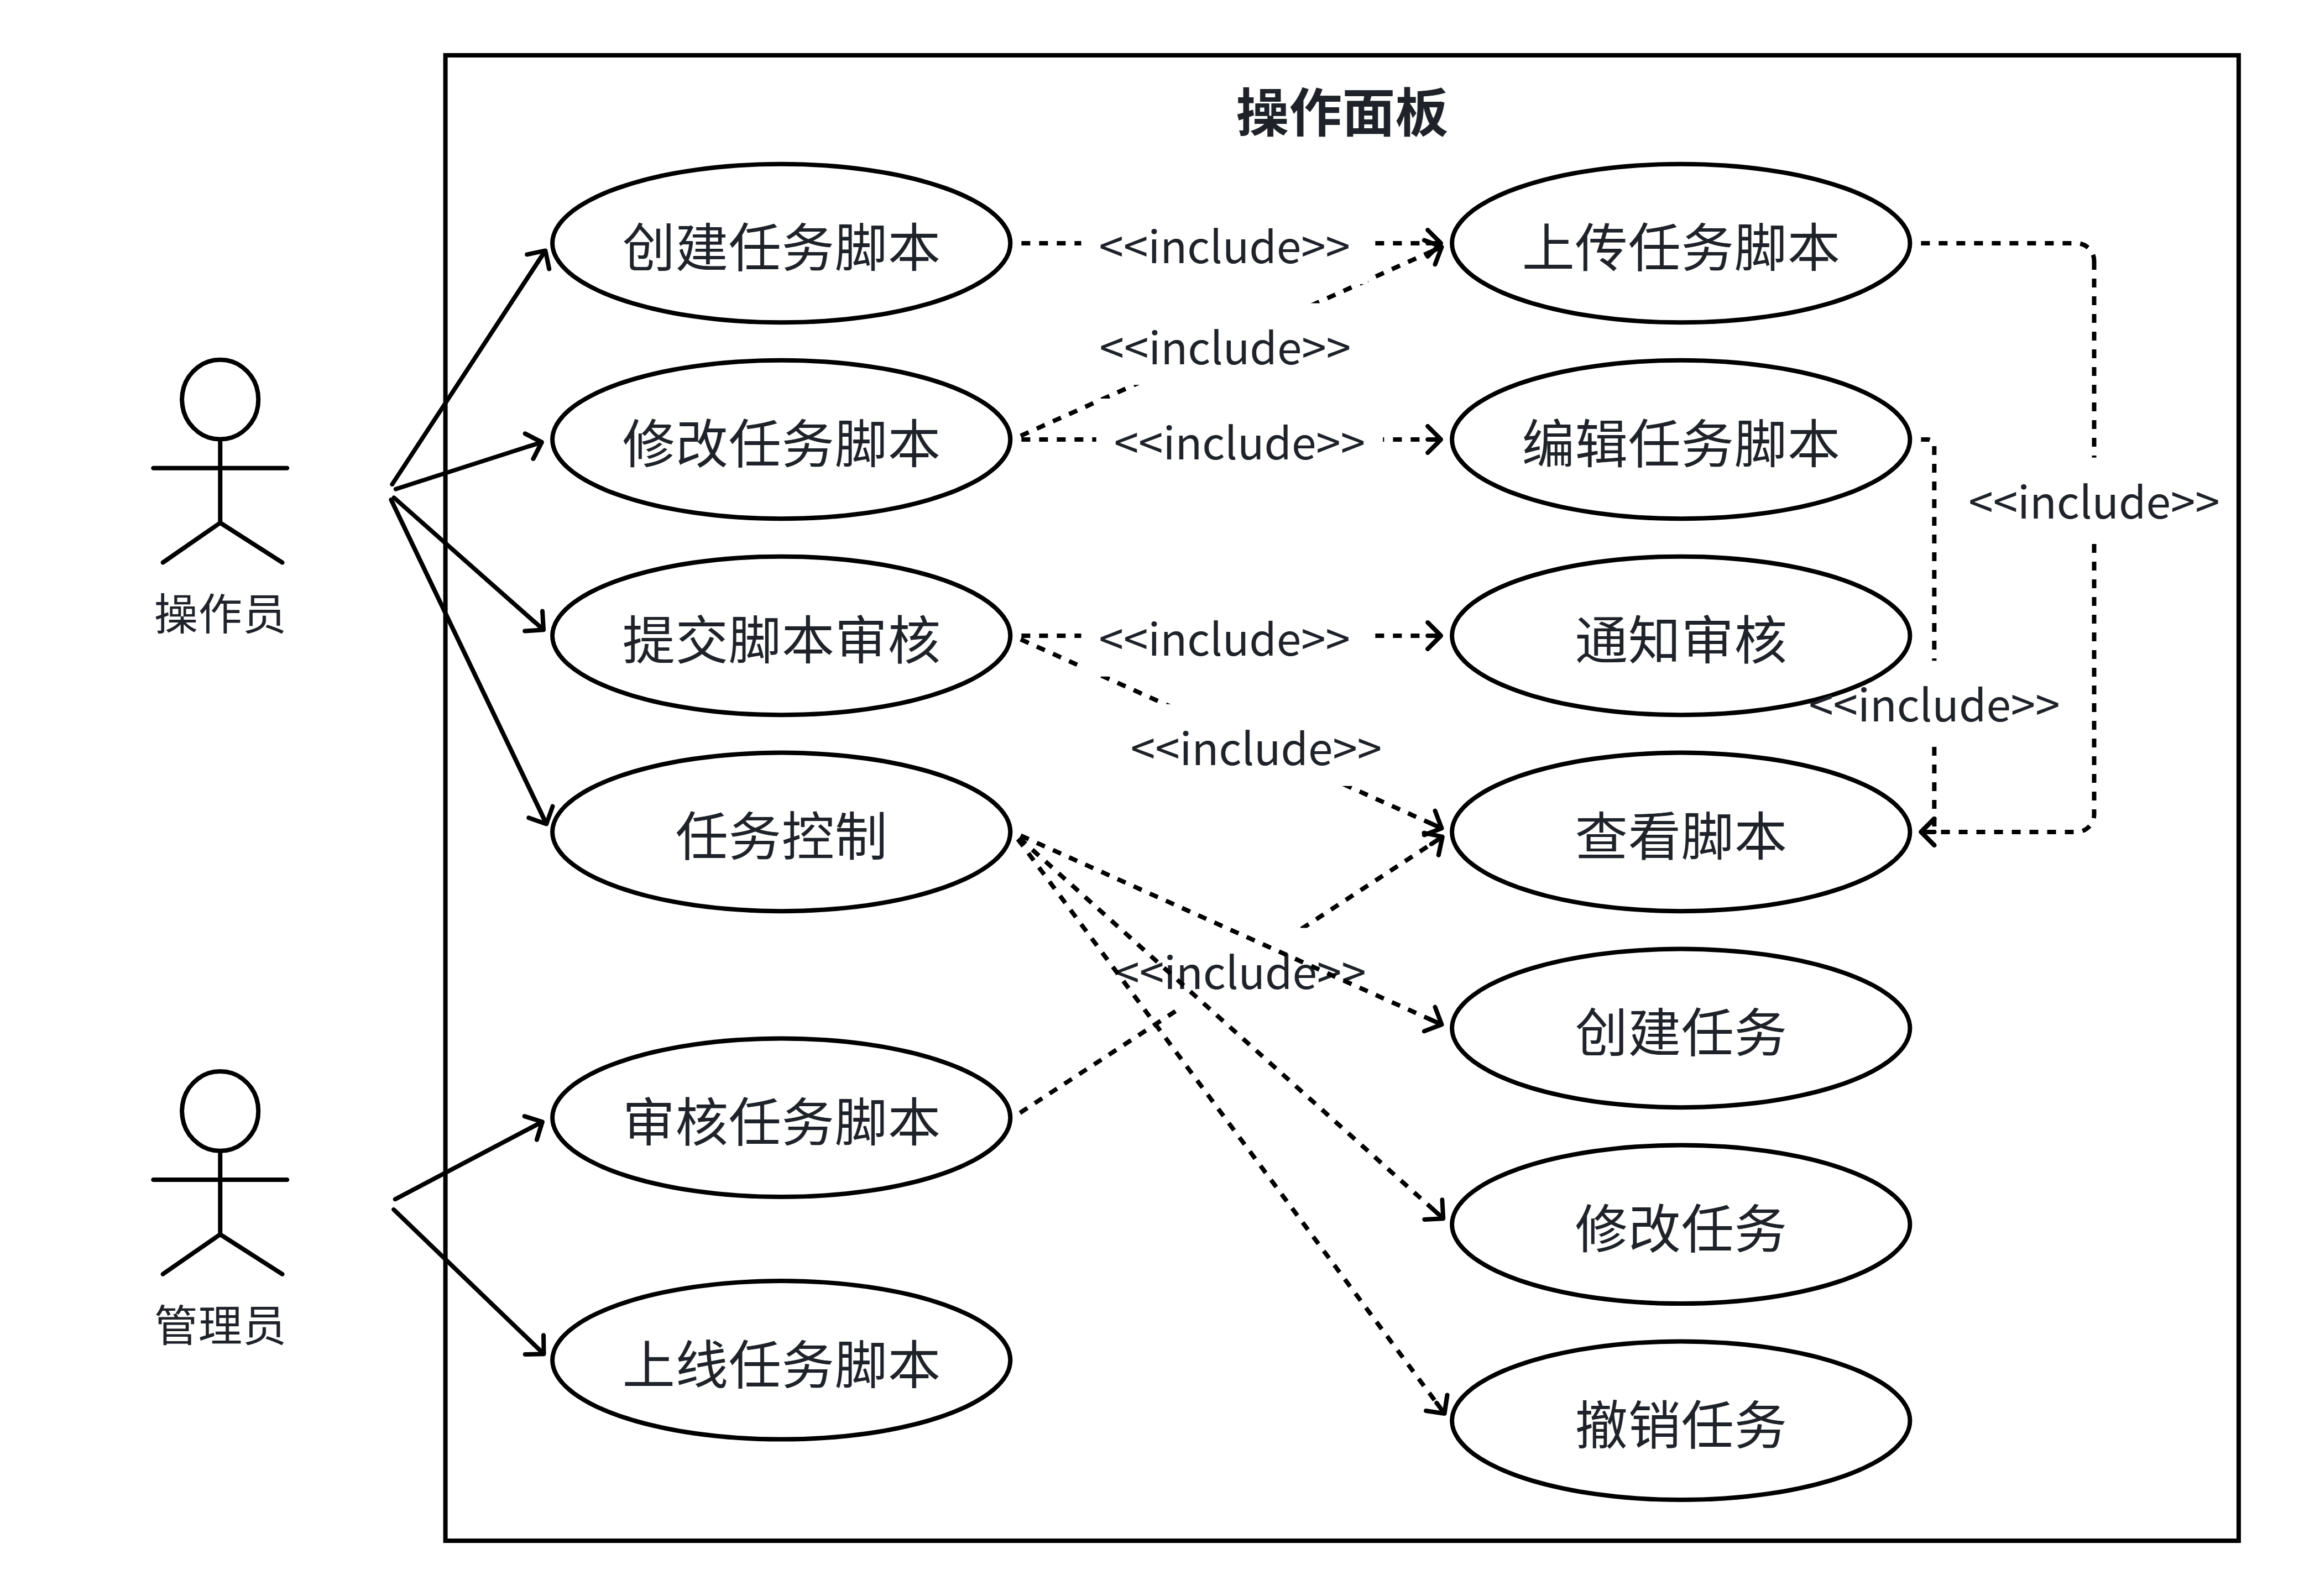
\includegraphics[width=\linewidth]{figures/3/任务操作用例图.png}
    \caption{任务操作用例图}
    \label{fig:enter-label}
\end{figure}

\subsection{权限鉴定}

本系统部署于公司内网环境，为有效防范误操作并规避潜在的数据泄露风险，必须建立严密的身份鉴权与访问控制机制。此外，针对开源生态中的版权归属困境及行业合规管理要求，系统需通过细粒度的权限策略确保安全合规。本系统设计了基于“任务组”的权限模型，将用户划分为系统管理员与操作员两类角色：

\begin{enumerate}
    \item 系统管理员：拥有全局最高权限，负责任务分组的创建、资源配置及对操作员的授权管理。
    \item 操作员：在获得对应任务组授权后，可独立执行任务实例的创建、修改及撤销操作。为强化逻辑安全性，操作员发起的脚本上传或代码修订须经管理员审批通过后方可生效。
\end{enumerate}

这种分层授权的设计模式，既通过管理员的审批把控保障了系统核心逻辑的安全，又赋予了操作员在授权范围内自主处理任务的灵活性，有效平衡了安全管控与运维效率。本系统的权限系统用例图如图3.2所示。

\begin{figure}[htbp]
    \centering
    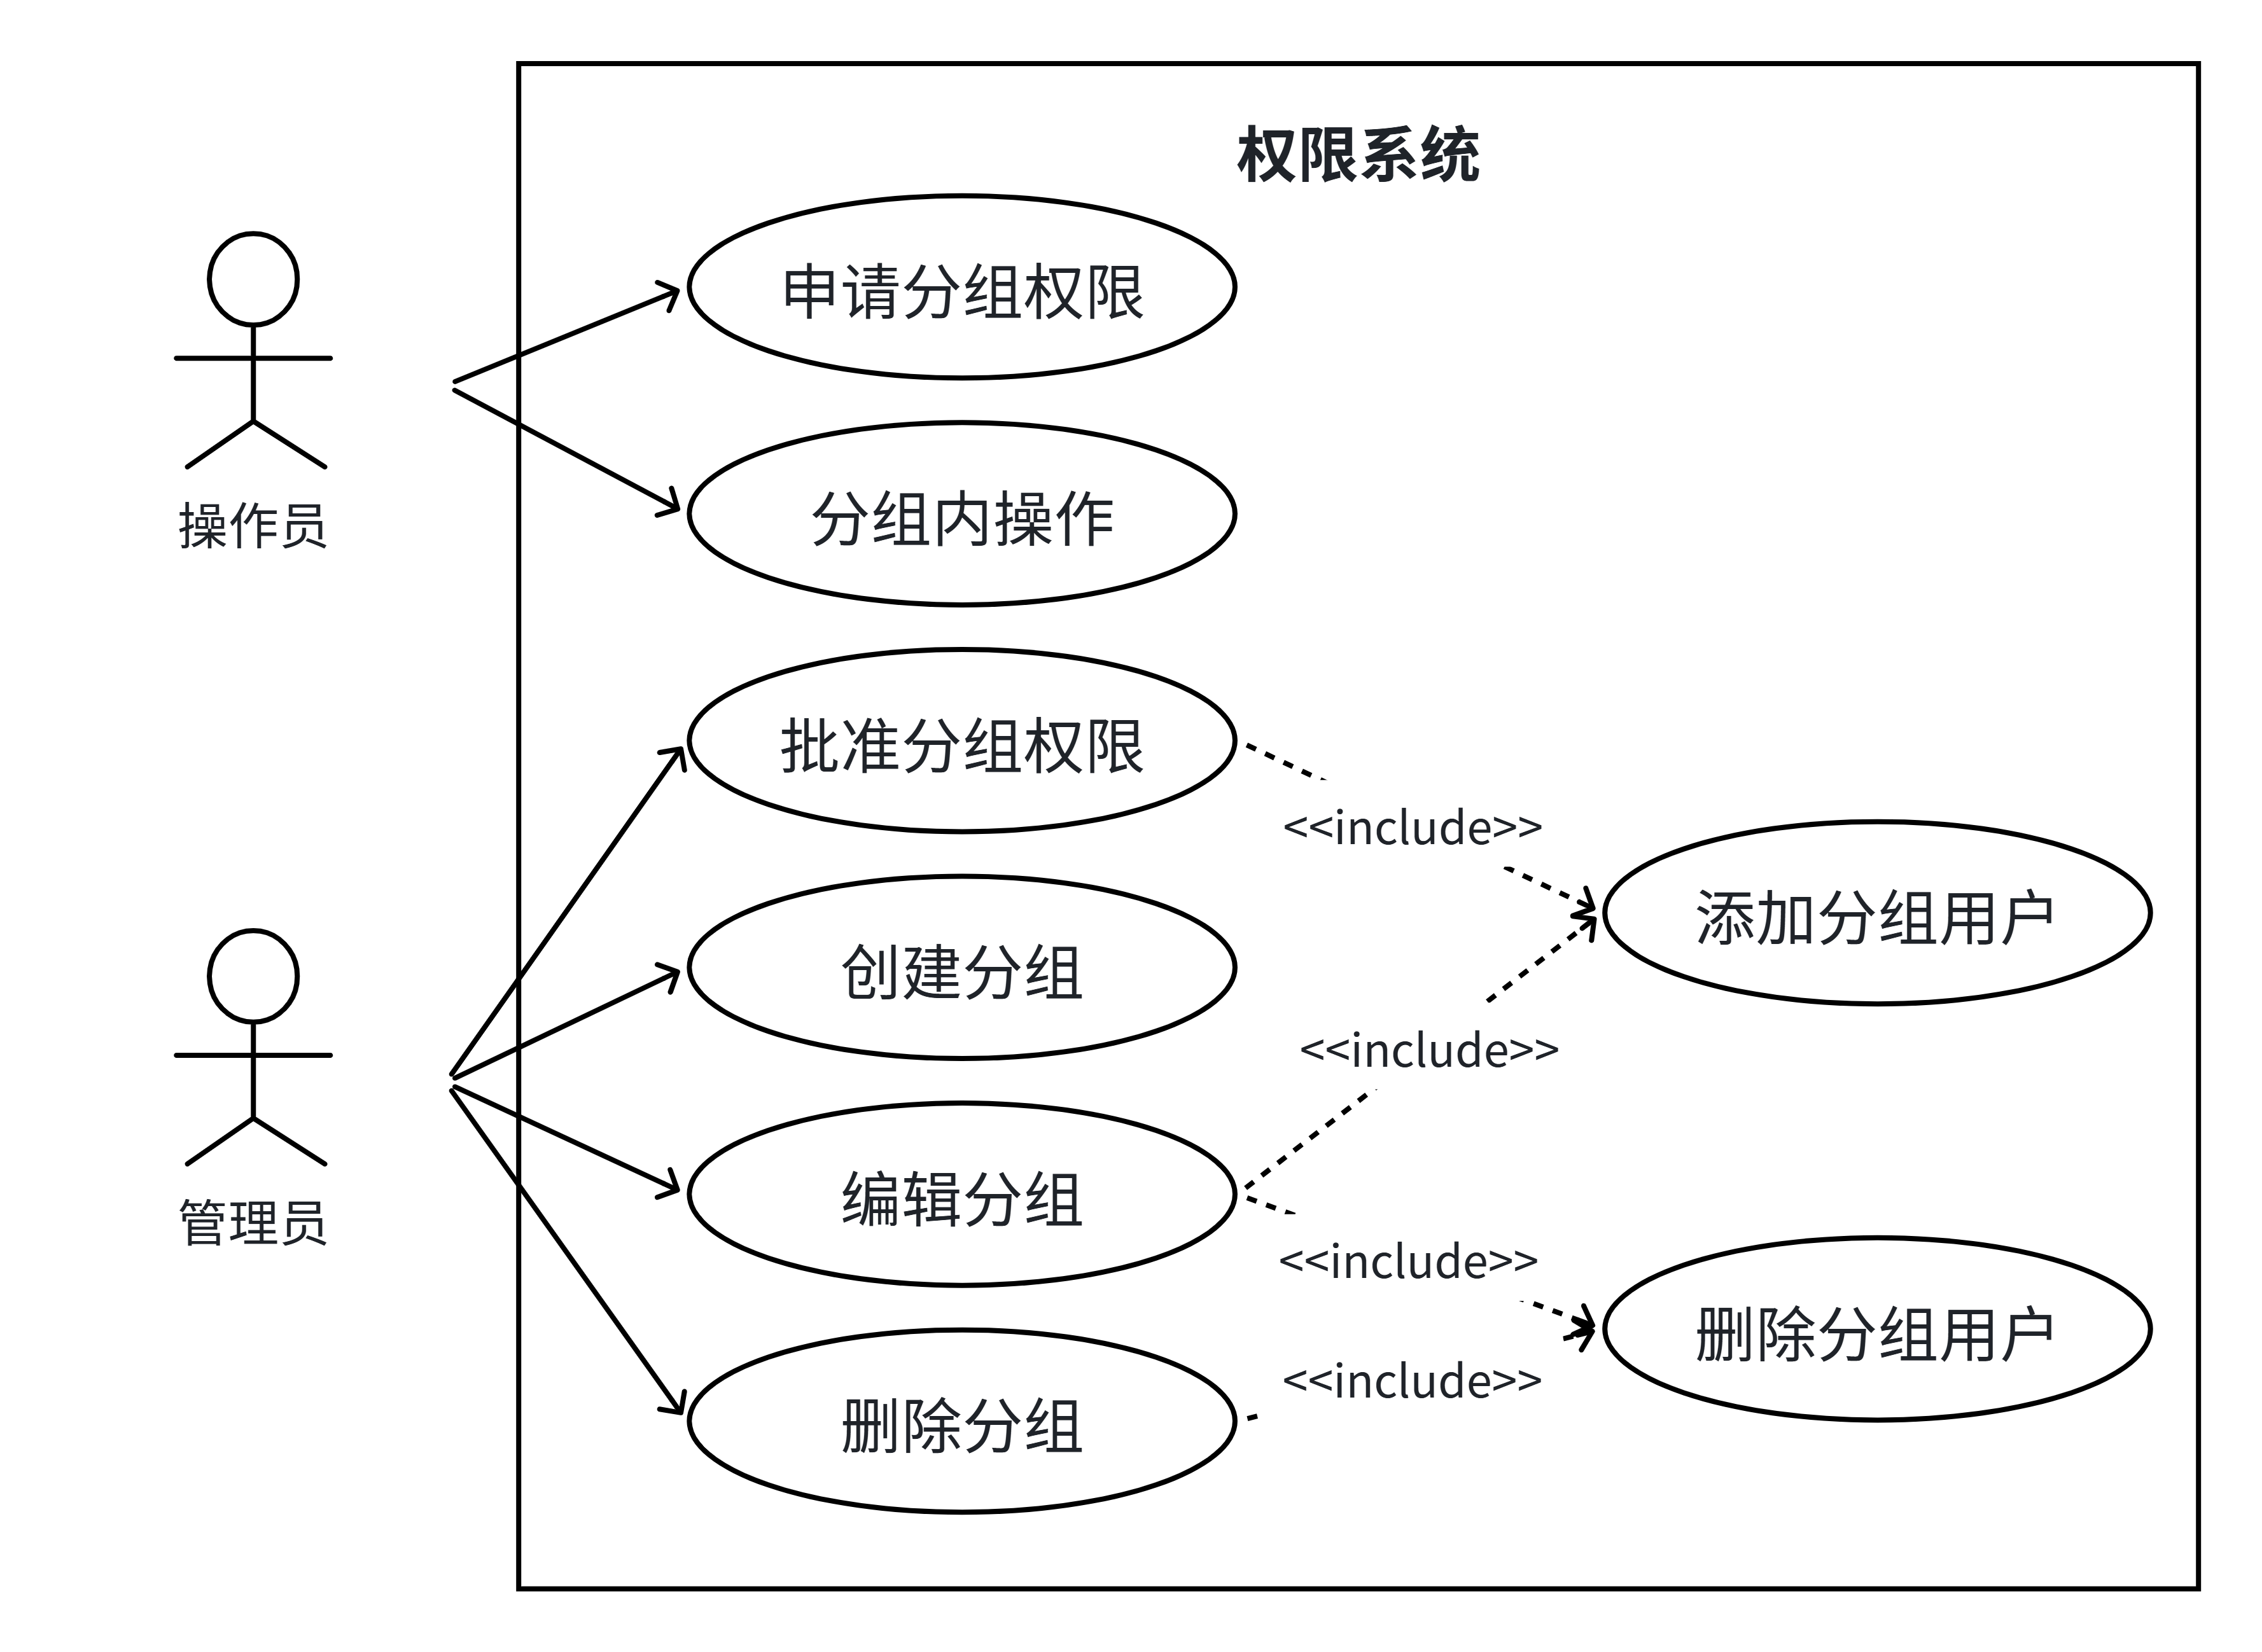
\includegraphics[width=\linewidth]{figures/3/权限系统用例图.png}
    \caption{权限系统用例图}
    \label{fig:enter-label}
\end{figure}

\subsection{数据校验与自动纠正}

为有效解决子问题一中提到的系统对AI特性适配不足及数据处理能力匮乏的问题，API接入层须具备深度的数据感知与鲁棒性纠偏能力。针对AI多任务场景下参数异构、格式复杂的特点，本系统构建了双层校验与修正机制，旨在从源头保障数据的准确性与一致性。

异构数据类型过滤与标准化校验。鉴于Python作为动态类型语言在编译期缺乏强制约束，系统引入了基于Pydantic库的数据验证层。通过建立大模型任务参数画像，对API请求实施实时结构化扫描，强制约束Prompt模板及模型超参数等字段符合预定义的Schema规范，从底层规避因类型不匹配导致的任务崩溃风险。

特定参数自动化纠偏机制。针对操作员录入过程中高发的非致命性逻辑偏差，系统设有智能纠正模块以提升交互容错性。具体包括：自动将全角标点转化为标准半角字符以适配列表处理；识别并剔除复制粘贴产生的冗余括号符号；以及在不损失数值精度的前提下实现浮点数向整数的自动推断与转化。

数据鲁棒性与运维效能优化。该机制通过在接入端预先拦截并修复格式偏差，显著降低了系统的操作门槛与无效请求的重试频率。这不仅保障了下行至调度层与执行层数据的纯净度，也为后续实现复杂的自动化调度闭环奠定了可靠的数据基础。

本需求相关用例如表3.1所示。

\begin{table}[htbp]
\centering
\caption{数据校验与自动纠正功能用例表}
\begin{tabularx}{\textwidth}{lllXl}
\toprule
\textbf{用例ID}&\textbf{用例名称}&\textbf{处理类型}&\textbf{核心操作}&\textbf{处理结果}\\
\midrule
UC-DV-001&AI参数画像匹配&校验&匹配Prompt/超参数Schema&合法通过\\
UC-DV-002&异构类型校验&校验&基于Pydantic实施类型检查&合法通过\\
UC-DV-003&全角标点纠偏&纠正&全角符号向半角标点转化&修正通过\\
UC-DV-004&冗余符号清理&纠正&剔除冗余括号空格等&修正通过\\
UC-DV-005&数值类型推断&纠正&浮点数向整数无损转化&修正通过\\
UC-DV-006&字符串格式化&纠正&去除首尾空格及不可见字符&修正通过\\
UC-DV-007&日期格式统合&纠正&统一日期字符串为“YYYY-MM-DD”&修正通过\\
UC-DV-008&校验结果反馈&反馈&汇总校验报告并下发提示&返回报告\\
\bottomrule
\end{tabularx}
\label{tab:data_validation_cases}
\end{table}

\section{任务调度层功能需求分析}

任务调度层作为本系统的核心逻辑中枢，承担着从任务接入到分发执行之间的关键决策与协调职能。任务调度和资源分配是与服务稳定性、用户满意度以及资源利用率直接相关的两个主要问题\cite{pan2025}。本章将深入剖析该层的功能需求，旨在通过技术手段解决人工智能多任务场景下的自动化决策与算力资源治理难题，具体需求如下：

环境感知的自动化决策：改变传统模式下过度依赖人工判断任务启动时机的现状。系统需具备任务可用性检测功能，通过逻辑引擎实时感知系统负载与运营策略，自主判定任务执行条件，消除调度过程中的人工干预环节。

算力资源的精细化管控：针对GPU等昂贵且稀缺的AI临界资源，系统需建立完备的资源可用性检测机制。通过识别任务间的资源依赖拓扑，精准处理资源互斥冲突，打破传统“保守串行”的限制，在保障数据安全的前提下实现高效的并发调度。

保障分布式环境下的稳健运行：面对异构集群带来的性能差异，系统需支持智能负载均衡，通过权重轮询等算法优化算力分配。同时，构建可靠的数据同步机制与容错恢复体系，确保在网络抖动或算力过载等异常场景下，任务流程依然具备强劲的鲁棒性与自愈能力。

通过上述功能维度的深度分析，本层将建立起一套覆盖智能感知识别、资源动态博弈与高可用性保障的调度体系，为AI研发效能的提升提供坚实支撑。

\subsection{任务可用性检测}

针对子问题二中“调度决策过度依赖人工判断”导致的效能瓶颈，系统需建立具备环境感知能力的自动化决策体系。本系统定义的AI任务在底层实现上表现为支持动态编辑与更新的Python函数，通过调用大模型接口协同输入数据完成特定业务功能。

在传统调度模式下，任务启动时机完全取决于操作员的人工经验，难以精准应对高动态的系统负载环境，系统亟需构建一套基于环境感知策略驱动的逻辑引擎，以解决人工判断的局限性。该引擎需支持管理员通过预设的配置规则（如系统负载阈值、特定场景约束等），将复杂的运营策略转化为可自动执行的决策逻辑。通过这种方式，系统能依据实时负载动态判定任务的执行可行性，实现调度权力由“人工干预”向“引擎自决”的自动化转型，从而在保障业务连续性的同时，显著提升多任务环境下的全局调度效能。本需求的用例表如表3.2所示。

\begin{table}[htbp]
    \centering
    \caption{任务可用性检测功能用例表}
    \begin{tabular}{llll}
        \toprule
        \textbf{用例ID} & \textbf{用例名称} & \textbf{核心操作} & \textbf{处理结果} \\
        \midrule
        UC-TA-001 & 系统负载检测 & 实时采集系统负载值 & 输出负载状态 \\
        UC-TA-002 & 负载阈值配置 & 管理员设置负载阈值 & 保存配置生效 \\
        UC-TA-003 & 任务启动判断 & 对比负载与阈值 & 允许/禁止启动 \\
        UC-TA-004 & 高负载任务限制 & 过载时拦截高耗任务 & 拦截并提示 \\
        UC-TA-005 & 配置修改记录 & 保存管理员配置操作 & 生成操作日志 \\
        UC-TA-006 & 异常场景触发 & 节假日等场景激活规则 & 自动启用限制 \\
        UC-TA-007 & 任务拦截反馈 & 告知用户拦截原因 & 提示负载过高 \\
        UC-TA-008 & 负载回落恢复 & 负载低于阈值时 & 恢复任务启动 \\
        \bottomrule
    \end{tabular}
    \label{tab:task_availability_cases}
\end{table}

\subsection{资源可用性检测}

针对子问题三中“因缺乏资源互斥智能分析能力致使任务盲目串行、算力利用率低下”的痛点，系统需构建精细化的资源感知与管控机制。AI任务在执行过程中对高性能算力资源（如GPU显存、专用硬件等）具有强独占性特征。若两个任务试图同时调用同一临界资源，将引发严重的资源抢占冲突，导致数据错乱或运行失败。

为此，本系统需设计一套基于资源拓扑识别的互斥智能分析机制，以取代传统低效的保守调度策略。首先，系统需建立完备的资源注册体系，强制要求任务在提交时声明其所需的临界资源清单。其次，调度层需具备动态分析能力，通过计算在途任务间的资源依赖拓扑，精准识别各任务间的互斥状态。若判定任务具备执行条件（即目标资源空闲且无互斥冲突），系统应立即触发并发调度；若检测到资源冲突，则需将其加入高可靠等待队列，直至临界资源释放后由调度器自动唤醒。通过这种精细化的资源管控，旨在打破传统模式下的串行执行瓶颈，将调度逻辑由“保守串行”向“安全并发”转变，从而显著压低算力资源的闲置率，提升系统整体吞吐性能。本需求的用例表如表3.3所示。

\begin{table}[htbp]
    \centering
    \caption{资源可用性检测功能用例表}
    \begin{tabular}{llll}
        \toprule
        \textbf{用例ID} & \textbf{用例名称} & \textbf{核心操作} & \textbf{处理结果} \\
        \midrule
        UC-RA-001 & 资源提前注册 & 任务声明所需资源并登记 & 资源信息入库 \\
        UC-RA-002 & 任务资源声明 & 任务提交时标注资源需求 & 记录任务-资源关联 \\
        UC-RA-003 & 任务互斥判定 & 比对任务所需临界资源 & 识别互斥任务 \\
        UC-RA-004 & 执行权限判断 & 检查目标资源占用状态 & 允许/拒绝执行 \\
        UC-RA-005 & 任务等待入队 & 无资源时标记任务状态 & 加入资源等待队列 \\
        UC-RA-006 & 资源释放监测 & 实时跟踪资源占用变化 & 捕获资源空闲状态 \\
        UC-RA-007 & 等待任务唤醒 & 资源空闲时触发队列调度 & 唤醒等待任务执行 \\
        UC-RA-008 & 互斥冲突提示 & 告知用户任务互斥原因 & 提示资源被占用 \\
        \bottomrule
    \end{tabular}
    \label{tab:resource_availability_cases}
\end{table}

\subsection{负载均衡及性能优化}

在本系统分布式架构中，任务执行节点(Worker)表现出显著的硬件与软件异构性。受限于物理基础（如CPU核心、内存容量及I/O吞吐）、运行环境（OS版本、依赖库差异）以及部署策略的不同，各节点间的算力输出与资源偏好天然存在差异。例如，搭载高性能GPU的节点专精于大模型推理，而普通节点则侧重于通用逻辑处理，资源配置重心截然不同。若沿用传统的均等化调度模式，不仅无法有效适配节点间的算力差异，还容易导致高价值资源在峰值期间被无效抢占，进一步加剧了子问题三中提到的算力浪费与任务阻塞难题。

为突破上述瓶颈，系统需构建一套基于实时状态感知与任务需求建模的负载均衡机制。该机制要求调度层精准采集各Worker的实时负载指标（涵盖CPU/内存利用率、队列长度及剩余算力评估），并动态分析各类AI任务的资源亲和性特征。通过引入智能权重分配算法，系统应实现任务与节点的最佳匹配：将计算密集型训练或推理任务优先指派至算力充裕的GPU节点，而将参数处理等轻量级任务分发至响应及时的通用节点。这种精细化的调度方案不仅能有效规避单点过载引发的任务堆积，更能充分释放异构集群的算力潜力，确保在应对多任务高并发场景时，系统始终保持高吞吐与低延迟的稳健运行状态。

\subsection{数据同步}

在分布式AI调度体系中，任务流转涉及复杂的Prompt模板、模型超参数及大规模异构中间数据。子问题一明确指出，现有系统对AI特性的适配性不足，主要体现在异构参数处理与数据类型分析能力的缺失上。若各子模块（如任务创建、执行、存储模块）间的数据同步机制存在缺陷，API接入层预先完成的参数纠偏与类型推断结果将无法准确、完整地透传至任务执行节点。这种数据流转过程中的失真与偏差，不仅会导致任务执行逻辑偏离预设轨道，产生与实际需求相悖的无效结果，更会因频繁的数据回溯与重复执行而造成高昂算力资源的严重浪费。

为攻克适配性难题，系统亟需构建一套高可靠、强一致的数据同步机制，作为保障AI任务顺畅推进的核心支撑。该机制需深度对接大模型任务参数画像，确保异构数据映射结果与自动纠偏策略在任务生命周期的各阶段保持实时一致。当任务在不同子模块间流转时，系统必须保障Prompt配置、中间计算结果及执行状态标识的高度同步，消除因子模块数据差异导致的决策瓶颈。通过建立基于高性能中间件的消息同步底座，系统旨在实现数据的透明流转与闭环管理，为任务的稳定运行及后续的算力精准调度提供坚实的数据基础。

\subsection{容错与恢复}

针对系统适配性欠佳及异构数据处理能力不足的问题，系统需构建完善的容错与自动化恢复机制，以保障AI任务在复杂生产环境下的性能表现与持续稳定性。AI任务普遍具有高算力消耗与执行周期长的特征，任何非预期的流程中断都会造成昂贵计算资源的无效浪费。因此，系统应具备对非致命性异常的动态识别与自助修复能力，通过重试逻辑或参数自动纠偏手段完成初步恢复。在确保任务连续性的同时，系统需实现异常处理的静默化，从而最大限度降低操作员的运维频率与心智负担。结合生产环境的实际需求，系统需重点针对以下两类异常场景建立自愈策略：

\begin{enumerate}
    \item 网络通信韧性保障：尽管系统部署于公司内网，但由于内网拥堵引发的超时风险依然存在。系统需将超时视为典型的可恢复异常，并依据预设规律（如指数退避机制）进行自动重试。这不仅能保障调度响应的及时性，还能有效增强系统在复杂网络环境下的运行韧性。
    \item 数据类型自愈与纠偏：受分布式架构中子模块版本更新不及时等因素影响，系统常遭遇异构数据传输导致的参数错误，如浮点数（float）与整数（int）类型冲突。基于子问题一的适配性要求，系统需内置智能纠偏规则，对简单的类型不匹配、字符输入偏差（如全角/半角标点混用）或逻辑拼写失误进行实时修复与无损转化，确保下行指令的准确性与鲁棒性。
\end{enumerate}

通过建立多级容错恢复体系，系统旨在实现从“人工排查异常”向“系统自动感知与治理”的深度转型，从根本上解决调度流程中的性能瓶颈与稳定性隐患。

\section{任务执行层功能需求分析}

本系统采用分布式微服务架构，任务执行层作为算力调度的最终落地单元，需直接面对AI大模型任务高算力、长周期及数据异构等核心特征。针对现有调度体系在AI特性适配性上的局限，以及对异构数据处理与类型分析能力的不足，本层通过构建标准化的参数传递协议、灵活的任务编辑机制以及深度的异常捕获流程，确保API接入层完成的参数纠偏与数据画像结果能够精准转化为算力输出。在这种独特的部署模式下，如何保障复杂AI参数在跨节点传输时的准确性，以及在执行过程中对资源占用的即时响应，衍生出了以下关键功能需求。接下来，本章将深入剖析这些功能需求的具体内容及其设计的必要性。

\subsection{参数传递}

基于系统灵活性与可扩展性的工程考量，本系统采用分布式微服务架构，将“任务调度层”与“任务执行层”解耦部署于不同的计算节点。在这种物理隔离的架构下，AI任务指令与超参数无法通过传统的本地函数调用进行交互，必须依赖复杂的网络环境完成跨节点传输。针对现有调度体系在AI异构数据处理及环境适配能力上的缺失，执行层在接收参数后需建立一套深度适配机制，无法直接投入计算。由于深度学习算法具有极强的数据依赖性，系统必须在任务启动前执行参数预处理逻辑。例如，需自动化完成大规模远程附件的并发拉取，并动态执行参数画像中的路径重定向，将远程URL映射为本地物理路径，以确保任务脚本在异构执行环境下的逻辑一致性。为确保AI异构参数在分布式环境下的高效流转，本系统在参数传递环节需满足以下核心需求：

\begin{enumerate}
	\item 透明传输：对于操作员以及本系统的各个子模块而言，在参数的发送与接收过程中，应实现无感操作，就如同进行本地系统调用一般。为此，本层需具备支持任意类型和大小参数的能力。
	\item 可靠传输：本系统需确保参数传递的准确性。因为传递错误的参数极有可能致使任务出现异常，进而导致结果无效。此外，系统还应保障任务与参数能够可靠传达，即能够及时察觉任务丢失问题，并采取重试措施。
	\item 远程附件拉取：部分任务依赖远程附件，对此，本系统需预先准备好这些附件，并将对应的参数修改为本地路径，以便任务能够无感知地读取附件。
\end{enumerate}

本系统参数传递功能用例表如表3.4所示。

\begin{table}[htbp]
    \centering
    \caption{参数传递功能用例表}
    \begin{tabular}{llll}
        \toprule
        \textbf{用例ID} & \textbf{用例名称} & \textbf{核心操作} & \textbf{处理结果} \\
        \midrule
        UC-PT-001 & 参数封装处理 & 打包任意类型参数 & 生成传输数据包 \\
        UC-PT-002 & 透明传输处理 & 屏蔽网络传输细节 & 实现无感调用 \\
        UC-PT-003 & 传输校验机制 & 验证参数完整性 & 确保数据准确 \\
        UC-PT-004 & 任务丢失检测 & 监控传输状态 & 发现丢失触发重试 \\
        UC-PT-005 & 远程附件拉取 & 下载远程附件至本地 & 生成本地文件路径 \\
        UC-PT-006 & 参数路径替换 & 将远程路径改为本地路径 & 适配本地执行环境 \\
        UC-PT-007 & 断点续传支持 & 大参数分片传输 & 支持中断后继续 \\
        UC-PT-008 & 传输结果反馈 & 返回参数处理状态 & 告知成功/失败原因 \\
        \bottomrule
    \end{tabular}
    \label{tab:parameter_transfer_cases}
\end{table}

\subsection{任务编辑}

在AI大模型任务的实际执行过程中，面对参数空间呈指数级增长的调优需求，以及业务指标随环境波动而产生的高度不确定性，受限于模型超参数的复杂性以及业务需求的动态演进，操作员常需对已提交或正在运行的任务进行参数微调或类型修正。然而，传统的调度模式往往缺乏对执行中任务的即时干预能力，使得系统极易陷入“预设指令”与“实际需求”脱节的僵化状态。

若无法实现任务的动态编辑，将导致由于操作疏忽引发的错误逻辑持续空耗昂贵的计算资源，甚至造成核心算力集群的长效阻塞。因此，任务执行层必须构建一套高可靠的撤销与重启机制。这不仅是为了赋予操作员灵活的容错纠偏能力以回应数据适配挑战，更是为了确保在变更发生时，能够通过对底层进程的精细化治理，即时终止异常进程并释放被独占的GPU等临界资源，从而最大化算力周转效率，避免无效负载对硬件寿命与研发周期的双重损耗。同时，重启后的新任务必须重新联动自动化决策引擎，结合当前集群的负载实况与策略权重，重新判别其是否满足最新的执行条件。
具体的撤销与重启机制需满足以下几点要求：

\begin{enumerate}
	\item 及时终止对应进程：在AI系统中，算力资源极为宝贵。因此，及时终止旧进程以节约算力，显得尤为重要。
	\item 及时释放对应资源：本系统存在诸多仅能互斥使用的资源。及时释放这类资源，有助于提高本系统的并发处理能力，缩短其他任务的执行周期，进而提升系统吞吐量。
	\item 判断新任务是否满足运行要求：旧任务撤销后，新任务启动需满足本系统的两个条件：其一，依据运营策略计算得出任务可执行；其二，任务所依赖的资源未被占用。本系统需在发送新任务前，重新进行上述计算。
\end{enumerate}

本系统任务编辑功能用例表如表3.5所示。

\begin{table}[htbp]
    \centering
    \caption{任务编辑功能用例表}
    \begin{tabular}{llll}
        \toprule
        \textbf{用例ID} & \textbf{用例名称} & \textbf{核心操作} & \textbf{处理结果} \\
        \midrule
        UC-TE-001 & 任务撤销触发 & 接收操作员撤销指令 & 启动终止流程 \\
        UC-TE-002 & 任务参数修改 & 编辑任务参数及类型 & 保存修改内容 \\
        UC-TE-003 & 任务重启执行 & 符合条件时启动新任务 & 任务进入运行态 \\
        UC-TE-004 & 操作结果反馈 & 返回撤销/重启状态 & 告知成功/失败原因 \\
        \bottomrule
    \end{tabular}
    \label{tab:task_editing_cases}
\end{table}

\subsection{异常捕获}

本系统在任务执行过程中，可能会遭遇多种异常情况，诸如k8s的CPU Limit（即CPU受限）问题、内存受限问题等。以系统迭代过程中的一个真实案例为例，操作员上传了一段存在问题的Python代码。此代码包含发送数据包的业务逻辑，但在完成数据包发送后，却未及时关闭相应的文件描述符（file descriptor）。结果在数小时内，系统内存占用量持续攀升，最终引发异常，导致操作员前期投入的工作成果失效。该案例将在后续“系统测试与分析”章节中详细阐述，在此提及旨在表明，本系统有必要设计一套异常捕获机制。借助这一机制，能够及时监控并分析系统出现的异常状况，及时上报异常信息并尝试恢复系统正常运行，这将极大地节省操作员的工作量，有效提高工作效率。本系统的异常捕获与恢复机制，需要满足如下几点要求：
\begin{enumerate}
	\item 全面且细致地监测系统各项指标，针对诸如CPU、内存、文件描述符等易对系统稳定性产生影响的关键指标，构建基于历史数据的预测机制。一旦发现问题，即刻通知相关人员。如有必要，及时暂停相关任务，并暂存相关数据，以此避免数据丢失及工作量的浪费。
	\item 异常信息采集：依托Python的异常处理流程，本系统能够构建一套完备的异常信息采集机制。当任务出现异常时，系统应及时采集异常信息，并通知相关人员。详尽的异常信息有助于相关人员分析错误原因，进而修复错误，及时止损并促使系统恢复正常运行。
\end{enumerate}

这不仅将极大地减轻操作员的人工值守负担，将从繁琐的故障排查中解放出来，更能有效保障昂贵计算资源的周转效率，从而在整体工程维度上实现开发与运维效率的跨越式提升。

本系统异常捕获功能用例表如表3.6所示。

\begin{table}[htbp]
    \centering
    \caption{异常捕获功能用例表}
    \begin{tabular}{llll}
        \toprule
        \textbf{用例ID} & \textbf{用例名称} & \textbf{核心操作} & \textbf{处理结果} \\
        \midrule
        UC-EC-001 & 系统指标监测 & 实时采集CPU/内存/文件描述符 & 输出指标数据 \\
        UC-EC-002 & 异常预测预警 & 识别指标异常 & 触发预警通知 \\
        UC-EC-003 & 异常任务暂停 & 终止目标任务 & 避免资源浪费 \\
        UC-EC-004 & 任务数据暂存 & 暂停任务前保存中间数据 & 防止数据丢失 \\
        UC-EC-005 & 异常捕获 & 异常流程采集信息 & 获取异常日志 \\
        UC-EC-006 & 异常信息上报 & 推送详情至相关人员 & 通知处理故障 \\
        UC-EC-007 & 异常原因分析 & 整理数据辅助排查 & 提供分析依据 \\
        UC-EC-008 & 系统恢复尝试 & 重启服务释放资源 & 恢复系统运行 \\
        \bottomrule
    \end{tabular}
    \label{tab:exception_capture_cases}
\end{table}

\section{非功能需求}

非功能需求作为系统构建的重要基石，不仅决定了资源调度系统在工业生产环境中的可用边界，更是支撑本文核心研究目标——解决AI多任务场景下适配、决策与资源利用三大瓶颈的关键所在。

具体而言，高性能特性是实现算力资源高效并发调度与动态周转的技术先决条件，直接决定了系统在应对大规模 AI 任务时资源利用率的上限；工业级稳健性则是驱动调度决策机制由传统人工干预向全自动化、自愈式演进的核心保障，确保系统在面临硬件失效或网络波动等极端工况时，仍能维持业务逻辑的持续性与系统状态的一致性；而广泛的兼容性则确保了参数传递机制在分布式异构底座上的逻辑一致性，为系统的规模化工业推广及研发效能的提升提供了底层支撑。

\subsection{性能需求}

系统应具备高并发环境下的实时请求处理能力，核心在于解决子问题三中算力资源利用率低下的痛点。通过将资源互斥智能分析与调度决策的响应延迟控制在极低阈值内，实现对AI算力资源的高效并发周转，旨在消除传统串行模式引发的调度瓶颈。同时，系统在执行批量控制指令与大规模附件流转时需保持高度流畅，以适配AI高频研发场景，确保无明显感知卡顿。根据量化性能指标要求，在10并发的常规工况下，任务提交、删除及编辑的平均响应时间应低于50ms；在100并发的中等压力下，响应时间应控制在100ms以内；即便在1000并发的极端高负载场景下，平均响应时间也需限制在500ms以内且确保系统稳定运行无崩溃。这一性能表现将从技术底层保障子问题二中自动化决策引擎的执行效率，支撑大规模AI任务的快速流转。相关参数需求指标如表3.7所示。

\begin{table}[htbp]
\centering
\caption{性能需求指标表}
\begin{tabular}{lll}
\toprule
测试内容 & 预期结果 \\
\midrule
10 并发下提交任务平均响应时间 & 响应时间 < 50 ms \\
10 并发下删除任务平均响应时间 & 响应时间 < 50 ms \\
10 并发下编辑任务平均响应时间 & 响应时间 < 50 ms \\
100 并发下提交任务平均响应时间 & 响应时间 < 100 ms \\
100 并发下删除任务平均响应时间 & 响应时间 < 100 ms \\
100 并发下编辑任务平均响应时间 & 响应时间 < 100 ms \\
1000 并发下提交任务平均响应时间 & 响应时间 < 500 ms \\
1000 并发下删除任务平均响应时间 & 响应时间 < 500 ms \\
1000 并发下编辑任务平均响应时间 & 响应时间 < 500 ms \\
\bottomrule
\end{tabular}
\label{tab:perf_concurrent}
\end{table}

\subsection{稳定性需求}

系统需保障工业级的长期运行可靠性，具备对各类复杂工况及非致命异常的自动化修复能力。针对子问题二中决策过度依赖人工的局限，环境感知的异常自愈机制应在感知故障后瞬时触发，最大限度缩短业务中断时长，实现调度决策的去人工化与业务连续性保障。为确保在生产环境下的工业级可靠性，所有稳定性测试用例的通过率必须达到100\%，以从底层构筑起覆盖AI任务全生命周期的稳健运行防线。稳定性需求用例如表3.8所示。

\begin{table}[htbp]
\centering
\caption{稳定性需求用例表}
\begin{tabular}{lll}
\toprule
测试内容 & 预期结果\\
\midrule
关机重启 & 程序自动恢复，数据无丢失 \\
断电 & 继续未完成任务 \\
网络中断 & 程序重连网络，任务继续 \\
多任务并发执行 & 任务无冲突，结果正确 \\
磁盘空间不足时 & 提示空间不足，程序停止 \\
\bottomrule
\end{tabular}
\label{tab:my_label}
\end{table}

\subsection{兼容性需求}

在任务执行层的兼容性保障方面，系统必须能够横跨多种主流指令集架构与操作系统组合。具体测试用例涵盖了Linux系统下的x86与ARM服务器，以及Windows系统下的x86与ARM服务器。要求程序能够精准适配底层架构，在各异构算力底座上均能保持稳定运行且无任何报错。为了验证系统对不同计算环境的广泛支持，并确保参数传递机制在分布式节点间的一致性，上述所有兼容性测试用例的通过率必须达到100\%，从而为系统的工业级推广提供坚实的兼容性保障。兼容性需求用例如表3.9所示。

\begin {table}[htbp]
\centering
\caption {兼容性需求用例表}
\begin {tabular}{lll}
\toprule
测试内容 & 预期结果\\
\midrule
Linux系统x86服务器 & 程序适配架构，运行稳定无报错 \\
Linux系统ARM服务器 & 程序适配架构，运行稳定无报错 \\
Windows系统x86服务器 & 程序适配架构，运行稳定无报错 \\
Windows系统ARM服务器 & 程序适配架构，运行稳定无报错 \\
\bottomrule
\end {tabular}
\label {tab:my_label}
\end {table}

\section{本章小结}

本章立足于AI多任务场景下的实际痛点，深度剖析了当前调度体系在AI特性适配、环境决策自律及临界资源管控三大核心维度上的技术局限。通过对业务需求的系统化拆解，本章明确了构建标准化分组管理、异构参数智能纠偏、环境感知调度决策及算力资源互斥识别等功能模块的必要性。这些需求分析不仅为后续章节的架构设计提供了逻辑支撑，更确立了系统由“人工经验驱动”向“智能自动化调度”转型的核心目标，旨在全方位提升AI多任务管理在高并发、异构环境下的稳健性与算力利用率。

\makeatletter
\@openrightfalse
\makeatother
\chapter{概要设计}

本章主要介绍本系统的概要设计，重点针对AI多任务场景下系统适配性差、调度决策太依赖人工以及资源互斥识别难这三大核心子问题，给出了层级化的架构设计思路。整个系统分为API接入层、任务调度层和任务执行层：API层和执行层主要负责解决“适配”问题，通过建立大模型任务参数画像，实现了对AI异构数据的自动纠错与类型推断；任务调度层则是系统的“指挥中枢”，通过引入环境感知的自动化决策引擎和资源互斥智能分析算法，让任务能脱离人工干预自动下发，并有效解决了资源抢占导致的串行效率低下难题。通过这三层架构的紧密协作，系统完成了由传统排队模式向智能化、高并发调度的转型，为后续的功能实现与工业推广打下了坚实的架构基础。

\section{AI多任务资源调度系统基本原则}

为确保系统能够有效应对AI大模型任务的高算力需求与复杂数据特征，本系统在架构设计阶段遵循以下核心原则：

\begin{enumerate}
	\item 异构参数适配与数据鲁棒性原则。针对AI大模型任务参数格式多样且极易出错的特征，系统需在数据接入端强化Schema层级的深度校验。设计应具备对全角/半角符号、非法字符及数据类型的自动纠偏逻辑，确保异构参数在分布式传递过程中的语义一致性，从源头提升系统的容错能力与数据处理门槛。
    \item 环境感知与决策自主化原则。针对任务调度过度依赖人工干预的现状，系统应具备对计算集群负载、网络状态及运营策略的实时感知能力。通过构建基于逻辑引擎的自主决策机制，将传统的“人工触发”转化为“策略驱动”，实现调度流程的自动化闭环，以提升系统在高动态环境下的响应效能。
    \item 临界资源隔离与并发安全原则。算力资源的精准治理是系统的核心目标。设计必须建立细粒度的“资源-任务”映射关系，通过互斥检测算法识别任务间的算力冲突（如GPU显存抢占）。系统应支持在保障资源独占安全的前提下，通过智能并发策略取代传统串行模式，最大化集群吞吐率并降低算力空耗。
    \item 架构分层解耦与弹性扩展原则。系统应遵循模块化设计思想，将API接入、任务调度与分布式执行进行逻辑解耦。各层级间通过标准化协议通信，确保系统具备良好的水平扩展能力，以便在计算负载激增时，能够通过动态增加执行节点（Worker）完成算力的线性扩容。
    \item 细粒度权限管控与合规性原则。鉴于AI算力资源的昂贵性与数据的敏感性，系统必须构建严密的鉴权体系。基于“任务组”实现多租户隔离与访问控制策略（RBAC），严格限制非授权用户对临界资源的占用与调度指令的干预，确保生产环境下的资源分配安全性与审计合规性。
\end{enumerate}
 
\section{AI多任务资源调度系统整体结构}

\begin{figure}[ht]
    \centering
    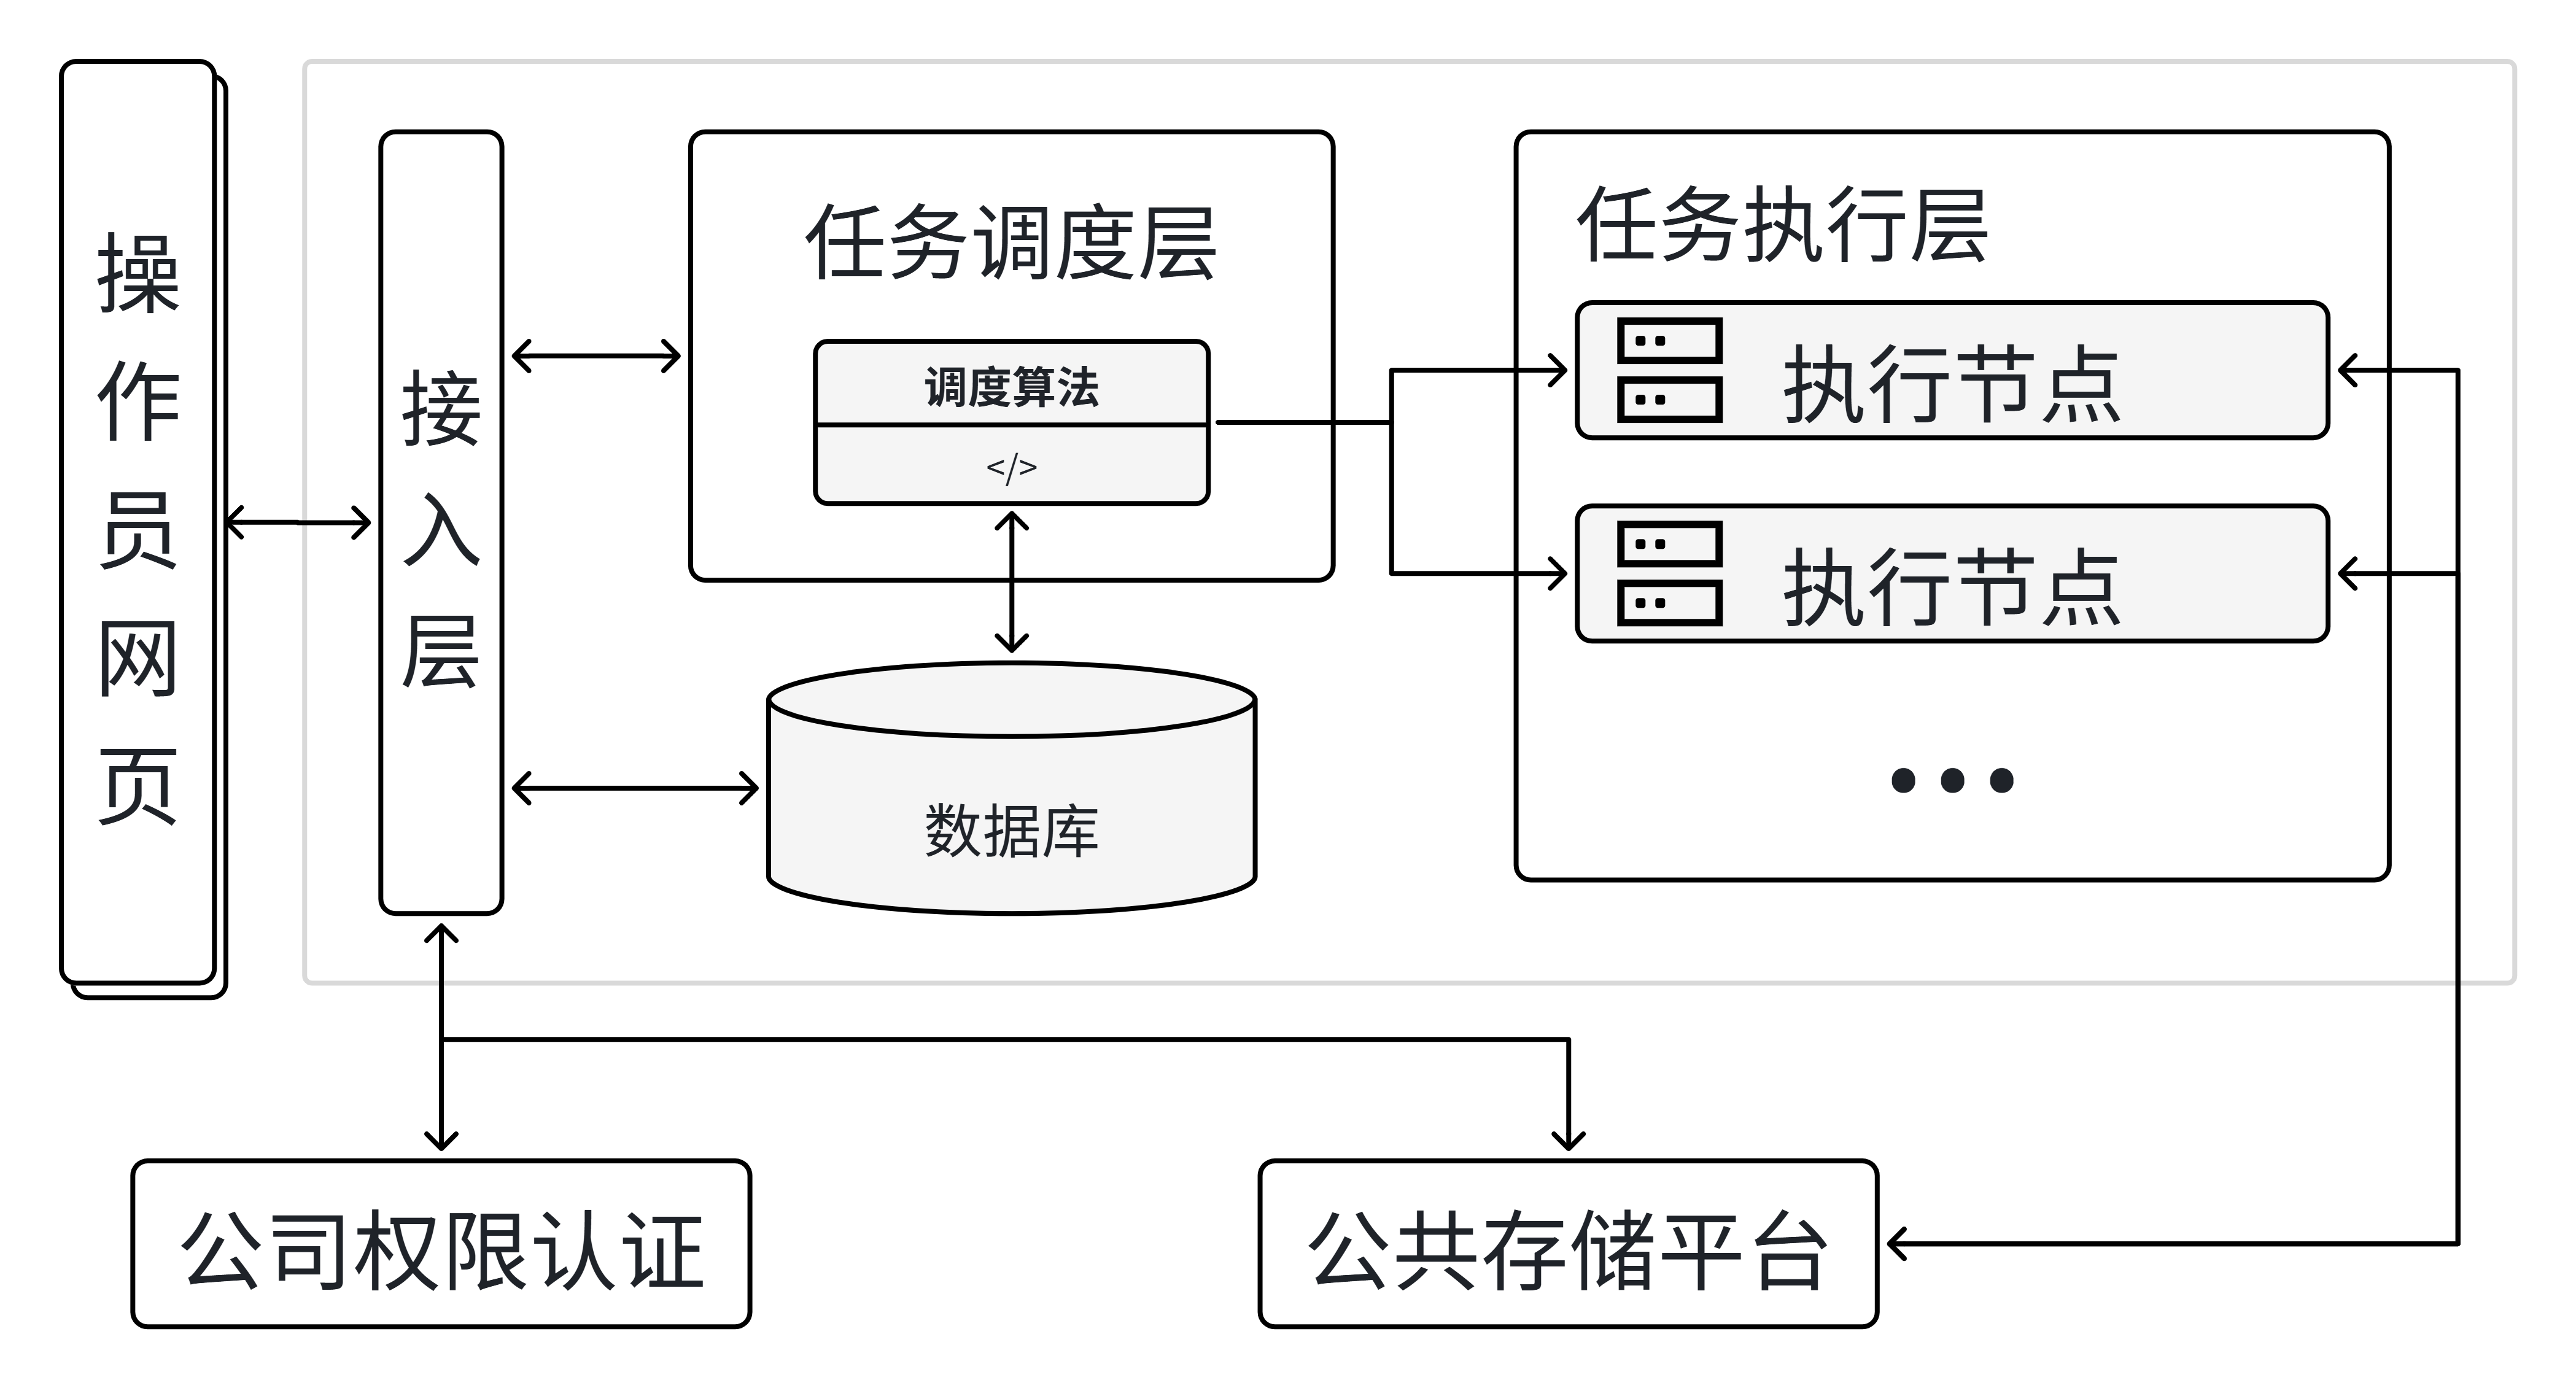
\includegraphics[width=\linewidth]{figures/4/系统整体架构.png}
    \caption{系统整体架构图}
    \label{fig:enter-label}
\end{figure}

本系统整体结构如图4.1所示。为有效应对前文提出的三大核心挑战，系统采用分层解耦的软件架构设计，将复杂的调度逻辑划分为三个功能层级，各层间通过标准化接口进行数据交互，确保系统具备高内效能与良好的扩展性。简要介绍如下：

\begin{enumerate}
    \item API接入层。该层作为系统与外部交互的唯一门户，主要负责请求拦截、身份核验与初步数据治理。针对子问题一，本层重点设计了异构数据自动纠偏机制。在HTTP过滤层完成公司级鉴权后，系统会对输入的Prompt模板及AI超参数进行Schema校验，自动修正字符格式偏差与类型冲突，从源头保障任务数据的纯净度，解决现有系统适配性欠佳的问题。
    \item 任务调度层。该层是系统的决策大脑，由任务池、自动化决策引擎、同步模块及容错恢复模块组成。针对子问题二，调度层通过逻辑引擎实时感知系统负载，自主判定任务执行条件，消除了对人工触发的依赖；针对子问题三，该层引入了临界资源互斥分析算法，通过动态扫描资源占用表，精准识别任务间的算力冲突，将传统的保守串行调度优化为智能并发调度，显著提升了算力利用率。
    \item 任务执行层。该层由分布式的任务执行器（Worker）构成，直接对接公司存储服务与GPU算力资源平台。其内部设有参数本地化处理、任务执行监控及结果上报模块。该层负责接收调度层下发的指令，执行具体的AI模型推理或测试任务。通过细粒度的异常捕获机制，该层能实时反馈节点运行状态，配合调度层的容灾逻辑，确保在异构环境下任务执行的鲁棒性与一致性。
\end{enumerate}

\section{API接入层概要设计}

API接入层承担系统的安全准入与数据治理职能。在承载高并发请求的基础上，该层通过身份鉴权与参数标准化预处理构建合规屏障。本层重点引入参数画像校验与自动纠偏逻辑，在入口处即时拦截并修复人工录入偏差，确保调度指令的高度一致性与鲁棒性，从源头解决AI异构数据的适配难题。

\subsection{权限鉴定模块}

鉴权模块分为两部分：身份认证、权限判定。身份认证功能以一个Python函数的形式注册成为了FastAPI框架的一个中间件。中间件是一种位于操作系统和应用程序之间的软件层，用于解决不同系统之间的数据格式转换、通信协议适配等问题\cite{9}。身份认证功能的时序如下图4.2所示：

\begin{figure}[htbp]
    \centering
    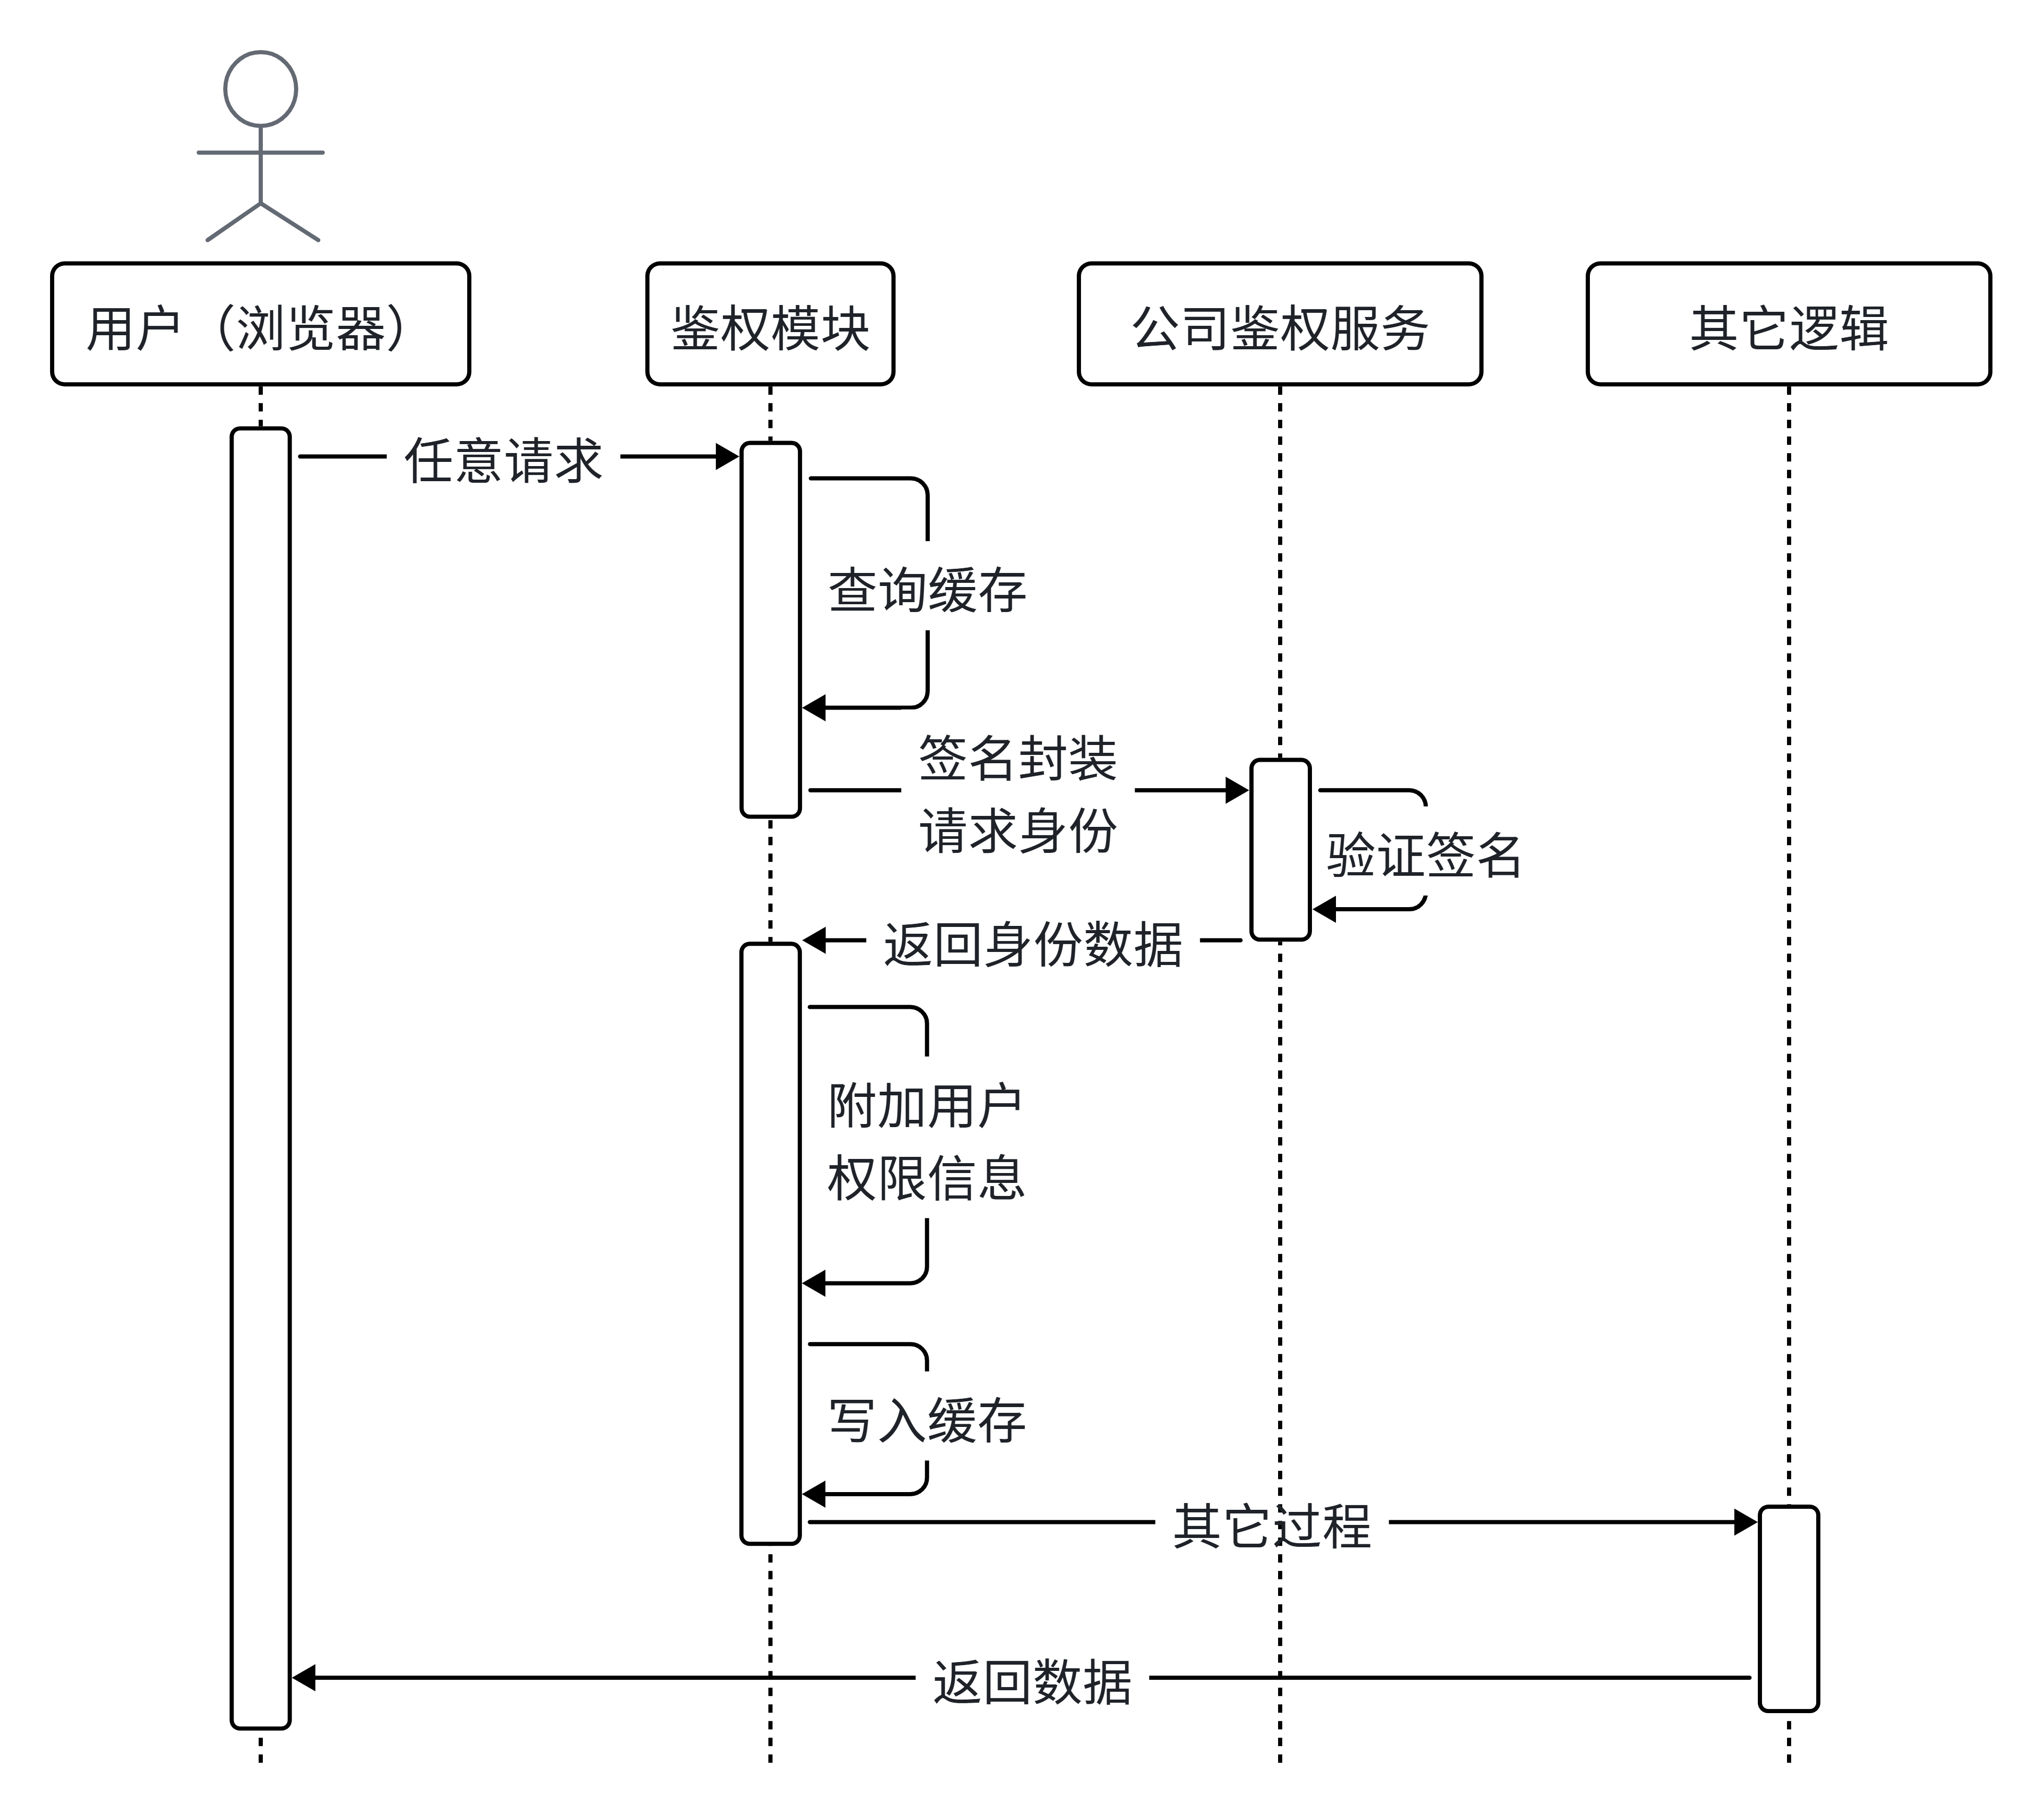
\includegraphics[width=\linewidth]{figures/4/身份认证流程.png}
    \caption{身份认证时序图}
    \label{fig:enter-label}
\end{figure}

首先，系统接收外部传入的请求，进入处理环节后，第一步是解析请求里包含的身份相关参数，这些参数是后续身份验证的基础；接着，利用解析出的参数向公司认证服务器发起请求，借助认证服务器的校验能力，获取到关于请求来源的准确身份信息；最后，把获取到的身份信息整合到原始请求的数据内容里，使后续业务处理流程能基于包含完整身份信息的请求开展，保障业务逻辑中对身份维度的需求，规范且有序地完成从请求接入到身份信息准备就绪的过程。

权限判定模块则是用于判断某个用户是否有权限操作本任务组。权限判定需要基于身份认证提供的用户信息，所以安排在身份认证之后。权限判定以一个独立部署的微服务的形式服务于本系统，有自己的前后端，结构如图4.3所示：

\begin{figure}[htbp]
    \centering
    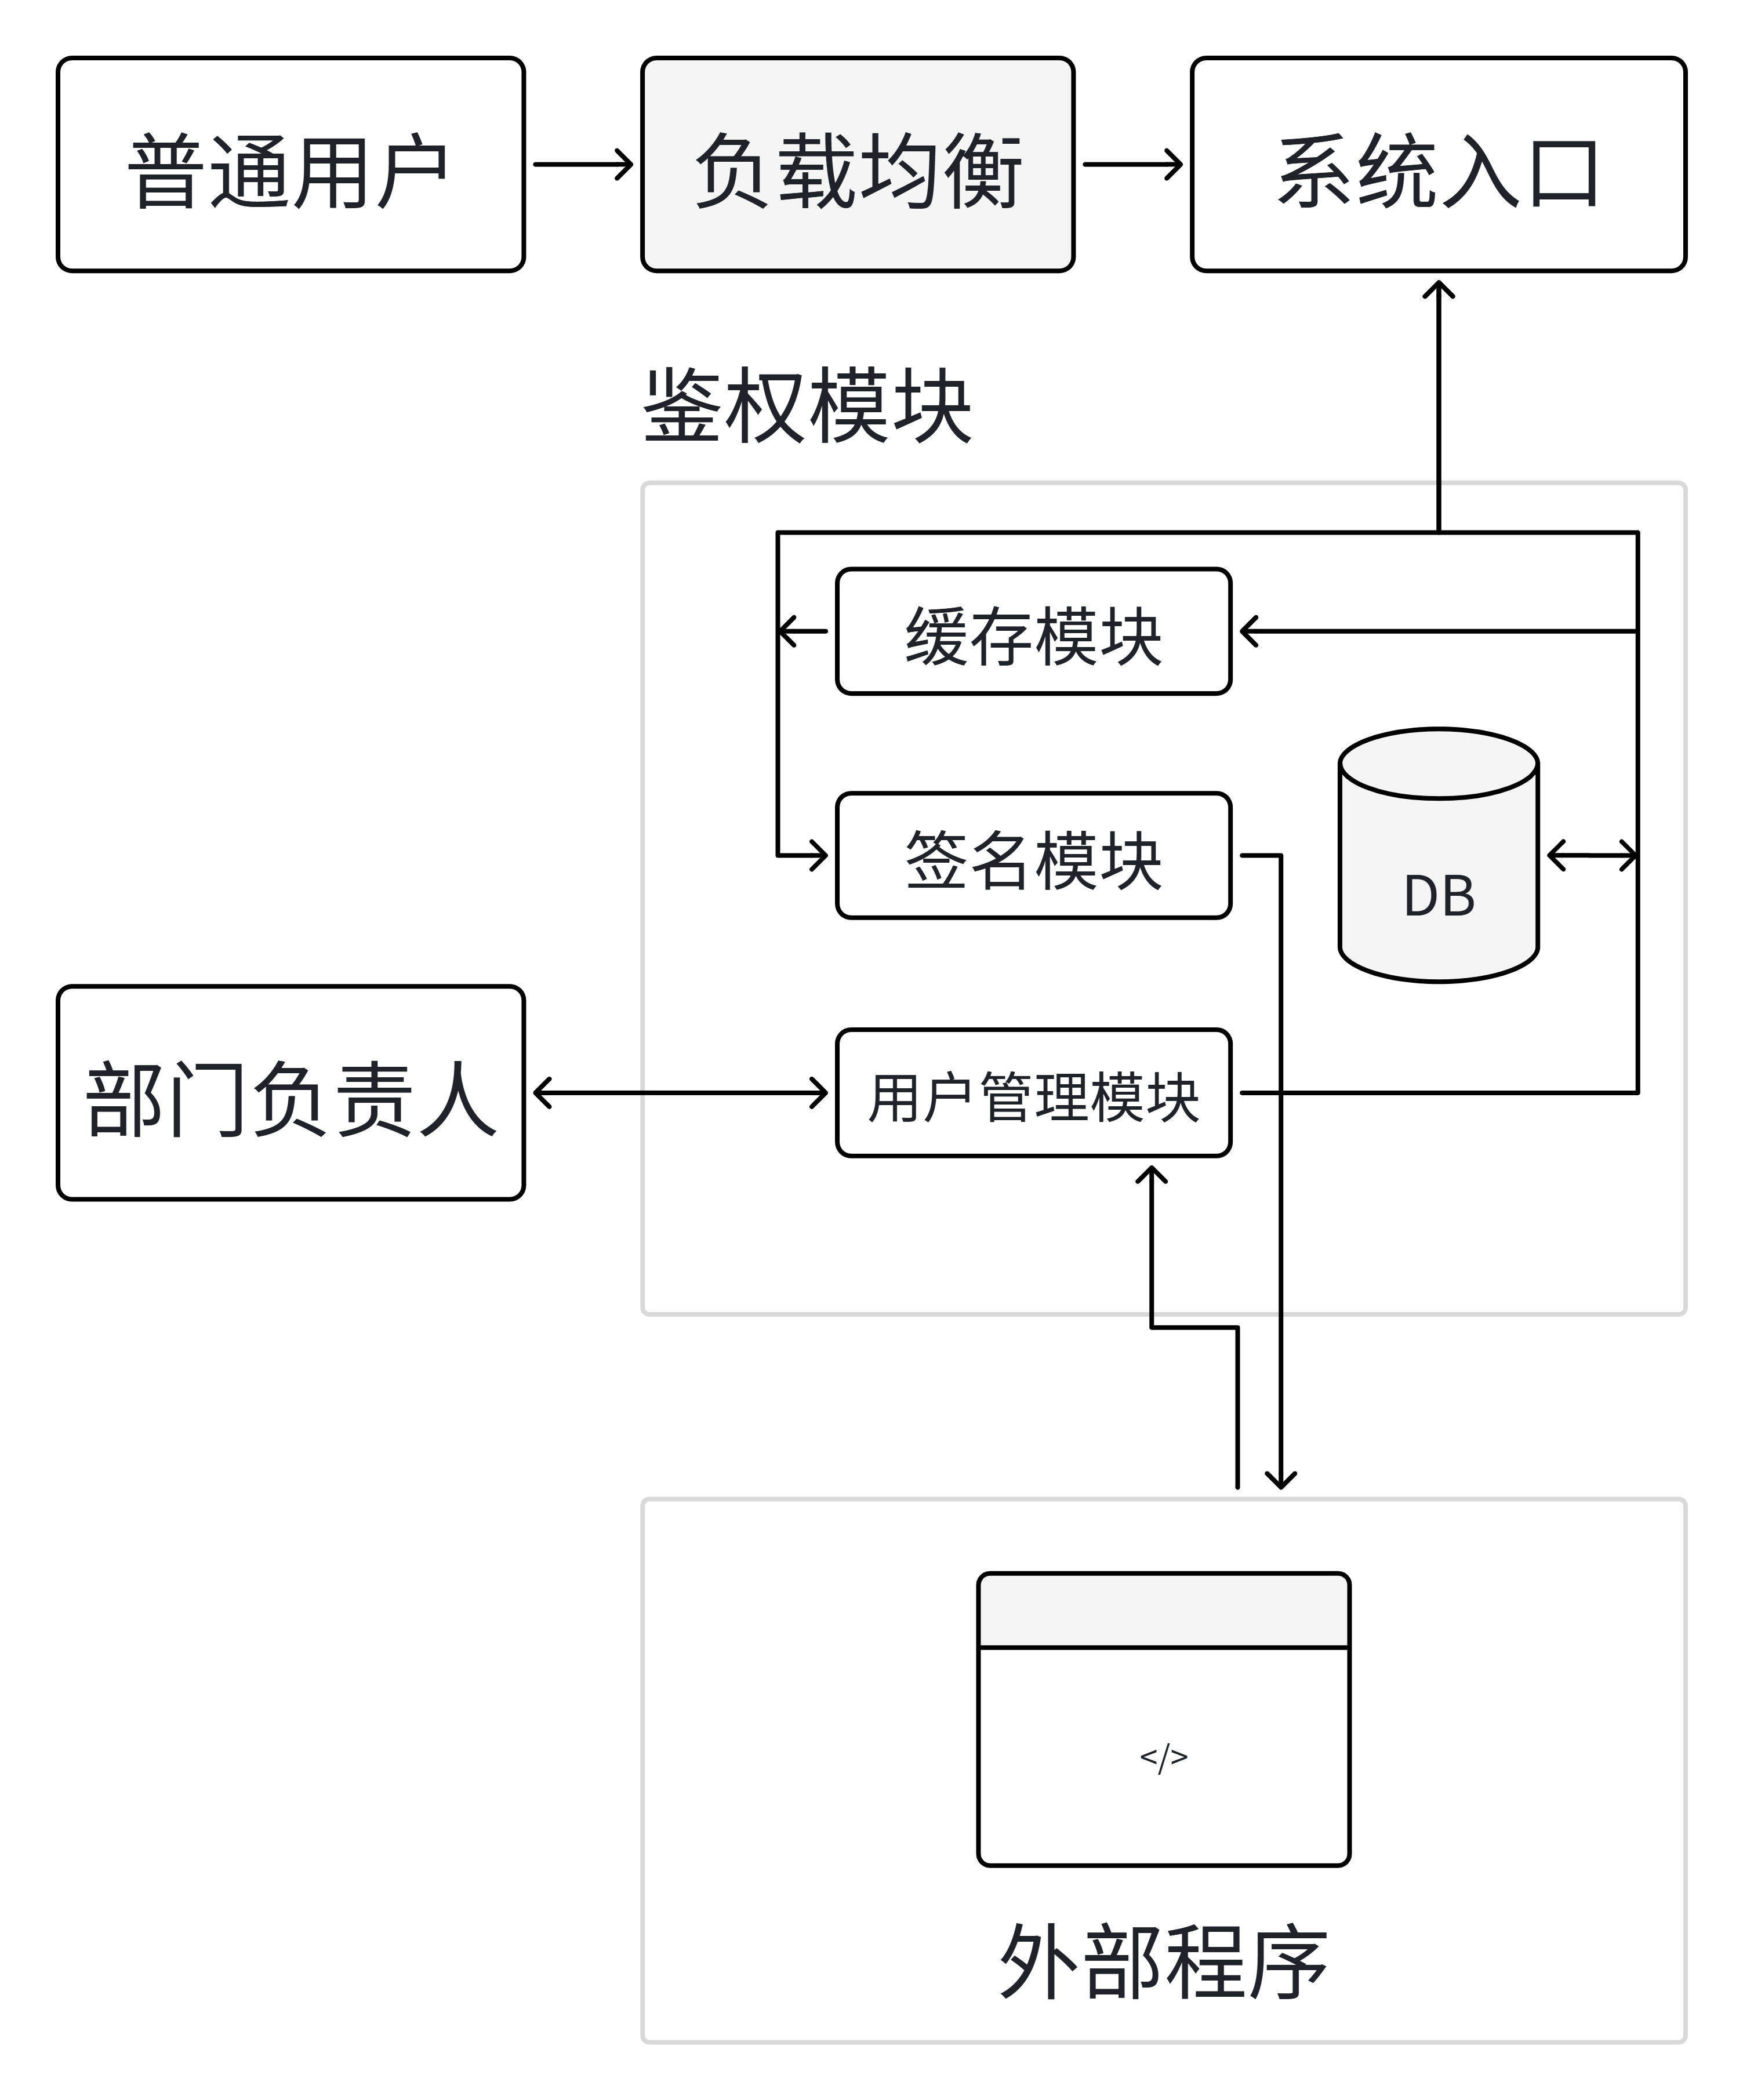
\includegraphics[width=0.6\linewidth]{figures/4/鉴权服务架构图.png}
    \caption{鉴权服务架构图}
    \label{fig:enter-label}
\end{figure}

部门负责人通过网页操作触发鉴权系统Web端，或由其他服务发起，均以HTTP请求形式传递至鉴权服务器 。鉴权服务器先经 “HTTP请求处理” 模块接收请求，再联动 “用户管理模块”与“签名验证模块”开展身份校验逻辑，过程中通过TCP协议与数据库服务器的PostgreSQL交互，查询、验证用户数据，以此实现对各类请求的鉴权管理，保障系统访问安全与权限合规。

\subsection{数据校验模块}

Pydantic是一个用Python编写的数据验证和设置管理库，基于Python的类型注解来进行数据验证等操作，在数据处理和API开发等场景中被广泛应用。本系统采用Python生态内的Pydantic库来对请求数据结构进行初步的校验。在本系统的数据结构定义层，设有一个特定目录，专门用于存放HTTP请求数据结构的定义内容。对于每个请求，均有相应的类来记录请求数据格式与响应数据格式。此外，还存在一些通用的基本结构，这些结构为所有请求和响应提供基础的数据表单。本系统以FastAPI中间件的形式，将Pydantic注册进来，以此实现无感的数据类型校验。

\subsection{业务模块}

本系统构建了以任务、统计、附件、任务组及用户为核心的五类业务API，旨在实现AI任务全生命周期的精细化管理。各API模块通过双向交互保障数据库的一致性，并深度联动鉴权模块实现细粒度的操作授权。

在底层调度逻辑上，系统利用FastAPI异步框架配合定时任务入池，依托Redis作为消息中间件（Broker）驱动Celery分布式架构。这一设计为自动化决策判断与资源互斥智能分析提供了高性能的任务分发底座。任务经由Celery Worker执行后，其进度与结果通过反向流转机制实时更新至数据库并反馈至操作面板，从而形成了从指令下发到状态回收的完整自动化业务闭环。

\section{任务调度层概要设计}

本小节着重描述和任务调度、逻辑计算相关的设计。平台收到来自前端的任务请求时，会先生成一个任务表单，加进任务池中。任务池本质上是数据库中的一个表，每个任务有自己的参数和状态。处于“等待”状态的任务会被调度模块定期检查，符合任务执行条件（任务可用、资源不冲突）时，就会加入任务队列中。同步模块负责监控任务执行程序，定期拉取处于“执行中”任务的状态，将状态写入任务池（数据库），显示到网页里，供操作员参考。

\subsection{任务可用性检测机制}

“任务可用性”是对AI任务在特定时空背景下执行合规性的多维度评估。针对调度决策过度依赖人工经验的痛点，本系统构建了基于环境感知策略驱动的逻辑引擎，旨在实现调度流程的去人工化。该机制的核心在于业务策略与调度逻辑的深度解耦。系统通过以下流程实现自动化准入控制：

\begin{enumerate}
    \item 策略配置与解析：管理员通过配置平台动态维护基于JSON格式的策略描述文件。该文件定义了涵盖任务优先级、实时系统负载阈值、特定时间窗口限制及业务场景约束等关键指标。
    \item 动态映射：系统实时监测并读取配置平台下发的JSON格式策略文件。在解析过程中，引擎并非简单的字符串匹配，而是将JSON格式的抽象策略描述精准映射为系统内部可直接调用的可计算逻辑算子。每一个配置项都会被实例化为一个具备逻辑判定能力的算子对象，这些对象按照预设的逻辑拓扑结构进行组织，最终在内存中构建出一套高性能的动态规则库。
    \item 实时准入判定：当任务处于“待调度”状态并进入决策周期时，逻辑引擎会自动触发判定流程。通过规则引擎内部的布尔演算，系统能够自主、快速地判定该任务当前是否具备启动条件。若判定结果为真，则立即下发执行指令；若环境指标触碰“熔断”红线，任务将自动保持在等待队列中。
    \item 调度闭环管理：对于判定为不满足执行条件的任务，系统将其自动置入高可靠等待队列。调度器将持续轮询环境状态，直至满足策略要求后自动触发执行。
\end{enumerate}

通过这种“策略驱动”的自动化机制，系统有效消除了传统调度模式中对人工干预的依赖，在保障系统运行平稳的同时，显著提升了多任务并发场景下的决策效率。

\begin{figure}[htbp]
    \centering
    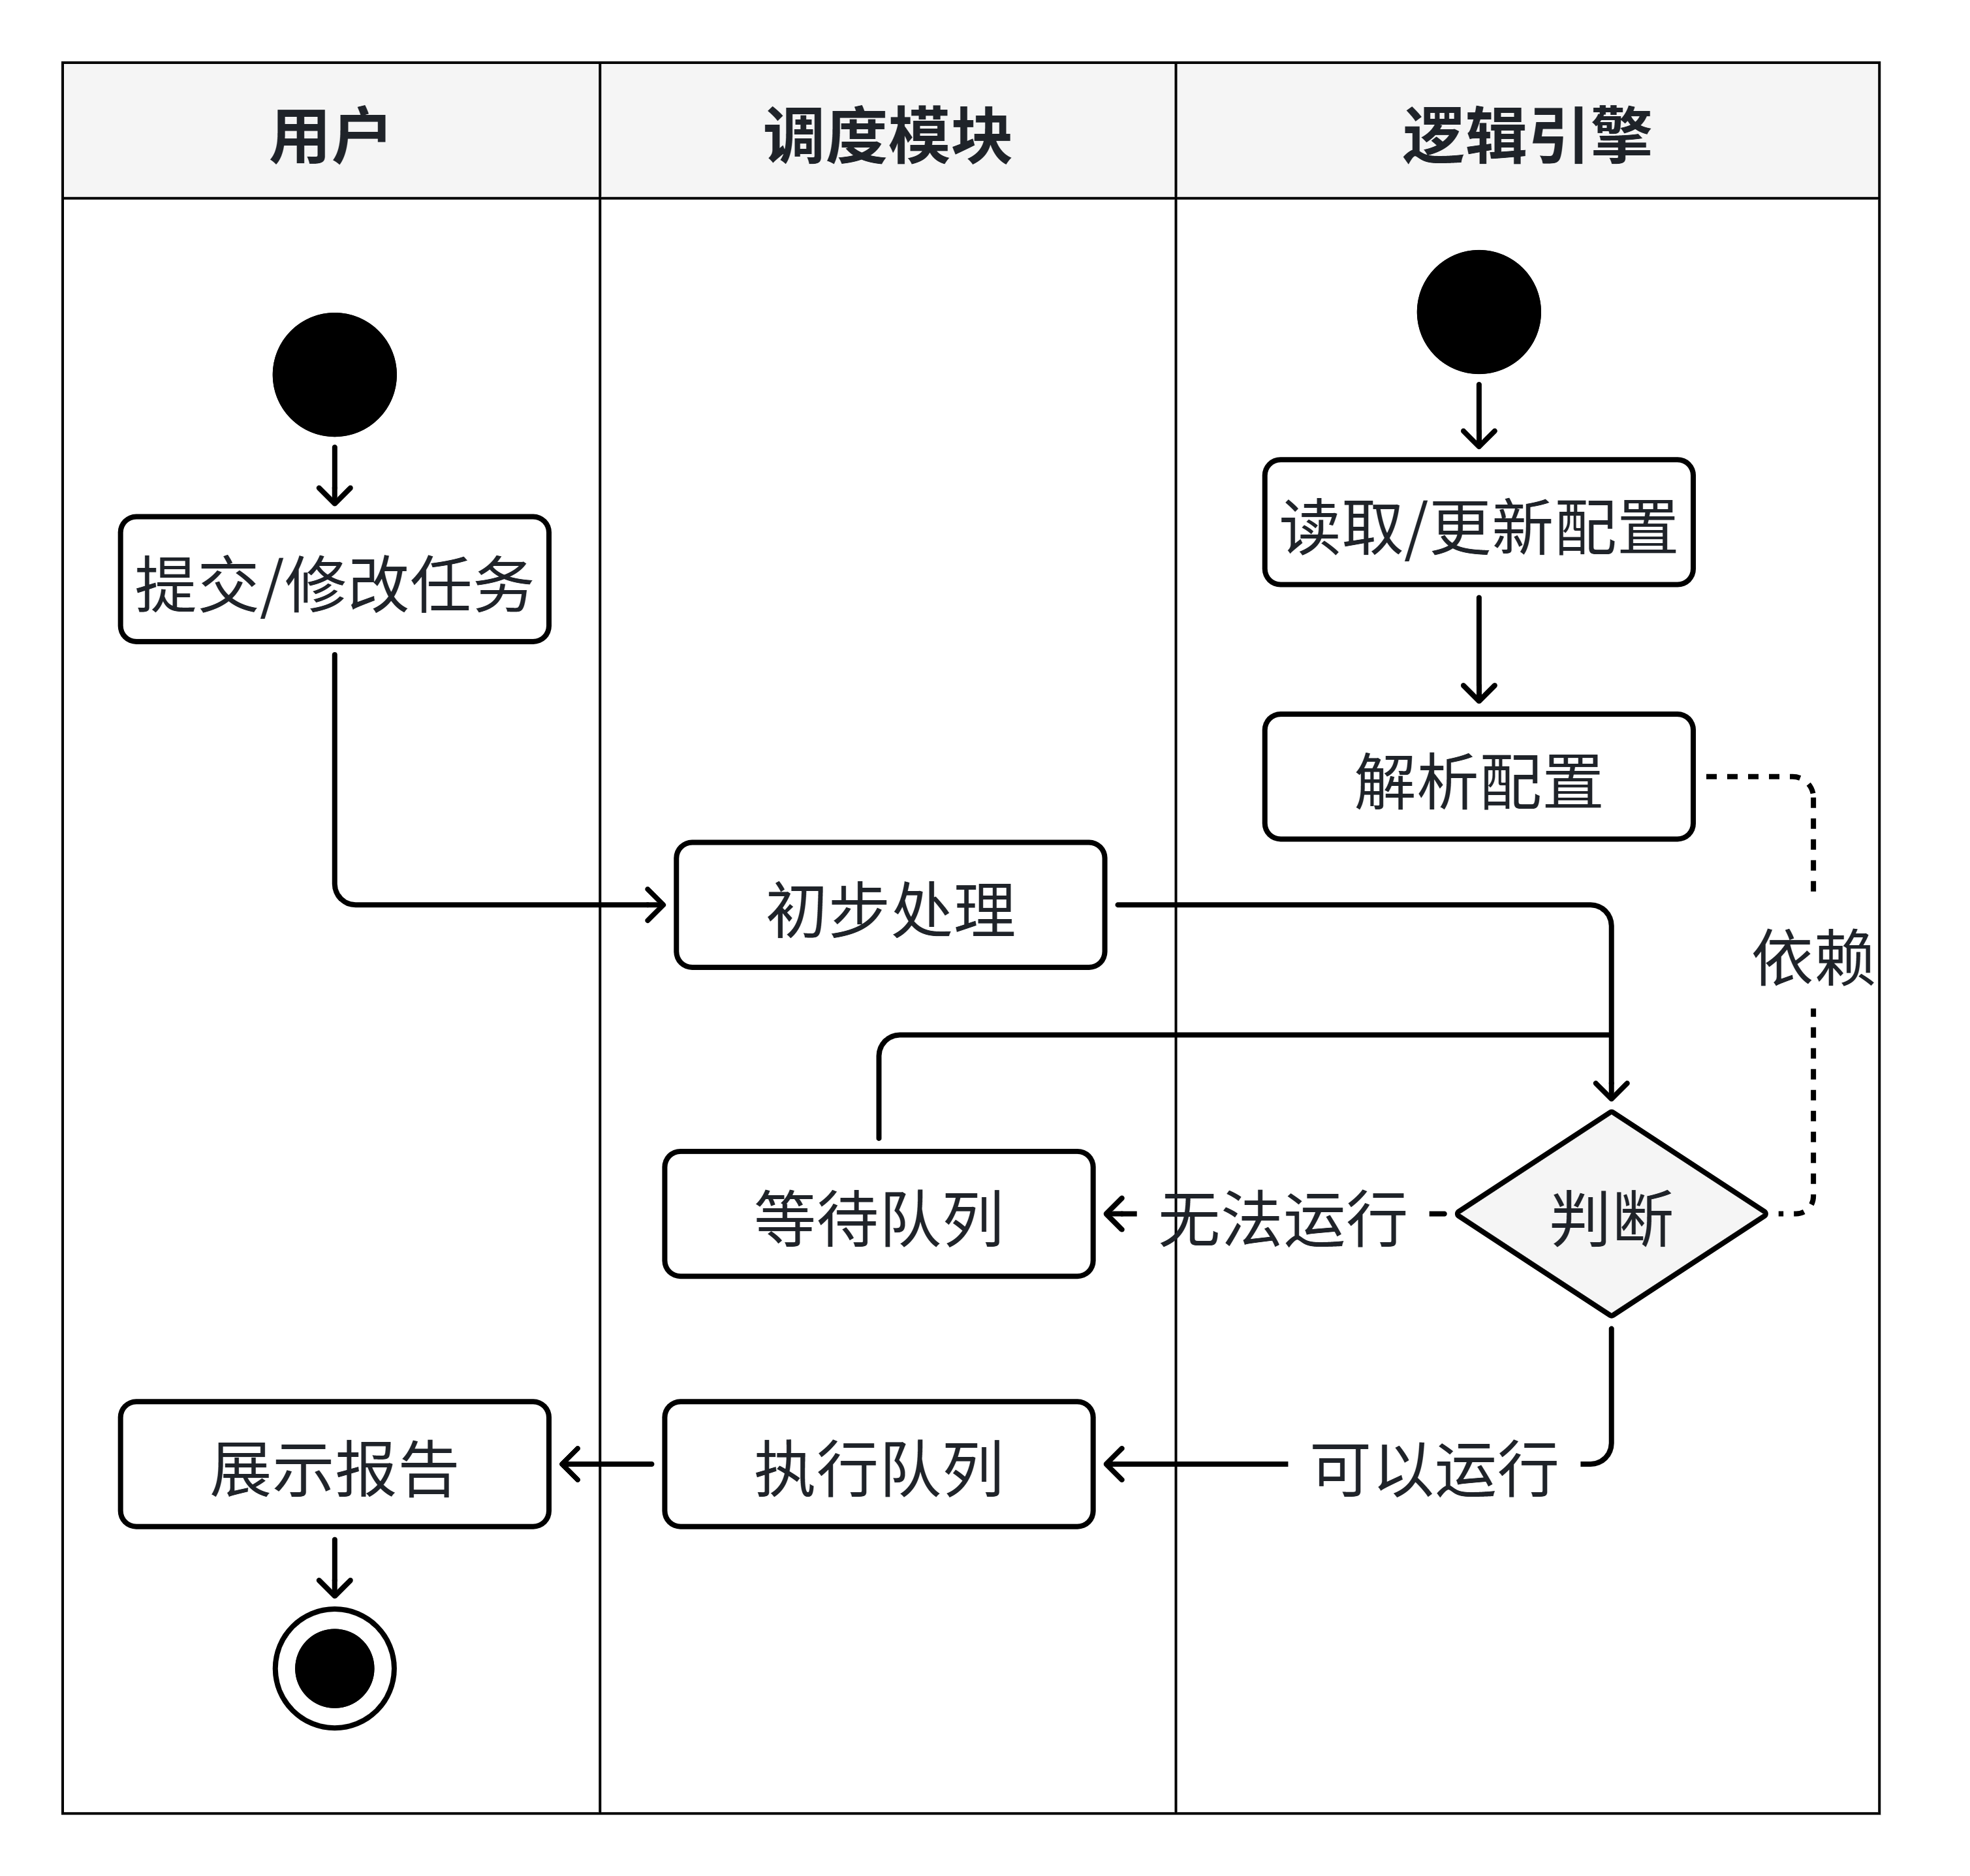
\includegraphics[width=0.8\linewidth]{figures/4/任务可用性判断流程图.png}
    \caption{任务可用性判断泳道图}
    \label{fig:enter-label}
\end{figure}

任务可用性判断流程如图4.4所示。当用户通过操作面板提交或修改任务请求后，调度模块首先执行基础的参数预处理，随后将其透传至逻辑引擎进行准入判定。逻辑引擎基于预解析的规则库，结合任务特征与当前系统环境约束，自主决定任务的执行时机：若判定为“无法运行”，任务将进入等待队列挂起，直至满足条件后被自动唤醒；若满足条件，则分发至执行队列并向用户展示反馈报告。该流程实现了从“人工干预”向“引擎自决”的转变，是提升调度自动化水平的关键环。

\begin{figure}[htbp]
    \centering
    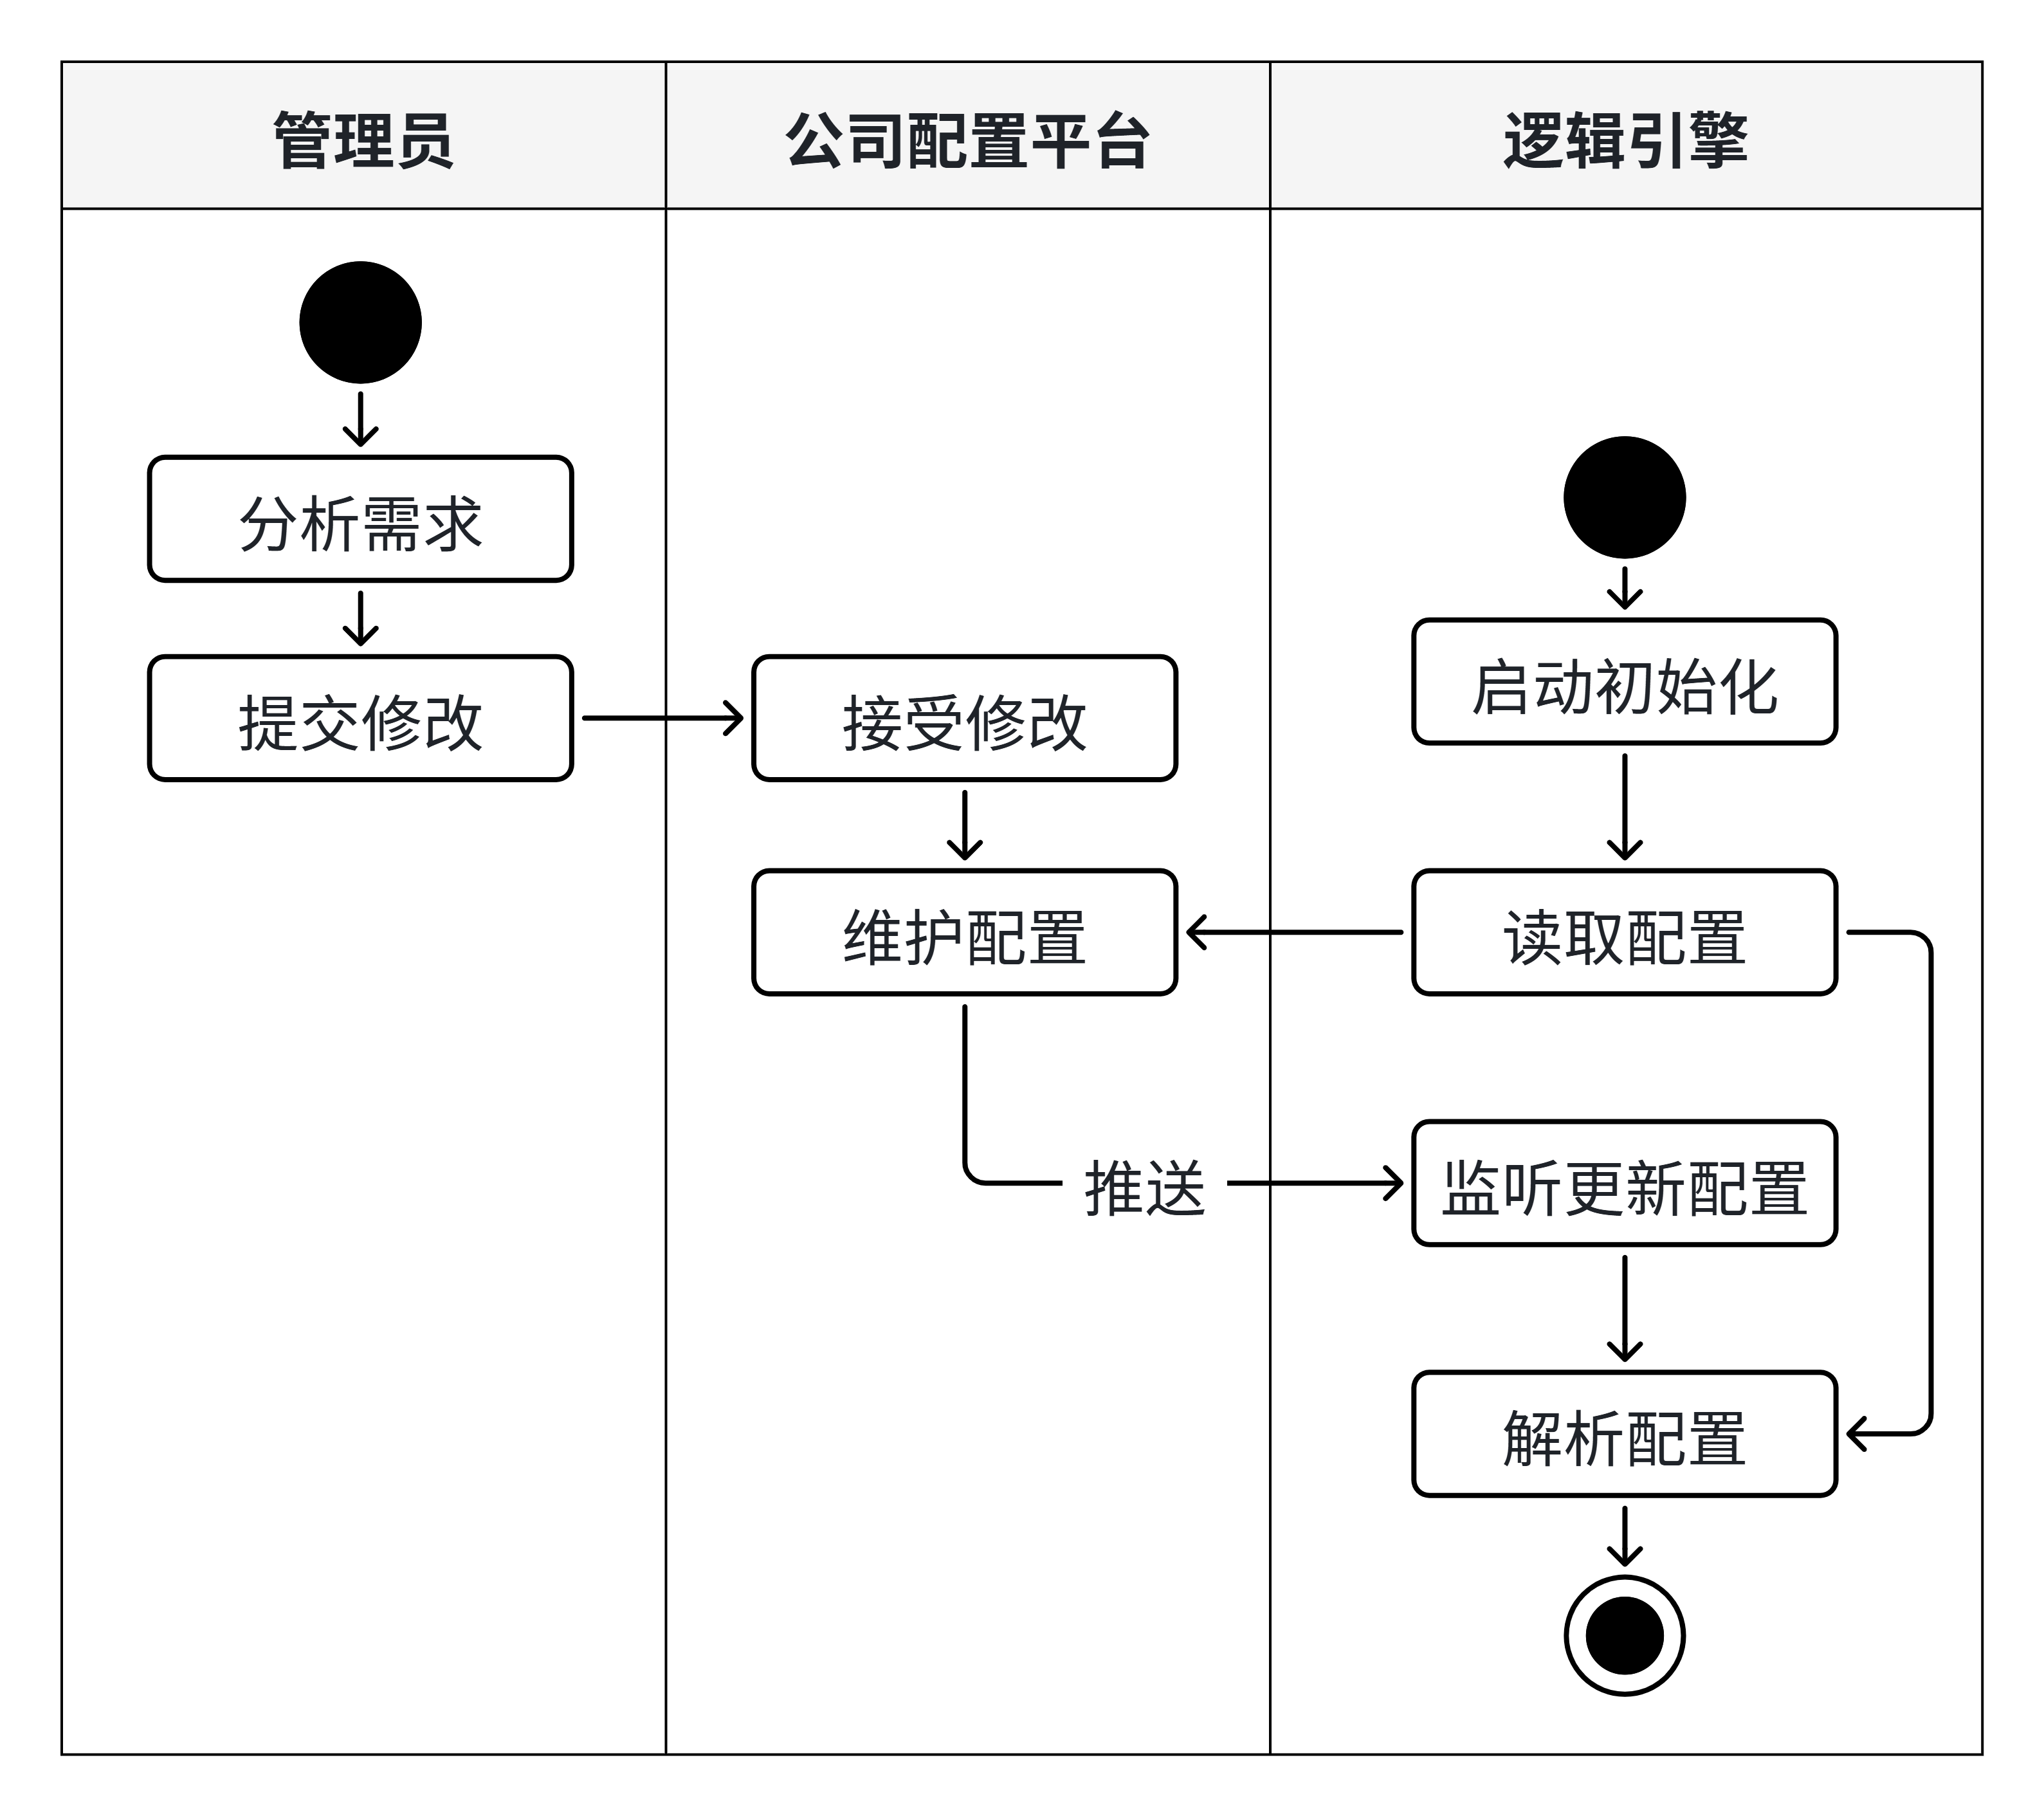
\includegraphics[width=0.8\linewidth]{figures/4/规则配置流程图.png}
    \caption{规则配置泳道图}
    \label{fig:enter-label}
\end{figure}

规则配置流程如图4.5所示。系统通过管理员在公司配置平台的策略修订实现逻辑规则的动态演进。平台接收修改请求并完成维护后，通过推送机制与逻辑引擎实现同步。逻辑引擎在启动初始化阶段完成既有配置的读取，并在运行期通过持续监听机制捕获动态更新指令，确保能够即时解析最新的策略文件并映射为可执行逻辑。该机制保障了调度策略的灵活性，使得系统能依据实时负载（如系统负载阈值）或特定业务约束，精准调控AI任务的准入状态。

\subsection{资源可用性检测机制}

针对计算资源互斥导致的任务串行与算力空耗难题，系统构建了精细化的算子资源管控体系。AI任务的运行高度依赖底层计算资源，其中CPU与内存多采用操作系统的抢占式调度策略，而GPU等高性能算力资源在执行大模型推理或训练时，通常表现为强独占性的临界资源。若系统缺乏对临界资源的感知能力，导致多个任务并发竞争同一物理GPU节点，将不可避免地引发显存溢出、数据冲突或执行失败等问题。为解决这一瓶颈，本系统设计并引入了“临界资源表”及其配套的冲突分析逻辑：
\begin{enumerate}
    \item 资源状态跟踪：系统通过临界资源表实时维护任务与资源的动态映射关系，记录资源占用状态等详细信息。该表可关联并锁定多个异构资源标识，从而实现对全局算力占用情况的精准捕获。
    \item 并发冲突判定：调度引擎在任务下发前，会检索临界资源表以识别目标资源是否处于锁定状态。通过这种资源拓扑识别机制，系统能够精准区分“可并发任务”与“互斥任务”，从而打破传统模式下盲目串行执行的限制。
    \item 动态分配与释放：系统根据资源表的反馈进行决策，若检测到冲突则将任务延时调度，若资源空闲则即时锁定并分配。
\end{enumerate}

通过该机制，系统实现了对算力资源的闭环管理，在保障AI任务执行安全性的同时，显著提升了集群的并发吞吐量与资源周转效率。

\subsection{负载均衡及性能优化设计}

为应对任务量增长以及需求的不断膨胀，本系统采用了可灵活扩展执行器的结构设计。然而，受预算及设备类型的限制，不同执行器节点的计算能力存在差异，进而致使其执行能力参差不齐。

本系统设计了一套调度机制，能够合理地将任务分配至不同节点。其中，系统借鉴了C语言编写的高性能HTTP服务器NGINX中用于处理动态负载均衡的权重轮询（Weighted Round Robin）算法。该算法主要用于处理动态负载均衡部分主要负责操作服务器的权重数据和向目标服务器转发客户的请求。此部分是在upstream机制中的加权轮询算法的基础上优化得到的\cite{10}。基于此，本系统实现了一个简化的权重轮训机制。每台执行机都配置有由管理员设定的权重。任务调度器依据这些权重，将任务分配至各台执行机。在分配任务之前，调度器会首先查询执行机的状态。若某台执行机处于满载状态，调度器便会跳过该机器。倘若所有执行机均处于满载状态，调度器则会跳过此次任务，而被跳过的任务将会等待下一次调度。

\subsection{数据同步模块}

本系统多个模块独立部署在不同的计算机系统上，彼此间有通信和数据同步需求。HTTP接口层与任务调度器通过 “任务池” 的形式实现任务同步。接口层在对任务参数与运行环境进行初步处理后，会把任务信息写入单独部署的数据库。任务调度器（其部署位置可能与接口层在同一台机器，也可能不同）从该数据库中提取处于特定状态的任务，并在恰当的时机将这些任务发送至Celery的任务队列。与此同时，任务调度器还会定时从Celery的结果队列中获取正在执行任务的相关信息，将任务的进度或结果写入数据库，最终这些信息会展示在网页上。执行器使用Celery执行端来接收Redis任务队列数据库中的任务数据，并定期将任务的进度条信息写入Redis的结果队列数据库。系统选用Redis作为消息队列，以满足 “管理平台程序”与 “执行器集群”之间的数据互通需求。在本系统中，会运用Redis的两个数据库（DB Number），分别专门用于任务的发送与接收。Redis的核心逻辑基于单线程运行，这一特性使得即便无需考虑任何并发锁设计，本系统也能够有效地避免任务的重复发送与重复消费。此外，Redis借助TCP协议进行数据传输，这进一步保障了任务信息不会丢失。

\subsection{容错与恢复机制}

本系统采用微服务架构。在这种架构下，不同服务间可能因版本更新不及时，引发数据传输问题，例如出现参数类型混淆，像float与int类型被错误混用的情况。此外，部分参数由操作员手动输入，这可能导致拼写错误或格式不符等问题。鉴于上述情况，本系统的API接口层在处理任务参数时，会针对参数中常见的基本错误进行初步纠错。纠错主要体现在以下几方面：
\begin{enumerate}
	\item 参数类型：若参数类型错误，虽能正常传递至AI任务，却会致使AI任务在执行中途出现异常，进而造成损失。基于此，本系统会先对参数类型展开初步校验与转化。只有在实在无法完成转化的情况下，才会向操作员抛出异常。
	\item 拼写错误：操作员在指定任务的部分参数时，有可能出现拼写错误。比如在填写某些列表时，可能会混淆全角与半角的逗号分隔符。针对此类情况，本系统设置了相应的恢复机制。
	\item 选择错误：当操作员做出存在矛盾的选择（比如选择在非GPU集群上运行GPU任务）时，本系统会尝试进行修正。具体而言，系统会通过办公软件向操作员提交审批申请，待审批通过后，便会自动更正参数，并将任务发送出去。
\end{enumerate}

\section{任务执行层概要设计}

面对日益增长的AI计算吞吐量，任务执行层被设计为解耦、可水平扩展的分布式算力单元。针对AI异构数据适配性欠佳的痛点，本层重点强化了执行环境的数据感知识别与鲁棒性适配。其核心功能需求通过以下三个机制实现：

\begin{enumerate}
    \item 异构环境初始化与数据映射机制：针对AI任务强数据依赖的特征，本层在初始化阶段通过参数画像匹配，实现远程附件的并发拉取与异构数据路径的本地化重定向。该机制确保了复杂AI参数在分布式执行节点间的一致性，从执行端消解了由于环境差异导致的数据处理障碍。
    \item 全生命周期监控与动态干预机制：系统需实时捕获任务在底层算力平台的运行状态。为提升运维灵活性，该机制支持任务在运行期的撤销与参数在线编辑，确保当业务逻辑或资源分配发生变更时，能即时终止旧进程并释放临界资源。
    \item 结构化结果回收与异常捕获机制：执行层负责建立高可靠的结果上报链路，对任务产出的非结构化数据及执行异常进行自动化收集与分类。通过细粒度的监控指标反馈，为上层调度中枢的决策闭环与容错恢复提供精准的数据支撑。
\end{enumerate}

\subsection{参数传递约定}

由于本系统所有组件均采用Python语言开发，组件间的参数传递统一基于Python原生数据类型。任务的启动参数采用Python字典（dict）类型，该类型内部并未设定任何硬性的格式要求。操作员注册任务并上传任务代码时，需要一并注册任务参数类型。在此之后，当启动任务时，系统的前端操作面板会自动显示与响应数据格式对应的表单，方便操作员填写。任务执行模块首先会准备任务执行所需要的参数。深度学习算法具有较强的数据依赖性，需要大量标注数据和计算资源\cite{liang2025survey}，所以这个过程还会拉取远端资源至本地临时目录，方便任务程序读取。首先程序会检查任务是否依赖远端附件。若依赖，则会向公司的COS（对象存储服务）拉取对应文件，并暂存在本系统的目录中。随后，程序会更改参数中的文件路径为本地路径，再传入任务，供任务代码读取。

\begin{figure}[ht]
    \centering
    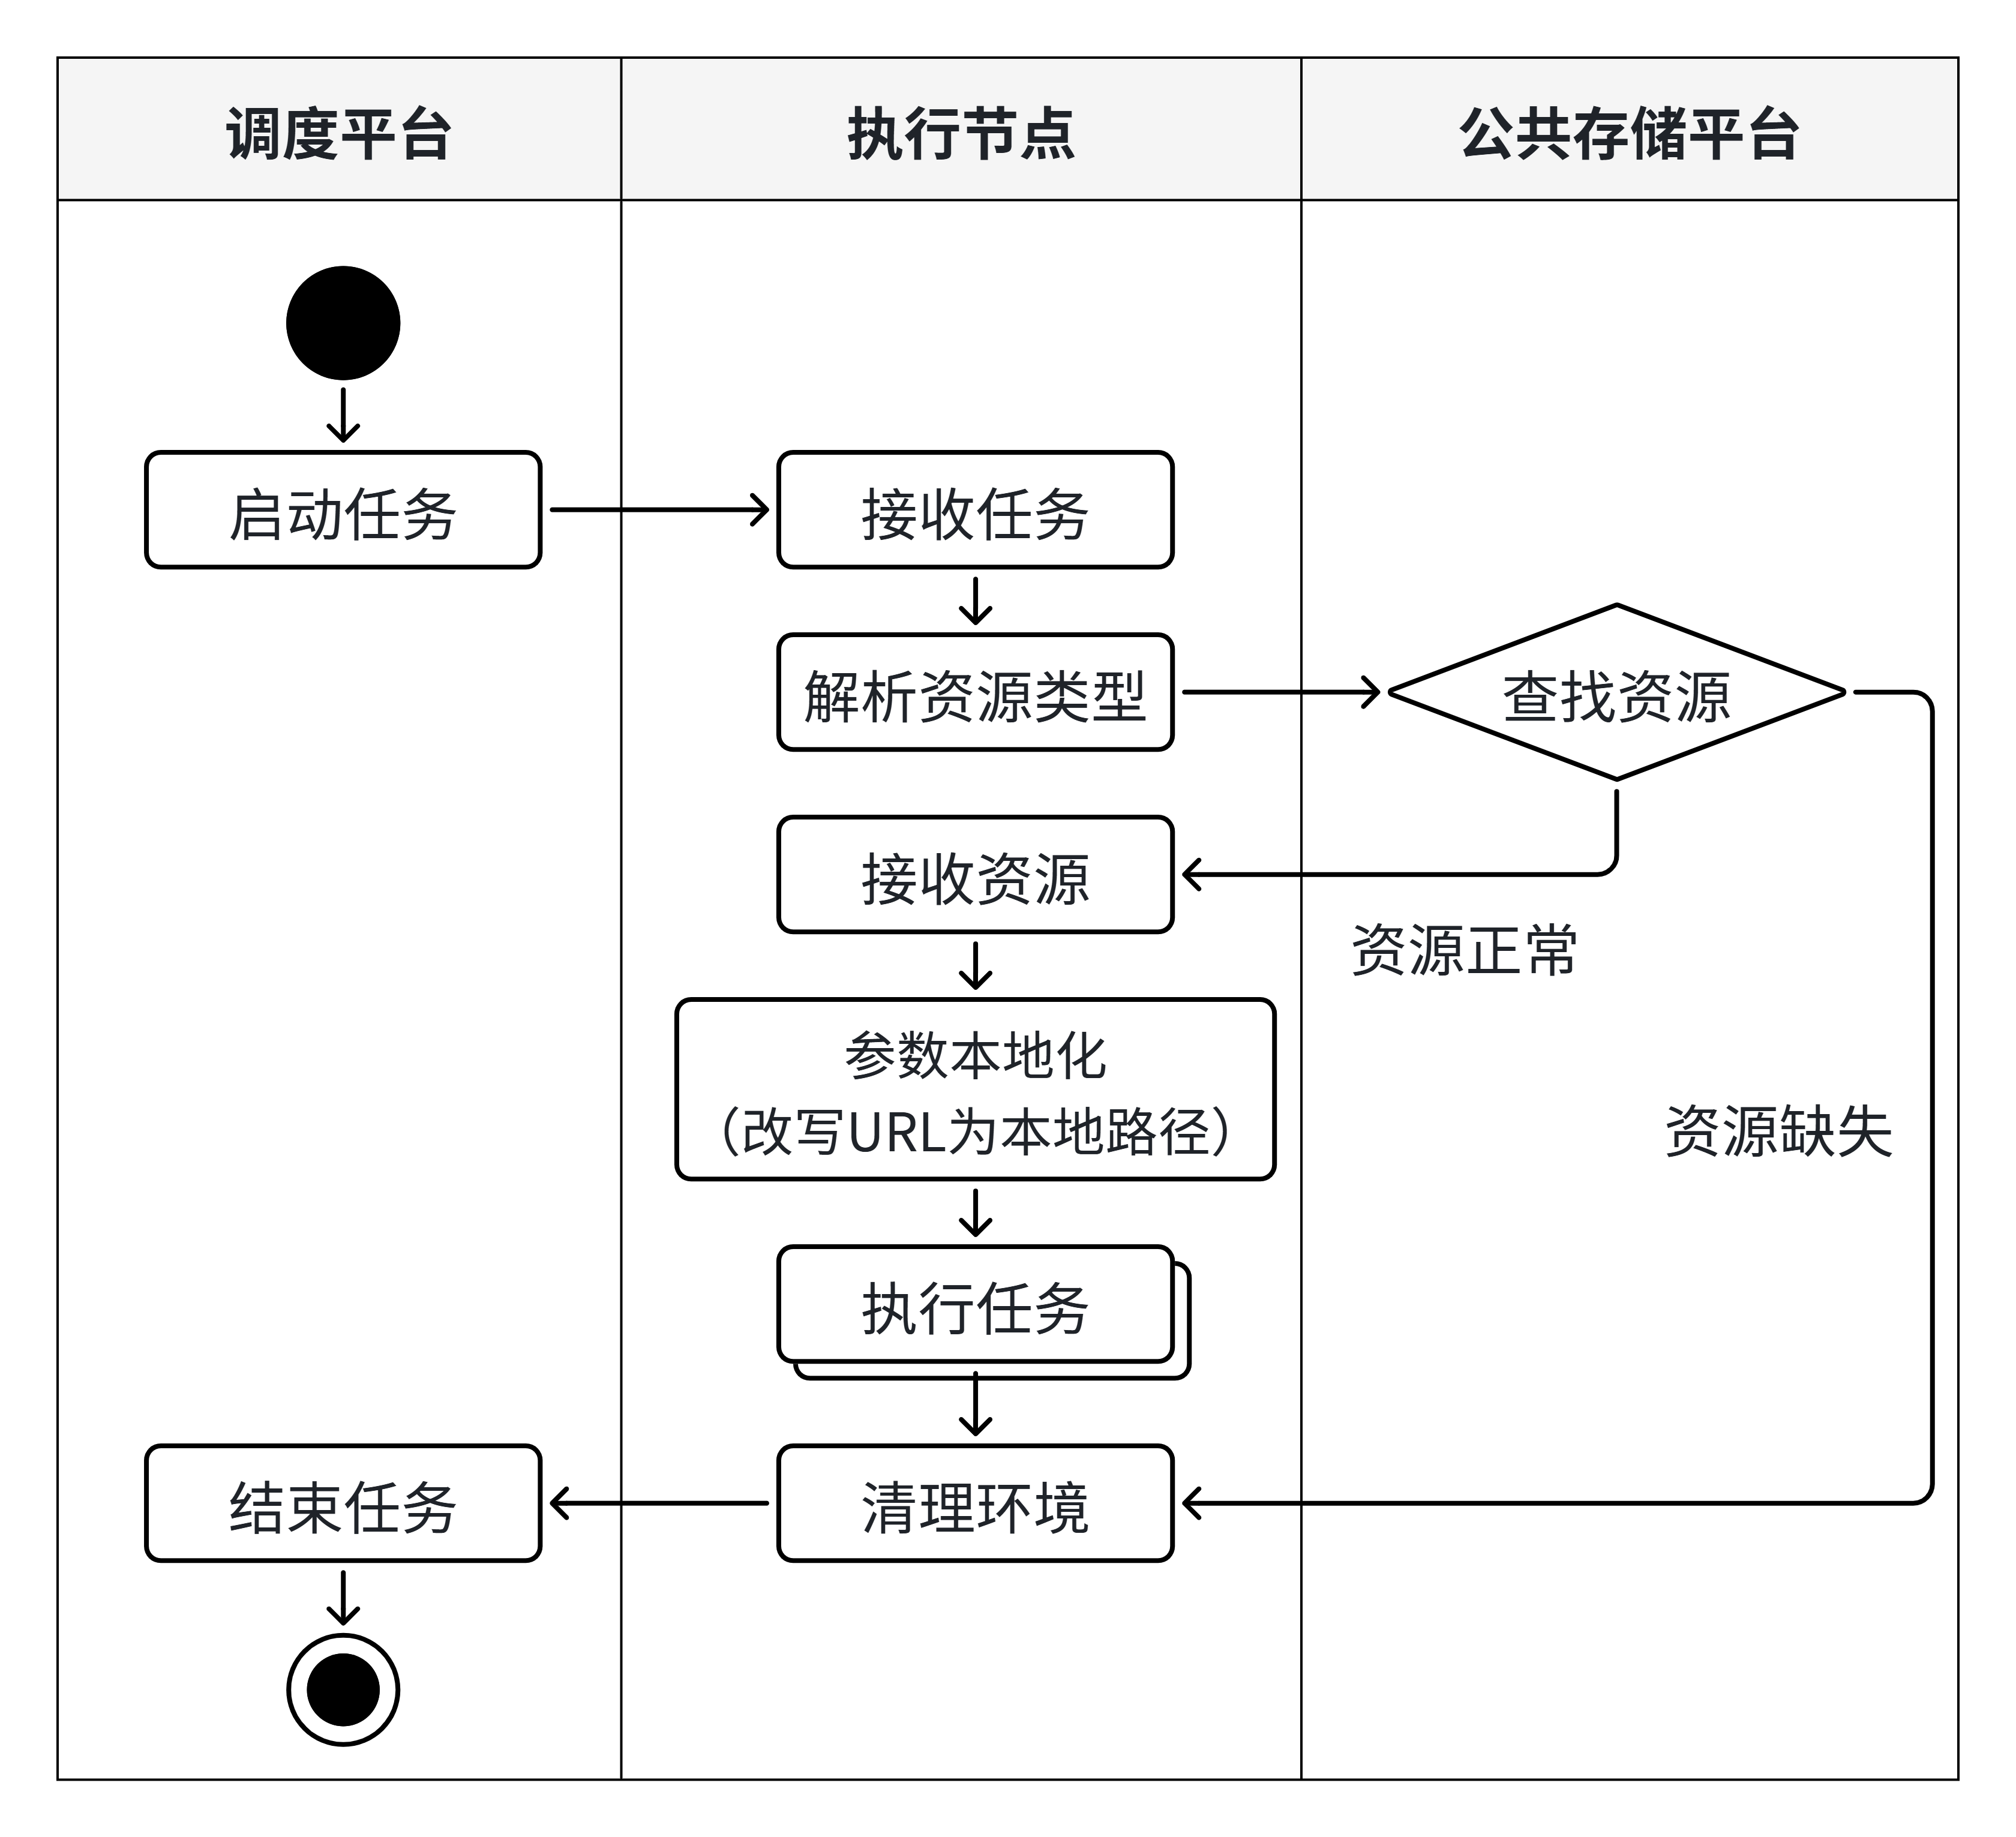
\includegraphics[width=0.8\linewidth]{figures/4/资源拉取流程图.png}
    \caption{资源拉取泳道图}
    \label{fig:enter-label}
\end{figure}

资源拉取流程如图4.6所示。

\subsection{任务编辑方式}

任务编辑机制为操作员提供了动态修正业务逻辑的途径，旨在解决因需求变动或录入失误导致的参数偏差。系统支持对处于任意生命周期阶段（等待或运行态）的任务进行在线编辑。执行编辑操作时，调度中枢首先检索任务状态：若任务正在运行，系统将立即终止其执行进程及相关子进程，从而强制释放其独占的GPU等临界资源，为后续并发调度腾出算力空间；若任务处于待发起状态，则直接进行逻辑覆盖。编辑完成后，原任务将被注销，系统依据修正后的异构参数生成新任务实例。由于参数变动可能引发新的资源互斥或策略约束，新任务将重新置于等待队列末尾，并联动自动化决策引擎重新进行准入判定。任务编辑流程如图4.7所示。

\begin{figure}[htbp]
    \centering
    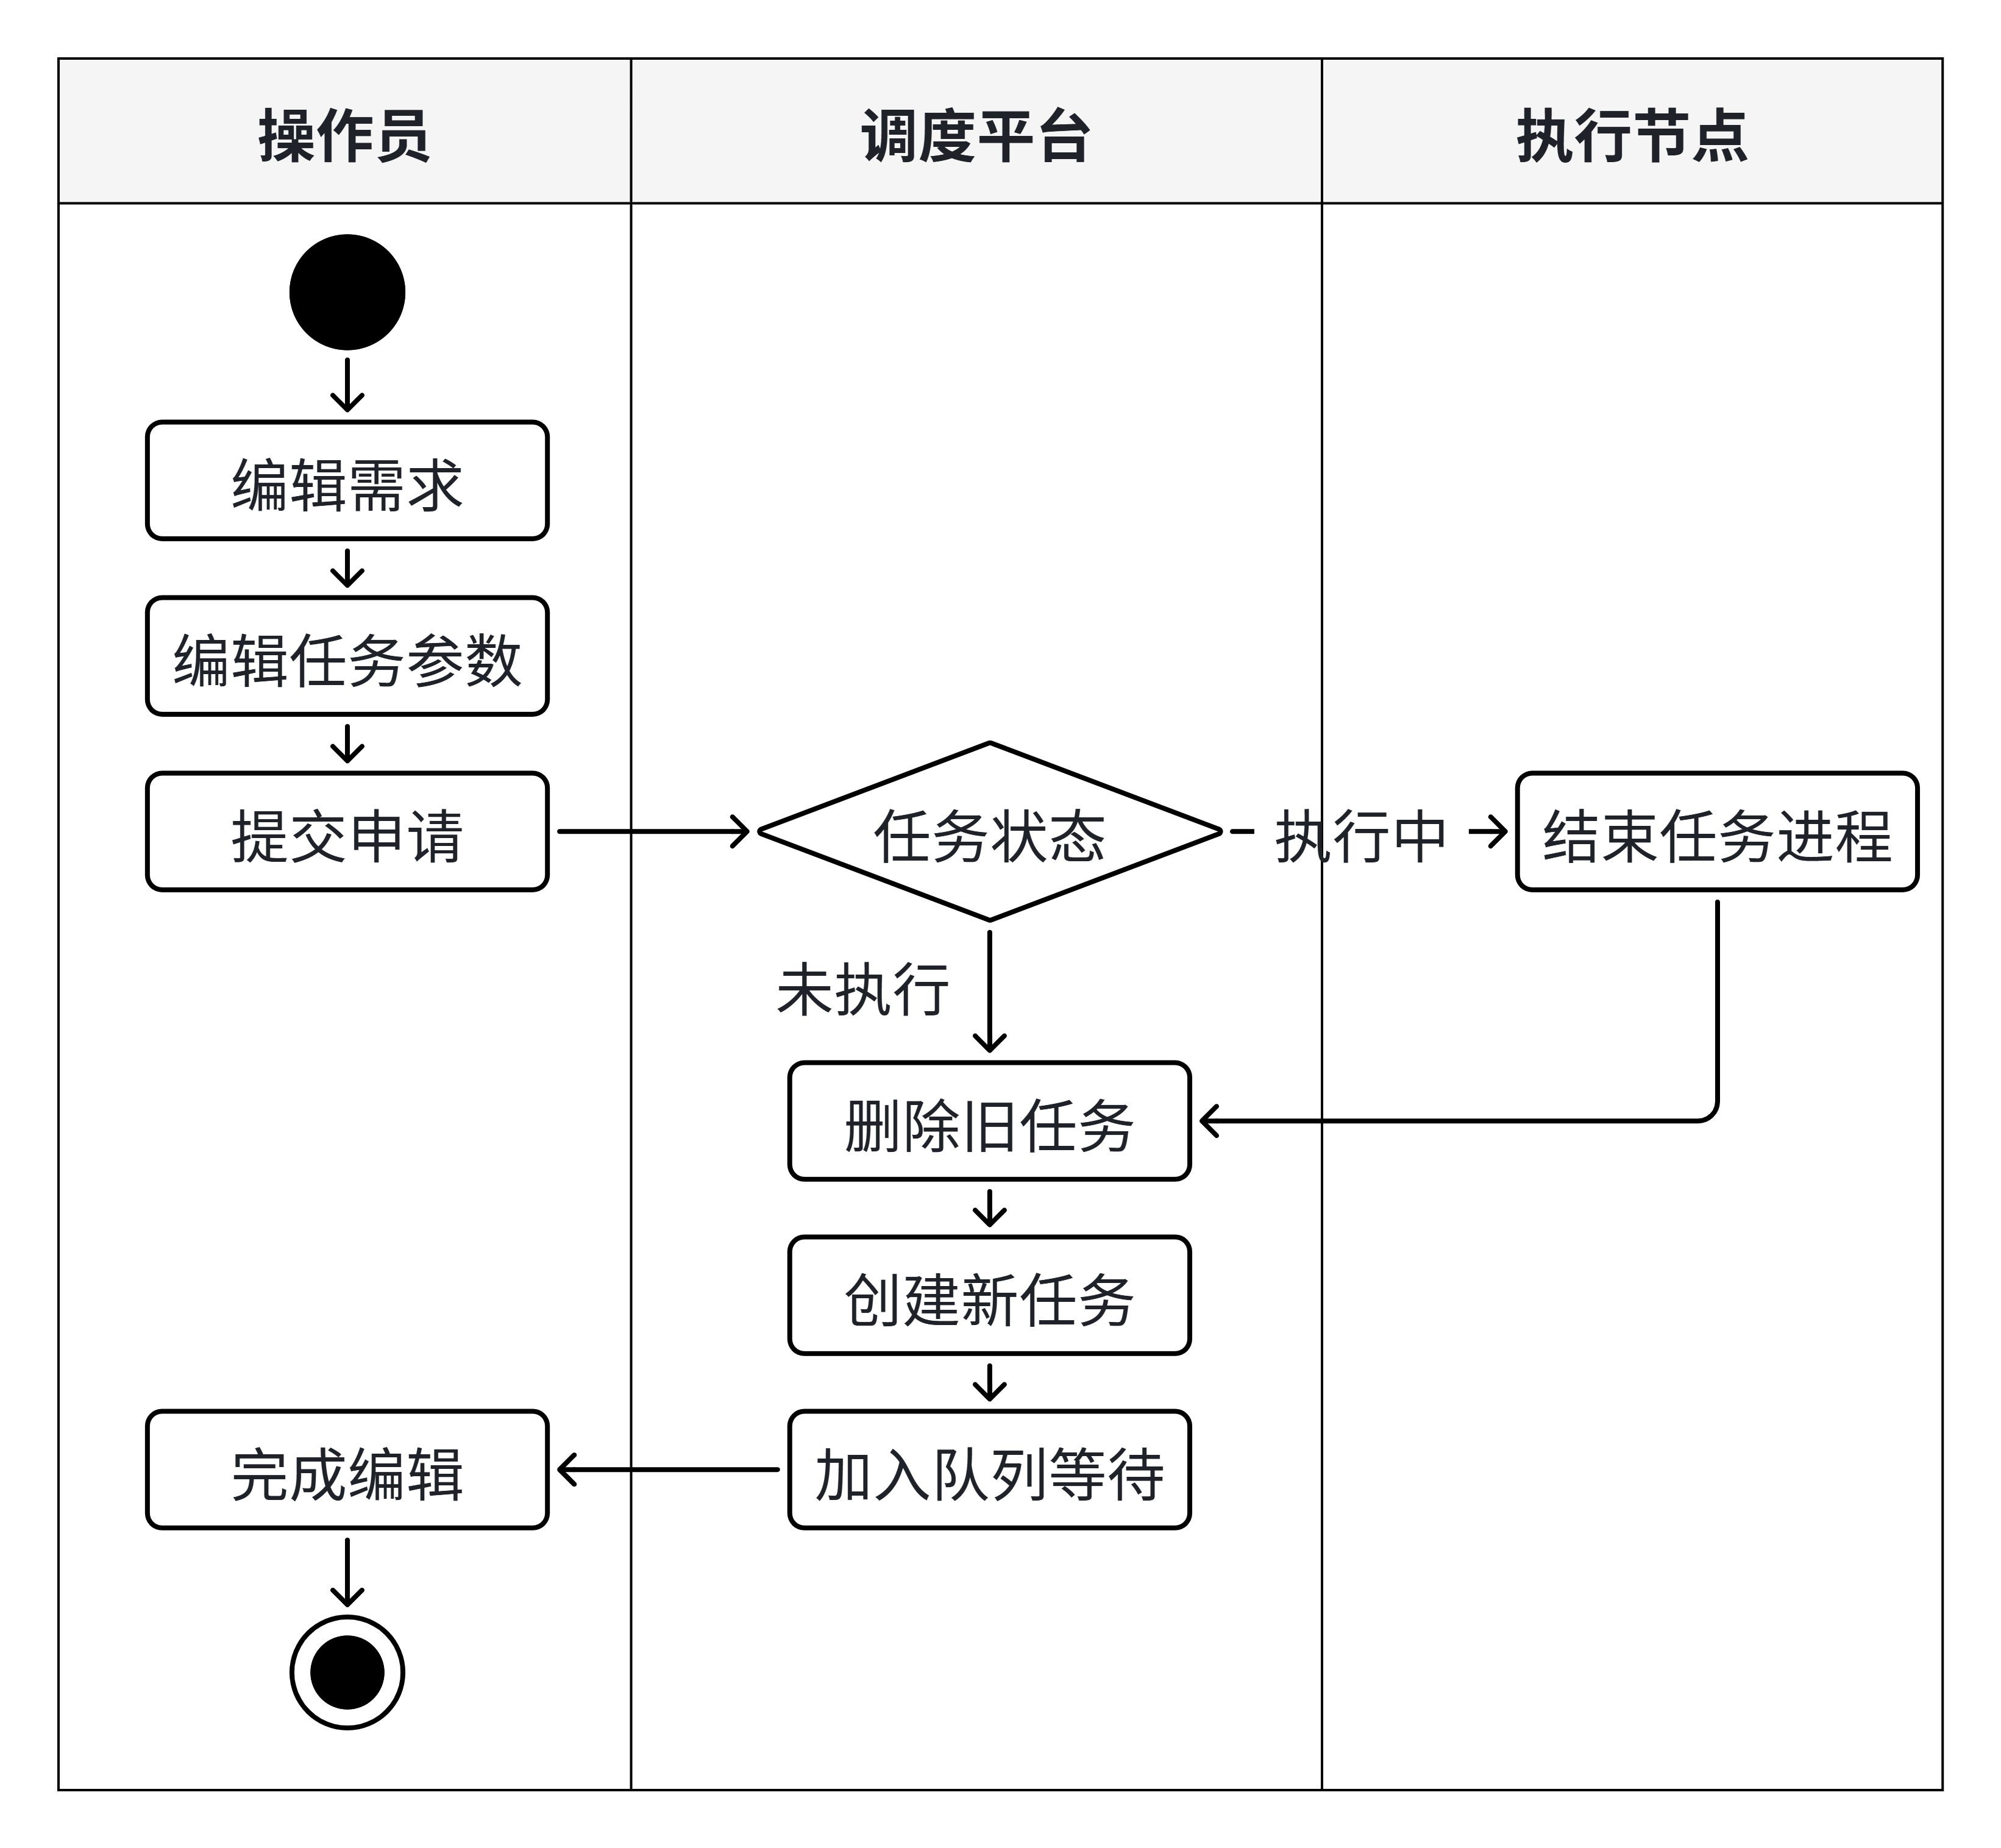
\includegraphics[width=0.9\linewidth]{figures/4/任务编辑流程.png}
    \caption{任务编辑泳道图}
    \label{fig:enter-label}
\end{figure}

任务撤销功能主要用于清理业务场景中不再需要的冗余任务，是优化系统算力周转率的重要手段。操作员可手动触发撤销指令，系统随后进入状态检查流程：对于执行中的任务，执行层将捕获撤销信号并强制关闭计算进程，即时阻断无效的算力消耗，解决资源浪费问题；对于处于等待队列的任务，系统则直接移除其元数据及关联的附件引用。撤销操作执行后，系统将从任务池中彻底剔除该实例的调度序列，并同步更新临界资源表，确保调度中枢能够基于最新的资源拓扑进行下一轮的智能并发分析。任务撤销流程如图4.8所示。

\begin{figure}[htbp]
    \centering
    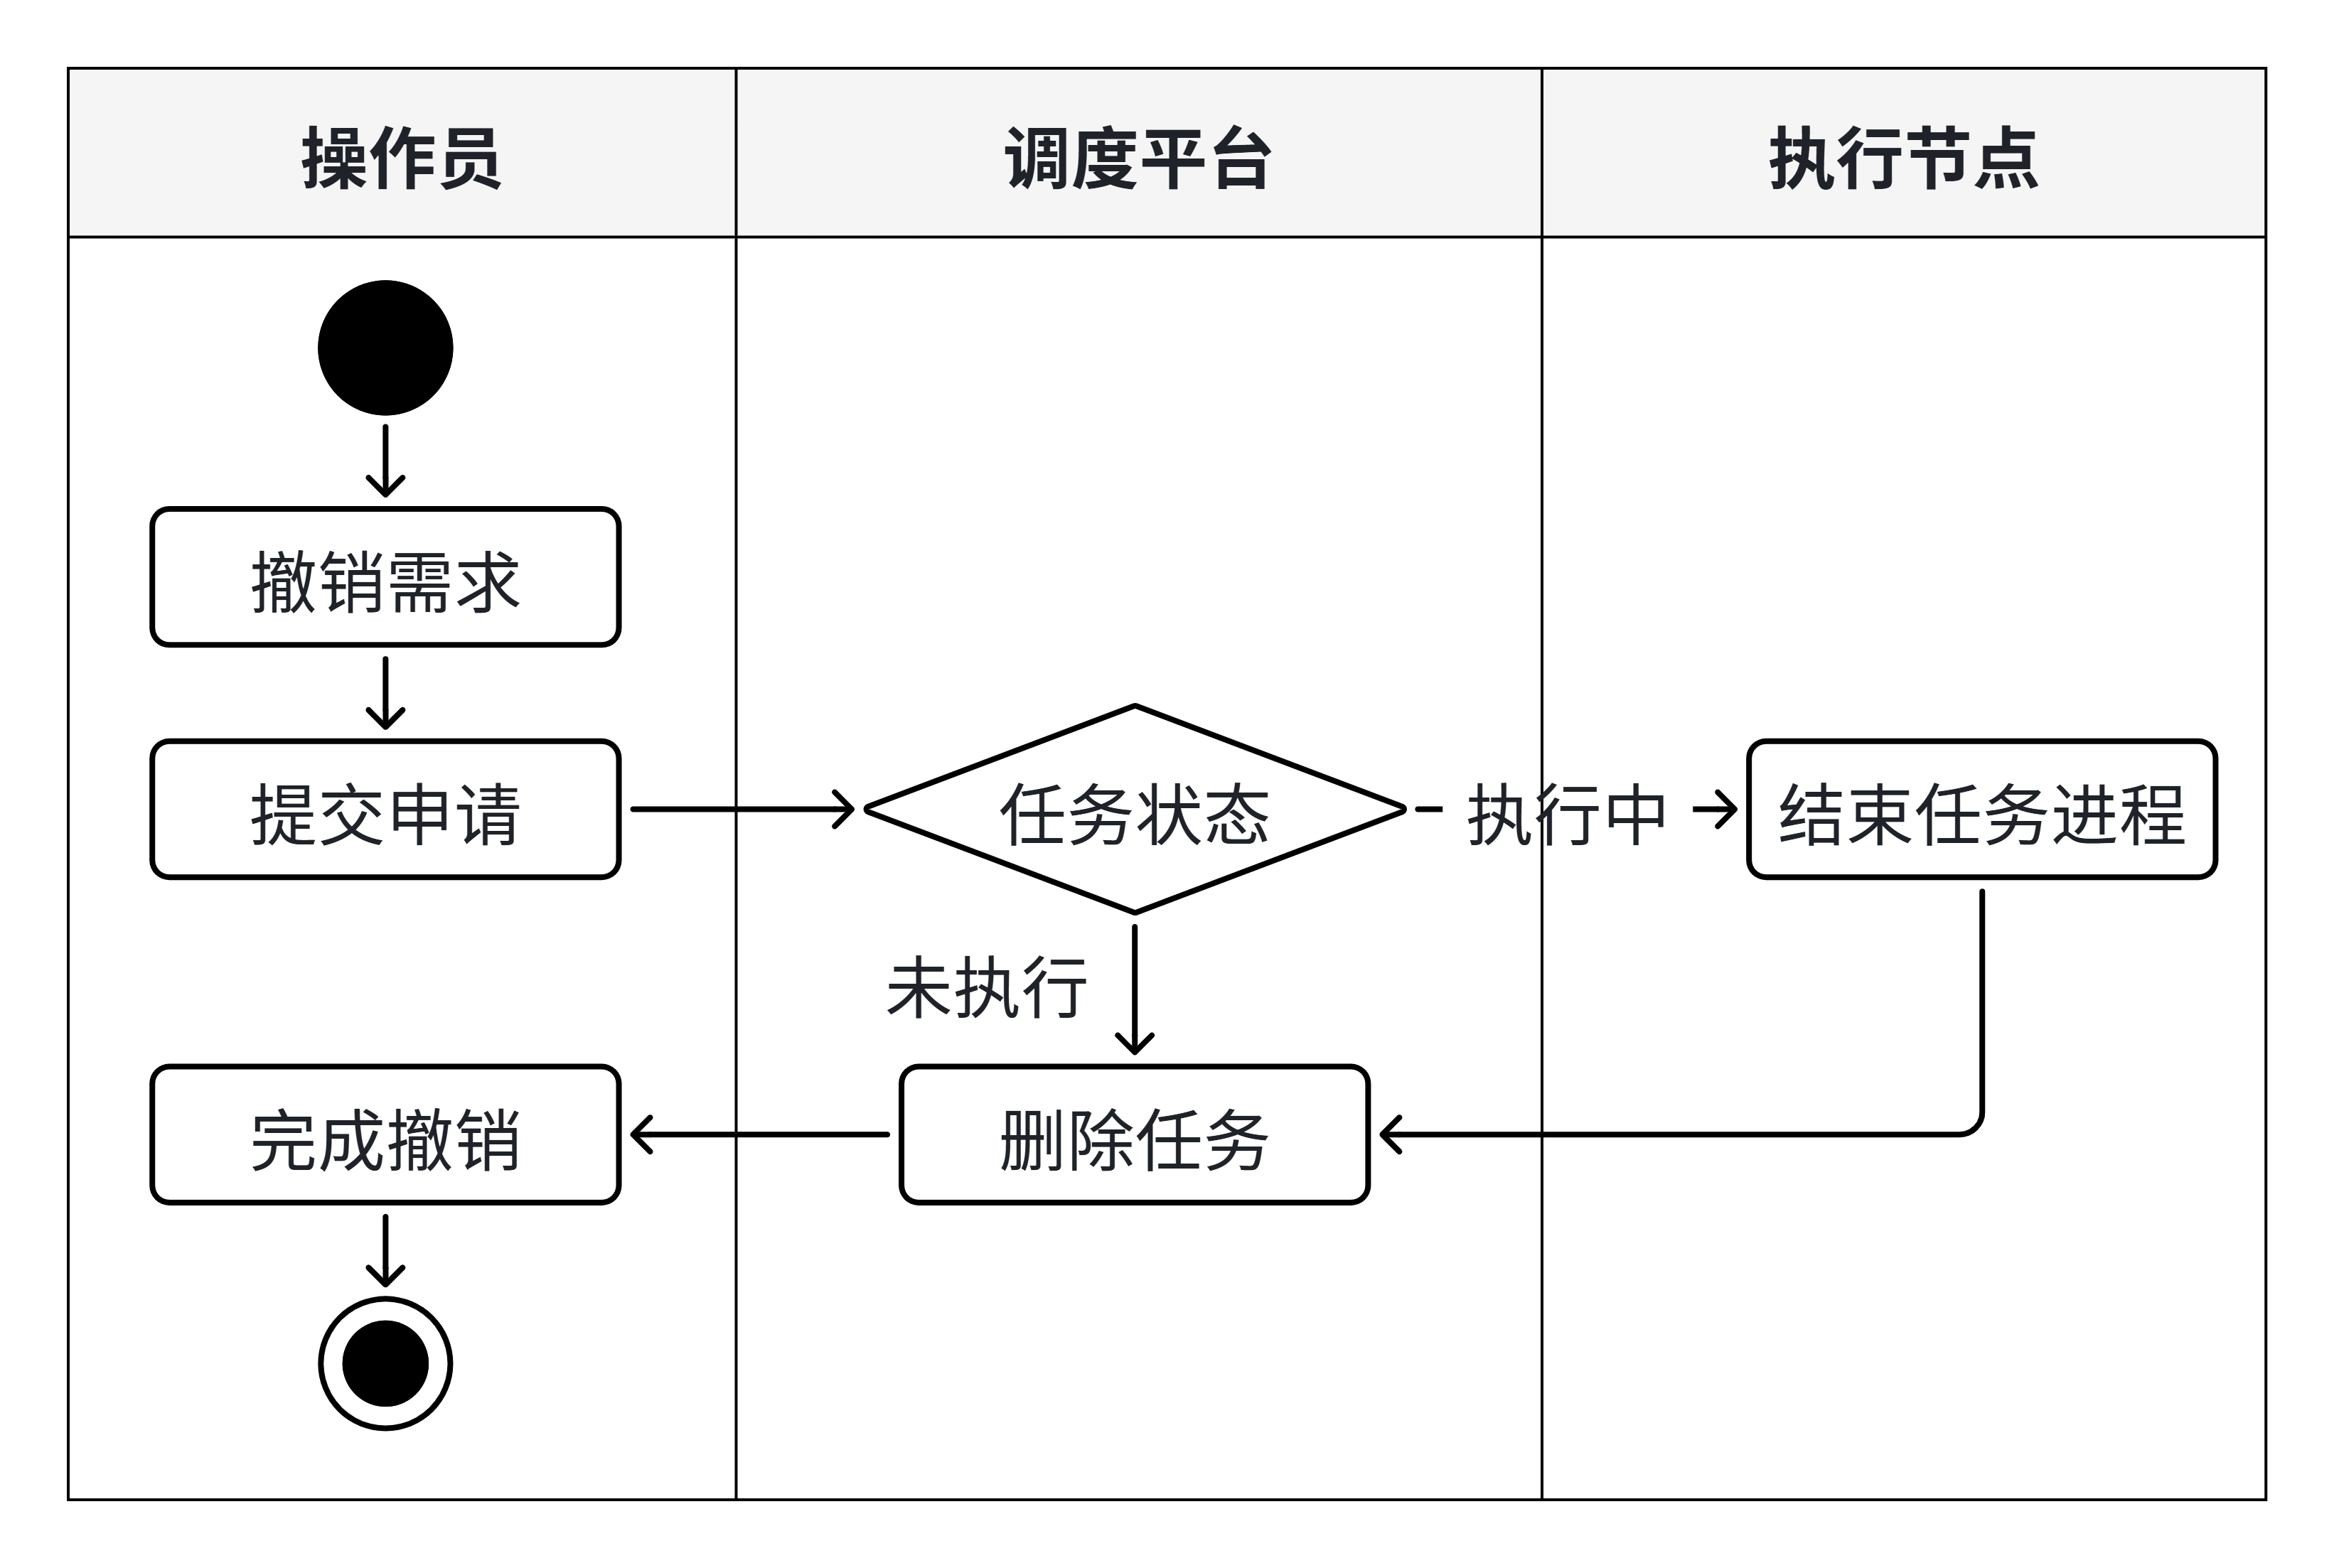
\includegraphics[width=0.9\linewidth]{figures/4/任务撤销流程.png}
    \caption{任务撤销泳道图}
    \label{fig:enter-label}
\end{figure}

\subsection{异常捕获机制}

本系统还需承接并处理任务执行过程中发生的异常情况。借助Python便捷的异常处理流程，本系统能够轻松识别任务运行时出现的错误。作为一种基于解释器的编程语言，它不会强制开发人员在开发过程中捕获异常\cite{s0218194022500814}，而AI任务的代码相对灵活，不安全的代码极有可能在没有经过全面的代码评审环节，就发布到平台上，因此极有可能在任务运行时抛出异常。本系统会捕获所有异常，并展开初步分析。倘若AI任务代码依照约定将具体异常日志打印到指定目录，本系统还能够整理这些日志，形成报表，并推送给操作员。异常发生后，所有中间文件和结果文件都会被上传，方便操作员自由下载，进而查看异常发生的原因。

\section{数据库表设计}

\subsection{数据库实体关系设计}

本系统核心数据模型由五个实体组成：用户、任务组、任务、附件以及资源占用记录。各实体的属性定义如下：

\begin{enumerate}
    \item 用户实体：存储身份及权限基础信息，包括用户ID、名称、账号有效性、注册时间及角色属性。
    \item 任务组实体：作为权限管理与资源隔离的基本单位，包含ID、名称、创建者、创建/更新/删除时间及删除状态位。
    \item 任务实体：记录AI调度的核心业务数据，包含ID、名称、创建者、生命周期时间戳（创建/修改/完成时间）、当前状态及异构参数列表。
    \item 附件实体：管理云端存储文件元数据，包含ID、显示名、对象存储URL、上传时间、上传者及删除标识。
    \item 资源占用记录实体：辅助调度算法进行互斥判断，包含记录ID、关联任务ID、资源名称及失效状态。
\end{enumerate}

\begin{figure}[htbp]
    \centering
    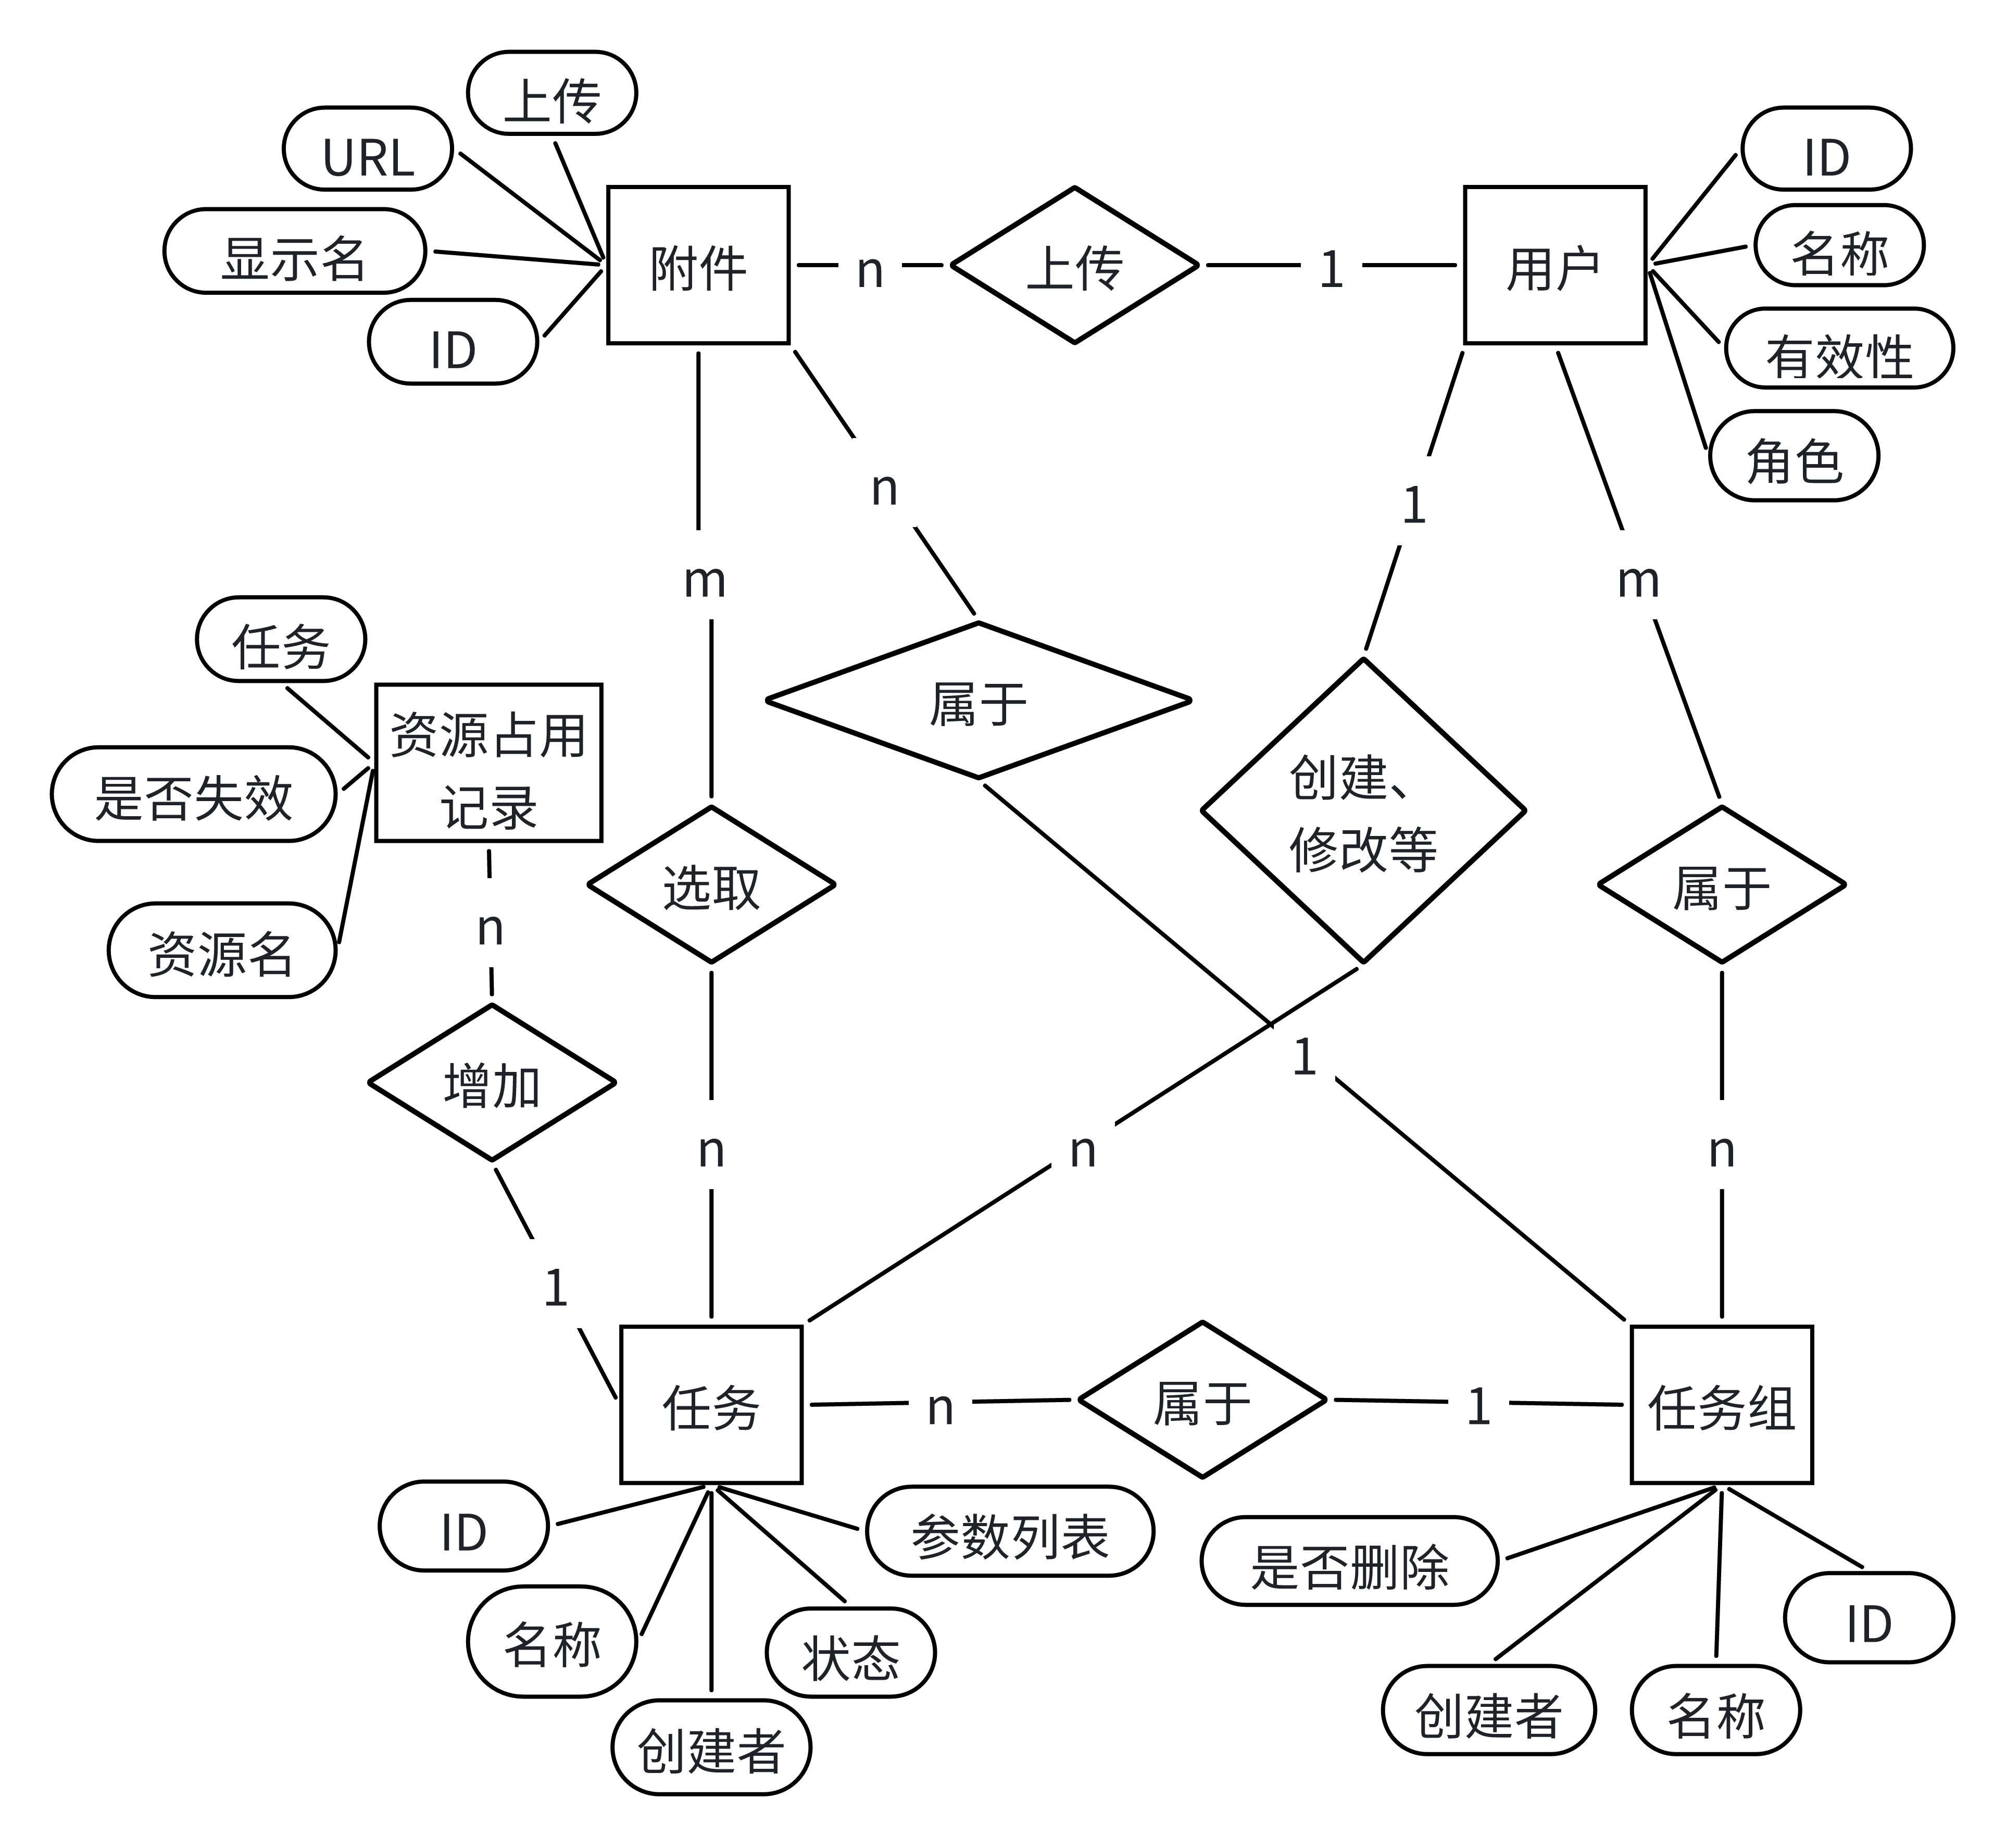
\includegraphics[width=\linewidth]{figures/4/数据库实体间关系.png}
    \caption{数据库实体间关系}
    \label{fig:enter-label}
\end{figure}

本系统的数据库实体关系如图4.9所示。

实体的相互关联逻辑梳理如下：

\begin{enumerate}
    \item 以“任务”为核心的关联逻辑。任务实体是系统逻辑的交汇点。用户与任务呈1:N关系，即一名用户可创建多个任务，但每个任务仅对应唯一创建者；任务组与任务呈1:N关系，确保任务在逻辑上归属于特定项目组以实现隔离。任务与附件呈M:N多对多关系，一个任务可选取多个预设附件，同一附件也可被不同任务重复引用。任务与资源占用记录呈1:N关系，用于精细化记录单个任务对多个临界资源的占用情况。
    \item 以“用户与权限”为核心的关联逻辑。用户是系统的操作主体。用户与任务组呈M:N关系，即用户可跨组协作，任务组也可包含多名成员，这种灵活的绑定关系支撑了系统的权限校验机制。此外，用户与附件呈1:N关系，明确了云文件的归属权。
    \item 以“隔离与调度”为核心的关联逻辑。任务组与附件呈1:N关系，实现了不同组间AI素材的逻辑隔离。资源占用记录主要服务于调度算法的互斥判断，通过与任务表的关联，协助调度器识别当前的算力冲突，保障多任务并发环境下的执行安全。
\end{enumerate}

本系统的类图如图4.10所示，该图将上述实体关系以类图的形式表达。

\begin{figure}[htbp]
    \centering
    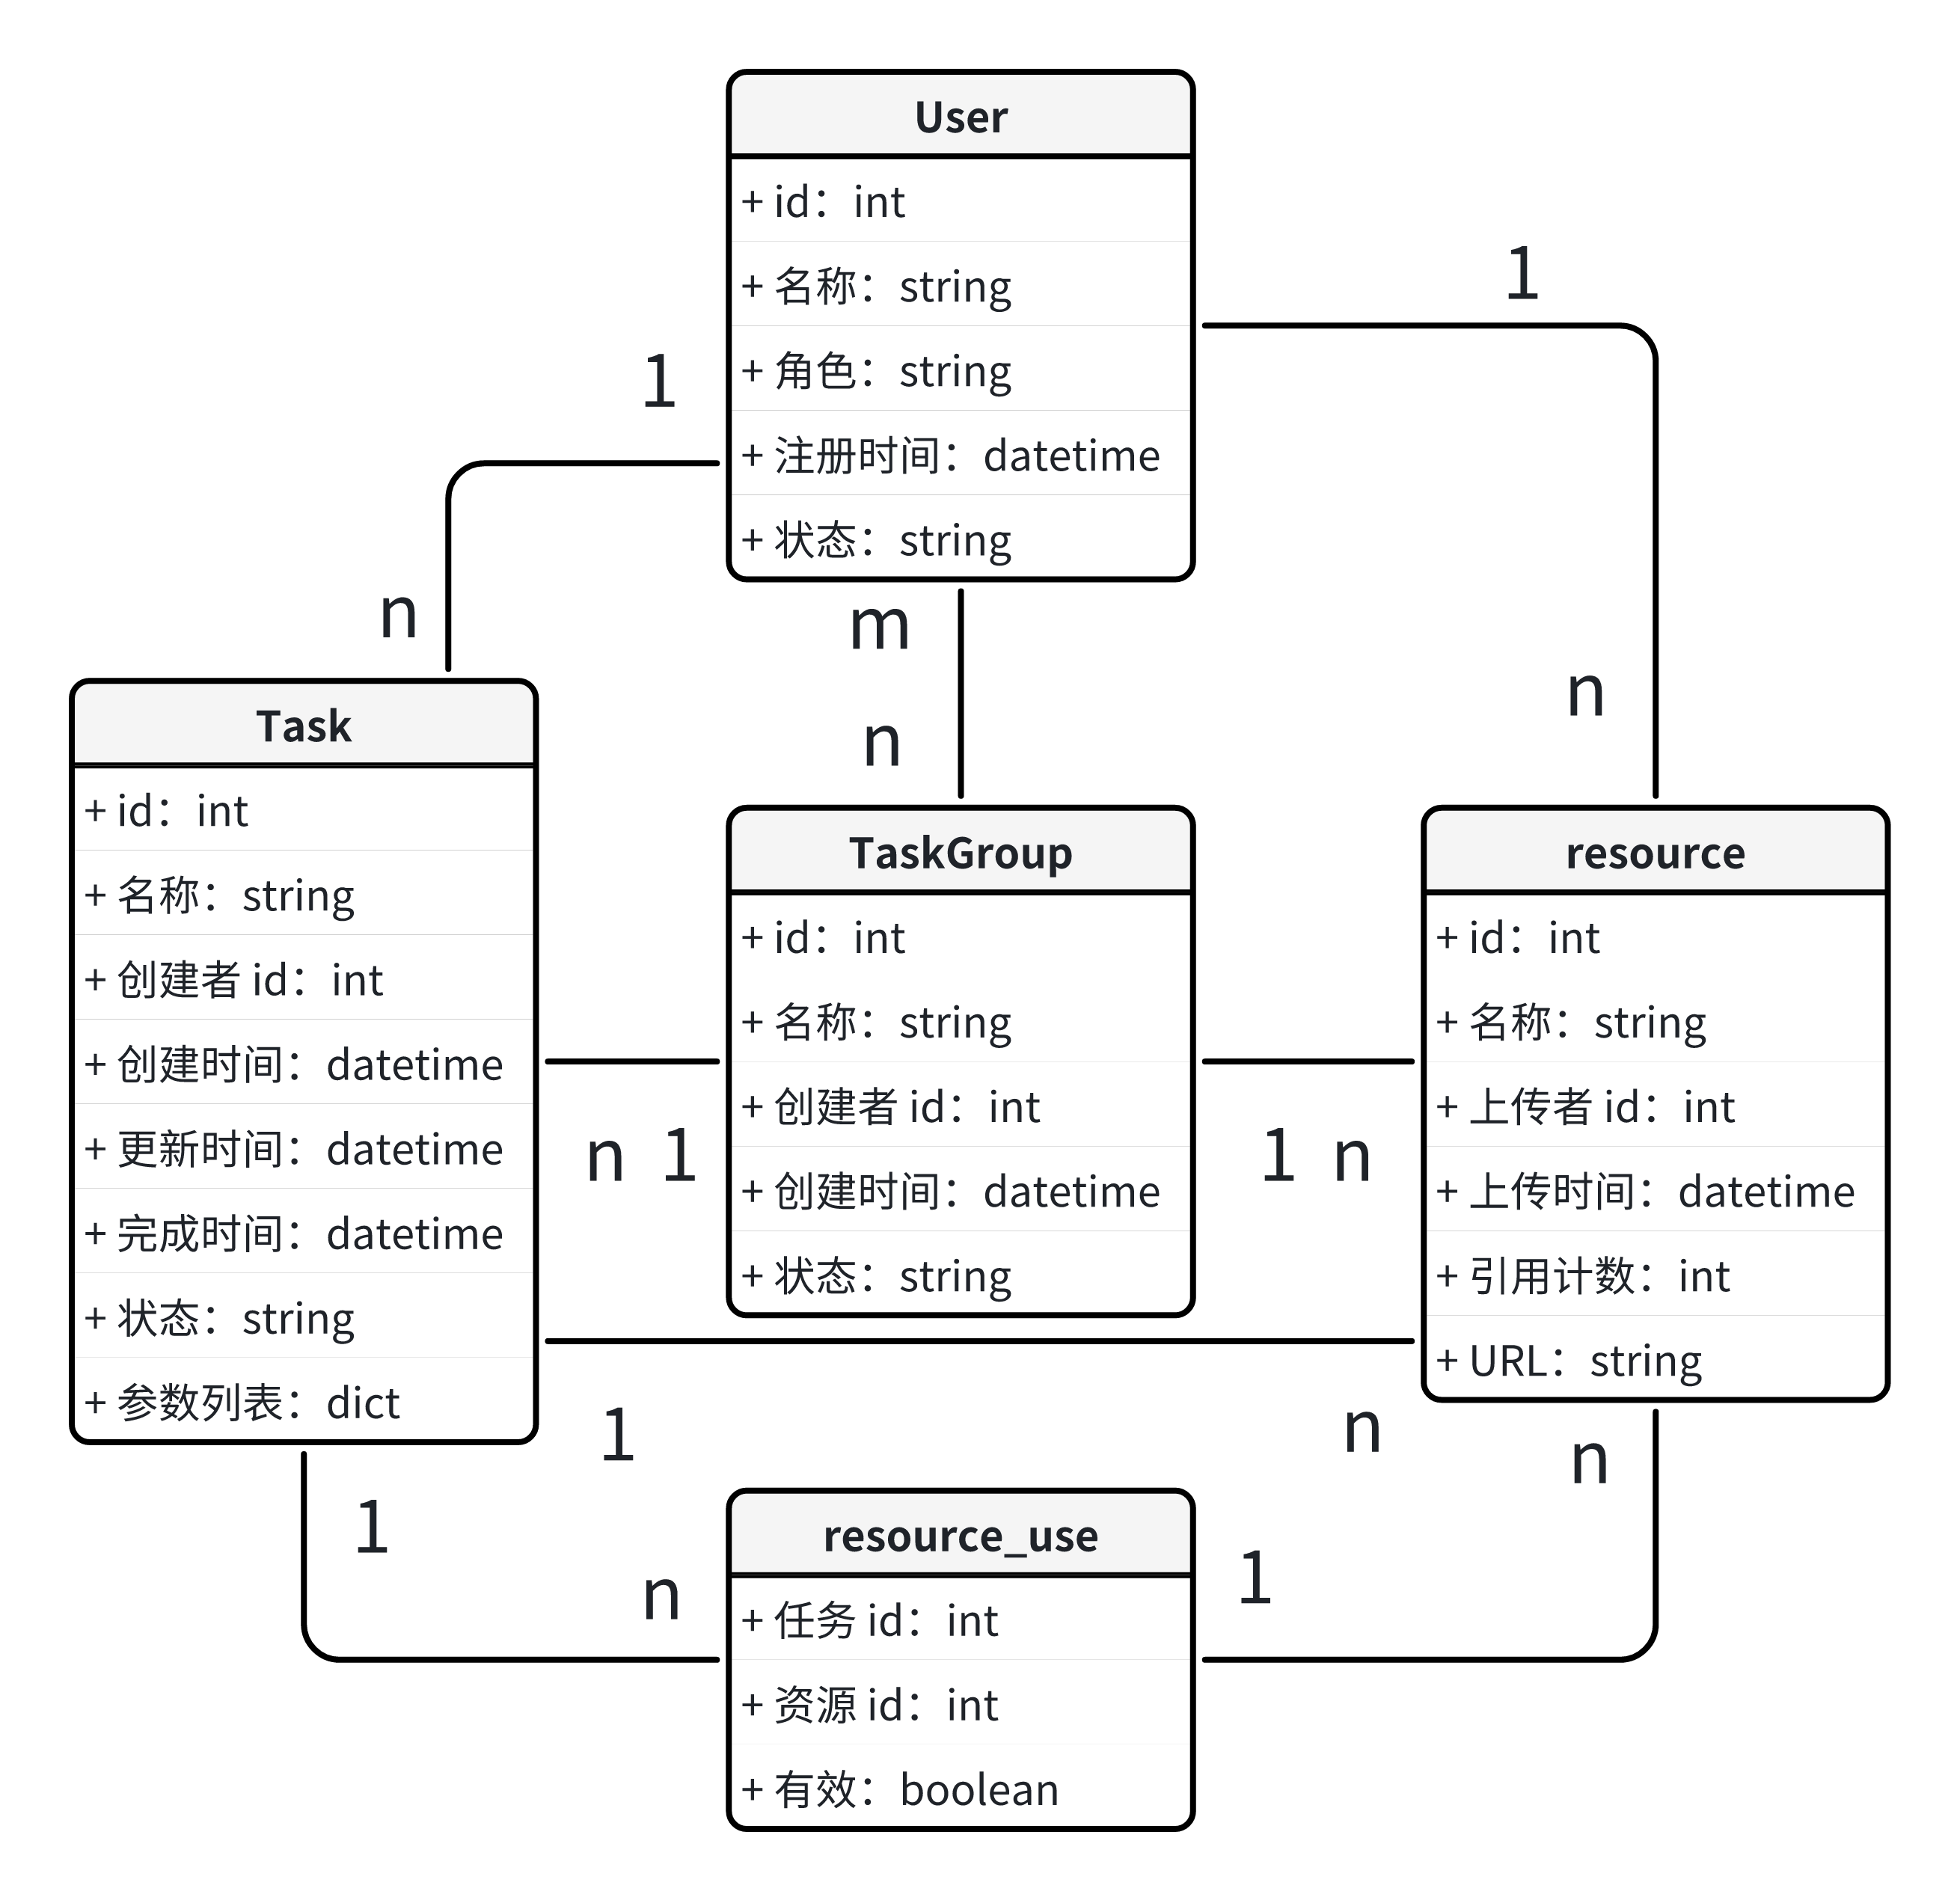
\includegraphics[width=\linewidth]{figures/4/本系统类图.png}
    \caption{本系统类图}
    \label{fig:enter-label}
\end{figure}

\subsection{数据库表设计}

本系统采用轻量级关系型数据库PostgreSQL进行数据持久化。根据实体功能及关联逻辑，将数据库表划分为基础权限类、核心业务类以及调度支撑类三个部分。

基础权限类表是构建整套调度系统安全底座的关键核心组件，在系统架构中主要承担着身份验证（Authentication）与访问控制（Access Control）的基础职能。该表的设计不仅能够严防非授权操作对高价值算力资源的非法侵占，更从技术维度确保了临界资源分配的审计合规性，为系统后续实现自动化准入决策与复杂的资源互斥分析提供了坚实且可信的操作上下文保障。

\begin{table}[htbp]
    \centering
    \caption{用户表}
    \begin{tabular}{llllll}
        \toprule
         序号 & 字段名 & 字段说明 & 类型 & 是否为空 & 说明 \\
         \midrule
            1 & id & 用户ID & int & N & PK\\
            2 & name & 用户名 & int & N & unique\\
            3 & valid & 账号是否有效 & boolean & N & \\
            4 & is\_delete & 是否已被删除 & boolean & N & \\
            5 & create\_time & 创建时间 & datetime & N & \\
            6 & update\_time & 资料更新时间 & datetime & N & \\
            7 & delete\_time & 删除时间 & datetime & N & \\
            8 & avatar & 头像链接 & varchar(200) & N & \\
         \bottomrule
    \end{tabular}
    \label{tab:my_label}
\end{table}

用户表如表4.1所示，该表用于存储操作员的核心属性及状态。在AI多任务调度流程中，系统需依托该表校验操作者的身份合法性，并为其分配相应的管理角色。表内设计的valid与is\_delete双重标识位，确保了在人员变动或账号注销时，系统能实现平滑的权限回收，保障安全。

\begin{table}[htbp]
    \centering
    \caption{任务组表}
    \begin{tabular}{llllll}
        \toprule
        序号 & 字段名 & 字段说明 & 类型 & 是否为空 & 说明 \\
        \midrule
1 & id & 任务组ID & int & N & PK \\
2 & name & 任务组名称 & int & N & unique \\
3 & owner & 任务组创建者 & varchar(200) & N &  \\
4 & is\_delete & 是否已被删除 & boolean & N &  \\
5 & create\_time & 创建时间 & datetime & N &  \\
6 & update\_time & 更新时间 & datetime & N &  \\
7 & delete\_time & 删除时间 & datetime & N &  \\
        \bottomrule
    \end{tabular}
    \label{tab:my_label}
\end{table}

任务组表如表4.2所示，该表是实现多租户隔离与资源归属管理的核心工具。针对大模型研发中不同业务团队共用底层集群的现状，任务组通过逻辑划分界定了任务与附件的所属权边界。这种设计不仅能有效规避跨组误操作引发的生产事故，还为后续针对特定业务线进行算力配额统计与审计提供了关键的元数据支撑。

核心业务类表作为系统架构中的逻辑基石，是支撑AI大模型异构数据深度适配、任务全生命周期精细化追踪以及复杂计算结果高可靠持久化的核心数据载体。针对当前主流调度方案在应对人工智能大模型任务时暴露出的适配性匮乏、非结构化参数校验门槛过高以及数据描述维度过于僵化等行业痛点，本系统立足于现代软件工程建模思想，在底层数据结构设计上实施了深度的范式优化。通过引入面向AI特性的Schema-less多维数据存储模型，并构建基于动态参数画像的关联机制，系统不仅能够敏锐感知并无缝兼容Prompt模板、采样超参数等高维度异构输入，更通过建立严密的任务状态机映射体系，实现了对调度指令从初始注入、排队挂起到最终结果回收的全流程数据闭环，从而为攻克AI多任务场景下的适配难题与调度瓶颈提供了稳固的数字化底座。

\begin{table}[htbp]
    \centering
    \caption{任务表}
    \begin{tabular}{llllll}
        \toprule
序号 & 字段名 & 字段说明 & 类型 & 是否为空 & 说明 \\
        \midrule
1 & id & 任务ID & int & N & PK \\
2 & name & 任务名称 & int & N & unique \\
3 & owner & 任务创建者 & varchar(200) & N &  \\
4 & kind & 任务类型 & varchar(200) & N &  \\
5 & is\_delete & 是否已被删除 & boolean & N &  \\
6 & update\_time & 更新时间 & dateTime & N &  \\
7 & datafiles & 数据文件列表 & varchar(1000) & Y &  \\
8 & queue\_task\_id & 在任务队列中的id & varchar(200) & Y &  \\
9 & progress & 任务进度 & JSON & Y &  \\
10 & result & 任务结果 & JSON & Y &  \\
11 & params & 任务启动参数 & JSON & Y &  \\
        \bottomrule
    \end{tabular}
    \label{tab:my_label}
\end{table}

任务表如表4.3所示，该表是调度指令的核心。为应对AI大模型任务中Prompt模板、采样参数以及模型超参数的异构性，系统采用JSON格式设计了params字段。这种Schema-less的设计能够灵活存储大模型任务的异构参数画像，有效解决了传统结构化表难以适配多样化AI任务的问题。此外，queue\_task\_id实现了业务逻辑层与底层Celery分布式队列的解耦关联，与之配套的 progress 与 result 字段采用JSON 类型，旨在构建一套完整的任务全生命周期观测体系。其中，progress 字段不局限于记录单一的百分比进度，更支持动态存储中间推理步骤、分段耗时等时序快照；而 result 字段则负责封装复杂的推理产出，包括但不限于文本响应、分词权重或多模态元数据。

\begin{table}[htbp]
    \centering
    \caption{附件表}
    \begin{tabular}{llllll}
        \toprule
        序号 & 字段名 & 字段说明 & 类型 & 是否为空 & 说明 \\
        \midrule
1 & id & 附件ID & int & N & PK \\
2 & name & 附件名称 & int & N & unique \\
3 & owner & 附件创建者 & varchar(200) & N &  \\
4 & is\_delete & 是否已被删除 & boolean & N &  \\
5 & update\_time & 更新时间 & dateTime & N &  \\
6 & url & 下载链接 & varchar(200) & N &  \\
7 & status & 数据集状态 & int & N &  \\
8 & count & 数据集大小 & int & N &  \\
9 & ref & 引用数 & int & N &  \\
        \bottomrule
    \end{tabular}
    \label{tab:my_label}
\end{table}

附件表如表4.4所示，该表专门用于管理大模型任务涉及的海量训练素材、验证数据集以及模型权重文件。由于AI任务具备强数据依赖的特征，附件表通过url字段对接公司对象存储服务，并利用status与count字段实现对异构素材的即时索引与量化评估。值得注意的是，表中设计的引用计数机制（ref）能够实时监测附件被不同任务调用的频率，为系统后续的存储空间自动回收与冗余清理提供了决策依据，从而在保障数据快速拉取的同时，最大化存储资源的利用率。

调度支撑类表是实现针对GPU等稀缺算力资源进行互斥识别与并发优化的关键数据底座。由于AI大模型任务在执行过程中对底层硬件具有显著的强排他性特征，若调度层缺乏对资源状态的实时感知能力，往往只能采取保守的串行策略，从而造成严重的算力资源浪费。

\begin{table}[htbp]
    \centering
    \caption{资源占用表}
    \begin{tabular}{llllll}
        \toprule
        序号 & 字段名 & 字段说明 & 类型 & 是否为空 & 说明 \\
        \midrule
1 & id & 记录ID & int & N & PK \\
2 & task\_id & 任务ID & int & N &  \\
3 & resource\_name & 资源名称 & varchar(200) & N &  \\
4 & is\_delete & 记录是否已被删除 & boolean & N &  \\
5 & create\_time & 占用记录创建时间 & datetime & N &  \\
6 & delete\_time & 删除时间 & dateTime & N &  \\
        \bottomrule
    \end{tabular}
    \label{tab:my_label}
\end{table}

资源占用表如表4.5所示，该表在系统中充当了全局“算力锁中心”的职能。通过动态记录task\_id与具体resource\_name（如特定的GPU编号或显存单元）的映射关系，系统能够以细粒度的方式实时追踪各临界资源的独占状态。在调度决策阶段，调度引擎通过检索该表执行资源互斥智能分析算法：若目标资源处于锁定状态且记录有效，则任务进入挂起队列；若资源空闲，则即时写入占用记录。表中的is\_delete与delete\_time字段配合执行层的异常捕获机制，实现了算力资源的即时释放与状态回收回滚。这一设计从底层数据结构上打破了调度流程的“黑盒”状态，为实现由传统串行执行向高效并发调度的转型提供了核心决策依据。

\section{本章小结}

本章初步介绍了系统的模块、子模块，以及数据库关系和表结构。在第一小节里，阐述了本系统的设计原则。基于上一章提出的几个方向性需求，此部分做出原则性规划，为系统设计明确总体方向与准则；第二小节对本系统的整体结构展开介绍，使读者初步认识系统的几大模块，构建起对系统架构的宏观印象；第三小节聚焦网络接入层，简要介绍了该层的权限鉴定和数据校验功能，这两个功能是保障网络接入安全与数据准确性的关键；第四小节介绍任务调度层。一方面对任务、资源可用性检测的自研算法予以说明，展现系统在任务与资源管理方面的独特方法，另一方面介绍负载均衡、数据同步、容错与恢复机制，这些机制确保任务调度的高效与稳定；第五小节谈及相对简单的任务执行层，主要介绍了附件和参数的初步处理、任务撤销与编辑，以及任务异常捕获机制，它们是任务顺利执行的重要保障；第六小节讲解本系统的数据库设计，主要涉及数据库实体关系和数据库表结构，这是系统数据存储与管理的基础。

\makeatletter
\@openrightfalse
\makeatother
\chapter{详细设计与实现}

本章将详细拆解系统的具体实现过程，核心逻辑是将工程落地与前期的研究方向深度绑定。针对AI任务配性差的痛点，本工作在API接入层与执行层建立了参数画像与自动纠偏机制，把繁琐的人工纠错转化成了系统的自动化本能；为了解决调度决策太依赖人工的问题，调度层引入了环境感知的自动决策引擎；而针对GPU等贵重资源出现占用冲突所引发的效率瓶颈，本系统通过互斥分析算法实现了从低效串行到高效并发的质变。这些技术实现不仅让系统能看懂AI任务，更从底层保障了多任务场景下的算力利用率与运行稳健性。

\section{API接入层详细设计}

API接入层作为系统的首要入口，承担着用户指令进入调度中枢的唯一通道角色。该层通过整合Docker容器化环境、服务治理组件及FastAPI异步框架，构建了稳固的运行基础设施，其设计核心聚焦于安全性与鲁棒性，分别由权限鉴定与数据校验两大模块负责，确保所有AI调度指令具备合法性与可靠性。

在研究方向的关联上，该层是解决AI适配性欠佳的关键环节。针对AI大模型任务参数复杂、人工录入易出错的痛点，本文利用数据校验模块建立了严密的参数画像与自动化纠偏逻辑，将以往因类型不符或格式错误所引发的系统崩溃问题，在接入端通过技术手段予以消除，显著提升了系统对异构AI数据的处理能力。同时，严密的权限鉴定机制确保了仅授权任务可调用昂贵的GPU算力，为后续调度层在纯净、安全的数据环境下解决“自动化决策”与“资源互斥分析”问题奠定了坚实基础。

\subsection{权限鉴定模块}

安全性在本系统中不仅是基础的准入要求，更是支撑AI多任务调度的前置屏障。在AI大模型研发场景下，GPU等算力资源不仅稀缺，且租赁成本极高，任何未经授权的调用或非法的任务下发，都将直接导致昂贵计算资源的无效空耗。尽管系统部署于公司内网，但在数万员工协同工作的大型环境下，内网身份并不等同于操作可信。因此，引入严格的身份认证机制，是防范资源误用的首要措施。

针对本文所研究的多任务场景，本工作引入了“任务组”隔离机制：通过对用户角色与任务组进行M:N的关系映射，确保操作员只能在被授权的业务范围内创建、修改或撤销任务。该设计深度契合研究背景中对“资源浪费”的治理需求，通过权限锁定，从源头上杜绝因跨团队误操作而引发的任务冲突或算力抢占。这不仅保障了数据的私密性，也为后续调度层执行“资源互斥分析”提供了纯净且可控的初始状态，从而确保系统在复杂环境下依然能够维持高度的稳定性。其主要流程如图5.1所示。

\begin{figure}[htbp]
    \centering
    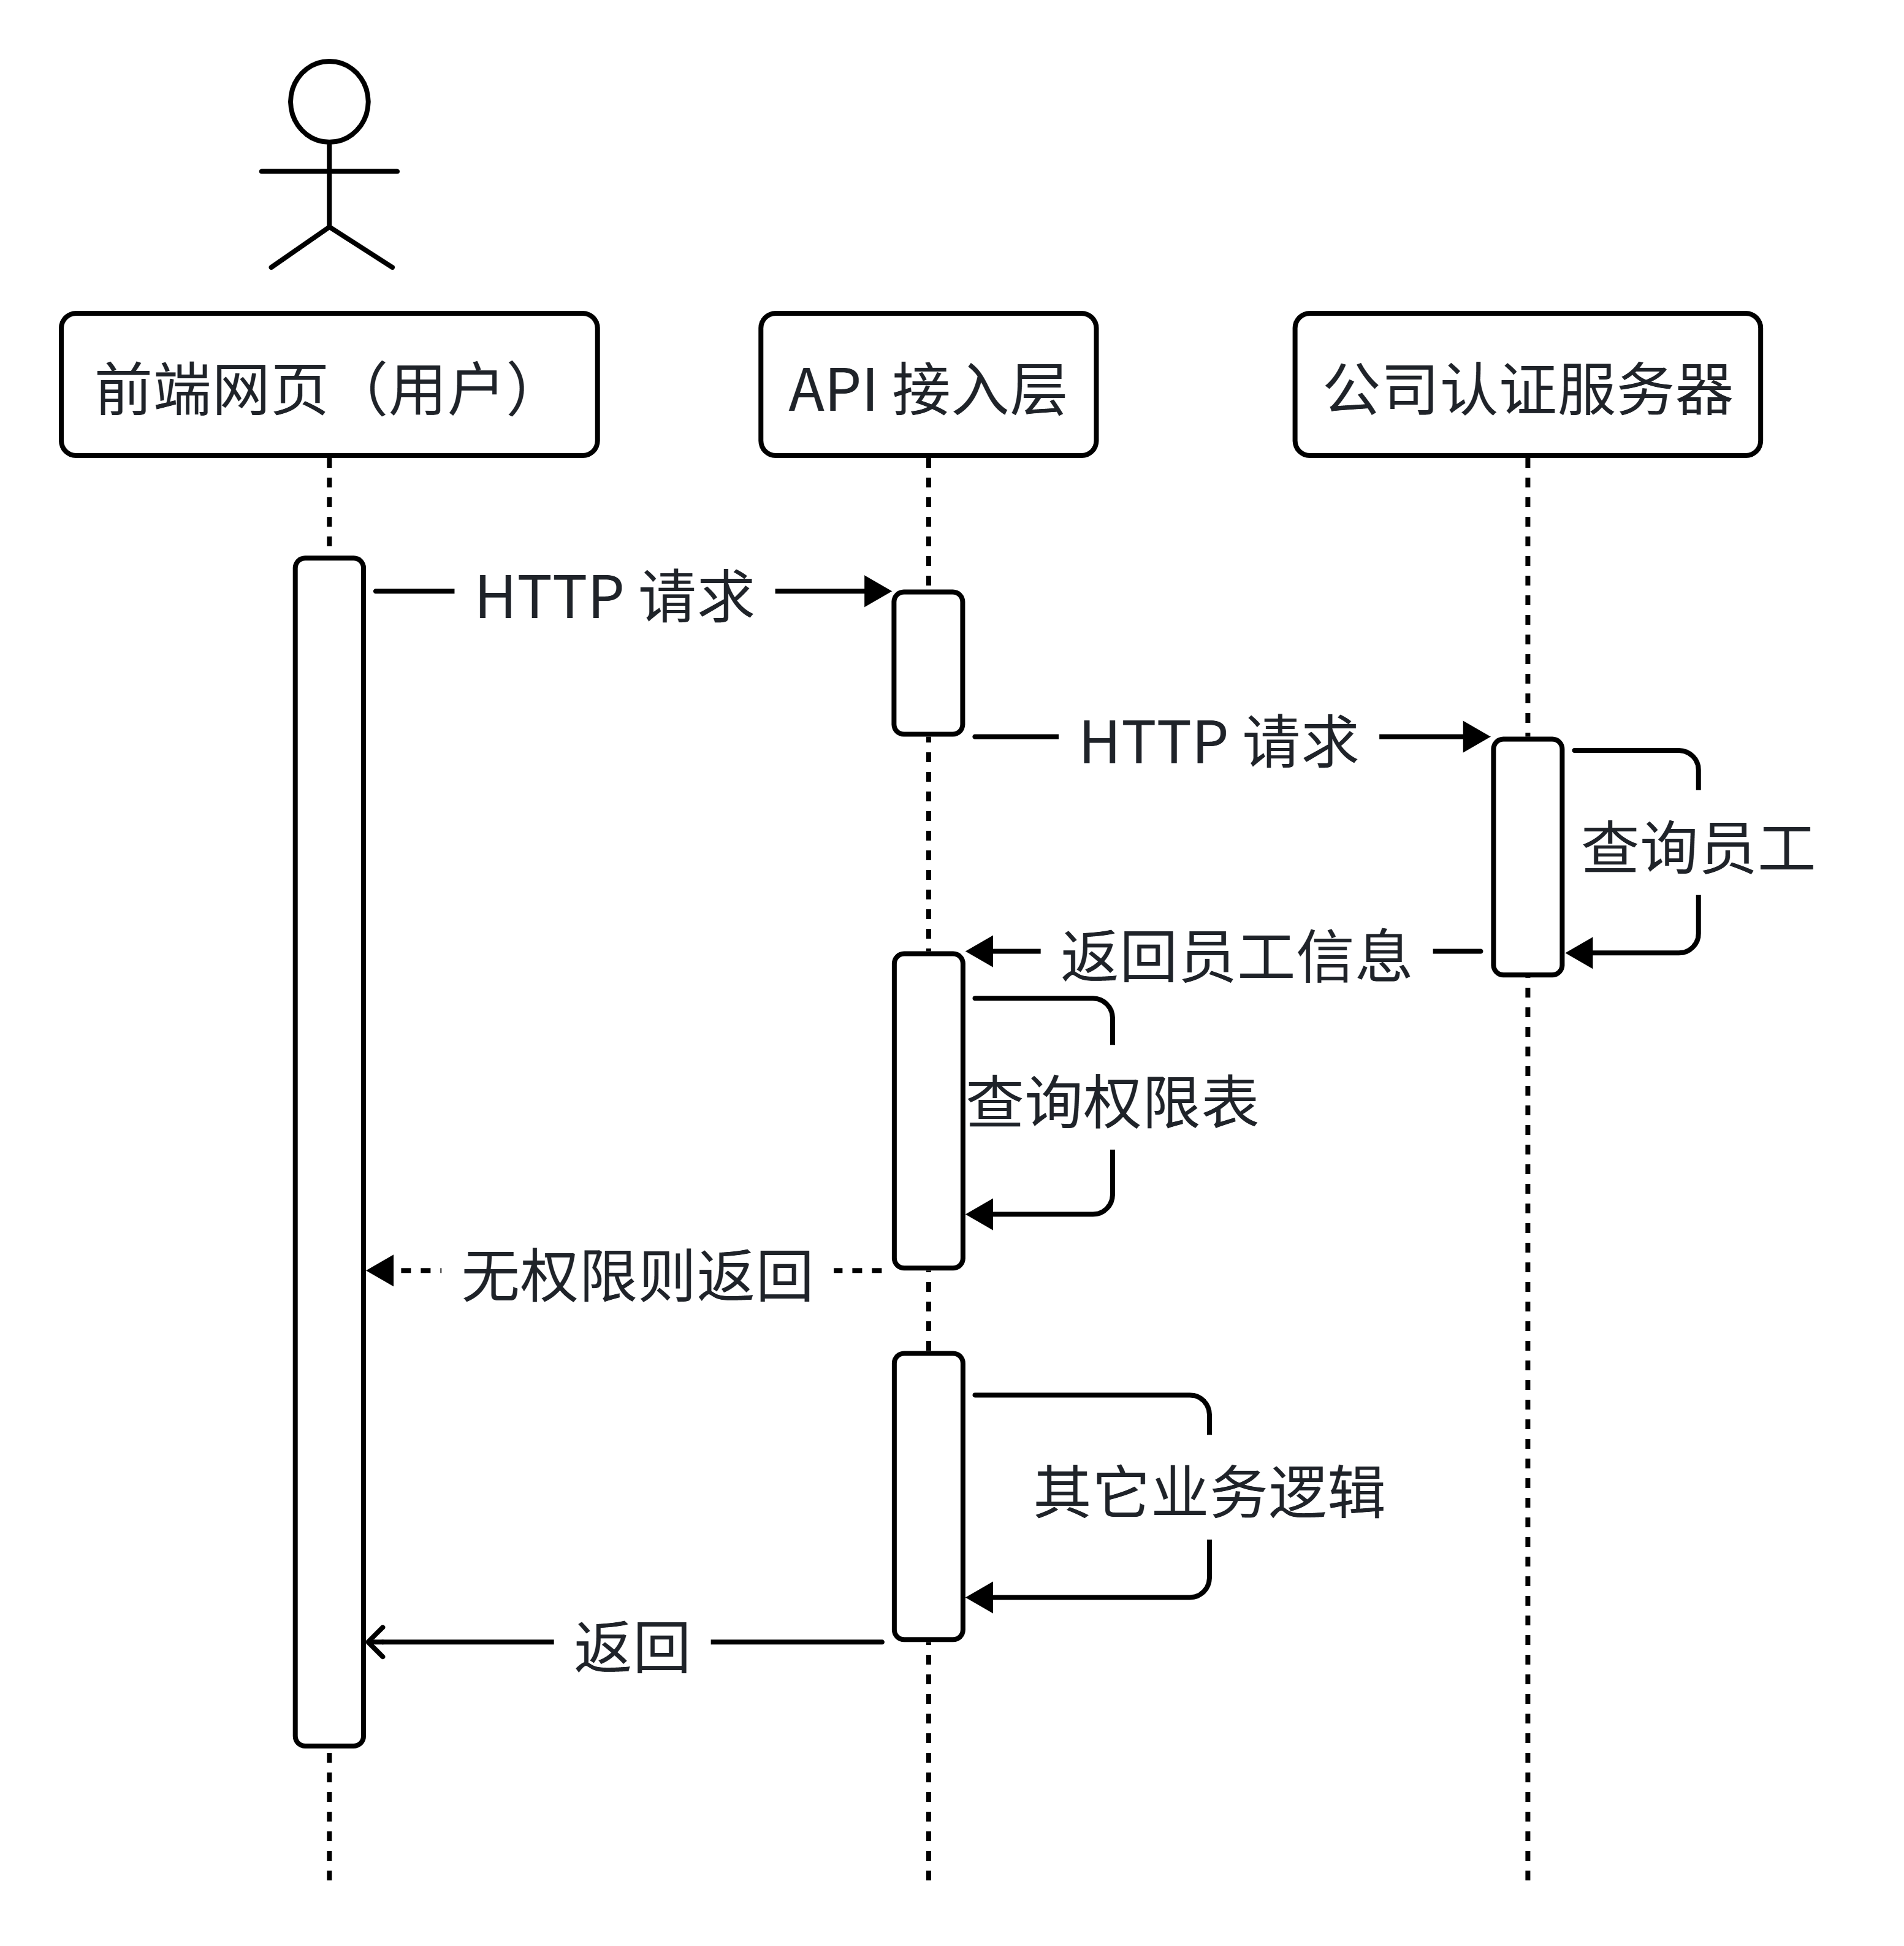
\includegraphics[width=0.8\linewidth]{figures/5/权限鉴定流程.png}
    \caption{权限鉴定时序图}
    \label{fig:enter-label}
\end{figure}

用户通过前端网页发起HTTP请求，该请求被发送至API接入层。随即，API接入层向公司认证服务器转发此HTTP请求。公司认证服务器接收请求后，查询员工相关信息，并将查询到的员工信息反馈给API接入层。而后，API接入层查询权限表。若查询结果显示用户无权限，便直接向前端网页返回无权限的结果；若确认用户有权限，API接入层则执行其他业务逻辑。待业务逻辑处理完毕，API接入层将最终结果返回给前端网页，至此完成一次从用户请求到系统反馈的完整交互流程。这一流程主要实现对用户操作的身份与权限校验，以此保障系统功能访问的安全性。

本系统在向公司认证服务器发出请求时，会携带用户提交的Cookie数据。公司认证服务器通过在浏览器Cookie中维护一个SessionID来管理用户会话。它拥有独立的超时过期策略，能够确保在一段时间未活动后，自动使会话失效，以此降低潜在风险。同时，公司认证服务器采用OAuth2.0机制，该机制通过授权流程，在不直接传递用户登录凭证的情况下，实现安全的第三方登录与信息交互，进一步保障登录信息安全。这些机制相互配合，为用户登录构建了严密的安全防线，有力保证了用户登录的安全性。

权限表存于本系统数据库，其主要功能是记录用户与任务组的所属关系。在此关系模式下，一个用户可操作多个任务组，一个任务组也能对应多个用户，呈现出m:n的多对多关系。当请求通过前文提及的身份认证环节后，便进入权限鉴定阶段。因公司管理策略规定用户名在全公司唯一且不可更改，本系统会依据用户名和任务组ID，查询相符的权限记录。若查询到记录，表明该请求满足鉴权要求，系统予以放行。另外，部分请求不涉及任务组相关概念，对于此类请求，本系统实行豁免政策，无需进行鉴权。

\subsection{数据校验模块}

在本系统中，鲁棒性具体表现为具备较高的交互容错性。当用户提交参数时，即使出现一些拼写错误，这些错误也会在API层被准确识别出来。系统能够自动对这些错误进行纠正，如此一来，既减少了用户重复操作的次数，又切实提升了用户的工作效率。本系统会对以下几种常见的输入错误进行自动修正：
\begin{enumerate}
	\item 全角标点：在输入数据过程中，因操作员未切换输入法，可能会输入全角的逗号或顿号。当系统处理此类数据时，像以逗号分隔数据形成列表这样的操作，就容易引发异常。为避免这种情况，本系统会先将这些全角符号自动转化为半角符号，然后再进行后续的数据处理工作。
	\item 多余的符号：当操作员输入列表或键值对类型的数据时，常常会直接从其他地方复制粘贴到本系统中。这种情况下，列表类型的参数前后可能会带有方括号，键值对类型的参数前后则可能带有花括号。针对此类情况，本系统在处理这些参数时，会自动检查参数前后是否存在多余符号，并将这些多余的方括号或花括号去除，以便后续更准确地处理数据。
	\item 数据类型错误：当系统要求输入的数据类型为整数（int）时，操作员可能由于疏忽，忘记数据类型要求而填入浮点数（float），这往往会致使后续的数据处理出现异常。对此，本系统具备智能的数据修正机制。在不改变数据值的前提下，系统会自动尝试将输入的浮点数修正为整数。例如，对于浮点数“3.0”，系统可将其修正为整数“3”。然而，如果修正操作会改变数据值，比如“3.5”，系统将不会应用此修正。而是以数据异常的形式及时通知操作员，告知其输入的数据类型与要求不符，以便操作员进行正确修改。
	\item 参数缺失：在系统运行过程中，有时会遇到版本更新的情况。若旧版本的界面操作请求被发送至新版本的服务程序，可能引发部分参数缺失的问题。针对这一状况，本系统借助Python生态中的pydantic库，对请求数据实施自动校验。一旦检测到请求数据未通过校验，系统便会返回相应的异常代码，以此提示出现异常，便于相关人员及时处理。
\end{enumerate}

数据校验模块的流程如图5.2所示。

\begin{figure}[htbp]
    \centering
    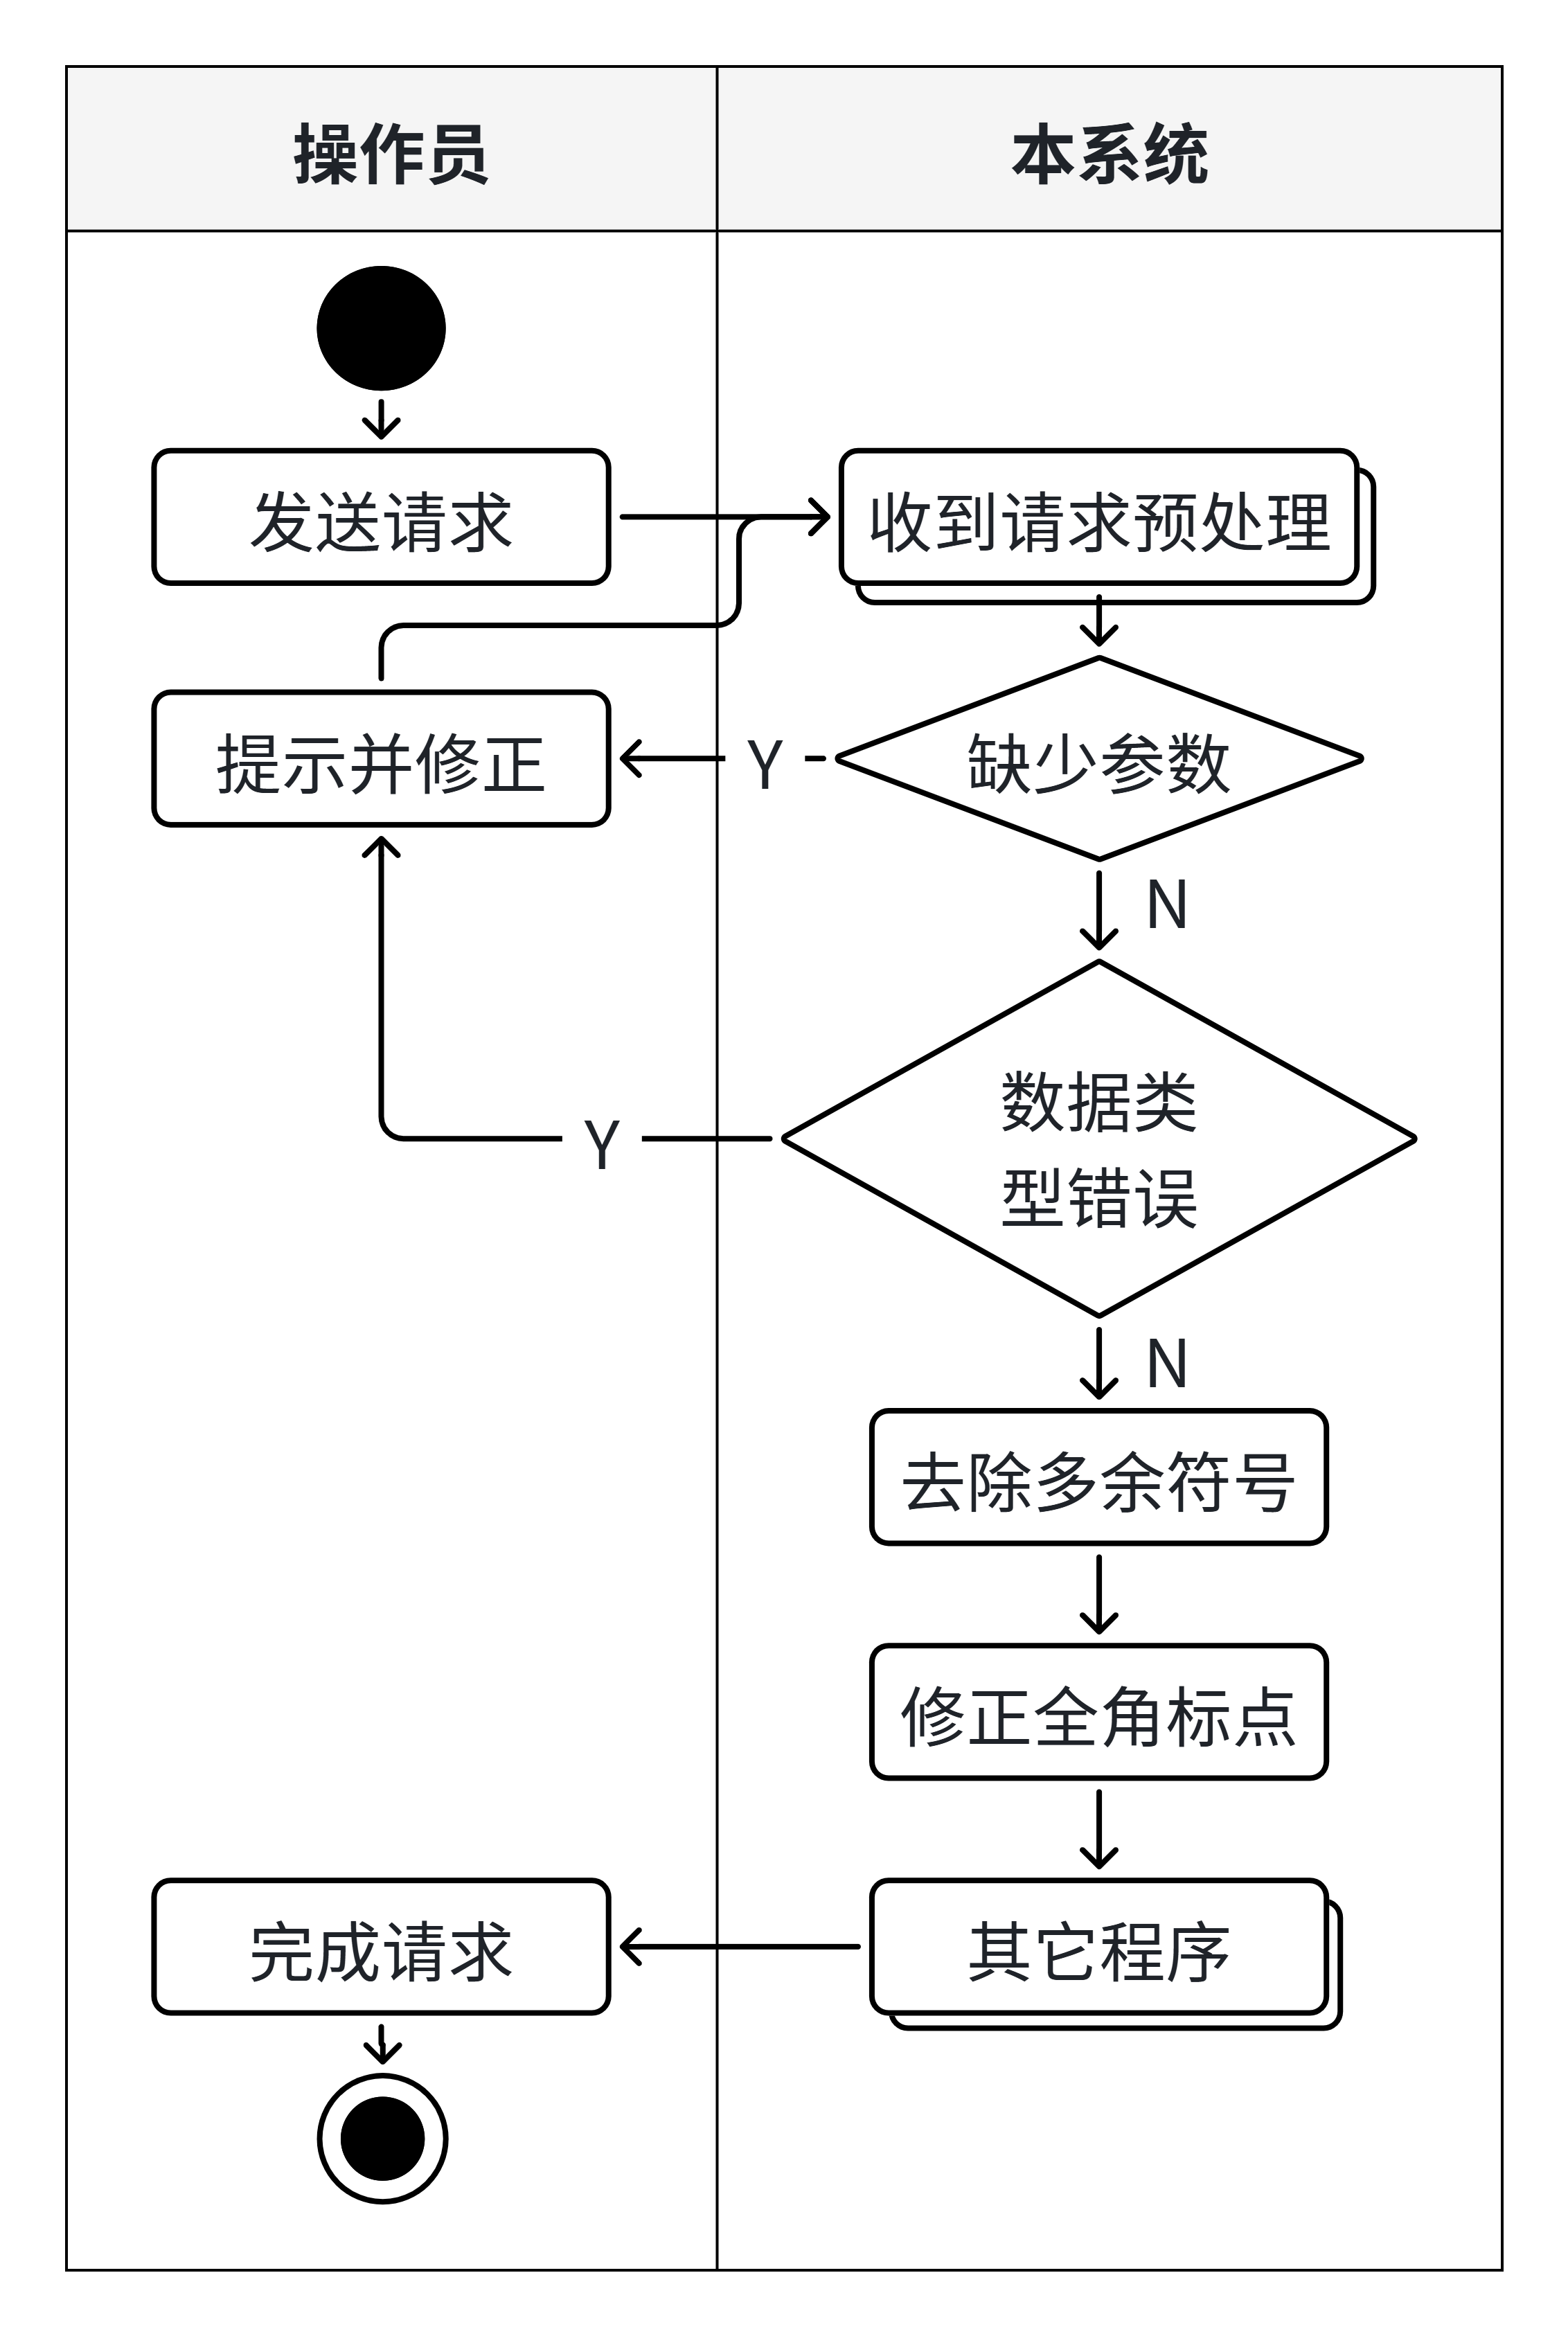
\includegraphics[width=0.8\linewidth]{figures/5/数据校验模块流程.png}
    \caption{数据校验模块泳道图}
    \label{fig:enter-label}
\end{figure}

\section{任务调度层详细设计}

本节着重介绍任务从API层提交至执行层执行前的相关过程。API层的设计较为简洁，其核心关注点在于权限验证以及数据的正确性，并不涉及对深层次需求与逻辑的处理。

当API层接收到任务后，会将任务简要地写入数据库，并将任务状态设为 “待调度”，同时把该任务添加至任务池。本系统前端网页操作员编辑任务到该任务被调度，整体的流程如图5.3所示。

\begin{figure}[htbp]
    \centering
    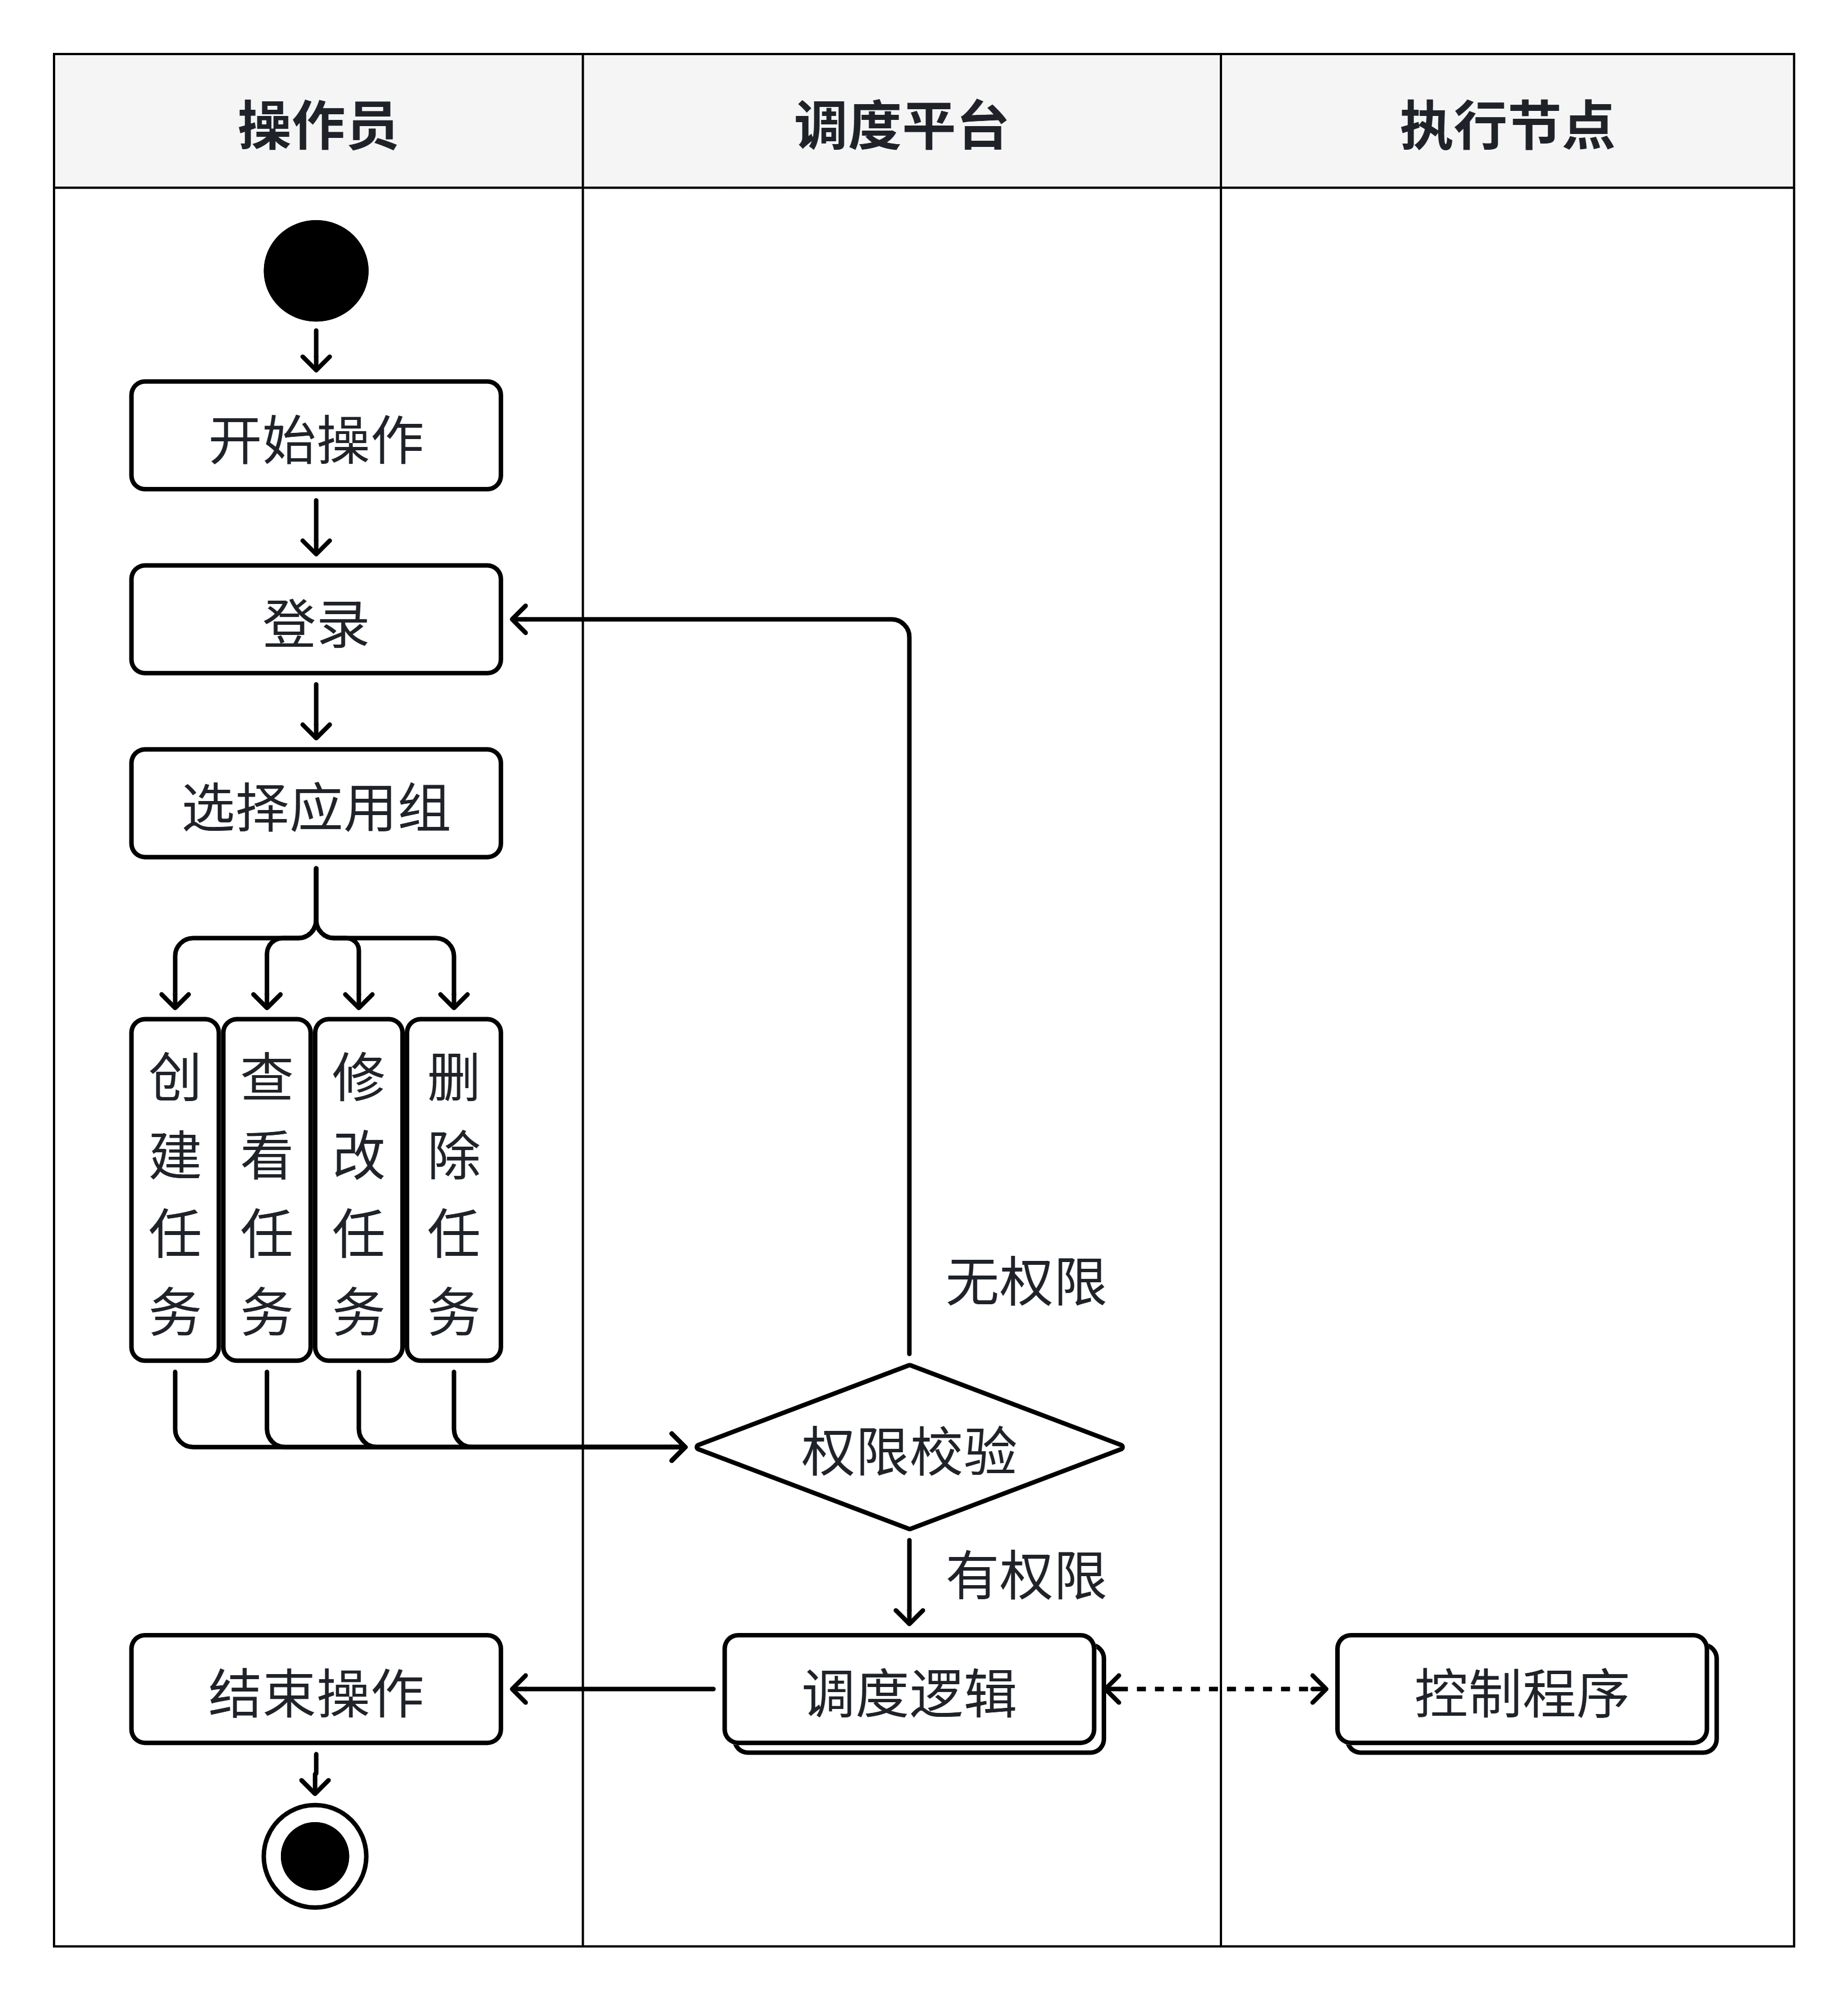
\includegraphics[width=\linewidth]{figures/5/任务操作流程图.png}
    \caption{任务操作泳道图}
    \label{fig:enter-label}
\end{figure}

本系统构建了一套任务状态管理模型，旨在实现对任务全生命周期的精细化追踪与实时监控。
该状态机不仅是调度系统的逻辑枢纽，为各模块间的协同运作提供统一的状态视图，同时也是各类调度启发式算法执行资源互斥分析与自动化准入决策的关键依据。通过状态机的统一管理与维护，系统能够准确记录任务在不同阶段的执行状况，为上层调度策略提供可靠的事实来源；
借助对任务状态的精确原子化控制，系统能够动态感知任务推进过程中的状态变化，进而优化调度序列，在保障AI多任务场景下资源分配合理性的同时，确保各项任务的有序流转与合规执行。最终，这套模型在复杂的异构计算环境中构建起一道逻辑屏障，在提升资源吞吐效能的同时，最大程度地降低了任务因状态失稳而导致的交付风险。
各状态的具体定义与语义说明如表5.1所示。

\begin{table}[htbp]
    \centering
    \caption{任务状态说明表}  % 表格标题（可按需修改）
    \begin{tabular}{lll}
        \toprule
        状态名称 & 状态含义 & 状态描述 \\
        \midrule
        WAITING  & 等待中 & API层提交后的状态，等待系统调度 \\
        SUSPEND  & 已挂起 & 经手动挂起，不会被调度 \\
        SENT     & 已调度 & 已调度并发送至执行队列 \\
        PENDING  & 等待中 & 执行队列已接收，正在队列本地等待执行 \\
        STARTED  & 已启动 & 已开始执行，但未上报进度信息 \\
        PROGRESS & 执行中 & 正在执行，并且已上报进度信息 \\
        SUCCESS  & 已成功 & 分支状态，任务已成功运行 \\
        FAILURE  & 已失败 & 分支状态，任务运行失败 \\
        REVOKED  & 已撤销 & 条件状态，任务已撤销 \\
        \bottomrule
    \end{tabular}
    \label{tab:task_status}  % 表格引用标签（可按需修改）
\end{table}

本系统通过状态机实现对AI任务全生命周期的精确原子化控制，其状态迁移逻辑可细化为三个关键阶段：

\begin{enumerate}
    \item 在准入与挂起阶段，任务于API层创建后的初始状态被设定为WAIT（等待中）。此时，调度模块会持续扫描该状态的任务，通过自动化决策引擎验证其是否同时满足业务策略限制与临界资源无冲突这两个核心前置条件，从而呼应了对自动化决策与资源互斥的研究。一旦校验通过，系统将自动触发调度指令并将状态迁移至SENT（已发送）；为保障运维灵活性，操作员可在调度前手动将任务切换至SUSPEND（已挂起）状态，使其进入逻辑隔离区并被调度算法静默忽略，直至手动恢复。
    \item 在队列排队与执行阶段，状态流转侧重于算力资源的实时分配与执行反馈，以适配AI任务的长周期特性。当任务进入执行层队列后被标记为PENDING（排队中），等待算力节点拾取并启动计算进程，随后状态迁移为STARTED（已启动）。针对AI任务耗时长且过程不透明的特点，执行层支持异步上报计算指标，接收到心跳或进度数据即转为PROGRESS（执行中），并实时映射至面板。
    \item 在任务终态与资源释放阶段，系统依据标准化接口的返回结果完成状态归档。通过捕获Python函数的布尔型返回值，系统可自动判定任务执行结果为SUCCESS（成功）或FAILURE（失败）。此外，本系统支持全局撤销指令，任务一旦被撤销，状态立即变更为REVOKED（已撤销）。处于该状态的任务将强制触发临界资源的释放逻辑，并不再参与后续的任何调度计算。
\end{enumerate}

整体状态机迁移逻辑与分布式异步协作时序分别如图5.4和图5.5所示。

\begin{figure}[htbp]
    \centering
    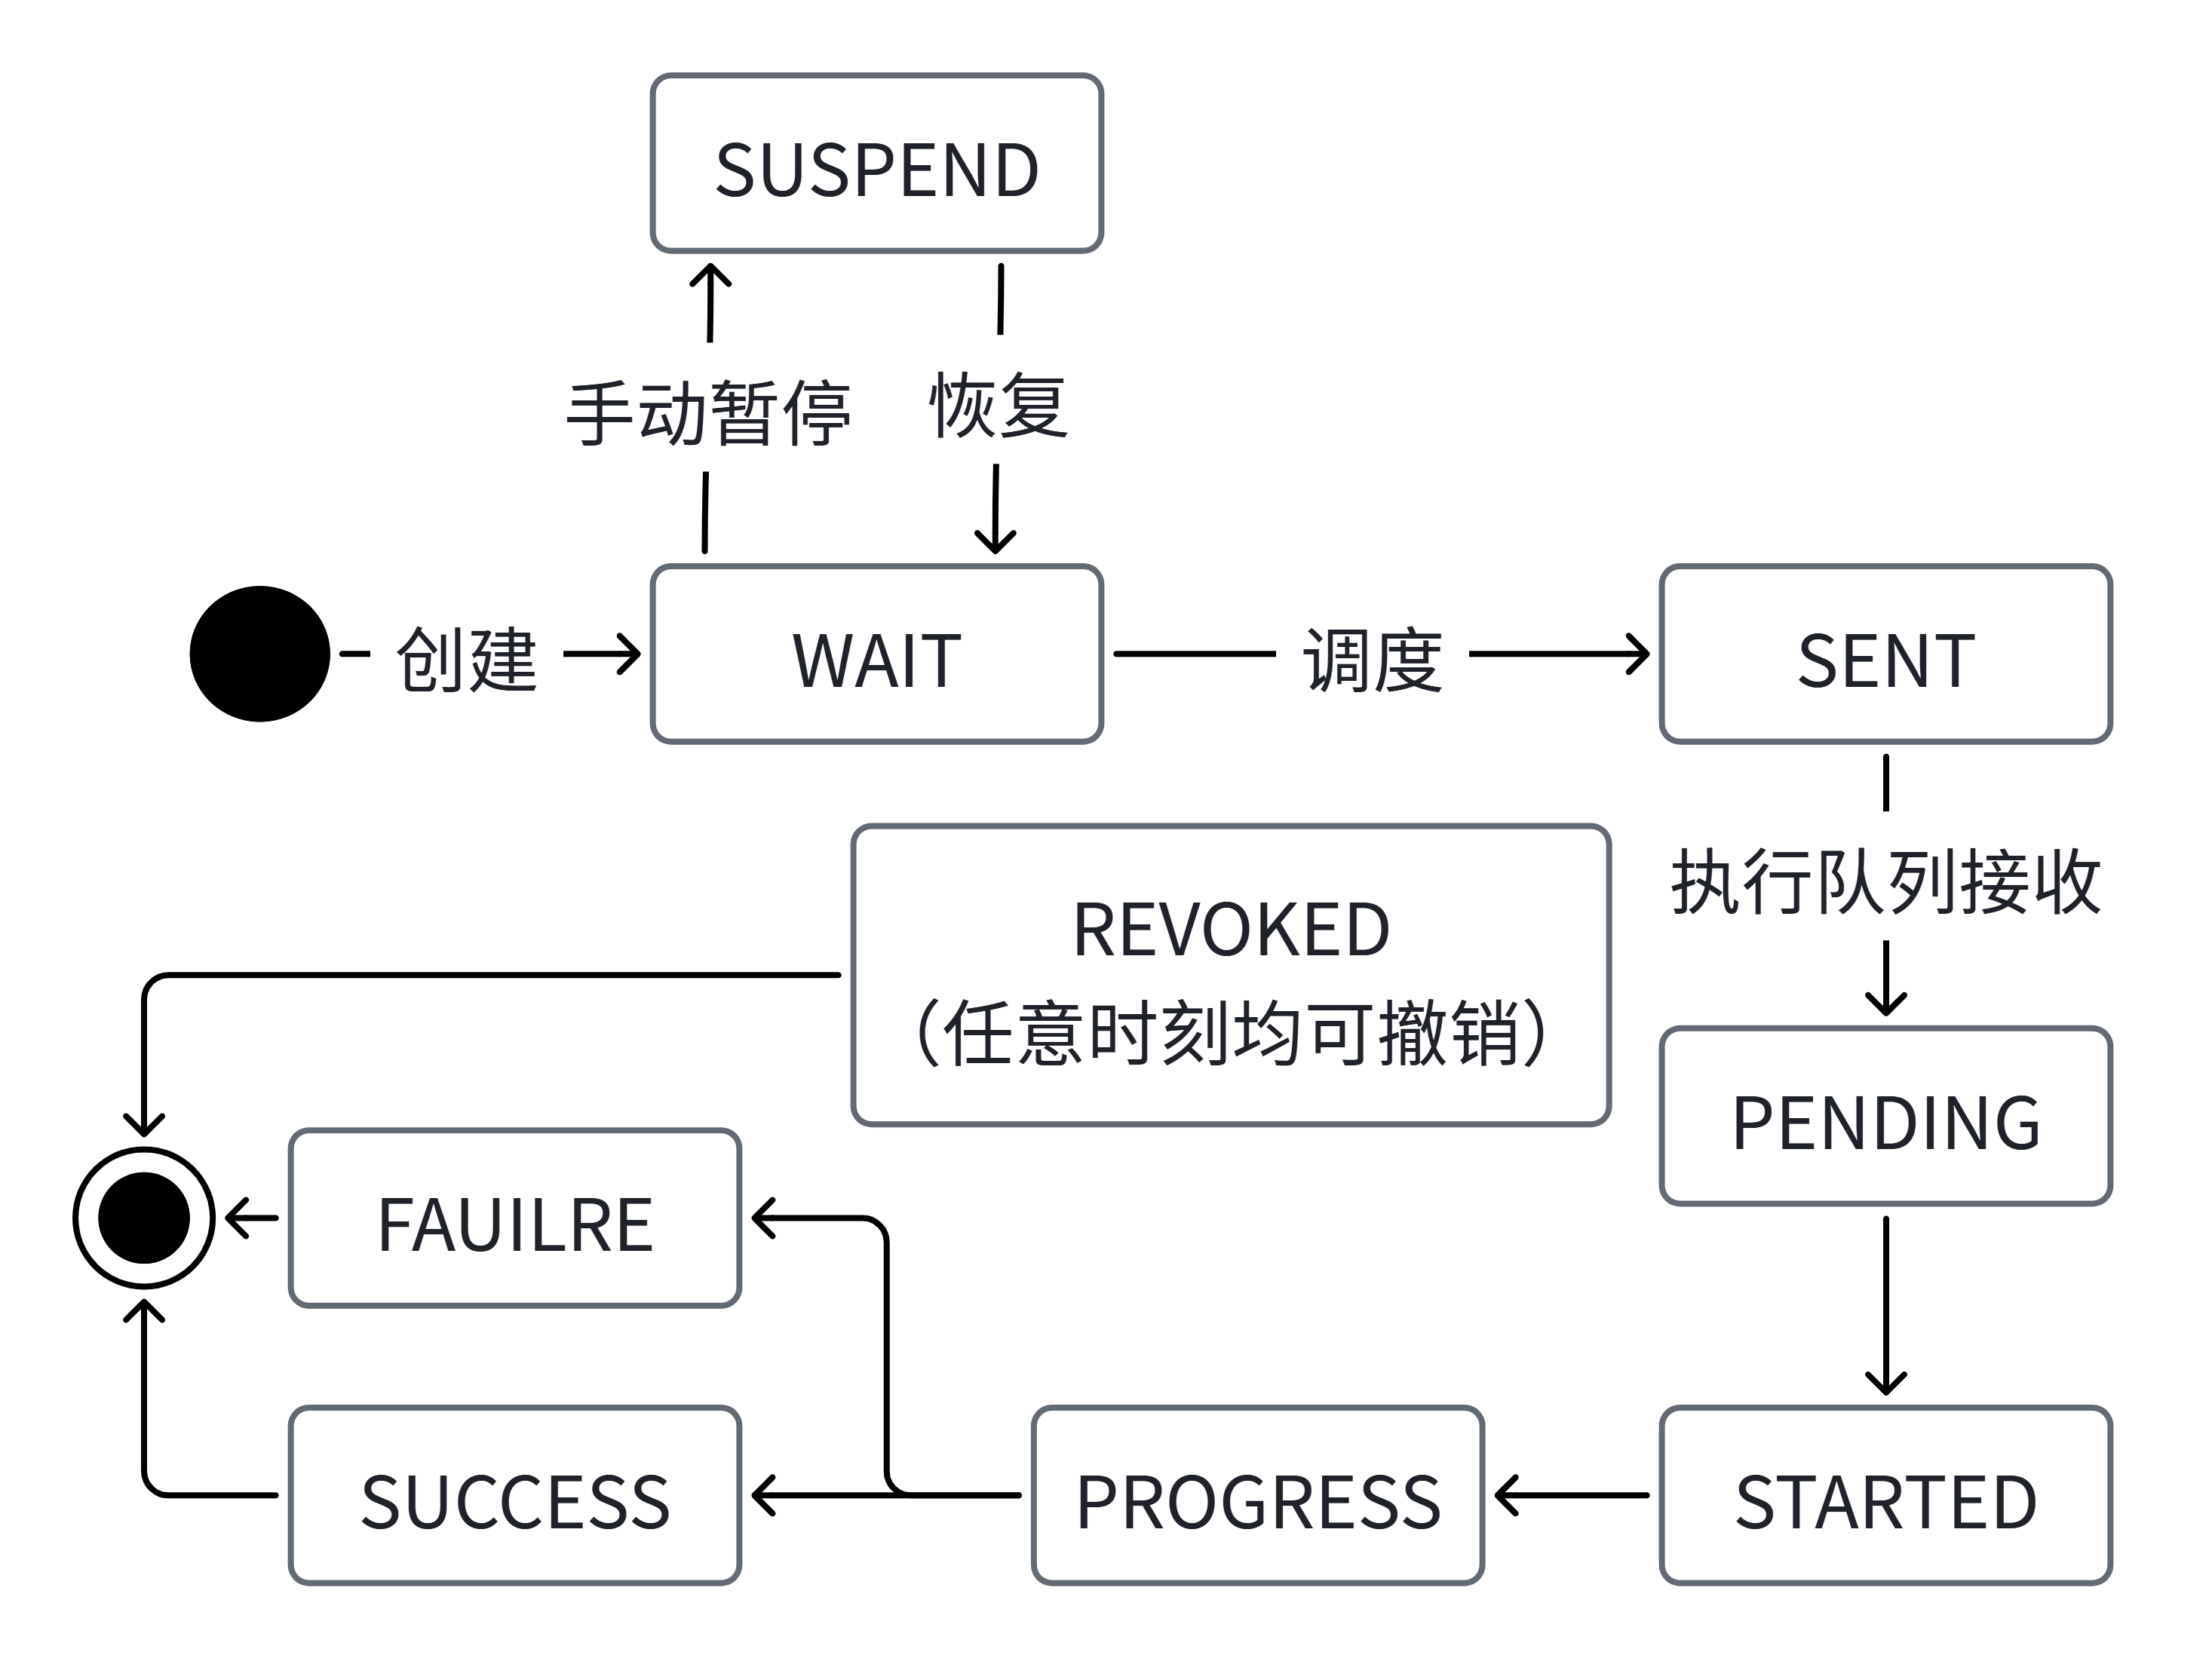
\includegraphics[width=0.8\linewidth]{figures/5/任务状态机.png}
    \caption{任务状态机}
    \label{fig:enter-label}
\end{figure}

\begin{figure}[htbp]
    \centering
    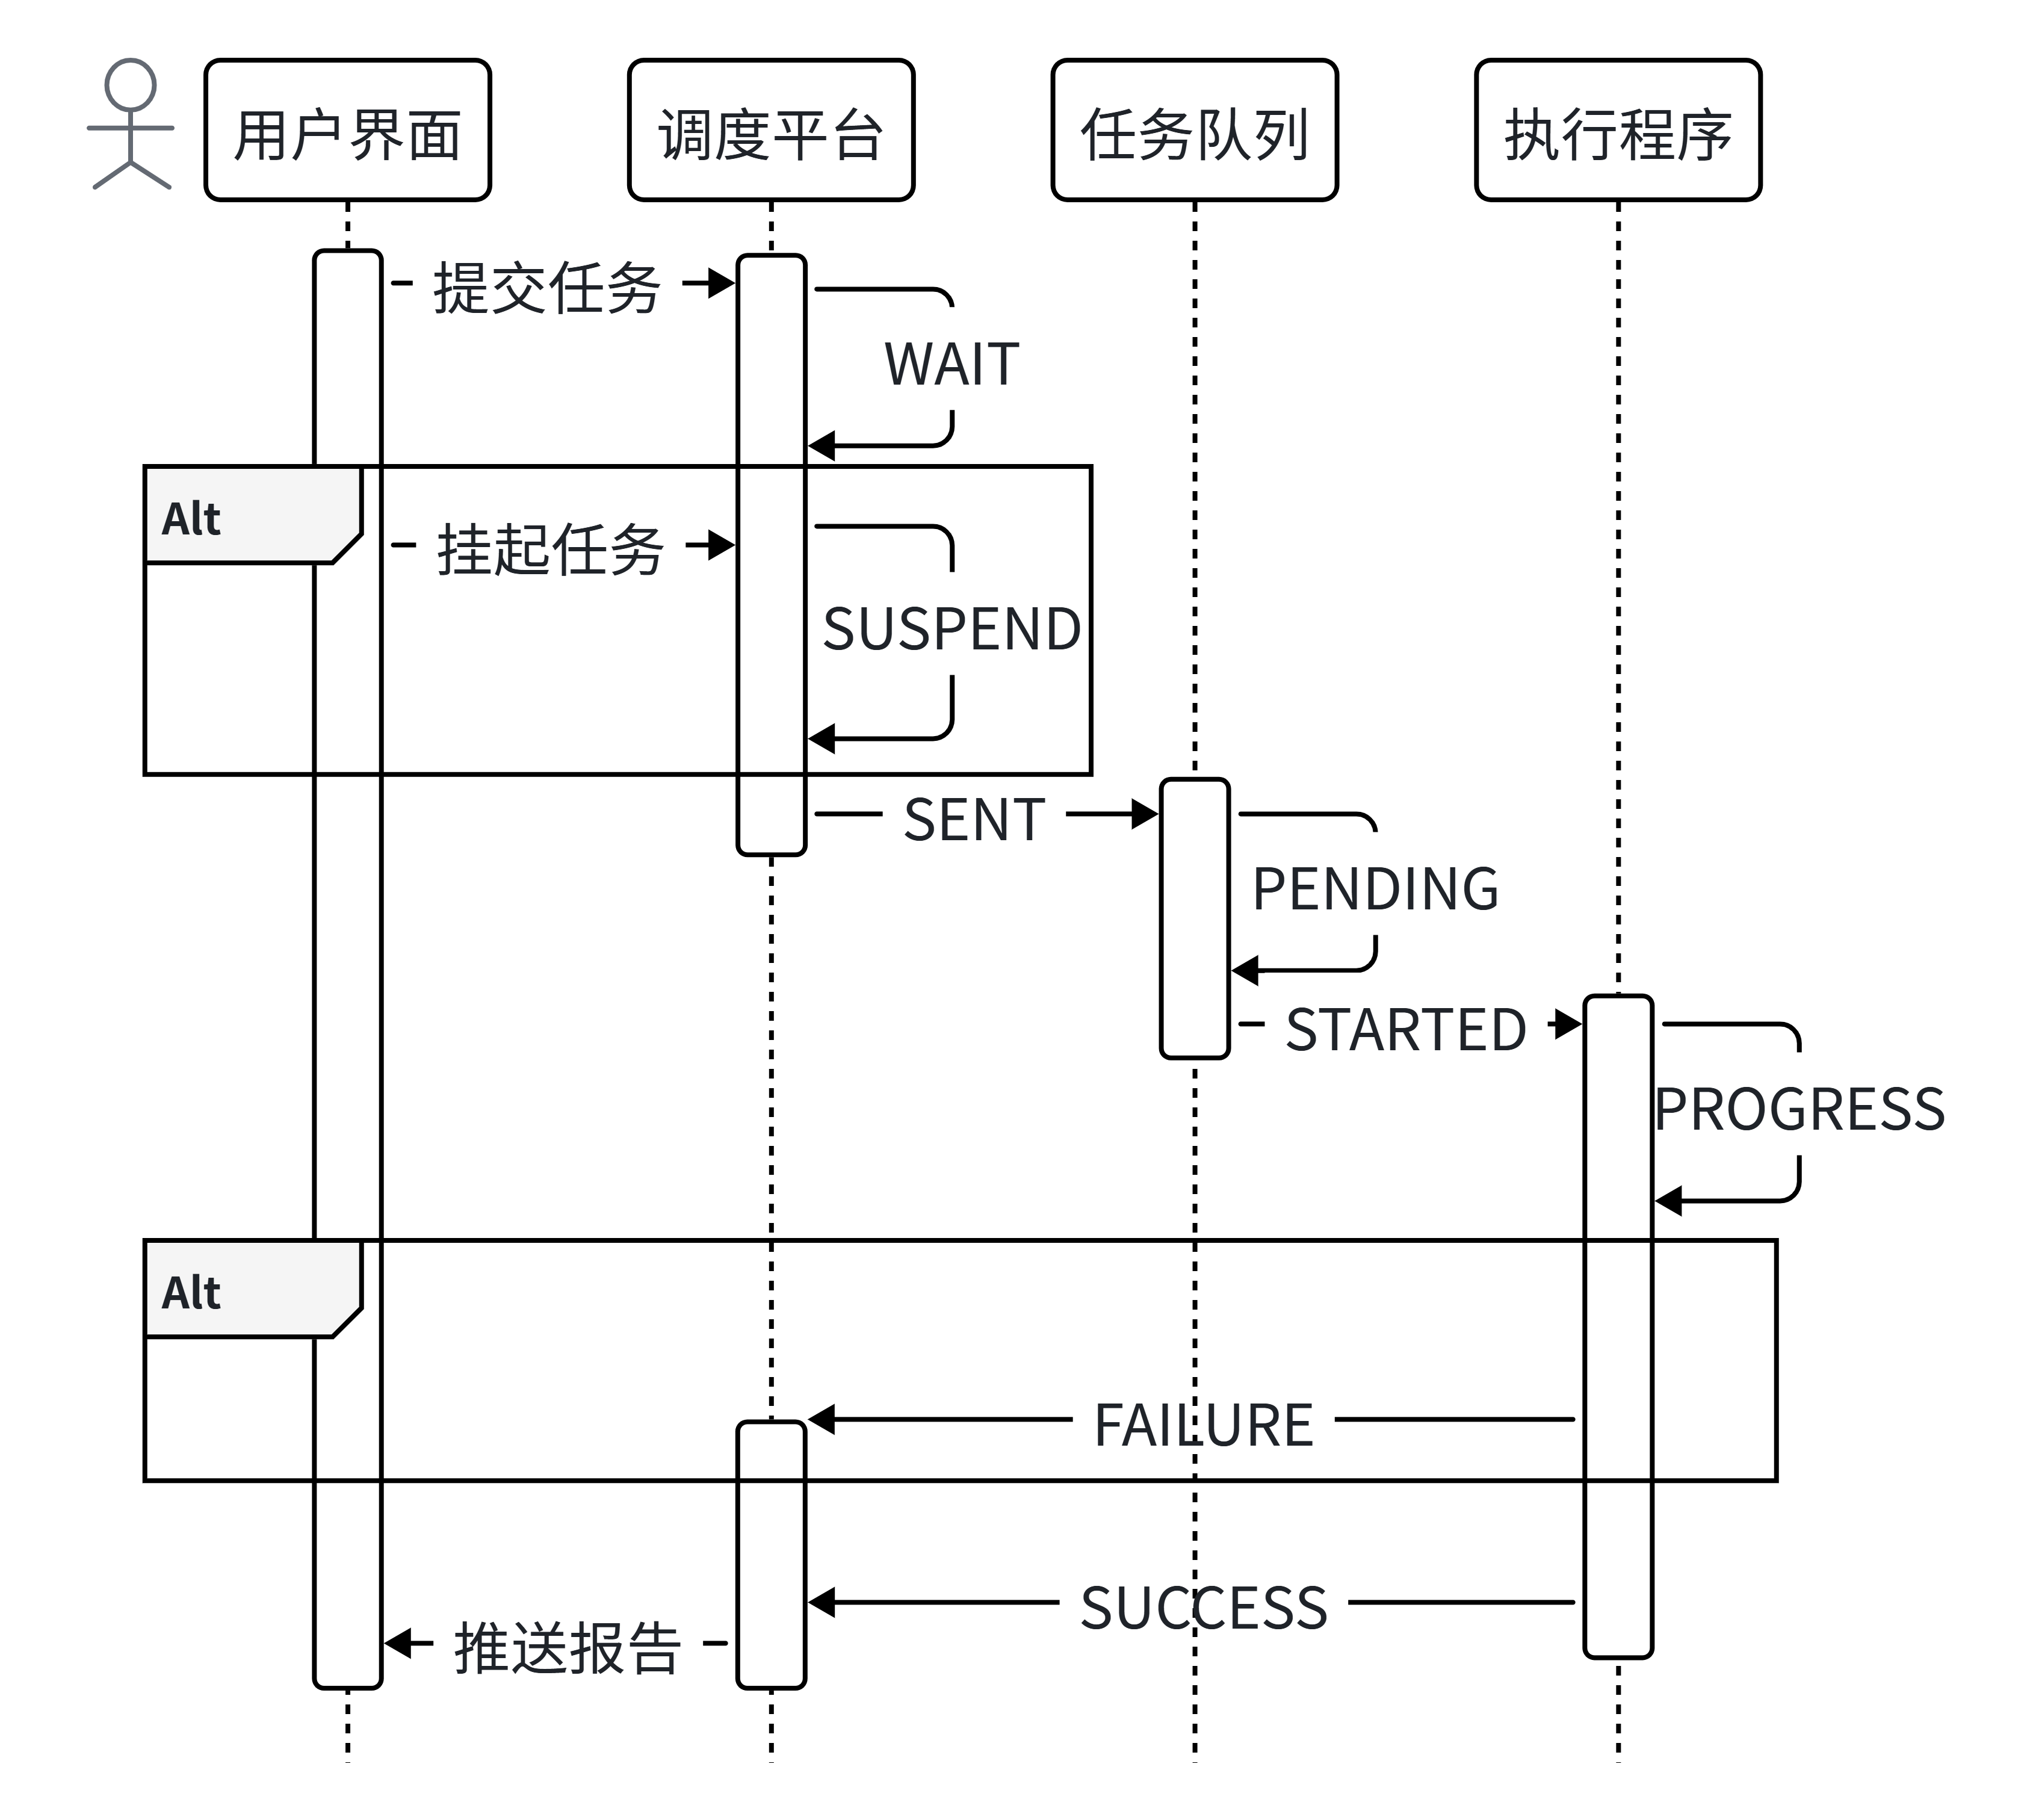
\includegraphics[width=0.8\linewidth]{figures/5/状态机时序图.png}
    \caption{状态机时序图}
    \label{fig:enter-label}
\end{figure}

\subsection{任务可用性检测}

本机制的设计与实现旨在攻克调度决策过度依赖人工判断的瓶颈。其研发过程经历了由静态硬编码向动态配置化逻辑引擎的演进：初期方案由于需求边界模糊，采用硬编码方式实现逻辑判断，缺乏灵活性；随着研究深入，本系统通过对多维业务场景进行需求调研与特征提取，构建了基于配置驱动的通用逻辑引擎。该设计允许管理员在不触动核心代码的前提下，通过修订策略配置文件即可实现调度逻辑的快速更迭。

任务可用性检测的核心在于构建一套具备环境感知能力的自动化决策体系。系统在调度周期内自动采集任务优先级、实时资源占用、环境兼容性等前置参数，并联动动态加载的策略规则进行多维度校验，最终自主输出“即时执行”或“挂队等待”的准入指令。从工程架构上看，逻辑引擎采用“解析-缓存-判定”的流水线模式。系统初始化阶段预先加载JSON格式的策略文件并将其序列化至内存规则库，在接收到调度请求时，引擎按“环境指标采集-策略规则匹配-准入结果判定”的逻辑链条执行自动化比对。这种配置驱动的架构设计，显著提升了系统在高动态AI研发环境下的扩展性与运维响应速度。

为实现复杂业务逻辑的标准化表达，本系统抽象出“条件”与“规则”两大核心算子。条件（Condition）： 逻辑判定的最小原子单元，用于评估特定环境下状态的真伪。每个条件由“编码（Code）”、“判断参数（Params）”及“固化逻辑”组成。其映射关系可表示为：
$$C = \{Code, Params\} \rightarrow f_{logic}(Env, Params)$$
其中，$Code$唯一标识底层判断逻辑，$Params$（如起始时间、负载阈值）则赋予同一逻辑适配不同场景的灵活性。规则（Rule）： 由原子条件经逻辑算子嵌套组合而成的复合表达式。本系统采用二级嵌套结构实现复杂的调度策略：一级数组元素间执行“或（OR）”逻辑，二级数组元素间执行“且（AND）”逻辑。其逻辑范式如下：
$$Rule = \bigvee_{i=1}^{n} \left( \bigwedge_{j=1}^{m} Condition_{i,j} \right)$$
这种结构支持高度灵活的策略表达，从而实现对异构任务的差异化准入控制。

针对多任务场景下的动态需求，系统建立了“任务-场景”双维度关联机制。每个任务类型绑定唯一任务编码及默认规则簇，而场景策略具备更高的决策优先级。调度引擎执行时，优先检索当前环境特征对应的场景规则。若场景规则命中，则优先执行场景约束；若无场景匹配，则回退至通用任务规则。这种优先级覆盖的机制，确保系统在节假日、算力峰值等特殊时空节点下，能够通过场景策略的实时注入，精准实现对AI多任务的智能流量分摊与风险规避。

任务可用性检测机制逻辑引擎的总体结构如图5.6所示。

\begin{figure}[htbp]
    \centering
    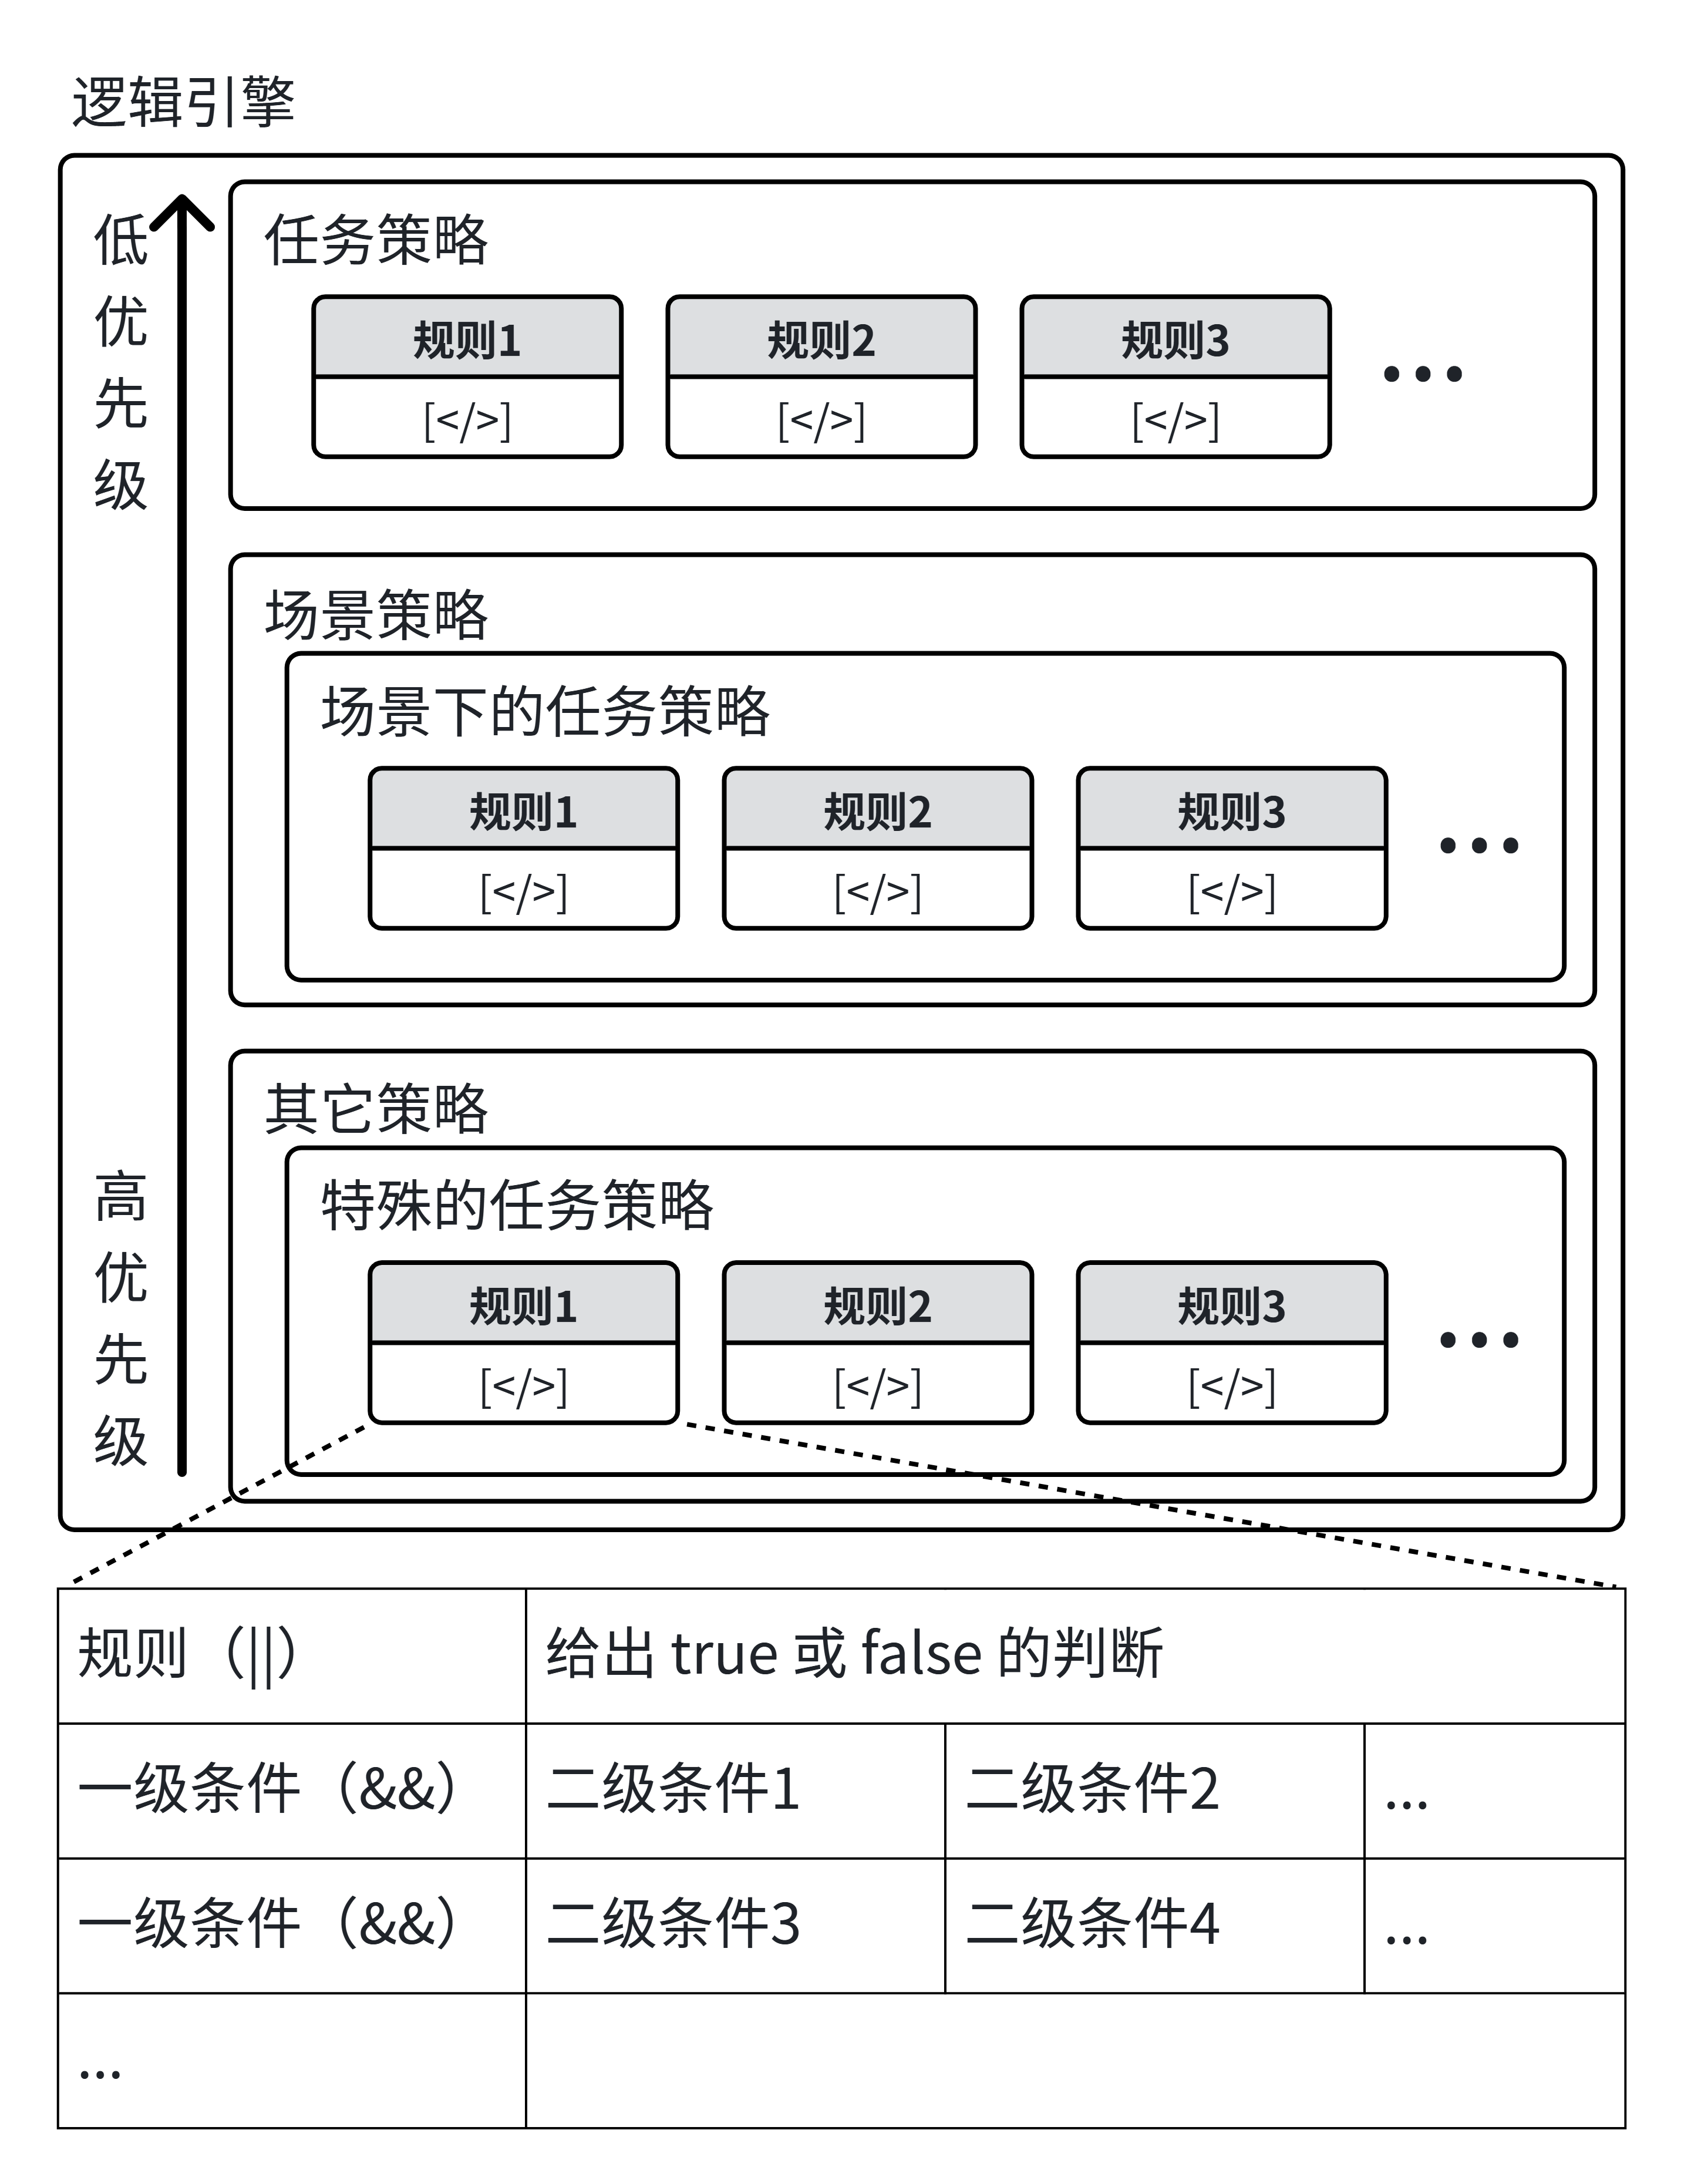
\includegraphics[width=\linewidth]{figures/5/逻辑引擎总体结构.png}
    \caption{逻辑引擎总体结构}
    \label{fig:enter-label}
\end{figure}

\subsection{资源可用性检测}

本机制的核心目标是解决子问题三中提到的“缺乏资源互斥智能分析能力导致的计算资源浪费”难题。在人工智能多任务场景下，GPU等算力资源通常具有强独占性。若调度算法无法精准识别不同任务间的资源依赖冲突，强行并发执行会导致显存溢出或计算数据冲突，进而造成任务失败与算力资源的严重空耗。因此，本机制通过构建细粒度的资源拓扑识别逻辑，实现了由“保守串行调度”向“高效并发调度”的转型。

从工程演进路径来看，资源可用性检测机制是系统实现“算力精细化治理”的关键跃迁。在系统研发初期，为保障核心框架的快速上线，调度逻辑侧重于基础任务流转；而在后续的迭代过程中，本系统通过三个版本的深度演进，逐步引入了动态资源锁机制与异步释放逻辑，使其能够灵活适配复杂异构场景下的临界资源约束。

\begin{table}[htbp]
    \centering
    \caption{资源占用表}
    \begin{tabular}{llllll}
        \toprule
        序号 & 字段名 & 字段说明 & 类型 & 是否可选 & 说明 \\
        \midrule
1 & task\_id & 任务ID & int & N &  \\
2 & resource\_id & 资源ID & int & N &  \\
3 & is\_delete & 此条记录是否有效 & boolean & N &  \\
4 & id & 本条记录id & int & N &  \\
        \bottomrule
    \end{tabular}
    \label{tab:my_label}
\end{table}

为支撑高效的互斥判定，系统建立了如表5.2所示的资源占用记录表。该表作为全局调度状态的“实时快照”，通过简洁的三元结构实现了任务与临界资源的高性能映射。该模型的设计逻辑在于：通过 task\_id 与业务任务表建立多对一关联，实现对单一任务多维度资源依赖的完整覆盖；利用 is\_delete 字段实施状态柔性管理，在任务撤销或异常终止时，系统通过逻辑删除实现算力资源的秒级释放，无需物理删除历史记录，既提升了数据库吞吐量，又为后续的算力使用审计提供了全量数据溯源支持。

资源可用性检测的操作逻辑通过“静态注册-动态探测-准入控制”的闭环流程，实现了对AI临界资源的精细化治理，从技术底层化解了算力冲突难题：

\begin{enumerate}
    \item 资源注册：任务编写者需根据AI算子的具体执行特征（如是否涉及独占性GPU显存、特定硬件加速器等），在任务定义阶段预先声明其所需的临界资源清单。这一步骤通过元数据建模，将抽象的任务需求转化为系统可感知的资源需求矩阵，为后续的互斥分析提供了静态参考基准。
    \item 状态探测：调度引擎在触发任务下发逻辑前，会执行原子化的探测操作，实时扫描数据库中的资源占用表。系统通过检索目标资源对应的 is\_delete 标识位，判定该资源是否处于“逻辑锁定”状态。若探测到目标资源已被其他活跃任务占用，系统将精准识别此次调度动作为“互斥冲突”，并记录冲突拓扑以备后续调度参考。
    \item 并发决策：针对识别出的互斥任务，系统采取非阻塞式的“延迟重试”策略，将其自动挂起至高可靠等待队列，避免了暴力重试引发的算力波动。而对于经探测判定为资源相互独立的任务，调度引擎则打破传统的串行执行模式，在验证任务可用性后立即触发并发执行。这种基于资源感知的动态分流机制，极大缩短了任务间的间隙空耗，显著提升了异构计算集群的整体吞吐性能。
\end{enumerate}

这种基于细粒度资源感知的设计，有效打破了传统系统中由于调度盲区导致的串行执行瓶颈，最大化了多任务环境下的系统吞吐量。具体的互斥判断机制流程如图5.7所示。

\begin{figure}[htbp]
    \centering
    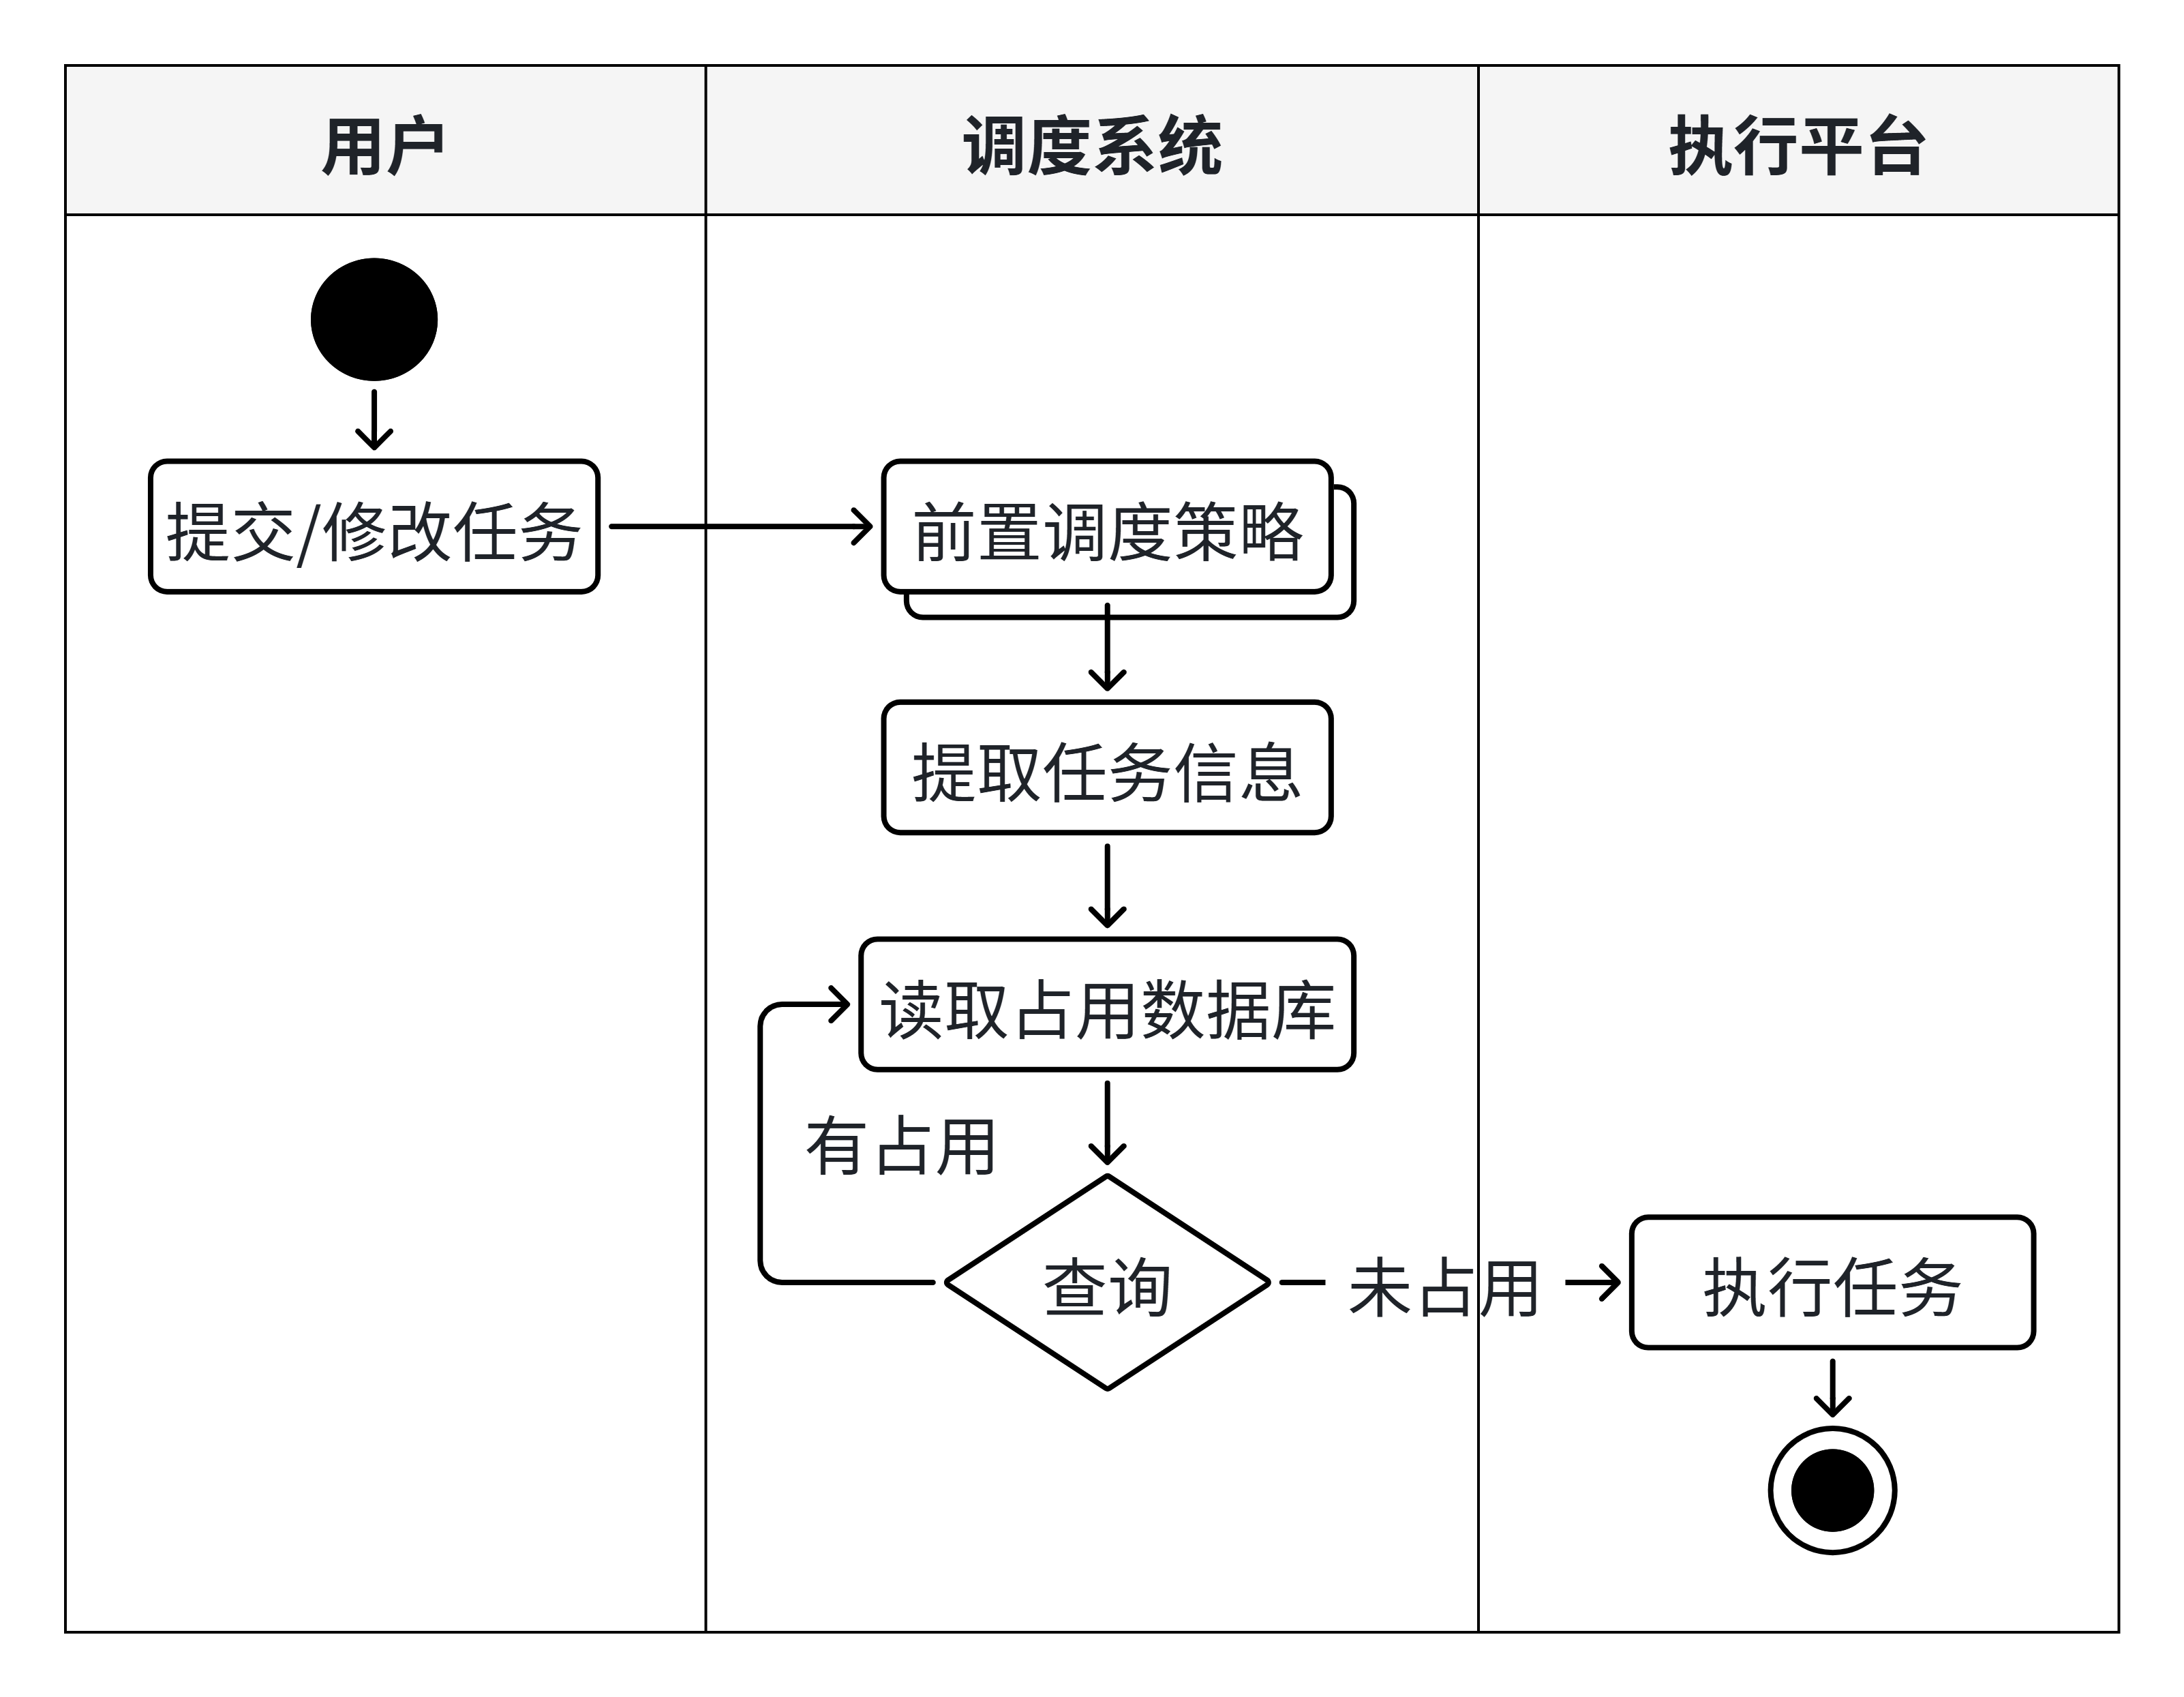
\includegraphics[width=\linewidth]{figures/5/资源互斥判断机制.png}
    \caption{资源互斥判断机制泳道图}
    \label{fig:enter-label}
\end{figure}

资源互斥判断机制，作为核心算法的一部分，与任务可用性检测互相配合，共同保障本系统的资源分配、任务运行、数据流转的正确性。

\subsection{负载均衡及性能优化设计}

本系统部署于公司内部，架构包含中心调度程序以及任务执行节点。鉴于不同开发组在预算与需求方面存在差异，其配备的任务执行节点在性能与容量上也会有所不同，因此无法采用统一的调度策略对这些节点进行管理。

在考虑云计算时，负载均衡方法的核心在于在不同的虚拟机之间分配工作负载\cite{gudivada2025}。NGINX作为业内极具领先地位的高性能HTTP服务器，其内部搭载了性能卓越的权重轮询算法，可以将请求分散到体系内的多个虚拟机上，实现了出色的负载均衡\cite{nikishin2022}。该算法凭借出色表现，在众多公司及多个领域获得了广泛应用与高度信赖。鉴于此，本系统的负载均衡算法在一定程度上借鉴了NGINX的Weighted Round Robin算法，实际上是该算法的一个简化版本。

节点通过类型与权重进行注册：类型决定任务匹配，权重表征执行能力。同一类型的节点组成“本地列表”，系统通过加权轮询算法进行调度。在单次轮询中，系统会根据权重值n在该节点连续分配n次任务后切换。该机制确保了节点的高效负载均衡，且管理员可通过将权重设为 0 实现节点的逻辑禁用。其原理如图 5.8 所示。

\begin{figure}[htbp]
    \centering
    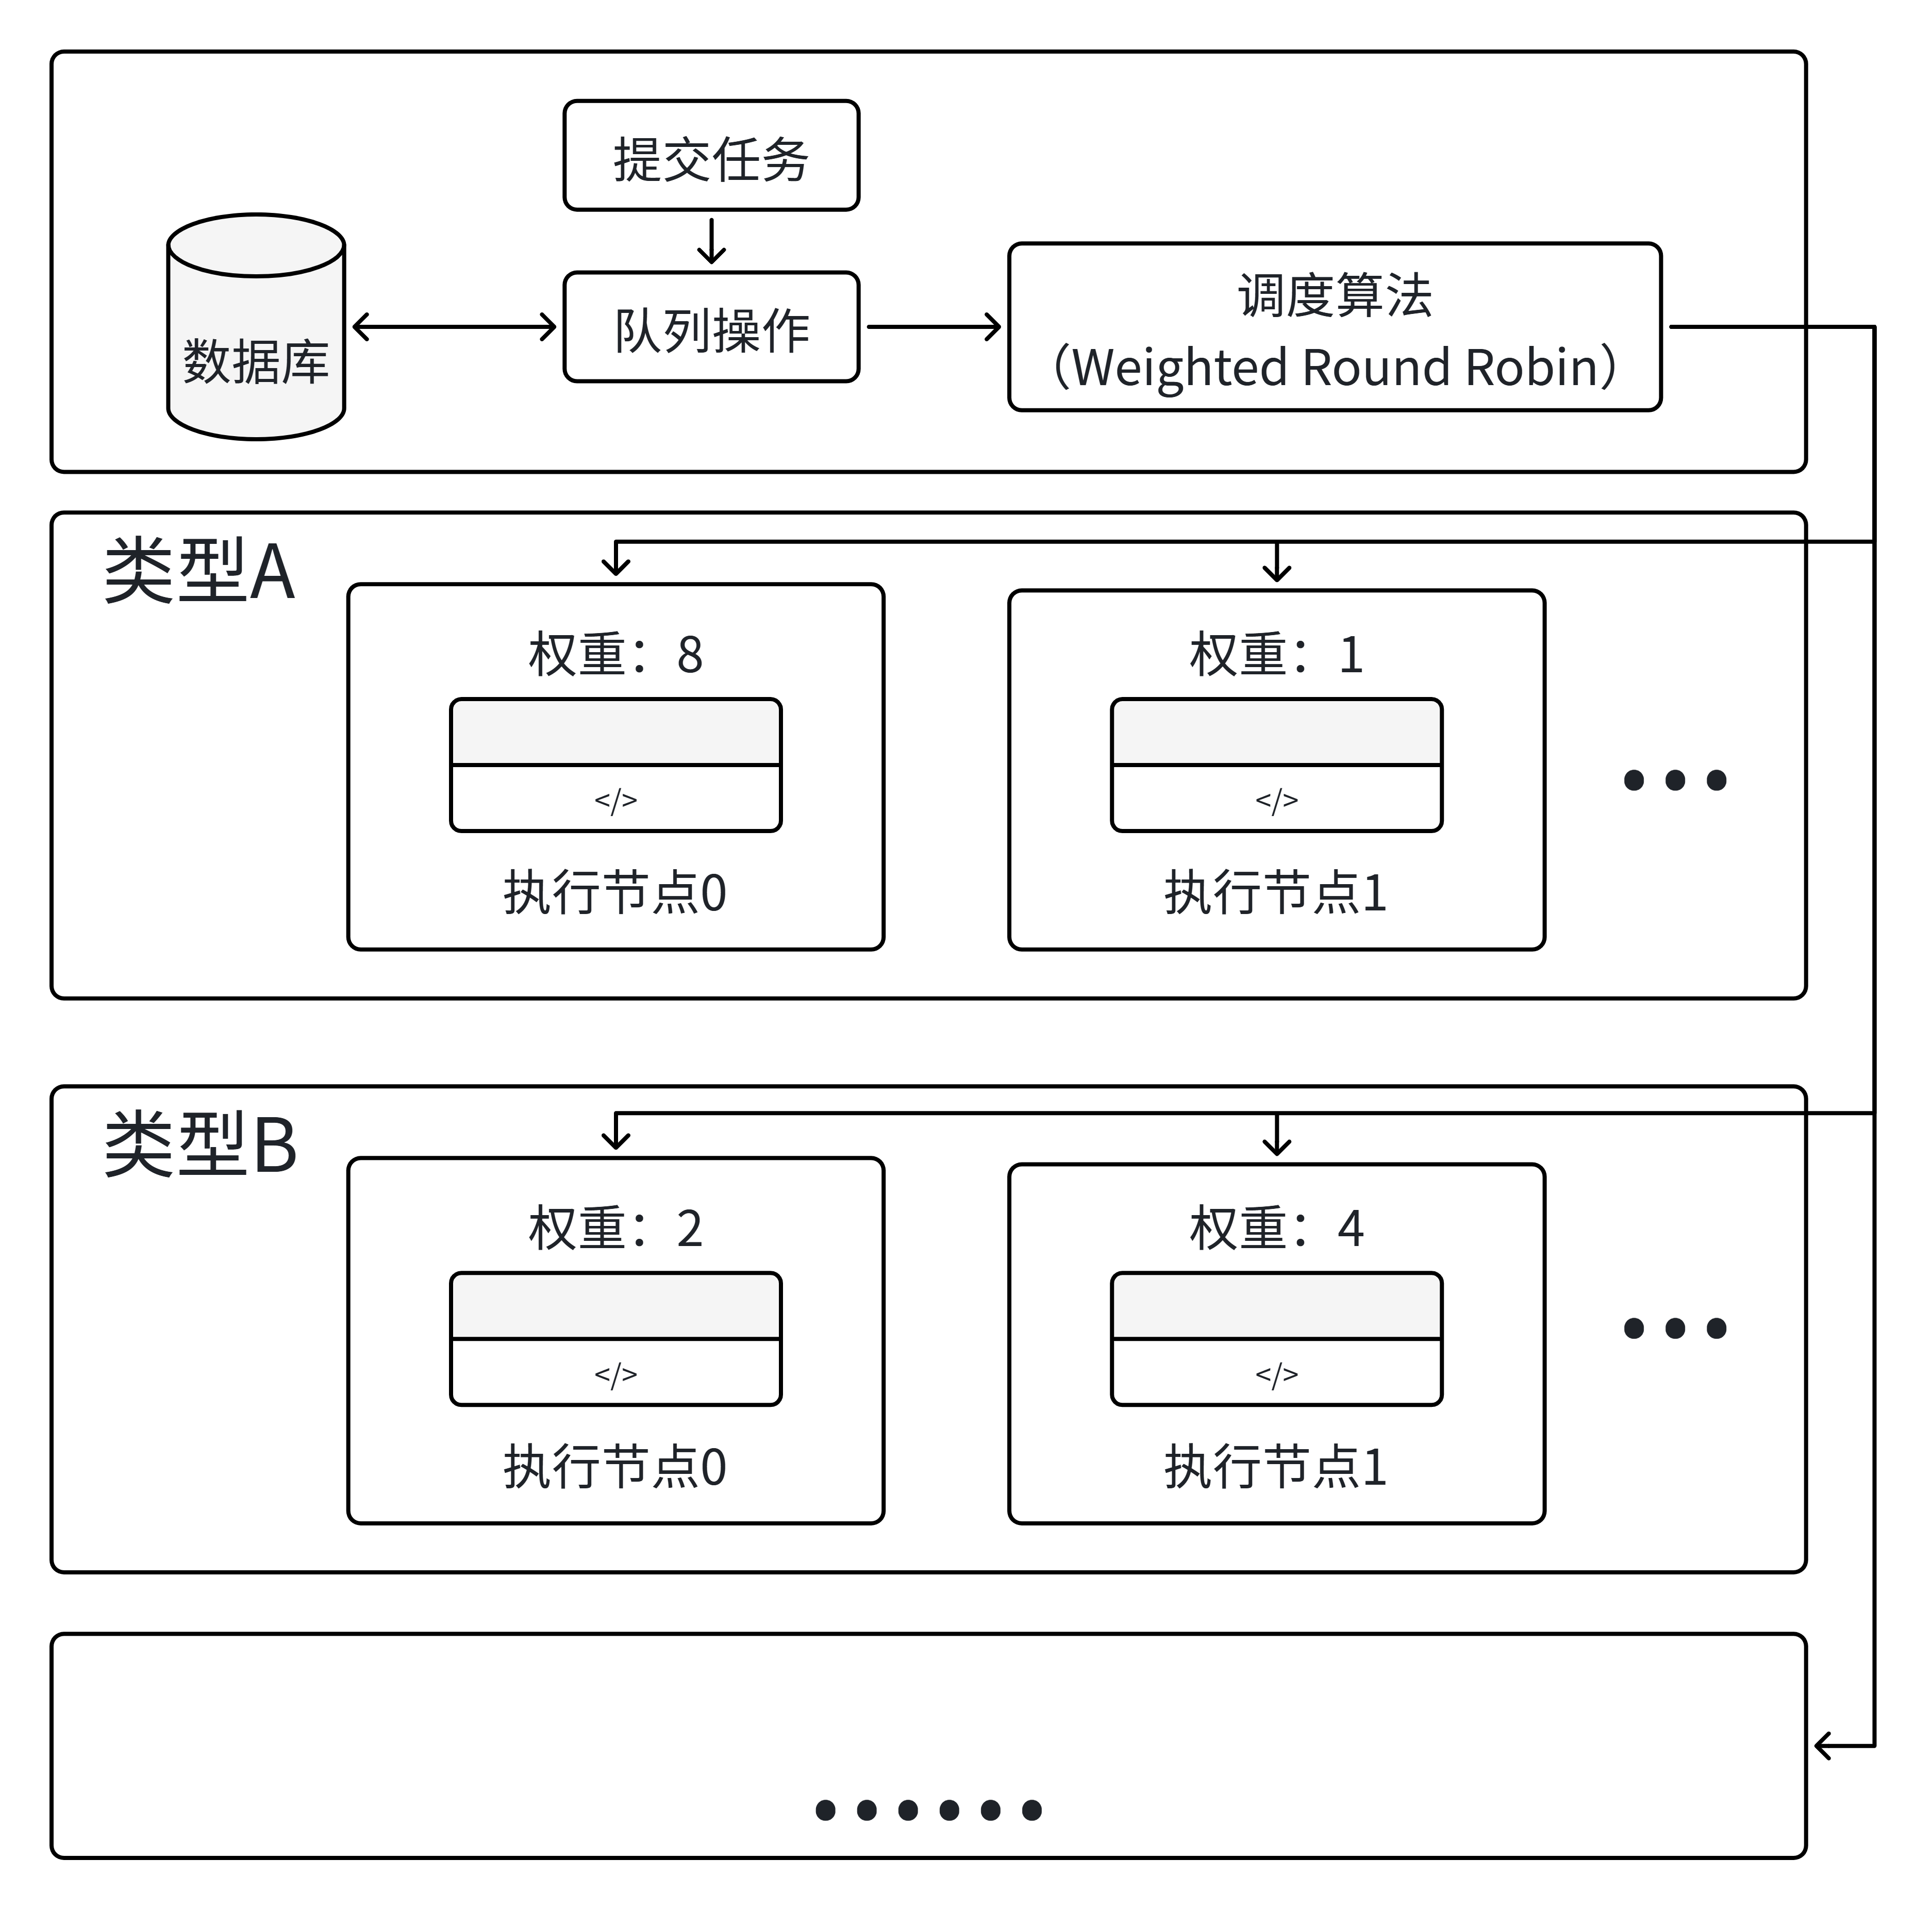
\includegraphics[width=\linewidth]{figures/5/负载均衡示意图.png}
    \caption{负载均衡原理图}
    \label{fig:enter-label}
\end{figure}

\subsection{数据同步模块}

本系统采用分布式微服务架构，由多个执行节点共同提供算力支撑。针对多模块环境下信息交互易冲突、协同效率低的痛点，系统专门设计了一套高可靠的数据同步机制。该机制通过标准化的通信链路，实现了AI任务参数与状态数据的透明流转，确保调度指令能精准下发、执行进度能实时回收，为系统实现自动化决策和资源精细化管控提供了关键的数据纽带。

在技术落地层面，系统选用Redis作为核心消息中间件，并依托Celery分布式框架实现任务的异步解耦。任务调度层会将校验纠错后的AI任务及其异构参数封装并存入Redis任务队列；执行节点作为客户端实时监听并领用任务，解析Prompt、资源列表等关键参数后，调用本地算子开展计算。任务执行完毕，节点会通过Celery将结果写回Redis。调度中枢捕获状态变更后，会即时更新本地数据库并反馈至前端，确保操作员能实时监测任务的运行状态与资源占用，彻底解决了过去由于信息流转不畅、过度依赖人工介入导致的系统效率低下问题。

数据同步模块的原理如图5.9所示。

\begin{figure}[htbp]
    \centering
    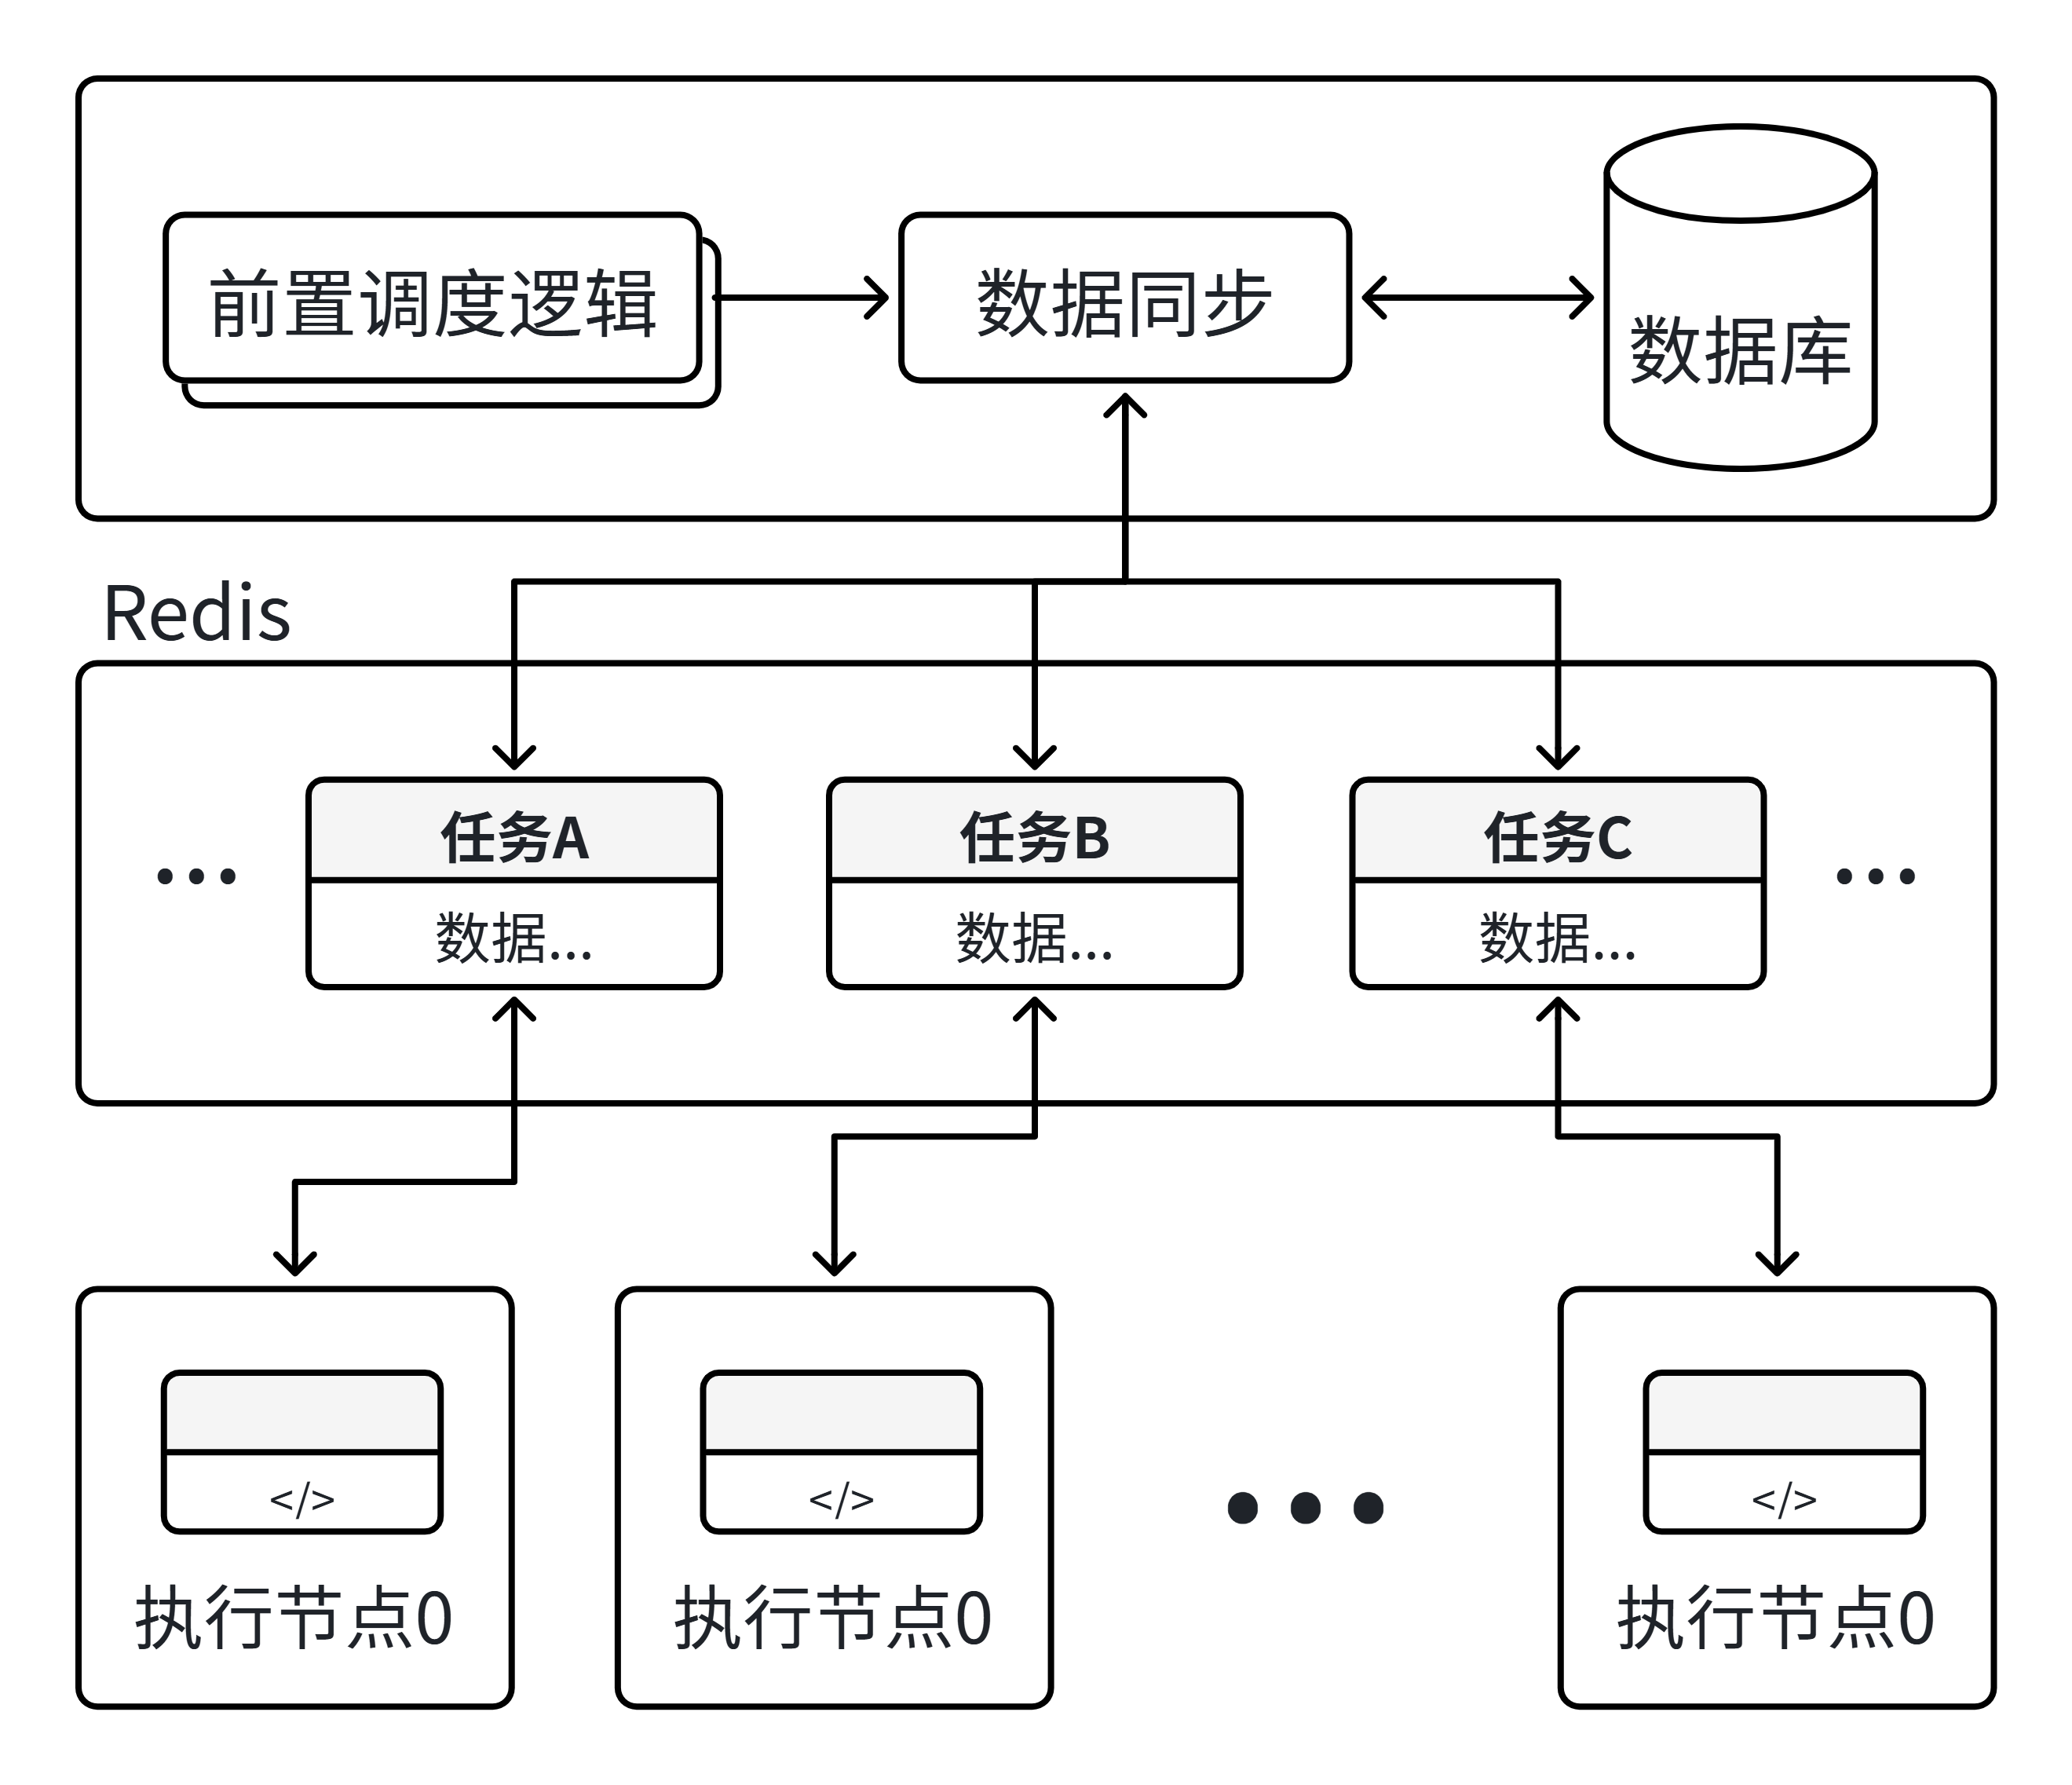
\includegraphics[width=\linewidth]{figures/5/数据同步模块原理图.png}
    \caption{数据同步模块原理图}
    \label{fig:enter-label}
\end{figure}

\subsection{容错与恢复机制}

本系统针对AI多任务场景下高算力消耗、执行周期长的特征，设计了一套具备环境感知能力的故障自愈机制。由于AI任务在执行过程中极易受到底层计算环境（如容器资源限制、网络波动等）的干扰导致异常中断，传统的调度模式往往需要操作员介入重提任务，造成了极高的人力和算力成本浪费。为此，系统通过构建全生命周期的指标监测体系，实现了对非致命性错误的自动化识别与闭环治理，旨在消除调度决策对人工干预的依赖，从底层保障算力资源的持续高效周转。

在技术落地层面，系统针对四类典型场景构建了精细化的自愈策略：首先，针对k8s环境下的CPU超限，系统在检测到限流抖动后会自动调低调度并发度，确保核心服务的可用性；其次，利用Python异常捕获机制识别内存不足（OOM）报错，系统会将受影响任务重置为等待状态并自动重回队列，待资源水位回落后执行异步调度，且支持最多三次的静默重试逻辑，重试间隔按照指数退避策略进行，三次重试均失败后，按照“执行失败”标记并推送面板，随即释放资源；再次，针对AI长周期任务中常见的文件描述符堆积，系统建立了实时监控与阈值预警机制，防止潜在的句柄泄露引发系统级崩溃；最后，面对网络抖动导致的API超时，系统内置了基于指数退避算法的重试策略，在保障任务执行韧性的同时有效规避了请求雪崩。通过这套多级容错体系，系统成功实现了从“人工排障”向“引擎自愈”的智能化转型。

\section{任务执行层详细设计}

作为系统算力落地的最终环节，任务执行层直接决定了AI多任务调度的响应质量与数据鲁棒性。针对现有系统在AI特性适配上的不足，本层通过构建标准化的路由分发机制与算子执行单元，确保调度中枢下发的智能化指令能精准转化为具体的算力输出。它不仅承担了繁重的异构数据处理工作，还与监控平台深度联动，通过对执行过程的实时感知，实现了从“参数流入”到“结果反馈”的全流程自动化管理，有效解决了因子模块环境差异导致的任务执行瓶颈。

路由模块在接收到调度平台下发的指令后，首先会启动关键的“环境初始化”程序。这一阶段不仅涵盖了针对大模型任务的异构数据映射，还深入涉及了模型参数的本地化预处理与张量对齐，旨在从执行端彻底化解子问题一中描述的多源异构适配难题。环境就绪后，路由模块将结合实时生成的任务画像（如算子偏好、显存预估等指标），动态挑选出最契合当前计算需求的执行算子，并正式驱动该算子开启高强度的AI计算任务。在任务运行的整个周期内，监控平台会建立高频采样通道，实时收集并统计算力节点的各项关键数据。系统能够精准捕获CPU利用率、显存带宽占用以及能耗分布等临界资源的动态变化，并将这些原始遥测数据转化为结构化的分析结果，实时反馈给路由模块以生成精炼的执行简报。最后，系统会将这份包含任务实时进度、性能水位线及异常拦截记录的简报同步至调度平台，从而在底层执行与上层调度之间形成了一个完整的状态反馈闭环。这种机制彻底告别了传统模式下依赖人工干预来监控任务状态的低效方式，使得大模型任务的整个执行过程在实现自动化流转的同时，变得既高效又透明。

具体的执行流程如图 5.10 所示。

\begin{figure}[htbp]
    \centering
    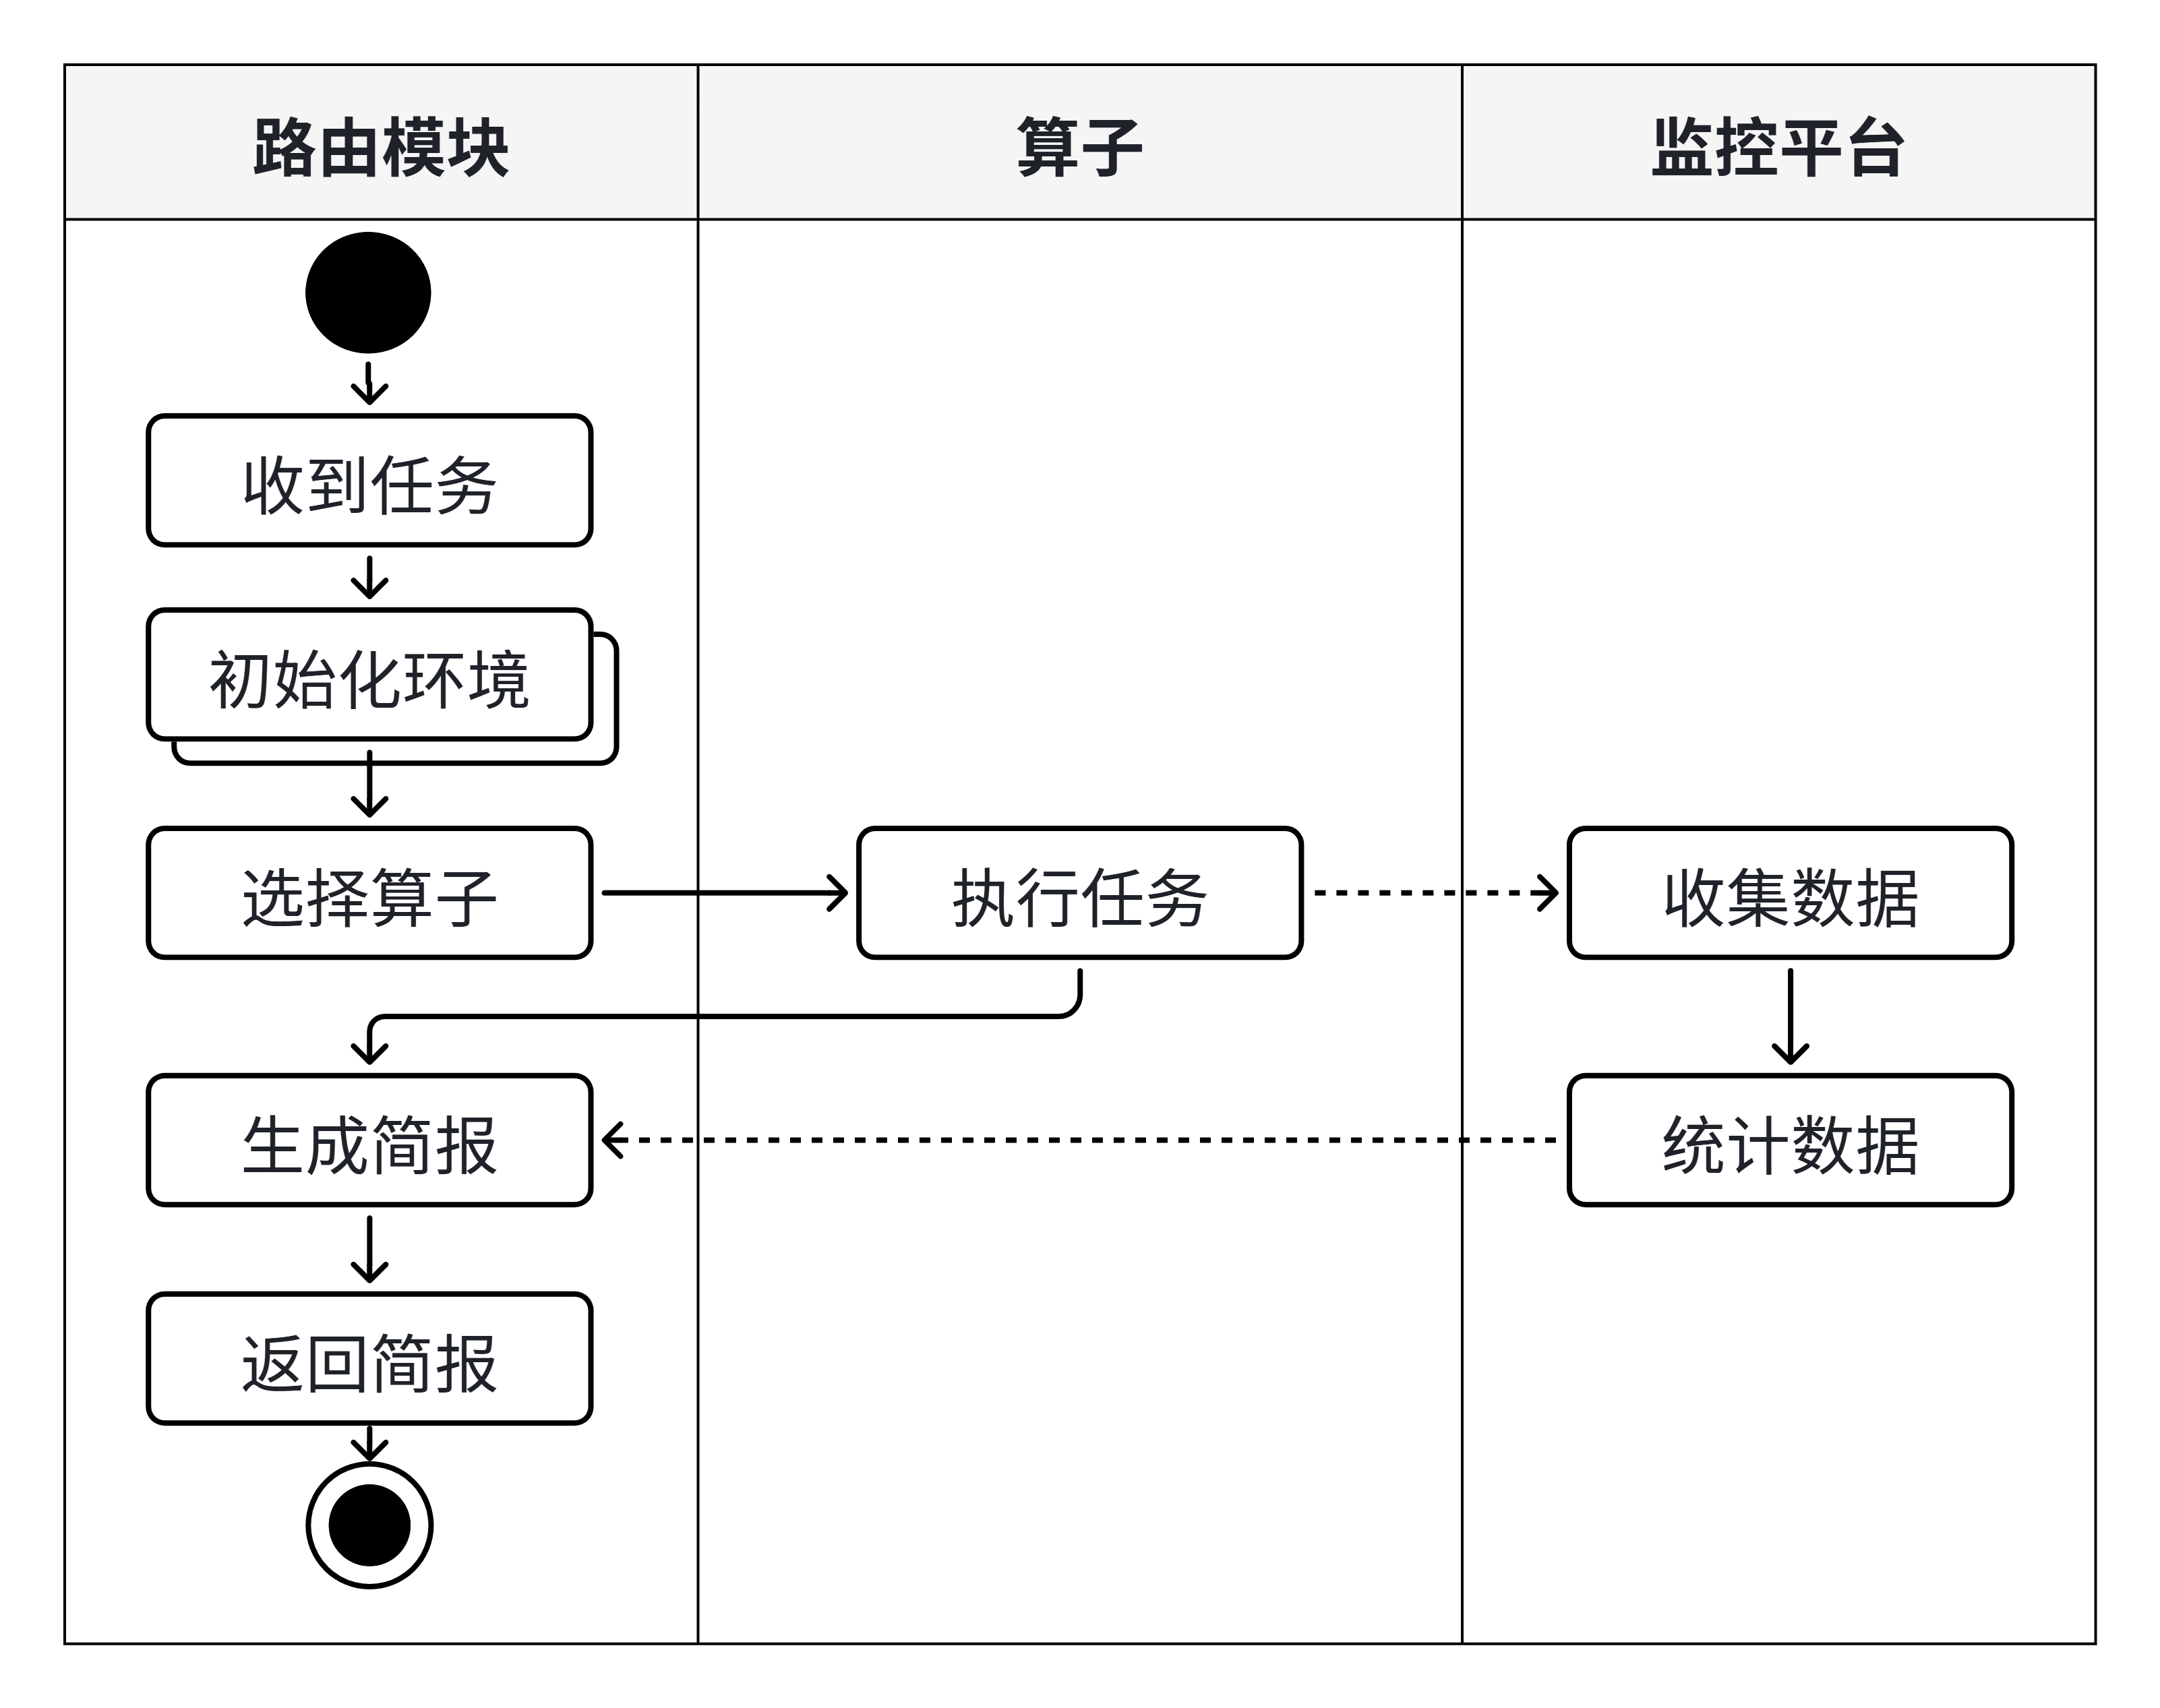
\includegraphics[width=\linewidth]{figures/5/任务执行流程.png}
    \caption{任务执行泳道图}
    \label{fig:enter-label}
\end{figure}

\subsection{参数传递约定}

本系统通过构建基于JSON与Python字典（dict）的深度映射机制，实现了AI异构参数在分布式环境下的透明流转。针对大模型任务参数多样、结构复杂的特性，这一设计充分发挥了Python生态与Celery框架在数据处理上的灵活性，从底层打通了前端面板、数据库与执行节点之间的信息链路。通过将非结构化的请求精准解析为逻辑层可识别的执行对象，系统不仅有效提升了对异构数据的处理兼容性，也为后续实现复杂的自动化调度决策奠定了统一的数据基准。

在具体实现细节上，系统规定了一套涵盖任务标识、资源链路及存储路径的基础参数协议。其中，resource\_url字段支持对AI依赖附件的自动化关联，而output\_dir与log\_dir则由系统根据任务画像自动生成并定向，彻底消除了过去需要程序员手动配置路径、预建目录的机械劳动，有效避免了因路径配置错误而导致的启动失败问题。此外，系统内置了参数合法性校验与运行环境自愈逻辑，在任务启动前会自动初始化物理目录，确保执行环境的一致性；在任务结束后，则会即时触发冗余数据清理机制，避免历史文件堆积对集群存储造成持续压力。这种从“自动创建”到“按需回收”的全流程管理模式，不仅显著降低了因子模块配置偏差导致的任务崩溃风险，也极大优化了算力集群的存储空间周转效率，为大规模任务的稳定调度奠定了可靠的基础设施支撑。参数传递约定如表5.3所示。

\begin{table}[htbp]
    \centering
    \caption{任务基本参数}
    \begin{tabular}{llllll}
        \toprule
        序号 & 字段名 & 字段说明 & 类型 & 是否可选 & 说明 \\
        \midrule
1 & task\_id & 任务ID & int & N &  \\
2 & celery\_id & Celery ID & int & N &  \\
3 & resource\_url & 所依赖资源链接 & string & Y & 任务可无附件 \\
4 & output\_dir & 任务输出文件路径 & string & N &  \\
5 & log\_dir & 任务日志路径 & string & N &  \\
        \bottomrule
    \end{tabular}
    \label{tab:my_label}
\end{table}

\subsection{任务编辑方式}

在AI大模型的研发迭代中，任务代码绝非一劳永逸，往往需要根据业务逻辑的演进或模型参数的调整进行动态修正。本系统针对传统模式下代码更新链路长、易出错的痛点，构建了一套涵盖“编辑、提交、审核、上线”四大环节的敏捷闭环机制。该机制旨在为操作员提供一条自动化的代码变更流水线，确保在保障系统运行环境一致性的前提下，能够快速、准确地修正业务逻辑。这不仅解决了手动更新带来的环境适配难题，也通过标准化的流程审计，进一步减少了由于代码误操作导致的算力资源空耗，为实现调度决策的自动化提供了可靠的逻辑底座。

在具体工程实现上，代码变更流程被赋予了极强的容错与安全属性。操作员在完成代码针对性修订的同时，系统会同步采集配套的依赖库信息，通过自动化构建保障执行端环境的无偏差映射，确保开发环境与生产环境在依赖层面保持严格一致，从根本上杜绝了因“本地跑得通、线上崩了”引发的执行异常。为了筑牢安全防线，系统引入了管理员审计机制，所有待发布的代码变更与依赖更新均需经过管理员的严格审查与确认，通过对逻辑变更与依赖更新的双重审核，有效拦截潜在的运行风险。一旦审核通过，全自动分发引擎会即时将新代码推送到分布式执行节点，实现业务逻辑的无感升级，整个过程对正在运行的任务无任何干扰。更为关键的是，系统依托Git技术设计了线性版本管理策略，为每一次代码更替配置了“一键回滚”的兜底手段。当新代码出现非预期行为时，操作人员可迅速撤回至历史稳定版本，将故障影响控制在最小范围内。这种“自动化部署+版本化隔离”的设计，不仅解决了AI多任务场景下的频繁迭代难题，也极大提升了系统的整体韧性与运维效率，为持续交付提供了可靠的技术保障。任务编辑的垂直泳道图如图5.11所示。

\begin{figure}[htbp]
    \centering
    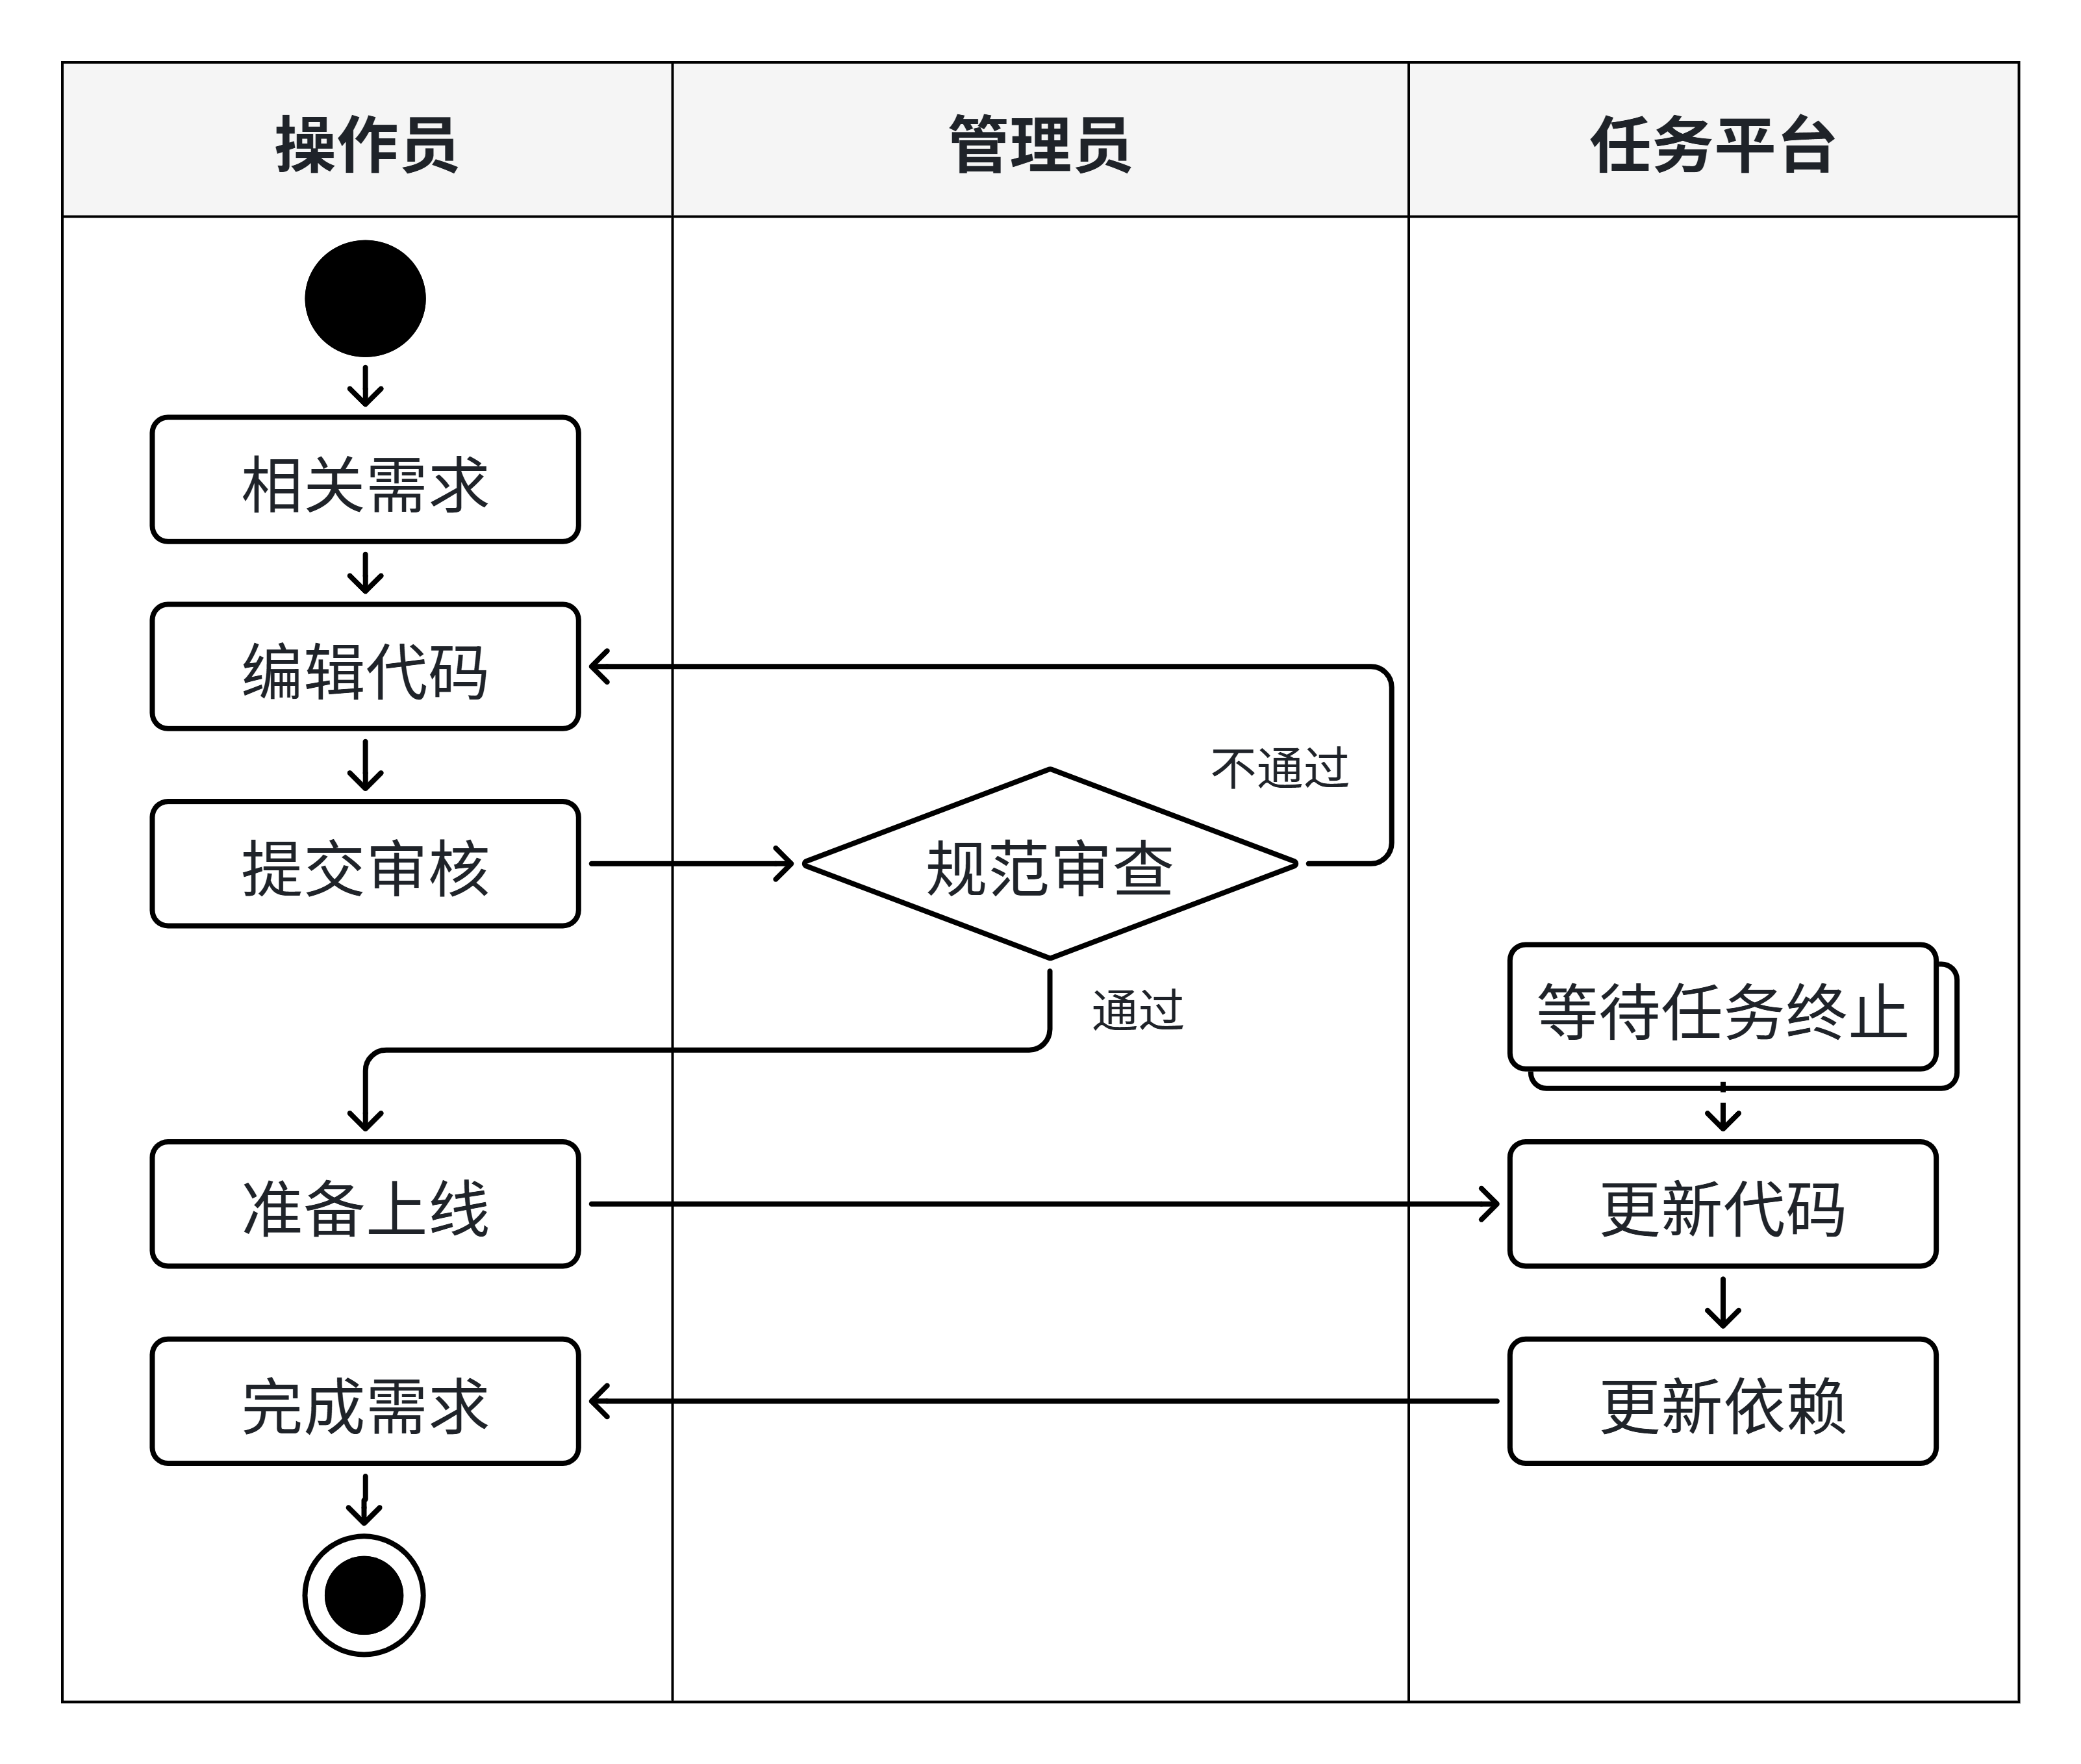
\includegraphics[width=\linewidth]{figures/5/任务编辑垂直泳道图.png}
    \caption{任务编辑泳道图}
    \label{fig:enter-label}
\end{figure}

\subsection{异常捕获机制}

本层异常捕获机制的设计，主要是为配合上文任务调度层中的容错与恢复机制而使用，旨在通过及时捕获并处理异常，为调度层的容错策略提供支持，确保系统在出现问题时能够高效执行恢复操作，提升整体运行的稳定性。任务调度层“容错与恢复机制”的核心功能是对本层抛出的异常进行判断、分析与恢复，故本层的主要职责则是精准抛出异常，并附带完整的调试与纠错信息，为上层的准确判断提供依据。这种分层协作机制，通过明确的功能划分，确保异常从捕获到处理的全流程高效衔接 —— 本层负责 “精准输出问题”，上层专注 “高效解决问题”，二者形成闭环，有效提升了系统应对故障的响应速度与处理精度。

从实际运行来看，本层抛出的异常信息越详尽，任务调度层的恢复策略就越具针对性。例如，当检测到资源占用超限的异常时，本层会同步上传资源使用曲线、进程 ID 等关键数据，调度层便能据此快速定位冲突进程，而非盲目重启系统，这也体现了分层设计在系统稳定性保障中的关键价值。由于不同任务需要向系统提交的异常信息存在差异，因此本机制处于持续开发迭代的状态。操作员在部署新的任务代码前，可向系统开发者提出需求，要求监测额外信息；开发者接到需求后，会对系统进行改进，以满足操作员对任务监控信息的需求。一般而言，新增一个监控指标的工作量相对有限，相应的迭代开发周期约为半天，因此不会对任务交付进度造成显著影响。本系统任务执行模块异常处理流转状态机如图5.12所示。

\begin{figure}[htbp]
    \centering
    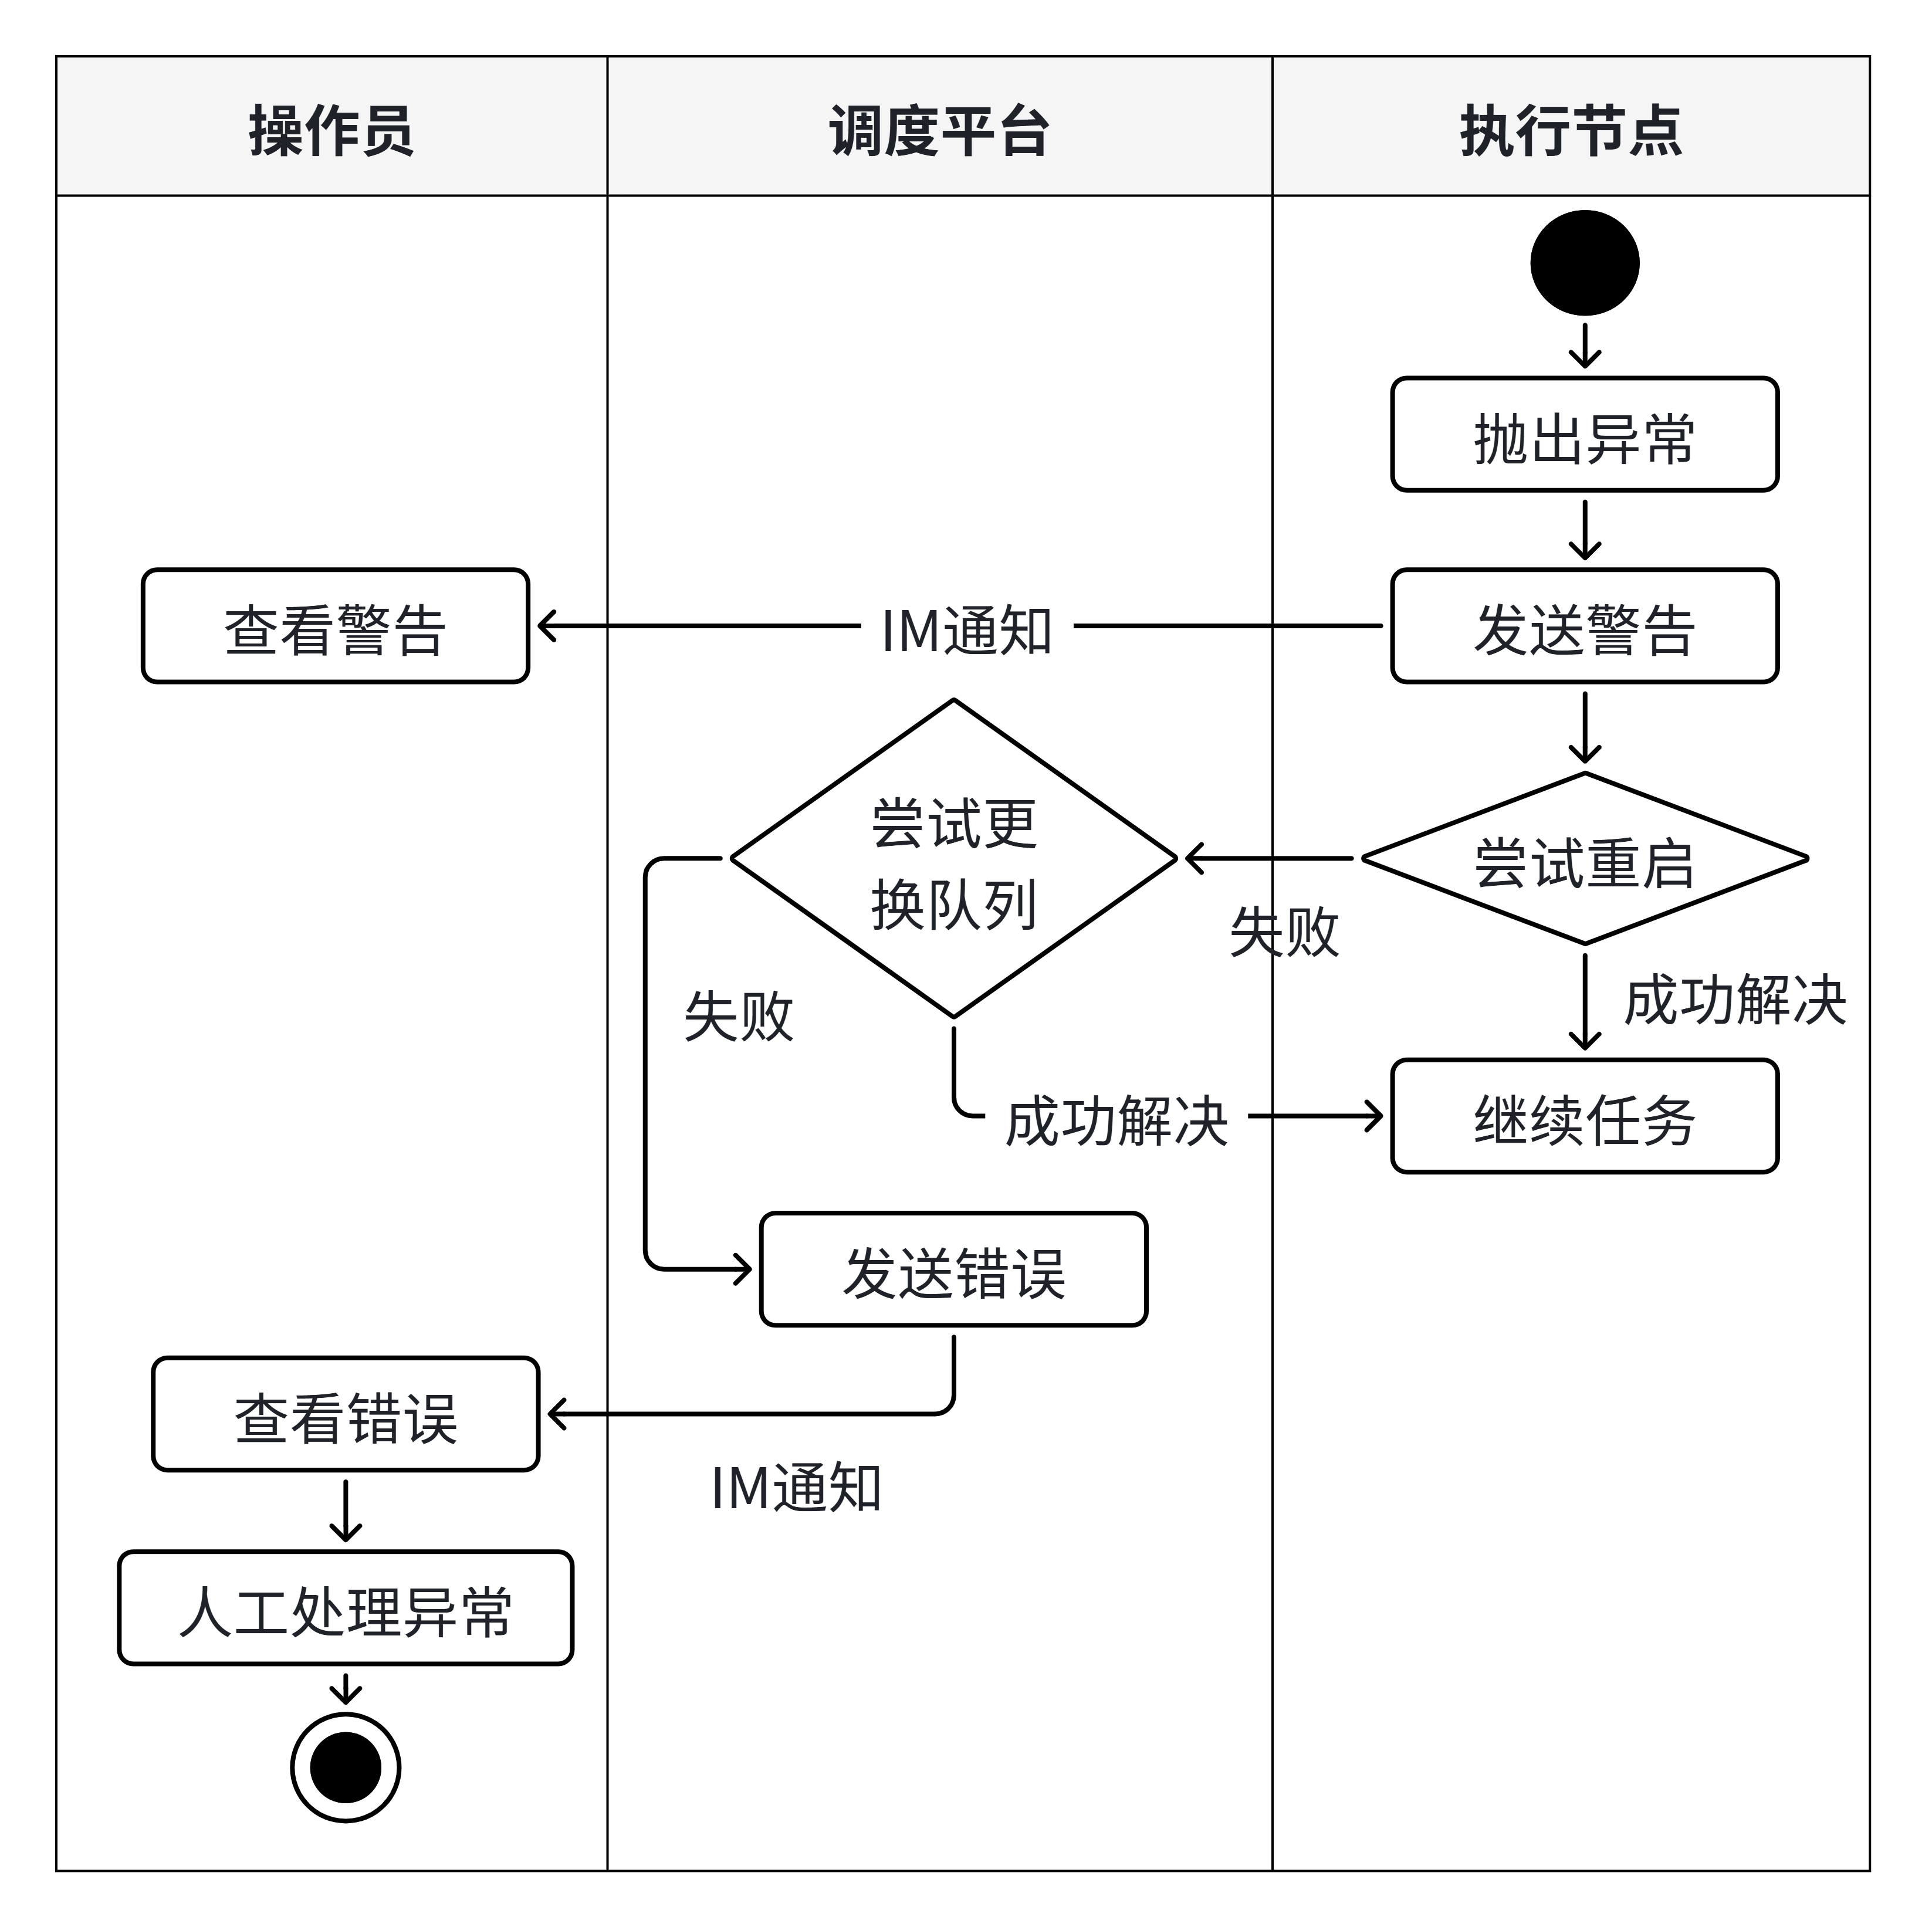
\includegraphics[width=\linewidth]{figures/5/异常处理状态流转.png}
    \caption{异常处理状态流转泳道图}
    \label{fig:enter-label}
\end{figure}

\section{系统总体工作流程}

流程从操作员开始。操作员通过网页操作并填入参数，向调度平台Web端发送请求。调度平台Web端接收到请求后，进行HTTP 请求处理。随后，请求进入调度平台服务器。在调度平台服务器内，请求处理过程分为多个步骤。首先是鉴权请求，确保请求来源的合法性和安全性。接着进行初步处理，对请求进行初步分析和准备。然后是调度算法，通过预设的算法逻辑，确定任务的优先级、资源分配和执行顺序等关键因素。调度算法完成后，进行任务路由，即将任务分配到合适的执行队列中。最后，任务执行队列负责执行任务，确保任务按照预定的计划和要求顺利完成。

\section{本章小结}

本章围绕AI调度三大问题展开详细设计与实现。针对AI特性适配不佳、操作复杂的问题，API接入层通过权限鉴定模块和数据校验模块简化操作、提升适配性；针对无法判断任务执行条件、依赖人工的问题，任务调度层设计任务可用性检测机制与状态机，结合数据同步模块实现任务自动调度；针对无法识别资源互斥的问题，通过资源可用性检测与负载均衡算法优化资源分配，搭配容错恢复与异常捕获机制保障稳定。同时任务执行层明确参数传递与代码管理流程，整体构建起覆盖API、调度、执行的系统架构。

\makeatletter
\@openrightfalse
\makeatother
\chapter{系统测试与分析}

本章旨在通过严谨的实验设计与多维度的性能评估，对本文提出的面向AI多任务场景的资源调度系统进行全面系统性的验证。实验依托腾讯TEG真实业务场景构建测试基准，重点围绕API接入层的适配鲁棒性、任务调度层的决策自动化程度以及任务执行层的资源互斥治理效能展开。通过对系统各功能模块及非功能性指标的深度压测，本章不仅验证了分层解耦架构在解决异构数据纠偏与算力冲突难题中的有效性，更进一步论证了系统在提升大规模AI任务并发周转率及优化算力资源周转效能方面的显著优势，为后续系统的工业级应用与迭代优化提供了详实的数据支撑。

\section{测试概述}

\subsection{开发与测试环境}

本系统的开发环境构建于高性能硬件基础之上，采用 Intel Core i9-13900K 处理器配合 64GB DDR5 高速内存，以满足调度系统在多容器并发运行及复杂逻辑编译时的算力需求。特别地，配置 NVIDIA GeForce RTX 4090 (24GB 显存) 显卡，旨在为 AI 大模型任务的参数画像识别与本地逻辑调试提供必要的算力支撑。软件层面，系统以 Debian 为核心开发系统，利用 Python 3.10 实现 API 接入层的数据纠偏与调度算法的核心逻辑。通过 Docker 容器化技术，实现了开发环境与运行环境的高度隔离，确保了异构数据映射机制在不同计算节点间的可移植性与一致性。本系统的开发环境如表6.1所示。

\begin{table}[htbp]
\centering
\caption{系统开发环境表}
\begin{tabularx}{\textwidth}{llXl}
\toprule
\textbf{环境类别} & \textbf{配置项目} & \textbf{详细规格} & \textbf{主要用途} \\
\midrule
硬件资源 & CPU & Intel Core i9-13900K @ 3.0GHz & 逻辑编译与计算 \\
硬件资源 & 内存 & 64GB DDR5 5600MHz & 多容器并行运行 \\
硬件资源 & GPU & NVIDIA GeForce RTX 4090 & 本地 AI 模型调试 \\
操作系统 & 开发系统 & Debian & 核心开发环境 \\
编程语言 & Python & Version 3.10 & 核心后端逻辑实现 \\
开发工具 & IDE & VS Code & 代码编写与断点调试 \\
容器化 & Docker & Version 24.0.5 & 开发环境隔离与镜像构建 \\
\bottomrule
\end{tabularx}
\end{table}

为深度验证系统在 AI 多任务场景下的调度性能与资源隔离能力，本研究搭建了一套基于 Kubernetes (Tencent TKE) 的分布式集群测试环境，由 1 台主节点与 2 台工作节点组成，模拟真实工业生产中的分布式计算场景。测试流程利用 Postman 对 API 接入层的鉴权与纠错功能进行全量覆盖验证，并借助 Hey 高性能压测工具模拟高并发任务请求，以此评估系统在极限负载下的吞吐量（RPS）与任务调度延迟。此外，环境涵盖了 CentOS、Debian 及 Windows Server 等异构操作系统，重点验证系统对不同计算底座的兼容性适配。所有测试数据通过 Grafana 进行可视化监控与分析，确保资源互斥智能算法在处理高价值算力冲突时的稳定性和鲁棒性，最终通过 腾讯智研 CI/CD 平台实现研发效能的全流程自动化验证。系统测试与验证环境如表6.2所示。

\begin{table}[htbp]
\centering
\caption{系统测试与验证环境表}
\begin{tabularx}{\textwidth}{llXl}
\toprule
\textbf{测试维度} & \textbf{测试项} & \textbf{环境配置/测试工具} & \textbf{测试目标} \\
\midrule
集群模拟 & 节点数量 & 3台分布式计算节点 (Master*1, Worker*2) & 验证分布式调度能力 \\
编排系统 & Kubernetes & Version 1.28.0 (Tencent TKE 托管版) & 资源动态扩缩容测试 \\
接口测试 & API 调试 & Postman & 后端接口功能验证 \\
性能压测 & 并发测试 & Hey (Golang 编写) & 评估系统吞吐量 (RPS) \\
可视化 & 面板展示 & Grafana & 生成稳定性压力测试报表 \\
兼容性 & 操作系统 & CentOS 7.9, Debian 11, Windows Server & 验证异构环境适配性 \\
自动化测试 & CI/CD 流程 & 腾讯智研 & 验证代码迭代自动化测试 \\
\bottomrule
\end{tabularx}
\end{table}

\subsection{测试方法}

本研究构建了多维度、全链路的测试体系，旨在验证系统在解决 AI 特性适配性、调度决策自动化以及计算资源互斥处理三大核心问题上的有效性。测试工作主要分为功能性测试与非功能性测试。

功能性测试通过开发自测（Unit Testing）与QA团队全案测试相结合，重点校验以下三个层面的逻辑正确性：AI适配与数据纠偏测试利用Postman构造包含全角字符、冗余符号、类型偏差的异构参数报文，验证API接入层在大模型任务参数画像约束下的自动纠正能力，确保下行至执行层的数据纯净度；决策引擎与可用性检测验证模拟不同系统负载水位与运营策略变化，验证调度层逻辑引擎是否能自主判定任务准入状态，消除对人工干预的依赖；资源互斥与并发调度验证通过构造多组竞争同一GPU编号的互斥任务流，验证系统是否能精准识别资源依赖拓扑，在保障临界资源不冲突的前提下，实现由串行向安全并发的转变。

非功能性测试侧重于系统在生产环境（腾讯TEG业务场景）下的工业级表现：性能压力测试采用基于Golang的Hey工具模拟高频并发请求，评估系统在多任务注入时的响应延迟与吞吐量（RPS），确保调度算法在毫秒级内完成决策；稳定性与容错测试依托公司基础设施进行7x24小时长周期运行监测，模拟节点宕机、网络抖动及内存受限（OOM）等异常场景，验证任务状态机的自愈能力与资源自动释放机制。异构兼容性测试在TKE托管的异构计算集群中，验证系统对CentOS、Debian及Windows Server等操作系统的适配性，确保参数传递机制在分布式节点间的一致性。

系统采用敏捷迭代模式，通过TAPD平台实现缺陷的生命周期管理。开发人员完成初测后，由QA团队进行全方位的回归测试。程序上线后，通过自动化监控系统捕获实时性能指标，并设立操作员反馈渠道，针对实际运行中出现的特殊AI算子适配需求或性能瓶颈进行持续优化与策略更新。

\section{功能测试}

功能测试部分通过对API接入层、任务调度层及任务执行层的全方位测试，系统性验证了本文所设计的资源调度系统在应对AI多任务复杂需求时的有效性。测试过程紧扣本文研究重点，重点针对异构数据适配、调度决策自动化及算力资源互斥治理三大核心问题进行了闭环验证：在API接入层测试中，验证了基于参数画像的自动化纠偏逻辑对AI任务异构数据的鲁棒性支持；在任务调度层测试中，证实了环境感知驱动的逻辑引擎能够准确判定任务可执行性，实现了调度流程的去人工化；在任务执行层与资源管理测试中，验证了资源互斥智能分析算法对GPU等独占性资源的高效管控，解决了因资源抢占导致的任务串行瓶颈。实验数据表明，系统各项核心指标均达到预期设计要求，功能用例通过率为100\%，为实现AI多任务的高效并发调度提供了坚实的技术保障。

\subsection{API接入层测试}

本次 API 功能接入层测试围绕权限鉴定与数据校验两大模块展开，模拟多场景验证功能准确性，所有案例结果均符合预期。权限鉴定模块中，组内用户登录可顺利完成身份验证，组外用户登录被拒绝；组内用户登录后能成功发起任务，组外用户无论是否登录，发起任务均被阻断并提示无权限，有效划分权限边界；数据校验模块里，提交合法数据可正常流转至业务模块；提交语法错误数据（如分隔符、引号问题），接入层会自动更正后继续处理；提交类型错误数据（如年龄字段为字符串、日期格式不符），则会阻断任务并通知操作员，避免错误数据影响下游业务。
API接入层数据校验与自动纠正功能测试用例如表6.3所示。

\begin{table}[htbp]
\centering
\caption{API接入层数据校验与自动纠正功能测试表}
\begin{tabularx}{\textwidth}{lXll}
\toprule
\textbf{需求项} & \textbf{预期结果} & \textbf{实际结果} & \textbf{测试状态} \\
\midrule
AI参数画像匹配 & 成功匹配Prompt/超参数Schema，系统判定为合法通过 & 100\%符合预期 & 通过 \\
异构类型校验   & 基于Pydantic实施类型检查，确保异构数据类型合法通过 & 100\%符合预期 & 通过 \\
全角标点纠偏   & 系统自动将全角符号转化为半角标点，实现修正通过 & 100\%符合预期 & 通过 \\
冗余符号清理   & 自动剔除输入中的冗余括号、空格等，实现修正通过 & 100\%符合预期 & 通过 \\
数值类型推断   & 实现浮点数向整数的无损转化，确保数据修正通过 & 100\%符合预期 & 通过 \\
字符串格式化   & 成功去除字符串首尾空格及不可见字符，实现修正通过 & 100\%符合预期 & 通过 \\
日期格式统合   & 各种日期字符串统一格式化为“YYYY-MM-DD”并修正通过 & 100\%符合预期 & 通过 \\
校验结果反馈   & 系统完整汇总校验报告并成功向调度平台下发提示 & 100\%符合预期 & 通过 \\
\bottomrule
\end{tabularx}
\label{tab:api_access_test}
\end{table}

此外，本工作还对权限鉴定、任务管理及脚本审核等核心基础功能进行了全面验证。权限鉴定测试结果显示组内与组外用户的拦截逻辑均100\%符合预期；任务管理测试结果显示本系统实现了任务表单的准确入库与状态机逻辑的正常流转；脚本审核功能验证了系统对AI执行逻辑安全性的严密管控，确保未获审批的脚本禁止执行。测试项的全部通过，标志着API接入层在安全准入与基础治理维度已具备支撑大规模异构AI任务高效流转的工业级可靠性。
API接入层其余测试用例表如表6.4所示。

\begin{table}[htbp]
\centering
\caption{API接入层其余功能测试表}
\begin{tabularx}{\textwidth}{lXll}
\toprule
\textbf{需求项} & \textbf{预期结果} & \textbf{实际结果} & \textbf{测试状态} \\
\midrule
权限鉴定 & 组内用户通过，组外用户拦截并提示无权限 & 100\%符合预期 & 通过 \\
任务管理 & 任务表单正确写入数据库，状态流转正常 & 100\%符合预期 & 通过 \\
脚本审核 & 审核通过后脚本上线，未审核脚本禁止执行 & 100\%符合预期 & 通过 \\
\bottomrule
\end{tabularx}
\end{table}

\subsection{任务调度层测试}

任务调度层测试聚焦任务可用性、资源可用性、容错与恢复三大核心维度，通过模拟不同业务场景验证调度功能的准确性与稳定性，所有测试案例执行结果均符合预期。

任务可用性测试中，对于过期任务，调度层能精准识别其时间属性并判定超出执行范围，不予调度；对于普通有效任务，调度层则按预设规则完成解析、优先级排序与指令下发，确保正确调度，从而保障任务执行的时间有效性。针对决策依赖难题，本测试验证了“场景策略注入”功能，模拟节假日或运维封网时，系统根据动态加载的JSON策略文件，自动调整任务准入优先级，展现了极高的灵活性与策略一致性。测试进一步验证了负载回落后的系统表现。当环境指标降至安全区间后，被挂起的任务能自动被调度器唤醒并重新入队执行，全程无需人工重启指令，实现了调度流程的闭环管理。任务可用性检测功能的 8 项核心用例通过率均为 100\%。实验数据论证了逻辑引擎在处理复杂环境约束时的鲁棒性，证实了系统已成功由“人工经验驱动”转型为基于实时状态感知的“智能自动化调度”，大幅降低了运维人力投入。任务可用性检测功能测试表如表 6.5 所示。

\begin{table}[htbp]
\centering
\caption{任务可用性检测功能测试表}
\begin{tabularx}{\textwidth}{lXll}
\toprule
\textbf{需求项} & \textbf{预期结果} & \textbf{实际结果} & \textbf{测试状态} \\
\midrule
系统负载检测 & 系统能够实时采集各项负载指标，并准确输出当前负载状态值 & 100\%符合预期 & 通过 \\
负载阈值配置 & 管理员可成功设置自定义负载阈值，系统保存后配置立即生效 & 100\%符合预期 & 通过 \\
任务启动判断 & 系统通过对比当前负载与预设阈值，准确作出允许或禁止启动的决策 & 100\%符合预期 & 通过 \\
高负载任务限制 & 当系统处于过载状态时，能有效拦截高耗能任务并弹出相应提示 & 100\%符合预期 & 通过 \\
配置修改记录 & 系统能完整记录管理员的配置修改操作，并成功生成审计日志 & 100\%符合预期 & 通过 \\
异常场景触发 & 在节假日等预设异常场景下，系统能自动激活相应的任务限制规则 & 100\%符合预期 & 通过 \\
任务拦截反馈 & 任务因过载被拦截后，系统能清晰向用户告知“负载过高”的具体原因 & 100\%符合预期 & 通过 \\
负载回落恢复 & 当实时负载回落至阈值以下时，系统能自动恢复任务的正常启动功能 & 100\%符合预期 & 通过 \\
\bottomrule
\end{tabularx}
\label{tab:task_scheduling_test}
\end{table}

针对人工智能多任务场景下的算力冲突痛点，资源可用性测试紧密围绕任务需求与底层计算资源的匹配关系展开。系统首先依托资源提前注册与任务资源声明功能，要求任务在提交阶段即标注具体的临界资源需求，从而确保算力元数据能够准确入库并建立稳固的任务关联。在核心的调度决策阶段，调度层深度利用任务互斥判定机制，对在途任务的临界资源需求进行实时对比分析。若判定目标资源处于空闲状态，则通过执行权限判断模块立即下发启动指令；而一旦检测到资源占用冲突，系统则会自动拦截任务下发并向操作员反馈清晰的互斥冲突提示，同时将该任务平滑地加入高可靠的资源等待队列中。此外，调度层内置的资源释放监测模块会全时段实时跟踪算力资源的动态占用变化。一旦捕捉到资源由锁定转为空闲的瞬时状态，系统便会立即触发等待任务唤醒机制，驱动执行队列进行自动调度与分发，从而有效缩短任务间的间隙空耗。在容错与恢复测试维度，系统通过模拟计算节点关机或断电等极端硬件故障场景，充分验证了调度层能凭借心跳检测技术敏锐识别节点的离线状态。系统随后会迅速触发预设的故障转移机制，将尚未完成的算力任务重新分配至集群内的其他可用节点执行，从底层有效保障了AI业务的连续性与系统运行的稳健性。本项资源可用性检测的具体功能测试用例与验证结果详见表6.6。

\begin{table}[htbp]
\centering
\caption{资源可用性检测功能测试表}
\begin{tabularx}{\textwidth}{lXll}
\toprule
\textbf{需求项} & \textbf{预期结果} & \textbf{实际结果} & \textbf{测试状态} \\
\midrule
资源提前注册 & 任务能够声明所需资源并完成登记，确保资源信息成功入库 & 100\%符合预期 & 通过 \\
任务资源声明 & 任务提交时可标注具体资源需求，系统成功记录任务与资源的关联关系 & 100\%符合预期 & 通过 \\
任务互斥判定 & 系统对比任务所需的临界资源，能够准确识别并标记存在互斥关系的任务 & 100\%符合预期 & 通过 \\
执行权限判断 & 检查目标资源的占用状态，并根据检测结果准确作出允许或拒绝执行的决策 & 100\%符合预期 & 通过 \\
任务等待入队 & 在无可用资源时自动标记任务状态，并将其平滑加入资源等待队列中 & 100\%符合预期 & 通过 \\
资源释放监测 & 实时跟踪并捕捉资源占用的动态变化，确保能够及时识别资源的空闲状态 & 100\%符合预期 & 通过 \\
等待任务唤醒 & 当资源释放并处于空闲状态时，成功触发队列调度并唤醒等待中的任务 & 100\%符合预期 & 通过 \\
互斥冲突提示 & 当发生任务互斥导致无法执行时，系统能清晰向用户提示资源占用原因 & 100\%符合预期 & 通过 \\
\bottomrule
\end{tabularx}
\label{tab:resource_availability_test}
\end{table}

针对任务调度层除了可用性检测以外的其他关键职能，本测试汇总了负载均衡、数据同步以及容错恢复维度的测试验证结果，这些测试项旨在验证系统在分布式异构环境下保障执行效能与运行韧性的能力，深度契合了第三章中提出的各项非核心功能需求。

在负载均衡与性能优化方面，测试重点针对任务执行节点在物理基础与运行环境上的显著异构性展开。测试证实，调度层通过引入智能权重分配算法，能精准采集各节点的实时负载指标并动态分析AI任务的资源亲和性特征，将计算密集型推理任务优先指派至算力充裕的GPU节点，从而在多任务高并发场景下维持高吞吐与低延迟的稳健运行状态。在数据同步维度，本系统构建了高可靠、强一致的同步机制以规避子模块间因信息流转失真导致的任务逻辑偏离。测试验证了基于高性能中间件的消息同步底座是否能实现数据的透明流转，确保API接入层预先完成的参数纠偏与类型推断结果能实时、完整地透传至任务执行节点，从而为算力的精准调度提供坚实的数据基础。在容错与恢复能力验证中，考虑到AI任务具备执行周期长且算力消耗高的特征，系统必须具备对非致命性异常的动态识别与自助修复能力。实验重点模拟了网络通信韧性、磁盘空间不足、以及因异构环境导致的参数类型冲突等典型异常场景，验证了系统是否能依据指数退避机制执行自动重试，并利用智能纠偏规则对float与int类型冲突进行实时修复。测试结果显示，系统在遭遇计算节点宕机或网络抖动时，能迅速通过状态机重置触发故障转移机制，将任务重新分配至可用节点恢复执行，成功实现了由人工排障向引擎自愈的深度转型，各项指标均100\%符合预期。任务调度层其余功能测试表如表6.7所示。

\begin{table}[htbp]
\centering
\caption{任务调度层其余功能测试表}
\begin{tabularx}{\textwidth}{lXll}
\toprule
\textbf{需求项} & \textbf{预期结果} & \textbf{实际结果} & \textbf{测试状态} \\
\midrule
负载均衡 & 任务按权重比例分发至异构执行节点 & 100\%符合预期 & 通过 \\
数据同步 & 任务池状态与执行队列实时保持一致 & 100\%符合预期 & 通过 \\
容错恢复 & 任务重新入队并在可用节点恢复执行 & 100\%符合预期 & 通过 \\
\bottomrule
\end{tabularx}
\end{table}

\subsection{任务执行层测试}

任务执行层作为算力调度的最终落地单元，其测试核心在于验证分布式环境下参数传递的准确性、任务动态编辑的即时性以及异常捕获机制的鲁棒性。本测试旨在确保调度中枢下发的逻辑指令能精准转化为底层的算力输出，并验证系统在极端执行工况下的自愈与反馈能力。

为了验证系统是否有效解决AI特性适配不佳及异构数据处理能力不足的痛点，本研究对参数传递环节进行了全方位的覆盖测试。系统通过“参数封装处理”与“传输校验机制”，确保了异构参数在分布式节点间流转时的完整性系统内置了“任务丢失检测”与“断点续传支持”，测试结果表明，系统在发现传输中断后能准确触发重试逻辑，并支持大参数的分片传输，有效避免了因网络异常导致的算力资源空耗。系统重点验证了“远程附件拉取”与“参数路径替换”功能。实验通过构造包含多组对象存储（COS）链接的报文，证实执行层能自动化完成远程素材的并发下载，并将参数中的远程URL动态重定向为本地物理路径。这充分论证了本文设计的参数传递协议与环境自愈逻辑具备极高的鲁棒性，为后续实现复杂的自动化决策与资源精细化治理提供了坚实的数据闭环保障。参数传递功能测试表如表6.8所示。

\begin{table}[htbp]
\centering
\caption{参数传递功能测试表}
\begin{tabularx}{\textwidth}{lXll}
\toprule
\textbf{需求项} & \textbf{预期结果} & \textbf{实际结果} & \textbf{测试状态} \\
\midrule
参数封装处理 & 能够打包任意类型参数并成功生成传输数据包  & 100\%符合预期 & 通过 \\
透明传输处理 & 成功屏蔽网络传输细节并实现无感调用  & 100\%符合预期 & 通过 \\
传输校验机制 & 准确验证参数完整性并确保数据准确  & 100\%符合预期 & 通过 \\
任务丢失检测 & 实时监控传输状态并在发现丢失时触发重试  & 100\%符合预期 & 通过 \\
远程附件拉取 & 成功下载远程附件至本地并生成本地文件路径  & 100\%符合预期 & 通过 \\
参数路径替换 & 将远程路径改为本地路径以适配本地执行环境  & 100\%符合预期 & 通过 \\
断点续传支持 & 实现大参数分片传输并支持中断后继续  & 100\%符合预期 & 通过 \\
传输结果反馈 & 准确返回参数处理状态并告知成功或失败原因  & 100\%符合预期 & 通过 \\
\bottomrule
\end{tabularx}
\end{table}

本测试证实了执行层在AI多任务管理中的灵活性与可靠性。系统能精准执行撤销指令并终止无效进程，通过即时释放GPU等独占资源规避算力空耗。此外，系统支持异构参数编辑，并能驱动新实例重新联动决策引擎与互斥分析逻辑。100\%的操作反馈准确率保障了任务全生命周期的观测透明度，相关数据见表6.9。

\begin{table}[htbp]
\centering
\caption{任务编辑功能测试表}
\begin{tabularx}{\textwidth}{lXll}
\toprule
\textbf{需求项} & \textbf{预期结果} & \textbf{实际结果} & \textbf{测试状态} \\
\midrule
任务撤销触发 & 能够正确接收撤销指令并启动任务终止流程 & 100\%符合预期 & 通过  \\
任务参数修改 & 成功完成任务参数及类型的编辑并保存修改内容 & 100\%符合预期 & 通过  \\
任务重启执行 & 在符合条件时成功启动新任务并进入运行态 & 100\%符合预期 & 通过  \\
操作结果反馈 & 准确返回撤销或重启状态并告知成功或失败原因 & 100\%符合预期 & 通过  \\
\bottomrule
\end{tabularx}
\end{table}

本工作针对人工智能大模型调度场景下任务高算力消耗且周期长的特征，对系统全链路的风险识别与自愈能力进行了严谨验证。测试结果证实，系统能够实时细致地监测CPU、内存及文件描述符等关键指标，并基于历史数据准确触发预警通知，从而在感知识别维度保障了运行环境的稳定性。在拦截与保护层面，异常任务暂停与数据暂存功能的通过，确保了系统能在终止风险任务的同时保存中间计算成果，从底层化解了因非预期中断导致的算力空耗难题。此外，依托Python异常处理流程实现的自动化日志捕获、信息即时上报及原因深度分析，显著提升了运维反馈的精确度，配合100\%符合预期的系统恢复尝试逻辑，标志着系统已成功实现从“人工排障”向“引擎自愈”的智能化转型。全体测试项的顺利通过，充分论证了执行层在复杂异构工况下具备极高的鲁棒性，为支撑大规模AI任务的高效并发周转构筑了稳固的安全防线。异常捕获功能测试表如表6.10所示。

\begin{table}[htbp]
\centering
\caption{异常捕获功能测试表}
\begin{tabularx}{\textwidth}{lXll}
\toprule
\textbf{需求项} & \textbf{预期结果} & \textbf{实际结果} & \textbf{测试状态} \\
\midrule
系统指标监测 & 能够实时、细致地监测CPU、内存及文件描述符等关键指标并输出数据 & 100\%符合预期 & 通过  \\
异常预测预警 & 基于历史数据准确识别指标异常，并成功向相关人员触发预警通知 & 100\%符合预期 & 通过  \\
异常任务暂停 & 发现系统风险时能够即刻终止目标任务，避免不必要的资源浪费 & 100\%符合预期 & 通过  \\
任务数据暂存 & 在异常任务暂停或终止前，成功保存中间数据以防止工作量丢失 & 100\%符合预期 & 通过  \\
异常捕获 & 依托Python异常处理流程，成功采集任务运行时产生的完整异常日志 & 100\%符合预期 & 通过  \\
异常信息上报 & 将详尽的异常详情及日志信息即时推送至相关人员以通知故障处理 & 100\%符合预期 & 通过  \\
异常原因分析 & 自动整理并提供Traceback日志及数据报表，为故障排查提供分析依据 & 100\%符合预期 & 通过  \\
系统恢复尝试 & 能够通过重启服务、释放被占用的临界资源等手段恢复系统正常运行 & 100\%符合预期 & 通过  \\
\bottomrule
\end{tabularx}
\end{table}

\section{非功能测试}

\subsection{性能测试}

性能测试不仅是验证系统基础吞吐能力的手段，更是评估资源互斥智能分析与调度决策逻辑在极端环境下效能的关键环节。其核心意义在于通过高并发压力模拟，验证系统是否真正具备实时处理能力，从而确保系统能彻底消除传统串行调度模式引发的瓶颈，支撑AI算力资源的高效并发周转。性能测试的重点在于验证“资源互斥智能分析”与“自动化决策引擎”的响应延迟是否控制在极低阈值内。通过在高并发环境下实时采集调度指令的下发耗时，本测试能够论证系统在保障临界资源不冲突的前提下，实现由“保守串行”向“安全并发”转型的实际效能，进而为计算集群利用率的提升提供数据支撑。

为了精准匹配AI高频研发场景下对“无感官卡顿”的严苛需求，本测试选用了基于 Golang编写的高性能压测工具Hey。由于Golang在并发处理与运行性能上相较于Python具备显著优势\cite{wang2023}，能够更客观、高效地对系统后端实施极限压测，从而准确捕捉大规模附件流转及批量指令控制时的响应延迟。测试结果表明，系统在多任务注入场景下依然保持了毫秒级的调度响应速度，证实了其在处理AI异构任务时具备极高的鲁棒性与高吞吐处理能力，完全符合预期的性能目标。具体的性能数据如表6.11所示。

\begin{table}[htbp]
\centering
\caption{性能测试结果表}
\begin{tabular}{lll}
\toprule
测试内容 & 预期结果 & 实际结果 \\
\midrule
10 并发下提交任务平均响应时间 & 响应时间 < 50 ms & 平均 14 ms \\
10 并发下删除任务平均响应时间 & 响应时间 < 50 ms & 平均 11 ms \\
10 并发下编辑任务平均响应时间 & 响应时间 < 50 ms & 平均 13 ms \\
100 并发下提交任务平均响应时间 & 响应时间 < 100 ms & 平均 32 ms \\
100 并发下删除任务平均响应时间 & 响应时间 < 100 ms & 平均 28 ms \\
100 并发下编辑任务平均响应时间 & 响应时间 < 100 ms & 平均 30 ms \\
1000 并发下提交任务平均响应时间 & 响应时间 < 500 ms & 平均 168 ms \\
1000 并发下删除任务平均响应时间 & 响应时间 < 500 ms & 平均 145 ms \\
1000 并发下编辑任务平均响应时间 & 响应时间 < 500 ms & 平均 152 ms \\
\bottomrule
\end{tabular}
\label{tab:perf_concurrent}
\end{table}

\subsection{稳定性测试}

本工作通过对关机重启、断电、网络中断、多任务并发及磁盘异常等复杂工况的模拟，全面验证了系统在工业级生产环境下的长期运行可靠性与自动化修复能力。针对AI任务执行周期长且算力成本高的特征，测试证实系统在遭遇硬件故障或网络抖动时，能够依托环境感知的自愈机制实现程序的自动重连与未完成任务的断点续传，确保了数据完整性并有效规避了算力空耗。同时，多任务并发执行的成功校验进一步论证了资源互斥智能分析算法在处理高价值算力冲突时的精确度，保障了在共享资源环境下各任务结果的正确性。此外，系统在磁盘空间不足等极限场景下的安全停止与预警反馈，配合100\%符合预期的测试结果，标志着本研究已成功构建起覆盖全生命周期的稳健运行防线，从技术底层实现了调度决策的去人工化与业务连续性保障 。稳定性测试用例如表6.12所示。

\begin{table}[htbp]
\centering
\caption{稳定性测试用例表}
\begin{tabular}{lll}
\toprule
测试内容 & 预期结果 & 实际结果 \\
\midrule
关机重启 & 程序自动恢复，数据无丢失 &  100\%符合预期 \\
断电 & 继续未完成任务 &  100\%符合预期 \\
网络中断 & 程序重连网络，任务继续 &  100\%符合预期 \\
多任务并发执行 & 任务无冲突，结果正确 &  100\%符合预期 \\
磁盘空间不足时 & 提示空间不足，程序停止 &  100\%符合预期 \\
\bottomrule
\end{tabular}
\label{tab:my_label}
\end{table}

\subsection{兼容性测试}

兼容性测试旨在验证系统对多元化AI任务范式与多态运行环境的深度适配能力。测试重点评估了系统在异构计算集群中的鲁棒性，从根源上解决了子问题一中AI特性适配欠佳的难题。本工作针对AI任务强数据依赖的特征，测试了多类操作系统环境。验证证实，参数传递机制与远程附件拉取逻辑在跨集群分配策略下表现一致，确保了异构计算底座上的逻辑一致性与数据鲁棒性。系统在不同指令集架构与操作系统组合下均能稳定运行且无报错。测试结果表明，本文的设计能够应对环境偏差导致的适配风险，为系统的工业级推广提供了坚实的兼容性保障。验证结果如表6.13所示。

\begin {table}[htbp]
\centering
\caption {任务执行层兼容性测试用例表}
\begin {tabular}{lll}
\toprule
测试内容 & 预期结果 & 实际结果 \\
\midrule
Linux系统x86服务器 & 程序适配架构，运行稳定无报错 &  100\%符合预期 \\
Linux系统ARM服务器 & 程序适配架构，运行稳定无报错 &  100\%符合预期 \\
Windows系统x86服务器 & 程序适配架构，运行稳定无报错 &  100\%符合预期 \\
Windows系统ARM服务器 & 程序适配架构，运行稳定无报错 &  100\%符合预期 \\
\bottomrule
\end {tabular}
\label {tab:my_label}
\end {table}

\section{本章小结}

本章对面向AI多任务场景的资源调度系统进行了系统性的测试验证与结果分析。通过模拟真实的生产业务环境，从功能完备性、性能高效性、系统稳定性及环境兼容性四个维度开展了全方位评估。通过对异构数据纠偏、自动化准入决策及临界资源互斥识别等关键模块的验证，证实了本系统能有效解决AI任务参数复杂、调度依赖人工及计算资源冲突等行业痛点。

\makeatletter
\@openrightfalse
\makeatother
\chapter{结论与展望}

\section{结论}

作为一项前沿应用技术，人工智能大模型已广泛融入众多领域，为人们的生产生活带来极大便利。随着人工智能大模型的迅猛发展，各技术公司面临的相关开发测试任务日益繁重。为顺应AI发展的实际需求，本论文聚焦于AI多任务调度问题的特性展开深入研究，着力解决现有编排模式与调度系统无法满足AI大模型任务发展需求的难题。在此基础上，本系统精心设计了三个工程层次，并对各层次内部进行了细致规划。具体研究工作与贡献如下：

\begin{enumerate}
\item 攻克了传统调度系统对AI相关特性适配不佳的难题。API 功能接入层与任务执行层紧密围绕人工智能大模型的独特需求展开深度适配。在参数类型方面，充分考虑到 AI 大模型处理数据的多样性和复杂性，对参数进行了精细化设计，确保能够准确传递各种类型的数据，满足不同模型的输入要求。在数据传输方式上，针对 AI 大模型数据量大、实时性要求高的特点，选用了合适的传输协议和策略，减少数据传输延迟和丢包率，实现了数据的快速、稳定传输。通过这些维度的深度适配，使系统在各个环节高度贴合人工智能大模型任务的特性，有力地化解了现有任务调度系统与人工智能大模型任务适配度不理想的困境，为 AI 任务的高效执行奠定了坚实基础。
\item 成功解决了现阶段无法准确判断 AI 任务是否具备执行条件的关键问题。任务调度层创新性地设计了任务可用性检测机制，并将其与先进的调度算法深度融合、协同运作。该机制基于对 AI 任务的详细分析，综合考虑任务的优先级、资源需求、前置条件以及当前系统的资源状态等多方面因素，构建了一套判断体系。借助该机制与算法的协同作用，本系统能够精准洞察 AI 任务是否具备执行条件，避免了因盲目执行任务而导致的资源浪费和效率低下问题。这一举措不仅有效节省了大量的人力成本，还极大地提高了系统的整体运行效率和稳定性，确保了 AI 任务在复杂多变的环境中能够有条不紊地推进。
\item 设计了专门针对 AI 特有资源的资源互斥检测机制，解决了在 AI 多任务场景下难以识别资源互斥的问题。任务调度层不仅设计了资源可用性检测机制，还结合 AI 多任务场景下资源使用的特点，开发了一套针对性的检测算法。该算法能够实时监测各个任务对资源的占用情况，准确识别出 AI 多任务场景下潜在的资源互斥状况。收到任务时，若检测到资源互斥，系统能够迅速做出响应，通过合理调整任务执行顺序或重新分配资源等策略，避免因资源冲突而导致的任务失败或系统性能下降。这一机制的引入显著提高了调度效率，保障了 AI 多任务在共享资源环境下的高效、稳定运行。
\item 顺利完成了对本系统的全面整合测试。测试阶段，采用了多种测试方法和场景模拟，涵盖功能测试、性能测试、稳定性测试等多个维度。经过大量的实际测试和优化，本系统在实际应用中展现出卓越的性能。
\end{enumerate}

\section{展望}

本系统的设计与实现能够满足当前腾讯公司AI任务调度的需求，但AI大模型作为一个新兴领域，目前仍处于发展初期。在可预见的未来，AI大模型将持续快速演进。因此，即便本系统当前能够适配现有需求，仍需紧跟技术发展趋势，不断进行调整与优化，才能在AI技术的迭代浪潮中保持领先优势。本系统需要继续拓展与挖掘的地方如下：

\begin{enumerate}
    \item 适配更多样的临界资源。AI发展的早期，其依赖的临界资源主要是GPU服务器。而发展至今日，AI需求的临界资源早已不局限于硬件资源。以最近热议的MCP为例，有的MCP依赖的资源也是互斥使用的，本系统可以以此为创新点，挖掘与MCP服务对接的可能性。
    \item 完善数据报表功能。当前数据报表的展示格式主要由开发者与系统维护人员沟通实现。日后可以增加AI大模型自动分析任务数据，自动生成报表的功能。在基础数据之上，利用AI智能分析数据报表，既可以节省沟通成本，又可以从不同的视角分析数据。
\end{enumerate}

\makeatletter
\@openrightfalse
\makeatother

\bibliography{bib/ustc}  % 参考文献使用 BibTeX 编译
% \printbibliography       % 参考文献使用 BibLaTeX 编译

\appendix
% \include{chapters/complementary}

\backmatter
\begin{acknowledgements}

岁月的车轮悄然转过，两载有余的硕士研究生生涯即将画上句号。回望这段旅程，从初试录取的欣喜、踏入科大校园的憧憬，到投身企业实习的历练，再到如今论文定稿的如释重负，个中收获不仅体现在学术能力的提升，更在于心智的成长。值此论文完稿之际，谨向所有给予我指导、支持与陪伴的人致以最诚挚的谢意。

首先，衷心感谢我的导师赵功名教授。本论文从选题构思、开题论证到最终定稿，每一步都凝结着赵老师的心血。赵老师严谨治学的态度与敏锐的学术洞察力令我获益匪浅。特别难忘在开题阶段，赵老师通过电话针对论文题目的准确性给予了关键指导，使研究重点得以聚焦；在论文撰写过程中，赵老师更是多次审阅稿件，从逻辑架构到遣词造句均提出了详尽的修改意见，确保了本研究的严密性与规范性。在此，向赵老师表达崇高的敬意。同时，也要感谢张钟高级工程师在项目实践中给予的宝贵建议。

其次，感谢中国科学技术大学软件学院及全体授课教师。学院设置的专业课程体系兼具前沿性与实用性，为我的科研工作打下了坚实的理论基础。同时，感谢学院搭建的实习双选平台，使我有机会进入业界领军企业进行工程实践，在真实场景中提升了解决复杂问题的能力。

感谢我的父母。考研备考至今，父母始终是我最坚强的后盾。正是因为他们在经济上的无私支持与精神上的默默守护，使我能够免于生活琐事的后顾之忧，全身心地投入到学业与研究之中。这份恩情，厚重如山，没齿难忘。

感谢与我并肩作战的同学们。无论是在课程研讨中的思维碰撞，还是在实习期间的相互勉励，大家的陪伴使这段旅程充满了温暖。在论文撰写期间，我们针对学术难题进行的探讨与互助审校，极大地拓宽了我的视野。这段纯粹的同窗情谊是我硕士生涯中最珍贵的财富。

最后，感谢母校中国科学技术大学。“红专并进，理实交融”的校训精神已深深融入我的血液。能在这所享有盛誉的学府深造，是我一生的荣幸与骄傲。离别之际，唯愿母校再创辉煌，愿恩师教祺，愿同窗前程似锦。

\end{acknowledgements}

% \include{chapters/achievements}

\end{document}
